\documentclass{book}
\usepackage{a4wide}

%% possible fonts -- in order of preference
%%\usepackage{palatino}
\usepackage{bookman}
%%\usepackage{charter}
%%\usepackage{newcent}
%%\usepackage{times}
%%\usepackage{avant}
%%\usepackage{helvet}
%%\usepackage{sans}
%%\usepackage{chancery}

\usepackage[T1]{fontenc}
\usepackage{setspace}
\usepackage{ifpdf}
\usepackage{makeidx}
\usepackage{longtable}  %% page wrapping table environment
\usepackage{colortbl}   %% colors for tables
\usepackage{fancyvrb}   %% the "Verbatim" environment
\usepackage{fancyhdr}   %% custom headers and footers
\usepackage{multicol}
\usepackage{listings}   %% source code listings with syntax highlight (lstxxx commands)

\usepackage{tocbibind}  %% makes Bibliography and Index show up in TOC
\settocbibname{References}

\setlength{\textwidth}{160mm}
%\setlength{\oddsidemargin}{12.5mm}
%\setlength{\evensidemargin}{12.5mm}
%\setlength{\topmargin}{0mm}
\setlength{\textheight}{220mm}
%\setlength{\parskip}{1ex}
%\setlength{\parindent}{5ex}

\renewcommand{\bottomfraction}{0.9}
\renewcommand{\topfraction}{0.9}
\renewcommand{\floatpagefraction}{0.9}

%% try to cure overfull hboxes
%% \tolerance=500

%% for navigation in dvi files, only needed by old teTeX versions
%%\usepackage{srcltx}


%% try this for spell checking: cat ess2002.tex | ispell -l -t -a | sort | uniq | more

%%
%% OMNeT++ logo, use as {\opp}
%%
\makeatletter
%%\DeclareRobustCommand{\omnetpp}{OM\-NeT\kern-.18em++\@}
\DeclareRobustCommand{\omnetpp}{OMNeT++\@}
\makeatother

\newcommand{\omnest}{OMNEST}
\newcommand{\oppversion}{4.0}

%%
%% *** CHECK SETTING BELOW BEFORE RELEASES ***
%%
\newif\ifcommercial
%\commercialtrue

\ifcommercial
  \newcommand{\opp}{\omnest}
\else
  \newcommand{\opp}{\omnetpp}
\fi

%%
%% PDF Header
%%
% note: \ifpdf now comes from the ifpdf package
%\newif\ifpdf
%\ifx\pdfoutput\undefined
%  \pdffalse
%\else
%  \pdfoutput=1
%  \pdftrue
%\fi
%% PDF-Info
\ifpdf
  \usepackage[pdftex]{graphicx}
  \usepackage[plainpages=false,linktocpage,bookmarksnumbered=true,pdftex]{hyperref}   %% automatic hyperlinking
  \pdfcompresslevel=9
  \pdfinfo{/Author (Andras Varga)
    /Title (User Manual)
    /Subject ()
    /Keywords (OMNeT++ manual)}
\else
  \usepackage{graphicx}
  \usepackage[plainpages=false]{hyperref}   %% automatic hyperlinking
\fi

%%
%% Generate Index
%%
\makeindex


%%
%% Heading and Footer
%%

\definecolor{MyDarkBlue}{rgb}{0.16,0.16,0.5}
\hypersetup{colorlinks=true,linkcolor=MyDarkBlue}

\pagestyle{fancy}
\fancyhf{}
\renewcommand{\footrulewidth}{0.5pt}
\renewcommand{\chaptermark}[1]{\markboth{#1}{}}
\lhead{{\opp} Manual -- \leftmark}
\rfoot{\thepage}

%% this is used for chapter start pages
\fancypagestyle{plain}{
    \rfoot{\thepage}
}

%%
%% Use \begin{graybox}...\end{graybox} for notes
%%
\definecolor{MyGray}{rgb}{0.85,0.85,1.0}
\makeatletter\newenvironment{graybox}%
   {\begin{flushright}\begin{lrbox}{\@tempboxa}\begin{minipage}[r]{0.95\textwidth}}%
   {\end{minipage}\end{lrbox}\colorbox{MyGray}{\usebox{\@tempboxa}}\end{flushright}}%
\makeatother


\newenvironment{note}{\begin{graybox}\textbf{NOTE: }}{\end{graybox}}
\newenvironment{warning}{\begin{graybox}\textbf{WARNING: }}{\end{graybox}}
\newenvironment{caution}{\begin{graybox}\textbf{CAUTION: }}{\end{graybox}}
\newenvironment{rationale}{\begin{graybox}\textbf{Rationale: }}{\end{graybox}}
\newenvironment{important}{\begin{graybox}\textbf{IMPORTANT: }}{\end{graybox}}

\lstloadlanguages{C++,make,perl,tcl,XML,R,Matlab}

%% See listings-1.pdf,pp20
\lstdefinelanguage{NED}
{
    morekeywords={allowunconnected,bool,channel,channelinterface,connections,const,
                  default,double,extends,false,for,gates,if,import,index,inout,input,
                  int,like,module,moduleinterface,network,output,package,parameters,
                  property,simple,sizeof,string,submodules,this,true,types,volatile,
                  xml,xmldoc},
    sensitive=true,
    morecomment=[l]{//},
    morestring=[b]",
}

%% See listings-1.pdf,pp39
\definecolor{RulerColor}{rgb}{0.8,0.8,1.0}
\lstnewenvironment{ned}
    {\lstset{language=NED,basicstyle=\ttfamily,frame=leftline,framesep=10pt,framerule=3pt,rulecolor=\color{RulerColor},xleftmargin=15pt}}
    {}


%%
%% some customization
%%
\setlength{\parindent}{0pt}
\setlength{\parskip}{1ex}

%%
%% Shortcuts
%%
\newcommand{\appendixchapter}{\chapter} %% html converter needs to know which chapters are appendices

\newcommand{\tbf}{\textbf} %% bold faced text
\newcommand{\ttt}{\texttt} %% type writer font text

\newcommand{\tab}{\hspace*{5mm}} %% tabulator settings

\newcommand{\new}{$^{New!}$}
\newcommand{\changed}{$^{Changed!}$}

%% Colordefinition for table header rows (requires package colortbl)
\newcommand{\tabheadcol}{\rowcolor[gray]{0.8}}

%%
%% Function/Class/Macro/Variable/Program/Parameter/Define names
%%
%% Write the names in type writer font and do an index entry
%% Allows word wrap by automatic hyphenation
%%
%% Usage: \ffunc{take()}
%%    or: \ffunc[take()]{take(obj)}
%% the second form uses the bracketed word for the index entry
%%

%% Function names
\newcommand{\ffunc}[2][\DefaultOpt]{\def\DefaultOpt{#2}%
  \index{#1}%
  \texttt{\hyphenchar\font=`\-\relax#2}}

%% Class names
\newcommand{\cclass}[2][\DefaultOpt]{\def\DefaultOpt{#2}%
  \index{#1}%
  \texttt{\hyphenchar\font=`\-\relax#2}}

%% Macro names
\newcommand{\fmac}[2][\DefaultOpt]{\def\DefaultOpt{#2}%
  \index{#1}%
  \texttt{\hyphenchar\font=`\-\relax#2}}

%% Variable names
\newcommand{\fvar}[2][\DefaultOpt]{\def\DefaultOpt{#2}%
  \index{#1}%
  \texttt{\hyphenchar\font=`\-\relax#2}}

%% Program names
\newcommand{\fprog}[2][\DefaultOpt]{\def\DefaultOpt{#2}%
  \index{#1}%
  \texttt{\hyphenchar\font=`\-\relax#2}}

%% Parameter names
\newcommand{\fpar}[2][\DefaultOpt]{\def\DefaultOpt{#2}%
  \index{#1}%
  \texttt{\hyphenchar\font=`\-\relax#2}}

%% Defines
\newcommand{\fdef}[2][\DefaultOpt]{\def\DefaultOpt{#2}%
  \index{#1}%
  \texttt{\hyphenchar\font=`\-\relax#2}}

%% Keywords (NED, MSG)
\newcommand{\fkeyword}[2][\DefaultOpt]{\def\DefaultOpt{#2}%
  \index{#1}%
  \textbf{\texttt{\hyphenchar\font=`\-\relax#2}}}

%% Configuration options
\newcommand{\fconfig}[2][\DefaultOpt]{\def\DefaultOpt{#2}%
  \index{#1}%
  \textbf{\texttt{\hyphenchar\font=`\-\relax#2}}}

%% File names
\newcommand{\ffilename}[2][\DefaultOpt]{\def\DefaultOpt{#2}%
  \index{#1}%
  \texttt{\hyphenchar\font=`\-\relax#2}}

%% do not number subsubsections
%\setcounter{secnumdepth}{4}

% limit the depth of TOC
\setcounter{tocdepth}{1}

%%
%% Start of document
%%
\begin{document}

%% set the image type preference
\DeclareGraphicsExtensions{.pdf,.png}

\pagestyle{empty}
\pagenumbering{roman}
%% background image on title page
\AddToShipoutPictureBG*{%
\AtPageLowerLeft{
\includegraphics[width=\paperwidth,height=\paperheight]{../cover/cover-background.pdf}}
}
%% the following {center} is a trick -- vspace does nothing if there's
%% nothing above it in the page
\begin{center}\end{center}
\vspace{4cm}
\textbf{\fontsize{60}{80}\selectfont {\opp}}\par
\vspace{0.25cm}
{\fontsize{36}{50}\selectfont Simulation Manual}\par
{\LARGE Version {\oppversion}\par}
\vfill
\newpage
Copyright \copyright 1992-2021, Andr\'{a}s Varga and OpenSim Ltd.\par
\newpage
\cleardoublepage

%%\setcounter{page}{1}
%\newpage
%%\pagenumbering{roman}
\tableofcontents
\cleardoublepage

\pagestyle{fancy}
\pagenumbering{arabic}

%% XXX the following would set sans serif font: \sffamily

\chapter{Introduction}
\label{cha:introduction}


\section{What is {\opp}?}

{\opp} is an object-oriented modular discrete event simulator.
The name itself stands for Objective Modular Network Testbed
in C++. {\opp} has its distant roots in OMNeT, a simulator written
in Object Pascal by dr. Gy\"{o}rgy Pongor.

The simulator can be used for modeling:
\begin{itemize}
  \item{communication protocols}
  \item{computer networks and traffic modeling}
  \item{multi-processor and distributed systems}
  \item{administrative systems}
  \item{\dots any other system where the discrete event approach is
    suitable.}
\end{itemize}


An {\opp} model consists of hierarchically nested modules. The
depth of module nesting is not limited, which allows the user
to reflect the logical structure of the actual system in the
model structure. Modules communicate with message passing. Messages
can contain arbitrarily complex data structures. Modules can
send messages either directly to their destination or along a
predefined path, through gates and connections.


Modules can have parameters which are used for three main purposes:
to customize module behaviour; to create flexible model topologies
(where parameters can specify the number of modules, connection
structure etc); and for module communication, as shared variables.

Modules at the lowest level of the module hierarchy are to be
provided by the user, and they contain the algorithms in the
model. During simulation execution, simple modules appear to
run in parallel, since they are implemented as coroutines (sometimes
termed lightweight processes). To write simple modules, the user
does not need to learn a new programming language, but he/she
is assumed to have some knowledge of C++ programming.

{\opp} simulations can feature different user interfaces for
different purposes: debugging, demonstration and batch execution.
Advanced user interfaces make the inside of the model visible
to the user, allow him/her to start/stop simulation execution
and to intervene by changing variables/objects inside the model.
This is very important in the development/debugging phase
of the simulation project. User interfaces also facilitate demonstration
of how a model works.

The simulator as well as user interfaces and tools are portable:
they are known to work on Windows and on several Unix flavours,
using various C++ compilers.

{\opp} has been extended to execute the simulation in parallel.
Any kind of synchronization mechanism can be used. One suitable
synchronization mechanism is the statistical synchronization,
for which {\opp} provides explicit support.


{\opp} Home Page on the Web:


\href{http://www.hit.bme.hu/phd/vargaa/omnetpp.htm}{http://www.hit.bme.hu/phd/vargaa/omnetpp.htm}





\section{Where is {\opp} in the world of simulation tools?}

There are numerous network simulation tools on the market today,
both commercial and non-commercial. In this section I will try
to give an overview by picking some of the most important or
most representative ones in both categories and comparing them
to {\opp}: PARSEC, SMURPH, NS, Ptolemy, NetSim++, C++SIM, CLASS
as non-commercial, and OPNET, COMNET III as commercial tools.
(The {\opp} Home Page contains a list of Web sites with collections
of references to network simulation tools where the reader can
get a more complete list.) In the commercial category, OPNET
is widely held to be the state of the art in network simulation.
{\opp} is targeted at roughly the same segment of network simulation
as OPNET.{\nobreakspace}


Seven issues are examined to get an overview about the network
simulation tools:


\textbf{Detail Level}. \textit{Does the simulation tool have the necessary
power to express details in the model?} In other words, can the
user implement arbitrary new building blocks like in {\opp}
or he is confined to the predefined blocks implemented by the
supplier? Some tools like COMNET III are not programmable by
the user to this extent therefore they cannot be compared to
{\opp}. Specialized network simulation tools like NS (for IP)
and CLASS (for ATM) also rather fall into this category.


\textbf{Available Models.} \textit{What protocol models are readily available
for the simulation tool?} On this point, non-commercial simulation
tools cannot compete with some commercial ones (especially OPNET)
which have a large selection of ready-made protocol models. {\opp}
is no exception.


\textbf{Defining Network Topology}. \textit{How does the simulation
  tool support defining the network topology?} Is it possible to
create some form of hierarchy (nesting) or only ``flat'' topologies
are supported? Network simulation tools naturally share the property
that a model (network) consists of ``nodes'' (blocks, entities,
modules, etc.) connected by ``links'' (channels, connections, etc.).
Many commercial simulators have graphical editors to define the
network; however, this is only a good solution if there is an
alternative form of topology description (e.g. text file) which allows
one to generate the topology by program. OPNET follows a unique way:
the network topology is stored in a proprietary binary file format
which can be generated (and read) by the graphical editor and C
programs linked against a special library. On the other hand, most
non-commercial simulation tools do not provide explicit support for
topology description: one must program a ``driver entity'' which will
boot the model by creating the necessary nodes and interconnecting
them (PARSEC, SMURPH, NS). Finally, a large part of the tools that do
support explicit topology description supports only flat topologies
(CLASS). {\opp} probably uses the most flexible method: it has a
human-readable textual topology description format (the NED language)
which is easy to create with any text-processing tool (\fprog{perl},
\fprog{awk}, etc.), and the same format is used by the graphical
editor. It is also possible to create a ``driver entity'' to build a
network at run-time by program. {\opp} also supports submodule
nesting.


\textbf{Programming Model.} \textit{What is the programming model supported
by the simulation environment?} Network simulators typically use
either thread/coroutine-based programming (such as \fname{activity()}
in {\opp}), or FSMs built upon a \fname{handleMessage()}-like function.
For example, OPNET, SMURPH and NetSim++ use FSMs (with underlying
handleMessage()), PARSEC and C++SIM use threads. {\opp} supports
both programming models; the author does not know of another
simulation tool that does so.


\textbf{Debugging and Tracing Support.} \textit{What debugging or tracing
facilities does the simulation tool offer?} Simulation programs
are infamous for long debugging periods. C++-based simulation
tools rarely offer much more than \fname{printf()}-style debugging; often
the simulation kernel is also capable of dumping selected debug
information on the standard output. Animation is also often supported,
either off-line (record\&playback) or in some client-server architecture,
where the simulation program is the ``server'' and
it can be viewed using the ``client''. Off-line animation
naturally lacks interactivity and is therefore little use in
debugging. The client-server solution typically has limited power
because the simulation and the viewer run as independent operating
system processes, and the viewer has limited access to the simulation
program's internals and/or it does not have enough control over
the course of simulation execution. OPNET has a very good support
for command-line debugging and provides both off-line and client-server
style animation. NetSim++ and Ptolemy use the client-server method
of animation. {\opp} goes a different way by linking the GUI
library with the debugging/tracing capability into the simulation
executable. This architecture enables the GUI to be very powerful:
every user-created object is visible (and modifiable) in the
GUI via inspector windows and the user has tight control over
the execution. To the author's best knowledge, the tracing feature
{\opp} provides is unique among the C++-based simulation tools.


\textbf{Performance.} \textit{What performance can be expected from the
simulation?} Simulation programs typically run for several hours.
Probably the most important factor is the programming language;
almost all network simulation tools are C/C++-based. Performance
is a particularly interesting issue with {\opp} since the GUI
debugging/tracing support involves some extra overhead in the
simulation library. However, in a reported case, an {\opp} simulation
was only 1.3 slower than its counterpart implemented in plain
C (i.e. one containing very little administration overhead),
which is a very good showing. A similar result was reported in
a performance comparison with a PARSEC simulation.


\textbf{Source Availability.} \textit{Is the simulation library available
in source?} This is a trivial question but it immediately becomes
important if one wants to examine or teach the internal workings
of a simulation kernel, or one runs into trouble because some
function in the simulation library has a bug and/or it is not
documented well enough. In general it can be said that non-commercial
tools (like {\opp}) are open-source and commercial ones are
not. This is also true for OPNET: the source for simulation kernel
is not available (although the ready-made protocol models come
with sources).


In conclusion, it can be said that {\opp} has enough features
to make it a good alternative to most network simulation tools,
and it has a strong potential to become one of the most widely
used network simulation packages in academic and research environments.
The most serious shortcoming is the lack of available protocol
models, but since this is mostly due to the fact that it is a
relatively new simulation tool, with the help of the {\opp}
user community the situation is likely to become much better
in the future.





\section{Organization of this manual}

The manual is organized around the following topics:
\begin{itemize}
  \item{The Chapters \ref{cha:introduction}, \ref{cha:overview} and
    \ref{cha:the-nim-game} contain introductory material: some
    overview and an example simulation.}
  \item{The second group of Chapters, \ref{cha:the-ned-language},
    \ref{cha:simple-modules} and \ref{cha:the-simulation-library} are
    the programming guide. They present the NED language\index{ned!language}, the
    simulation concepts and their implementation in {\opp}, explain
    how to write simple\index{module!simple} modules and describe the class library.}
  \item{The following chapters,
    \ref{cha:building-simulation-programs},
    \ref{cha:running-the-simulation} and
    \ref{cha:analyzing-simulation-results} deal with practical issues
    like building and running simulations and analyzing results, and
    present the tools {\opp} has to support these tasks.}
  \item{Chapter \ref{cha:parallel-execution} is devoted to the support
    for distributed execution.}
  \item{Finally, Chapter \ref{cha:the-design-of-omnet} explains the
    architecture and the internals of {\opp}. This chapter will be
    useful to those who want to extend the capabilities of the
    simulator or want to embed it into a larger application.}
%  \item{The first two Appendices, \ref{cha:opnet-and-omnet} and
%    \ref{cha:parsec-and-omnet}, contain a comparison of {\opp} and
%    two other important and well-known simulation tools, OPNET and
%    PARSEC.}
  \item{Appendice \ref{cha:ned-language-grammar} provides a reference
    of the NED language\index{ned!language}.}
\end{itemize}




\section{History}

The development of {\opp} started as a semester's programming
assignment at the Technical University of Budapest (BME) in 1992.
The assignment (``creation of an object-oriented discrete event
simulation system in C++'') was handed out by Prof. Dr Gy\"{o}rgy
Pongor, and two students signed up: \'{A}kos Kun and Andr\'{a}s Varga.
The basis for the design was Mr. Pongor's existing simulation
software written in Pascal, named OMNeT.

At that time, we wrote the code under Borland C++ 3.1. The idea
of multiple runtime environments (a significant addition to the
original OMNeT design) was there from the first moment; naturally,
we used Turbo Vision (Borland's then successful character-based
GUI) for the first `graphical' user interface. In 1992, we submitted
a paper about {\opp} to the student's annual university conference
(named ``TDK'') and won first prize in the ``Software'' section.
Later we also won 1st prize in the national ``TDK''. Then the
idea came to port {\opp} to Unix (first for AIX on an RS/6000
with 16MB (!) RAM, later Linux), until all development was done
in Linux and BC3.1 could no longer be supported.

Well, here's a brief list of events since then -- maybe one time
I'll make up my mind to enhance them to a whole story\dots

1994: XEnv (a GUI in pure MOTIF, superceded by Tkenv by now)
was written as diploma work

1994: used OPNET for several simulation projects. OPNET features
(and flaws) gave lots of ideas how to continue with {\opp}.

1995: initial version of nedc was written by a group of exchange
students from Delft

1996: initial version of PVM support was programmed by Zoltan
Vass as diploma work

1997: started working on Tkenv

1997 Dec: added GNED

1997 Sept: web site set up, first public release

1997 Feb-1998 Sept: simulation projects for a small company in
Hungary. We used a version of {\opp}.

1998 March: added Plove

1998 June: animation implemented in GNED

1998 Sept-1999 May: work at MeTechnology (later Brokat) in Leipzig

2000 Jan: MSVC porting

2000 Sept: contributed model repository set up

2000: IP-suite created in Karlsruhe

2001 June: the CVS is hosted in Karlsruhe

\dots





\section{Authors}

{\opp} has been developed mostly by Andr\'{a}s Varga at the Technical
University of Budapest, Department of Telecommunications (BME-HIT).

\tab Andr\'{a}s Varga\tab \tab BME-HIT, andras@whale.hit.bme.hu


Since leaving the university in 1998, I've been doing the development
in my free time.

Several people have worked for shorter periods (1..3 months)
on different topics within {\opp}. Credit for organizing this
goes to Dr. Gy\"{o}rgy Pongor (BME-HIT, \href{mailto:pongor@hit.bme.hu}{pongor@hit.bme.hu}), my
advisor at the University. Here is a more-or-less complete list
of people:

Old NED compiler, 1992-93:\\
\tab \'{A}kos Kun\tab \tab BME

JAR compiler (now called NEDC), sample simulations; summer 1995:\\
\tab Jan Heijmans\tab \tab TU Delft\\
\tab Alex Paalvast\tab \tab TU Delft\\
\tab Robert van der Leij\tab TU Delft

New feaures, testing, new examples; fall 1995:\\
\tab Maurits Andr\'{e}\tab \tab TU Delft, M.J.A.Andre@twi.tudelft.nl\\
\tab George van Montfort\tab TU Delft, G.P.R.vanMontfort@twi.tudelft.nl\\
\tab Gerard van de Weerd\tab TU Delft, G.vandeweerd@twi.tudelft.nl

JAR (NEDC) support for distributed execution:\\
\tab G\'{a}bor Lencse\tab \tab BME-HIT, lencse@hit.bme.hu

PVM support (as final project), spring 1996:\\
\tab Zolt\'{a}n Vass\tab \tab BME-HIT

P$^{2}$, k-split algorithms and more, from fall 1996:\\
\tab Babak Fakhamzadeh\tab TU Delft


We have to mention Dr. Leon Rothkranz from the Technical University
of Delft whose work made it possible for the Delft students to
come to Budapest in 1995.

Several bugfixes and valuable suggestions for improvements came
from the user community of {\opp}. It would be impossible to
mention everyone here, and the list is constantly growing --
instead, the README file contains acknowledgements to those I
can remember.

Since the summer of 2001, the {\opp} sources are kept in the
CVS server at the University of Karlsruhe. Credit for setting
up and maintaining the CVS server goes to Ulrich Kaage.

The starting point of this manual was the 1995 report of Jan
Heijmans, Alex Paalvast and Robert van der Leij.

%%% Local Variables:
%%% mode: latex
%%% TeX-master: "usman"
%%% End:

\cleardoublepage

\chapter{Overview}
\label{cha:overview}


\section{Modeling concepts}

{\opp} provides efficient tools for the user to describe the 
structure of the actual system. Some of the main features are:
\begin{itemize}
\item{hierarchically nested modules}
\item{modules are instances of module types}
\item{modules communicate with messages through channels}
\item{flexible module parameters}
\item{topology description language}
\end{itemize}

\subsection{Hierarchical modules}


An {\opp} model consists of hierarchically nested
modules\index{module!hierarchy} which communicate with messages.
{\opp} models are often referred to as \textit{networks}. The top
level module is the \textit{system module}.  The system module
contains \textit{submodules}, which can also contain submodules
themselves (Fig. \ref{fig:ch-overview:modules}). The depth of module
nesting is not limited; this allows the user to reflect the logical
structure of the actual system in the model structure.

\begin{figure}[htbp]
\begin{center}

\includegraphics[width=3.772in, height=1.292in]{figures/usmanFig2}
\caption{Simple and compound modules}
\label{fig:ch-overview:modules}
\end{center}
\end{figure}


Modules that contain submodules are termed \textit{compound
  modules}\index{module!compound}, as opposed \textit{simple
  modules}\index{module!simple} which are at the lowest level of the
module hierarchy. Simple modules contain the algorithms in the model.
The user implements the simple modules in C++, using the {\opp}
simulation class library.


\subsection{Module types}
\index{module!types}

Both simple and compound modules are instances of \textit{module
  types}. While describing the model, the user defines module types;
instances of these module types serve as components for more complex
module types. Finally, the user creates the system module as an
instance of a previously defined module type; all modules of the
network are instantiated as submodules and sub-submodules of the
system module.


When a module type is used as a building block, there is no
distinction whether it is a simple or a compound module. This allows
the user to split a simple module into several
simple modules embedded into a compound\index{module!compound} module,
or vica versa, aggregate the functionality of a compound module into a
single simple module, without affecting existing users of the module
type.


Module types can be stored in files separately from the place 
of their actual usage. This means that the user can group existing 
module types and create \textit{component libraries}\index{module!libraries}. This feature 
will be discussed later, in Chapter \ref{cha:running-the-simulation}.



\subsection{Messages, gates, links}

Modules communicate by exchanging
\textit{messages}\index{message!exchanging}. In an actual simulation,
messages can represent frames or packets in a computer network, jobs
or customers in a queuing network or other types of mobile entities.
Messages can contain arbitrarily complex data structures. Simple
modules can send messages either directly to their destination or
along a predefined path, through gates and connections.


The ``local simulation time'' of a module advances when the module 
receives a message. The message can arrive from another module 
or from the same module (\textit{self-messages} are used to implement 
timers).


\textit{Gates}index{gate} are the input and output interfaces of
modules; messages are sent out through output gates and arrive through
input gates.

Each \textit{connection}\index{connection} (also called
\textit{link}\index{link}) is created within a single level of the
module hierarchy: within a compound module, one can connect the
corresponding gates of two submodules, or a gate of one submodule and
a gate of the compound module (Fig.
\ref{fig:ch-overview:connections}).

\begin{figure}[htbp]
\begin{center}
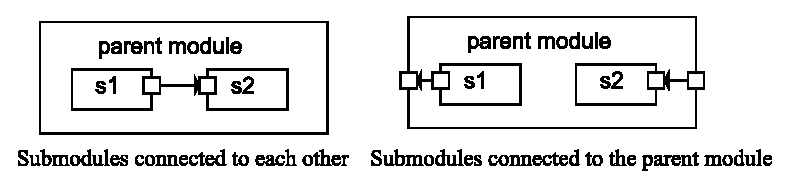
\includegraphics[width=5.061in, height=1.121in]{figures/usmanFig3}
\caption{Connections}
\label{fig:ch-overview:connections}
\end{center}
\end{figure}

Due to the hierarchical structure of the model, messages typically
travel through a series of connections, to start and arrive in simple
modules. Such series of connections that go from simple module to
simple module are called \textit{routes}.  Compound modules act as
'cardboard boxes' in the model, transparently relaying messages
between their inside and their outside world.


\subsection{Link characteristics}

Connections can be assigned three parameters which facilitate 
the modeling of communication networks, but can be useful for 
other models too:
\begin{itemize}
  \item{propagation delay (sec)\index{channel!propagation delay}}
  \item{bit error rate (errors/bit)\index{channel!bit error rate}}
  \item{data rate (bits/sec)\index{channel!data rate}}
\end{itemize}


Each of these parameters is optional. One can specify link parameters 
individually for each connection, or define link types (also 
called \textit{channel} \textit{types}) once and use them throughout the 
whole model.

The \textit{propagation delay} is the amount of time the arrival of 
the message is delayed by when it travels through the channel. 
Propagation delay is specified in seconds.

The \textit{bit error rate} has influence on the transmission of messages 
through the channel. The bit error rate is the probability that 
a bit is incorrectly transmitted. Thus, the probability that 
a message of \textit{n} bits length is transferred correctly is:\\


$P( \textit{sent message received properly} ) = (1 - \textit{ber})^{\mathit{n}}$\\
where \textit{ber} = bit error rate and \textit{n} = number of bits in message.\\


The message has an error flag which is set in case of transmission 
errors.

The \textit{data rate} is specified in bits/second, and it is used 
for transmission delay calculation. The sending time of the message 
normally corresponds to the transmission of the first bit, and 
the arrival time of the message corresponds to the reception 
of the last bit (Fig. \ref{fig:ch-overview:message-transm}).

\begin{figure}[htbp]
\begin{center}
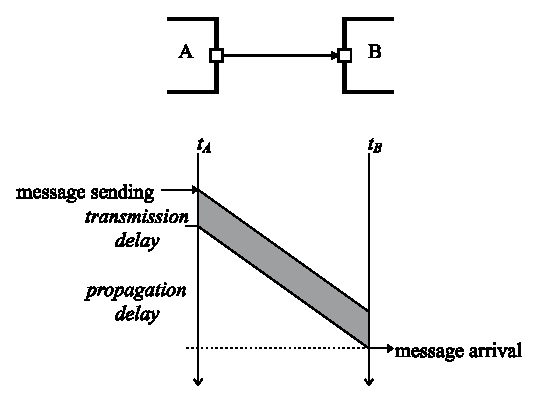
\includegraphics[width=4.301in, height=2.417in]{figures/usmanFig4}
\caption{Message transmission}
\label{fig:ch-overview:message-transm}
\end{center}
\end{figure}

The above model is not applicable for modeling some protocols like
Token Ring and FDDI where the stations repeat the bits of a frame that
arrives on the ring immediately, without waiting for the whole frame
to arrive; in other words, frames ''flow through'' the stations, being
delayed only a few bits. If you want to model such networks, the data
rate modeling feature of {\opp} cannot be used.

If a message travels along a route, through successive links and
compound modules, the model behaves as if each module waited until the
last bit of the message arrives and only start its transmission then
(Fig. \ref{fig:ch-overview:msg-multiple-ch}).

\begin{figure}[htbp]
\begin{center}
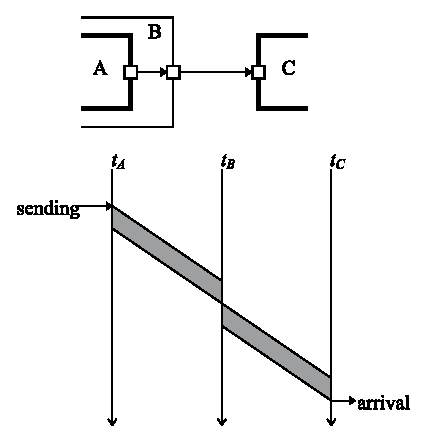
\includegraphics[width=3.330in, height=2.692in]{figures/usmanFig5}
\caption{Message sending over multiple channels}
\label{fig:ch-overview:msg-multiple-ch}
\end{center}
\end{figure}

Since the above effect is usually not the desired one, typically 
you will want to assign data rate to only one connection in the 
route.


\subsection{Parameters}
\index{module!parameters}
\index{parameters|see{module parameters}}

Modules can have parameters. Parameters are used for three purposes: 
\begin{enumerate}
  \item{to parameterize module topology}
  \item{to customize simple module behaviour}
  \item{for module communication, as shared variables}
\end{enumerate}

Parameters can take string, numeric or pointer values; numeric 
values include expressions using other parameters and calling 
C functions, random variables from different distributions, and 
values input interactively by the user.


Numeric-valued parameters can be used to construct topologies in a
flexible way. Within a compound module, parameters can define the
number of submodules, number of gates, and the way the internal
connections are made.


Compound modules can pass parameters or expressions of parameters 
to their submodules. Parameter passing can be done by value or 
by reference.

During simulation execution, if a module changes the value of 
a parameter taken by reference, the changed value propagates 
to other modules. This effect can be used to tune the model or 
as a second means of module communication. Pointer-valued parameters 
can be used to implement shared memory.


\subsection{Topology description method}
\index{topology!description}
The user defines the structure of the model in NED language descriptions 
(Network Description).The NED language will be discussed in detail 
in Chapter \ref{cha:the-ned-language}.


\section{Programming the algorithms}

The simple\index{module!simple} modules of a model contain the algorithms as C++ functions. 
The full flexibility and power of the programming language can 
be used, supported by the {\opp} simulation class library.


{\opp} supports a process-style\index{module!process-style} description method for describing 
activities. During simulation execution, simple\index{module!simple} module functions 
appear to run in parallel, because they are implemented as coroutines\index{module!coroutine} 
(also termed lightweight processes). Coroutines were chosen because 
they allow an intuitive description of the algorithm and they 
can also serve as a good basis for implementing other description 
methods like state-transition diagrams\index{state-transition diagram|see{finite state machine}} or Petri nets\index{petri nets}.

{\opp} has a consistent object-oriented design. One can freely 
use OOP concepts (inheritance, polymorphism etc) to extend the 
functionality of the simulator.

Elements of the simulation (messages, modules, queues etc.) are 
represented as objects. These classes are part of the simulation 
class library:
\begin{itemize}
\item{modules, gates, connections etc.}
\item{parameters}
\item{messages}
\item{container classes (e.g. queue, array)}
\item{data collection classes}
\item{statistic and distribution estimation classes (histograms, $P^{2}$ 
algorithm for calculating quantiles etc.)}
\item{transient detection and result accuracy detection classes}
\end{itemize}

The objects are designed so that they can efficiently work together, 
creating a powerful framework for simulation programming.


\subsection{Creating simple modules}
\index{module!simple!creation}

Each simple\index{module!simple} module type is implemented with a C++ class. Simple 
module classes are derived from a simple module base class, by 
redefining the virtual function that contains the algorithm. 
The user can add other member functions to the class to split 
up a complex algorithm; he can also add data members to the class. 

It is also possible to derive new simple\index{module!simple} module classes from 
existing ones. For example, if one wants to experiment with retransmission 
timeout schemes in a transport protocol, he can implement the 
protocol in one class, create a virtual function for the retransmission 
algorithm and then derive a family of classes that implement 
concrete schemes. This concept is further supported by the fact 
that in the network description, actual module types can be parameters.


\subsection{Object mechanisms}

The use of smart container classes allows the user to build
\textit{aggregate data structures}\index{aggregate data structures}.
For example, one can add any number of objects to a message object as
parameters. Since the added objects can contain further objects,
complex data structures can be built.

There is an efficient \textit{ownership}\index{ownership} mechanism
built in. The user can specify an owner for each object; then, the
owner object will have the responsibility of destroying that object.
Most of the time, the ownership mechanism works transparently;
ownership only needs to be explicitly managed when the user wants to
do something non-typical.


The \textit{forEach}\index{forEach mechanism} mechanism allows one to
enumerate the objects inside a container object in a uniform way and
do some operation on them. This feature which makes it possible to
handle many objects together. (The forEach feature is extensively used
by the user interfaces with debugging capability and the snapshot
mechanism; see later.)


\subsection{Derive new classes}

It most cases, the functionality offered by the {\opp} classes 
is enough for the user. But if it is needed, one can derive new 
classes from the existing ones or create entirely new classes. 
For flexibility, several member functions are declared virtual. 
When the user creates new classes, certain rules need to be kept 
so that the object can fully work together with other objects.


\subsection{Self-describing objects to ease debugging}
\index{debugging}

The class library is designed so that objects can give textual 
information about themselves. This makes it possible to peek 
into a running simulation program: through an appropriate user 
interface, one can examine (and modify) the internal data structures 
of a running simulation. This feature helps the user to get some 
insight what is happening inside the model and get hands-on experience.


A unique feature called \textit{snapshot}\index{snapshot} allows the
user to dump the contents of the simulation model or a part of it into
a text file. The file will contain textual reports about every object;
this can be of invaluable help at times of debugging. Ordinary
variables can also be made to appear in the snapshot file. Snapshot
creations can be scheduled from within the simulation program or done
from the user interface.



\section{Using {\opp}}


\subsection{Building and running simulations}
\index{simulation!building}
\index{simulation!running}

This section gives some idea how to work with {\opp} in practice: 
issues like model files, compiling and running simulations are 
discussed.

An {\opp} model consists of the following parts:
\begin{itemize}
  \item{NED language topology description(s)\index{ned!files} which
    describe the module structure with parameters, gates etc. They are
    files with .ned suffix. NED files can be written with any text
    editor or using the GNED graphical editor\index{ned!graphical interface}.}
  \item{ Simple modules sources. They are C++ files, with \texttt{.h}/\texttt{.cc} suffix.}
\end{itemize}

The simulation system provides the following components:
\begin{itemize}
  \item{Simulation kernel\index{simulation!kernel}. This contains the
    code that manages the simulation and the simulation class library.
    It is written in C++, compiled and put together to form a library
    (a file with .a or .lib extension)}
  \item{User interfaces\index{simulation!user interface}
    \index{user interface|see{simulation interface}}. {\opp} user interfaces
    are used with simulation execution, to facilitate debugging,
    demonstration, or batch execution of simulations. There are
    several user interfaces, written in C++, compiled and put together
    into libraries (\texttt{.a} or \texttt{.lib} files).}
\end{itemize}


Simulation programs are built from the above components. First, the
NED files\index{ned!files} are compiled into C++ source code, using
the NEDC\index{ned!compiler} compiler which is part of {\opp}. Then
all C++ sources are compiled and linked with the simulation kernel and
a user interface to form a simulation executable.


\textbf{Running the simulation and analyzing the results}

The simulation executable is a standalone program\footnote{as long as
  it is linked statically}; thus, it can be run on other machines
without {\opp} or the model files being present. When the program is
started, it reads in a configuration
file\index{simulation!configuration file} (usually called
\texttt{omnetpp.ini}\index{omnetpp.ini}); it contains settings that
control how the simulation is run, values for model parameters, etc.
The configuration file can also prescribe several simulation runs; in
the simplest case, they will be executed by the simulation program one
after another.

The output of the simulation is written into data files: output vector
files\index{output!vector file}, output scalar files
\index{output!scalar file}, and possibly the user's own output files.
{\opp} provides a GUI tool named Plove to view and plot the contents
of output vector files. But it is not expected that someone will
process the result files using {\opp} alone: output files are text
files in a format which (maybe after some preprocessing using
\fprog{sed}, \fprog{awk} or \fprog{perl}) can be read into math
packages like Matlab or its free equivalent Octave, or imported into
spreadsheets like Excel. All these external programs have rich
functionality for statistical analysis and visualization, and {\opp}
does not try to duplicate their efforts. This manual briefly describes
some data plotting programs and how to use them with {\opp}.


\textbf{User interfaces}
\index{simulation!user interface}

The primary purpose of user interfaces is to make the inside 
of the model visible to the user, to start/stop simulation execution, 
and possibly allow the user intervene by changing variables/objects 
inside the model. This is very important in the development/debugging 
phase of the simulation project. Just as important, a hands-on 
experience allows the user to get a 'feel' about the model's 
behaviour. A nice graphical user interface can also be used to 
demonstrate how the model works internally.


The same simulation model can be executed with different user 
interfaces, without any change in the model files themselves. 
The user would test and debug the simulation with a powerful 
graphical user interface, and finally run it with a simple and 
fast user interface that supports batch execution.


\textbf{Component libraries}
\index{module!libraries}

Module types can be stored in files separately from the place 
of their actual usage. This means that the user can group existing 
module types and create component libraries.


\textbf{Universal standalone simulation programs}


A simulation executable can store several independent models 
that use the same set of simple modules. The user can specify 
in the configuration file which model he/she wants to run. This 
allows one to build one large executable that contains several 
simulation models, and distribute it as a standalone simulation 
tool. The flexibility of the topology description language also 
supports this approach.


\subsection{What is what in the directories}

To help you navigate among files in the {\opp} distribution, 
here's a list what you can find in the different directories.

The \texttt{omnetpp} directory contains the following subdirectories.


%%\setlength\LTleft\parindent
\begin{longtable}{l@{\extracolsep{1cm}}p{8cm}}
  \multicolumn{2}{p{\textwidth}}{The simulation system itself:}\\
  \textbf{omnetpp/} & {\opp} root directory\\
  \tab\textbf{bin/} & {\opp} executables (GNED, nedc, etc.) \\
  \tab\textbf{include/} & header files for simulation models\\
  \tab\textbf{lib/} & library files\\
  \tab\textbf{bitmaps/} & icons that can be used in network graphics\\
  \tab\textbf{doc/} & manual (PDF), readme, license, etc. \\
  \tab\tab\textbf{html/} & manual in HTML\\
  \tab\tab \textbf{api/} & API reference in HTML\\
  \tab\textbf{src/} & {\opp} sources \\
  \tab\tab\textbf{nedc/} & NED compiler\index{ned!compiler} \\
  \tab\tab\textbf{sim/} & simulation kernel \\
  \tab\tab\tab\textbf{std/} & files for non-distributed execution \\
  \tab\tab\tab\textbf{pvm/} & files for distributed execution over PVM \\
  \tab\tab\tab\textbf{mpi/} & files for distributed execution using MPI \\
  \tab\tab\textbf{envir/} & common code for user interfaces \\
  \tab\tab\textbf{cmdenv/} & command-line user interface \\
  \tab\tab\textbf{tkenv/} & Tcl/Tk-based user interface \\
  \tab\tab\textbf{gned/} & graphical NED editor\index{ned!graphical interface} \\
  \tab\tab\textbf{plove/} & output vector analyzer and plotting tool \\
  \tab\tab\textbf{utils/} & makefile-autocreator etc\\
   & \\
  \multicolumn{2}{p{\textwidth}}{There is a tutorial, contributed by Nick van Foreest}\\
  \tab\textbf{tutorial/} & the tutorial document \\
  \tab\tab\textbf{queues/} & sample simulation that supports the tutorial\\
  \tab\tab\textbf{doc\_src/} & the Latex sources for the tutorial doc\\
   & \\
  \multicolumn{2}{p{\textwidth}}{Sample simulations are within the \texttt{samples}
  directory. Each of the sample directories contain a network
  description (.ned file) and corresponding simple module code (\texttt{.h},
  \texttt{.cc} files). Makefiles are included.}\\
  \tab\textbf{samples/} & directories for sample simulations\\
  \tab\tab\textbf{nim/} & a simple two-player game \\
  \tab\tab\textbf{hcube/} & hypercube network with deflection routing \\
  \tab\tab\textbf{token/} & Token-Ring network \\
  \tab\tab\textbf{fddi/} & an accurate FDDI MAC simulation \\
  \tab\tab\textbf{hist/} & demo of the histogram classes \\
  \tab\tab\textbf{dyna/} & dynamic module creation (client-server network) \\
  \tab\tab\textbf{pvmex/} & demonstrates distributed execution \\
  \tab\tab\textbf{fifo1/} & single-server queue \\
  \tab\tab\textbf{fifo2/} & another implementation of a single-server queue \\
  \tab\tab\textbf{demo/} & several sim. models in a single executable \\
   & \\
  \multicolumn{2}{p{\textwidth}}{The \texttt{contrib} directory contains material from the {\opp} community}\\
  \tab\textbf{contrib/} & directory for contributed material \\
  \tab\textbf{octave/} & Octave scripts for result processing\\
  \tab\textbf{emacs/} & NED syntax highlight for Emacs
\end{longtable}

You may also find additional directories like \texttt{msvc/}, which contains 
integration components for Microsoft Visual C++, etc.\\


%%% Local Variables: 
%%% mode: latex
%%% TeX-master: "usman"
%%% End: 

\cleardoublepage

\chapter{The NED Language}
\label{cha:ned-lang}


\section{NED Overview}
\label{sec:ned-lang:ned-overview}

The user describes the structure of a simulation model in the NED language. NED
stands for Network Description. NED lets the user declare simple modules, and
connect and assemble them into compound modules. The user can label some compound
modules as \textit{networks}; that is, self-contained simulation models. Channels are
another component type, whose instances can also be used in compound modules.

The NED language has several features which let it scale well to large projects:

\begin{description}

\item[Hierarchical.] The traditional way to deal with complexity is by
introducing hierarchies. In {\opp}, any module which would be too complex as
a single entity can be broken down into smaller modules, and used as a
compound module.

\item[Component-Based.] Simple modules and compound modules are inherently
reusable, which not only reduces code copying, but more importantly, allows
component libraries (like the INET Framework, MiXiM, Castalia, etc.) to
exist.

\item[Interfaces.] Module and channel interfaces can be used as a
placeholder where normally a module or channel type would be used, and the
concrete module or channel type is determined at network setup time by a
parameter. Concrete module types have to ``implement'' the interface they
can substitute. For example, given a compound module type named
\ttt{MobileHost} contains a \ttt{mobility} submodule of the type
\ttt{IMobility} (where \ttt{IMobility} is a module interface), the actual
type of \ttt{mobility} may be chosen from the module types that implemented
\ttt{IMobility} (\ttt{RandomWalkMobility}, \ttt{TurtleMobility}, etc.)

\item[Inheritance.] Modules and channels can be subclassed. Derived modules
and channels may add new parameters, gates, and (in the case of compound
modules) new submodules and connections. They may set existing parameters
to a specific value, and also set the gate size of a gate vector. This
makes it possible, for example, to take a \ttt{GenericTCPClientApp} module
and derive an \ttt{FTPClientApp} from it by setting certain parameters to a fixed
value; or to derive a \ttt{WebClientHost} compound module from a
\ttt{BaseHost} compound module by adding a \ttt{WebClientApp} submodule and
connecting it to the inherited \ttt{TCP} submodule.

\item[Packages.] The NED language features a Java-like package structure,
to reduce the risk of name clashes between different models. \ttt{NEDPATH}
(similar to Java's \ttt{CLASSPATH}) has also been introduced to make it easier
to specify dependencies among simulation models.

\item[Inner types.] Channel types and module types used locally by a
compound module can be defined within the compound module, in order to
reduce namespace pollution.

\item[Metadata annotations.] It is possible to annotate module or channel
types, parameters, gates and submodules by adding properties. Metadata are
not used by the simulation kernel directly, but they can carry extra
information for various tools, the runtime environment, or even for other
modules in the model. For example, a module's graphical representation
(icon, etc)  or the prompt string and measurement unit (milliwatt, etc) of a
parameter are already specified as metadata annotations.

\end{description}

\begin{note}
    The NED language has changed significantly in the 4.0 version.
    Inheritance, interfaces, packages, inner types, metadata annotations, inout
    gates were all added in the 4.0 release, together with many other features.
    Since the basic syntax has changed as well, old NED files need to be
    converted to the new syntax. There are automated tools for this purpose, so
    manual editing is only needed to take advantage of new NED features.
\end{note}

The NED language has an equivalent tree representation which can be
serialized to XML; that is, NED files can be converted to XML and back
without loss of data, including comments. This lowers the barrier for
programmatic manipulation of NED files; for example extracting information,
refactoring and transforming NED, generating NED from information stored in
other systems like SQL databases, and so on.

\begin{note}
    This chapter is going to explain the NED language gradually, via examples.
    If you are looking for a more formal and concise treatment, see
    Appendix \ref{cha:ned-language-grammar}.
\end{note}


\section{NED Quickstart}
\label{sec:ned-lang:warmup}

In this section we introduce the NED language via a complete and
reasonably real-life example: a communication network.

Our hypothetical network consists of nodes. On each node there is an
application running which generates packets at random intervals.
The nodes are routers themselves as well. We assume that the application
uses datagram-based communication, so that we can leave out the
transport layer from the model.


\subsection{The Network}
\label{sec:ned-lang:warmup:network}

First we'll define the network, then in the next sections we'll continue
to define the network nodes.

Let the network topology be as in Figure \ref{fig:ned-routing-topology}.

\begin{figure}[htbp]
  \begin{center}
    \includepng[scale=0.6]{figures/ned-routing-network}
    \caption{The network}
    \label{fig:ned-routing-topology}
  \end{center}
\end{figure}

The corresponding NED description would look like this:

\begin{ned}
//
// A network
//
network Network
{
    submodules:
        node1: Node;
        node2: Node;
        node3: Node;
        ...
    connections:
        node1.port++ <--> {datarate=100Mbps;} <--> node2.port++;
        node2.port++ <--> {datarate=100Mbps;} <--> node4.port++;
        node4.port++ <--> {datarate=100Mbps;} <--> node6.port++;
        ...
}
\end{ned}

The above code defines a network type named \ttt{Network}. Note that the NED
language uses the familiar curly brace syntax, and ``\ttt{//}'' to denote
comments.

\begin{note}
    Comments in NED not only make the source code more readable, but in the
    {\opp} IDE they also are displayed at various places (tooltips, content
    assist, etc), and become part of the documentation extracted from the NED
    files. The NED documentation system, not unlike \textit{JavaDoc} or
    \textit{Doxygen}, will be described in Chapter \ref{cha:neddoc}.
\end{note}

The network contains several nodes, named \ttt{node1}, \ttt{node2}, etc.
from the NED module type \ttt{Node}. We'll define \ttt{Node} in the next
sections.

The second half of the declaration defines how the nodes are to be
connected. The double arrow means bidirectional connection. The connection
points of modules are called gates, and the \ttt{port++} notation adds a
new gate to the \ttt{port[]} gate vector. Gates and connections will be
covered in more detail in sections \ref{sec:ned-lang:gates} and
\ref{sec:ned-lang:connections}. Nodes are connected with a channel that
has a data rate of 100Mbps.

\begin{note}
    In many other systems, the equivalent of {\opp} gates are called
    \textit{ports}. We have retained the term \textit{gate} to reduce
    collisions with other uses of the otherwise overloaded word
    \textit{port}: router port, TCP port, I/O port, etc.
\end{note}

The above code would be placed into a file named \ttt{Net6.ned}. It is
a convention to put every NED definition into its own file and to name the
file accordingly, but it is not mandatory to do so.

One can define any number of networks in the NED files, and for every
simulation the user has to specify which network to set up.
The usual way of specifying the network is to put the \fconfig{network}
option into the configuration (by default the \ffilename{omnetpp.ini} file):

\begin{inifile}
[General]
network = Network
\end{inifile}


\subsection{Introducing a Channel}
\label{sec:ned-lang:warmup:introducing-a-channel}

It is cumbersome to have to repeat the data rate for every connection.
Luckily, NED provides a convenient solution: one can create a new channel
type that encapsulates the data rate setting, and this channel type can
be defined inside the network so that it does not litter the global
namespace.

The improved network will look like this:

\begin{ned}
//
// A Network
//
network Network
{
    types:
        channel C extends ned.DatarateChannel {
            datarate = 100Mbps;
        }
    submodules:
        node1: Node;
        node2: Node;
        node3: Node;
        ...
    connections:
        node1.port++ <--> C <--> node2.port++;
        node2.port++ <--> C <--> node4.port++;
        node4.port++ <--> C <--> node6.port++;
        ...
}
\end{ned}

Later sections will cover the concepts used (inner types, channels, the
\ttt{DatarateChannel} built-in type, inheritance) in detail.


\subsection{The App, Routing, and Queue Simple Modules}
\label{sec:ned-lang:warmup:the-simple-modules}

Simple modules are the basic building blocks for other (compound) modules,
denoted by the \fkeyword{simple} keyword.
All active behavior in the model is encapsulated in \fkeyword{simple} modules.
Behavior is defined with a C++ class; NED files only declare the externally
visible interface of the module (gates, parameters).

In our example, we could define \ttt{Node} as a simple module. However,
its functionality is quite complex (traffic generation, routing, etc),
so it is better to implement it with several smaller simple module types
which we are going to assemble into a compound module. We'll have
one simple module for traffic generation (\ttt{App}), one for routing
(\ttt{Routing}), and one for queueing up packets to be sent out (\ttt{Queue}).
For brevity, we omit the bodies of the latter two in the code below.

\begin{ned}
simple App
{
    parameters:
        int destAddress;
        ...
        @display("i=block/browser");
    gates:
        input in;
        output out;
}

simple Routing
{
    ...
}

simple Queue
{
    ...
}
\end{ned}

By convention, the above simple module declarations go into the
\ttt{App.ned}, \ttt{Routing.ned} and \ttt{Queue.ned} files.

\begin{note}
    Note that module type names (\ttt{App}, \ttt{Routing}, \ttt{Queue})
    begin with a capital letter, and parameter and gate names begin with
    lowercase -- this is the recommended naming convention. Capitalization
    matters because the language is case sensitive.
\end{note}

Let us look at the first simple module type declaration. \ttt{App} has a
parameter called \ttt{destAddress} (others have been omitted for now),
and two gates named \ttt{out} and \ttt{in} for sending and receiving
application packets.

The argument of \fprop{@display()} is called a \textit{display string},
and it defines the rendering of the module in graphical environments;
\ttt{"i=..."} defines the default icon.

Generally, \ttt{@}-words like \ttt{@display} are called \textit{properties}
in NED, and they are used to annotate various objects
with metadata. Properties can be attached to files, modules, parameters, gates,
connections, and other objects, and parameter values have a very flexible
syntax.


\subsection{The Node Compound Module}
\label{sec:warmup:ned-lang:node-compound-module}

Now we can assemble \ttt{App}, \ttt{Routing} and \ttt{Queue} into the
compound module \ttt{Node}. A compound module can be thought of as
a ``cardboard box'' that groups other modules into a larger unit,
which can further be used as a building block for other modules;
networks are also a kind of compound module.

\begin{figure}[htbp]
  \begin{center}
    \includepng[scale=0.6]{figures/ned-routing-node}
    \caption{The Node compound module}
    \label{fig:ned-routing-node}
  \end{center}
\end{figure}

\begin{ned}
module Node
{
    parameters:
        int address;
        @display("i=misc/node_vs,gold");
    gates:
        inout port[];
    submodules:
        app: App;
        routing: Routing;
        queue[sizeof(port)]: Queue;
    connections:
        routing.localOut --> app.in;
        routing.localIn <-- app.out;
        for i=0..sizeof(port)-1 {
            routing.out[i] --> queue[i].in;
            routing.in[i] <-- queue[i].out;
            queue[i].line <--> port[i];
        }
}
\end{ned}

Compound modules, like simple modules, may have parameters and gates.
Our \ttt{Node} module contains an \ttt{address} parameter, plus a
\textit{gate vector} of unspecified size, named \ttt{port}.
The actual gate vector size will be determined implicitly by the number
of neighbours when we create a network from nodes of this type.
The type of \ttt{port[]} is \ttt{inout}, which allows bidirectional
connections.

The modules that make up the compound module are listed under
\fkeyword{submodules}. Our \ttt{Node} compound module type has an \ttt{app} and
a \ttt{routing} \textit{submodule}, plus a \ttt{queue[]} \textit{submodule
vector} that contains one \ttt{Queue} module for each port, as specified by
\ttt{[sizeof(port)]}. (It is legal to refer to \ttt{[sizeof(port)]} because
the network is built in top-down order, and the node is already created and
connected at network level when its submodule structure is built out.)

In the \fkeyword{connections} section, the submodules are connected to each
other and to the parent module. Single arrows are used to connect input and
output gates, and double arrows connect inout gates, and a \fkeyword{for} loop
is utilized to connect the \ttt{routing} module to each \ttt{queue} module, and
to connect the outgoing/incoming link (\ttt{line} gate) of each queue to the
corresponding port of the enclosing module.


\subsection{Putting It Together}
\label{sec:ned-lang:warmup:putting-it-together}

We have created the NED definitions for this example, but how are they used by {\opp}? When
the simulation program is started, it loads the NED files. The program
should already contain the C++ classes that implement the needed simple
modules, \ttt{App}, \ttt{Routing} and \ttt{Queue}; their C++ code is either
part of the executable or is loaded from a shared library. The simulation
program also loads the configuration (\ffilename{omnetpp.ini}), and determines
from it that the simulation model to be run is the \ttt{Network} network.
Then the network is instantiated for simulation.

The simulation model is built in a top-down preorder fashion. This means
that starting from an empty system module, all submodules are created,
their parameters and gate vector sizes are assigned, and they are fully connected
before the submodule internals are built.

\bigskip
\begin{center}
* * *
\end{center}
\bigskip

In the following sections we'll go through the elements of the NED
language and look at them in more detail.



\section{Simple Modules}
\label{sec:ned-lang:simple-modules}

Simple modules are the active components in the model.
Simple modules are defined with the \fkeyword{simple} keyword.

An example simple module:

\begin{ned}
simple Queue
{
    parameters:
        int capacity;
        @display("i=block/queue");
    gates:
        input in;
        output out;
}
\end{ned}

Both the \fkeyword{parameters} and \fkeyword{gates} sections are optional, that is,
they can be left out if there is no parameter or gate. In addition, the
\fkeyword{parameters} keyword itself is optional too; it can be left out
even if there are parameters or properties.

Note that the NED definition doesn't contain any code to define the
operation of the module: that part is expressed in C++. By default, {\opp}
looks for C++ classes of the same name as the NED type (so here, \ttt{Queue}).

One can explicitly specify the C++ class with the \fprop{@class} property.
Classes with namespace qualifiers are also accepted, as shown in the following
example that uses the \ttt{mylib::Queue} class:

\begin{ned}
simple Queue
{
    parameters:
        int capacity;
        @class(mylib::Queue);
        @display("i=block/queue");
    gates:
        input in;
        output out;
}
\end{ned}

If you have several modules that are all in a common namespace, then a
better alternative to \fprop{@class} is the \fprop{@namespace} property. The
C++ namespace given with \fprop{@namespace} will be prepended to the normal
class name. In the following example, the C++ classes will be
\ttt{mylib::App}, \ttt{mylib::Router} and \ttt{mylib::Queue}:

\begin{ned}
@namespace(mylib);

simple App {
   ...
}

simple Router {
   ...
}

simple Queue {
   ...
}
\end{ned}

As you've seen, \fprop{@namespace} can be specified at the file level. Moreover,
when placed in a file called \ttt{package.ned}, the namespace will apply to
all files in the same directory and all directories below.

The implementation C++ classes need to be subclassed from the
\cclass{cSimpleModule} library class; chapter \ref{cha:simple-modules} of
this manual describes in detail how to write them.

Simple modules can be extended (or specialized) via subclassing. The
motivation for subclassing can be to set some open parameters or gate sizes
to a fixed value (see \ref{sec:ned-lang:parameters} and
\ref{sec:ned-lang:gates}), or to replace the C++ class with a different
one. Now, by default, the derived NED module type will \textit{inherit} the
C++ class from its base, so it is important to remember that you need to
write out \fprop{@class} if you want it to use the new class.

The following example shows how to specialize a module by setting a parameter
to a fixed value (and leaving the C++ class unchanged):

\begin{ned}
simple Queue
{
   int capacity;
   ...
}

simple BoundedQueue extends Queue
{
   capacity = 10;
}
\end{ned}

In the next example, the author wrote a \ttt{PriorityQueue} C++ class, and
wants to have a corresponding NED type, derived from \ttt{Queue}. However,
it does not work as expected:

\begin{ned}
simple PriorityQueue extends Queue // wrong! still uses the Queue C++ class
{
}
\end{ned}

The correct solution is to add a \fprop{@class} property to override the
inherited C++ class:

\begin{ned}
simple PriorityQueue extends Queue
{
   @class(PriorityQueue);
}
\end{ned}

Inheritance in general will be discussed in section \ref{sec:ned-lang:inheritance}.



\section{Compound Modules}
\label{sec:ned-lang:compound-modules}

A compound module groups other modules into a larger unit. A compound
module may have gates and parameters like a simple module, but no active
behavior is associated with it.\footnote{Although the C++ class
for a compound module can be overridden with the \fprop{@class} property,
this is a feature that should probably never be used. Encapsulate the code
into a simple module, and add it as a submodule.}

\begin{note}
    When there is a temptation to add code to a compound module,
    then encapsulate the code into a simple module, and add it as
    a submodule.
\end{note}

A compound module declaration may contain several sections,
all of them optional:

\begin{ned}
module Host
{
   types:
       ...
   parameters:
       ...
   gates:
       ...
   submodules:
       ...
   connections:
       ...
}
\end{ned}

Modules contained in a compound module are called submodules, and they are
listed in the \ttt{submodules} section. One can create arrays of submodules
(i.e. submodule vectors), and the submodule type may come from a parameter.

Connections are listed under the \ttt{connections} section of the
declaration. One can create connections using simple programming constructs
(loop, conditional). Connection behaviour can be defined by associating a
channel with the connection; the channel type may also come from a
parameter.

Module and channel types only used locally can be defined in the
\ttt{types} section as inner types, so that they do not pollute the
namespace.

Compound modules may be extended via subclassing. Inheritance may add new
submodules and new connections as well, not only parameters and gates.
Also, one may refer to inherited submodules, to inherited types etc. What
is not possible is to "de-inherit" or modify submodules or connections.

In the following example, we show how to assemble common protocols
into a "stub" for wireless hosts, and add user agents via
subclassing.\footnote{Module types, gate names, etc. used in the example
are fictional, not based on an actual {\opp}-based model framework}

\begin{ned}
module WirelessHostBase
{
   gates:
       input radioIn;
   submodules:
       tcp: TCP;
       ip: IP;
       wlan: Ieee80211;
   connections:
       tcp.ipOut --> ip.tcpIn;
       tcp.ipIn <-- ip.tcpOut;
       ip.nicOut++ --> wlan.ipIn;
       ip.nicIn++ <-- wlan.ipOut;
       wlan.radioIn <-- radioIn;
}

module WirelessHost extends WirelessHostBase
{
   submodules:
       webAgent: WebAgent;
   connections:
       webAgent.tcpOut --> tcp.appIn++;
       webAgent.tcpIn <-- tcp.appOut++;
}
\end{ned}

The \ttt{WirelessHost} compound module can further be extended,
for example with an Ethernet port:

\begin{ned}
module DesktopHost extends WirelessHost
{
   gates:
       inout ethg;
   submodules:
       eth: EthernetNic;
   connections:
       ip.nicOut++ --> eth.ipIn;
       ip.nicIn++ <-- eth.ipOut;
       eth.phy <--> ethg;
}
\end{ned}



\section{Channels}
\label{sec:ned-lang:channels}

Channels encapsulate parameters and behaviour associated with connections.
Channels are like simple modules, in the sense that there are C++ classes
behind them. The rules for finding the C++ class for a NED channel type is
the same as with simple modules: the default class name is the NED type
name unless there is a \fprop{@class} property (\fprop{@namespace} is also
recognized), and the C++ class is inherited when the channel is subclassed.

Thus, the following channel type would expect a \ttt{CustomChannel} C++ class
to be present:

\begin{ned}
channel CustomChannel  // requires a CustomChannel C++ class
{
}
\end{ned}

The practical difference compared to modules is that you rarely need to write you own
channel C++ class because there are predefined channel types that you can
subclass from, inheriting their C++ code. The predefined types are:
\ttt{ned.IdealChannel}, \ttt{ned.Delay\-Channel} and \ttt{ned.Datarate\-Channel}.
(``\ttt{ned}'' is the package name; you can get rid of it if you import the types
with the \ttt{import ned.*} or similar directive. Packages and imports
are described in section \ref{sec:ned-lang:packages}.)

\ttt{IdealChannel} has no parameters, and lets through all messages without
delay or any side effect. A connection without a channel object
and a connection with an \ttt{IdealChannel} behave in the same way.
Still, \ttt{IdealChannel} has its uses, for example when a channel object
is required so that it can carry a new property or parameter that is
going to be read by other parts of the simulation model.

\ttt{DelayChannel} has two parameters:

\begin{itemize}
    \item \ttt{delay} is a \ttt{double} parameter which represents the
          propagation delay of the message. Values need to be specified
          together with a time unit (\ttt{s}, \ttt{ms}, \ttt{us}, etc.)
    \item \ttt{disabled} is a boolean parameter that defaults to \ttt{false};
          when set to \ttt{true}, the channel object will drop all messages.
\end{itemize}

\ttt{DatarateChannel} has a few additional parameters compared to \ttt{DelayChannel}:

\begin{itemize}
    \item \ttt{datarate} is a \ttt{double} parameter that represents the
          data rate of the channel. Values need to be specified
          in bits per second or its multiples as unit (\ttt{bps},
          \ttt{kbps}, \ttt{Mbps}, \ttt{Gbps}, etc.) Zero is treated
          specially and results in zero transmission duration, i.e.
          it stands for infinite bandwidth. Zero is also the default.
          Data rate is used for calculating the transmission duration of
          packets.
    \item \ttt{ber} and \ttt{per} stand for Bit Error Rate and Packet Error Rate,
          and allow basic error modelling. They expect a \ttt{double}
          in the $[0,1]$ range. When the channel decides (based on random
          numbers) that an error occurred during transmission of a packet,
          it sets an error flag in the packet object. The receiver
          module is expected to check the flag, and discard the packet
          as corrupted if it is set. The default \ttt{ber} and \ttt{per}
          are zero.
\end{itemize}

\begin{note}
    There is no channel parameter that specifies whether the channel
    delivers the message object to the destination module at the end or
    at the start of the reception; that is decided by the C++ code
    of the target simple module. See the \ffunc{setDeliverOn\-Reception\-Start()}
    method of \cclass{cGate}.
\end{note}

The following example shows how to create a new channel type by
specializing \ttt{DatarateChannel}:

\begin{ned}
channel Ethernet100 extends ned.DatarateChannel
{
    datarate = 100Mbps;
    delay = 100us;
    ber = 1e-10;
}
\end{ned}

\begin{note}
    The three built-in channel types are also used for connections where
    the channel type is not explicitly specified.
\end{note}

You may add parameters and properties to channels via subclassing, and
may modify existing ones. In the following example, we introduce distance-based
calculation of the propagation delay:

\begin{ned}
channel DatarateChannel2 extends ned.DatarateChannel
{
    double distance @unit(m);
    delay = this.distance / 200000km * 1s;
}
\end{ned}

Parameters are primarily useful as input to the underlying C++ class, but
even if you reuse the underlying C++ class of built-in channel types, they
may be read and used by other parts of the model. For example, adding a
\ttt{cost} parameter (or \fprop{@cost} property) may be observed by the
routing algorithm and used for routing decisions. The following example
shows a \ttt{cost} parameter, and annotation using a property
(\fprop{@backbone}).

\begin{ned}
channel Backbone extends ned.DatarateChannel
{
    @backbone;
    double cost = default(1);
}
\end{ned}



\section{Parameters}
\label{sec:ned-lang:parameters}

Parameters are variables that belong to a module. Parameters can be
used in building the topology (number of nodes, etc), and to supply
input to C++ code that implements simple modules and channels.

Parameters can be of type \fkeyword{double}, \fkeyword{int},
\fkeyword{bool}, \fkeyword{string} and \fkeyword{xml}; they can also
be declared \fkeyword{volatile}. For the numeric types, a unit of
measurement can also be specified (\fprop{@unit} property), to increase
type safety.

Parameters can get their value from NED files or from the configuration
(\ffilename{omnetpp.ini}). A default value can also be given (\ttt{default(}...\ttt{)}),
which is used if the parameter is not assigned otherwise.

The following example shows a simple module that has five parameters, three
of which have default values:

\begin{ned}
simple App
{
    parameters:
        string protocol;       // protocol to use: "UDP" / "IP" / "ICMP" / ...
        int destAddress;       // destination address
        volatile double sendInterval @unit(s) = default(exponential(1s));
                               // time between generating packets
        volatile int packetLength @unit(byte) = default(100B);
                               // length of one packet
        volatile int timeToLive = default(32);
                               // maximum number of network hops to survive
    gates:
        input in;
        output out;
}
\end{ned}


\subsection{Assigning a Value}
\label{sec:ned-lang:parameter-assignments}

Parameters may get their values in several ways: from NED code, from the
configuration (\ffilename{omnetpp.ini}), or even, interactively from the
user. NED lets you assign parameters at several places: in subclasses via
inheritance; in submodule and connection definitions where the NED type is
instantiated; and in networks and compound modules that directly or
indirectly contain the corresponding submodule or connection.

For instance, one could specialize the above \ttt{App} module type via
inheritance with the following definition:

\begin{ned}
simple PingApp extends App
{
    parameters:
        protocol = "ICMP/ECHO"
        sendInterval = default(1s);
        packetLength = default(64byte);
}
\end{ned}

This definition sets the \ttt{protocol} parameter to a fixed value
(\ttt{"ICMP/ECHO"}), and changes the default values of the
\ttt{sendInterval} and \ttt{packetLength} parameters. \ttt{protocol} is now
locked down in \ttt{PingApp}, its value cannot be modified via further subclassing
or other ways. \ttt{sendInterval} and \ttt{packetLength} are still unassigned
here, only their default values have been overwritten.

Now, let us see the definition of a \ttt{Host} compound module that uses
\ttt{PingApp} as submodule:

\begin{ned}
module Host
{
    submodules:
        ping : PingApp {
            packetLength = 128B; // always ping with 128-byte packets
        }
        ...
}
\end{ned}

This definition sets the \ttt{packetLength} parameter to a fixed value. It
is now hardcoded that \ttt{Host}s send 128-byte ping packets; this
setting cannot be changed from NED or the configuration.

It is not only possible to set a parameter from the compound module that
contains the submodule, but also from modules higher up in the module tree.
If you had a network that employed several \ttt{Host} modules, it could be
defined like this:

\begin{ned}
network Network
{
    submodules:
        host[100]: Host {
            ping.timeToLive = default(3);
            ping.destAddress = default(0);
        }
        ...
}
\end{ned}

Parameter assignment can also be placed into the \ttt{parameters} block of
the parent compound module, which provides additional flexibility. The
following definition sets up the hosts so that half of them pings host \#50,
and the other half pings host \#0:

\begin{ned}
network Network
{
    parameters:
        host[*].ping.timeToLive = default(3);
        host[0..49].ping.destAddress = default(50);
        host[50..].ping.destAddress = default(0);

    submodules:
        host[100]: Host;
        ...
}
\end{ned}

Note the use of asterisk to match any index, and \ttt{..} to match index ranges.

If you had a number of individual hosts instead of a submodule vector,
the network definition could look like this:

\begin{ned}
network Network
{
    parameters:
        host*.ping.timeToLive = default(3);
        host{0..49}.ping.destAddress = default(50);
        host{50..}.ping.destAddress = default(0);

    submodules:
        host0: Host;
        host1: Host;
        host2: Host;
        ...
        host99: Host;
}
\end{ned}

An asterisk matches any substring not containing a dot, and a \ttt{..}
within a pair of curly braces matches a natural number embedded in a
string.

In most assigments we have seen above, the left hand side of the equal sign
contained a dot and often a wildcard as well (asterisk or numeric range);
we call these assignments \textit{pattern assignments} or \textit{deep
assignments}.

There is one more wildcard that can be used in pattern assignments, and
this is the double asterisk; it matches any sequence of characters
including dots, so it can match multiple path elements. An example:

\begin{ned}
network Network
{
    parameters:
        **.timeToLive = default(3);
        **.destAddress = default(0);
    submodules:
        host0: Host;
        host1: Host;
        ...
}
\end{ned}

Note that some assignments in the above examples changed default values,
while others set parameters to fixed values. Parameters that received no
fixed value in the NED files can be assigned from the configuration
(\ffilename{omnetpp.ini}).

\begin{important}
    A non-default value assigned from NED cannot be overwritten later in
    NED or from ini files; it becomes ``hardcoded'' as far as ini files
    and NED usage are concerned. In contrast, default values are possible
    to overwrite.
\end{important}

A parameter can be assigned in the configuration using a similar syntax as
NED pattern assignments (actually, it would be more historically accurate
to say it the other way round, that NED pattern assignments use a similar
syntax to ini files):

%% FIXME show patterns for channel parameters too!

\begin{inifile}
Network.host[*].ping.sendInterval = 500ms  # for the host[100] example
Network.host*.ping.sendInterval = 500ms    # for the host0,host1,... example
**.sendInterval = 500ms
\end{inifile}

One often uses the double asterisk to save typing. You can write

\begin{inifile}
**.ping.sendInterval = 500ms
\end{inifile}

Or if you are sure that you don't accidentally assign some other
\ttt{sendInterval} parameter, you can just write

\begin{inifile}
**.sendInterval = 500ms
\end{inifile}

Parameter assignments in the configuration are described in section
\ref{sec:config-sim:parameter-settings}.

One can also write expressions, including stochastic expressions, in
NED files and in ini files as well. For example, here's how you can
add jitter to the sending of ping packets:

\begin{inifile}
**.sendInterval = 1s + normal(0s, 0.001s)  # or just: normal(1s, 0.001s)
\end{inifile}

If there is no assignment for a parameter in NED or in the ini file, the
default value (given with \ttt{=default(...)} in NED) will be applied
implicitly. If there is no default value, the user will be asked, provided
the simulation program is allowed to do that; otherwise there will be an
error. (Interactive mode is typically disabled for batch executions where
it would do more harm than good.)

It is also possible to explicitly apply the default (this can sometimes
be useful):

\begin{inifile}
**.sendInterval = default
\end{inifile}

Finally, one can explicitly ask the simulator to prompt the user interactively
for the value (again, provided that interactivity is enabled; otherwise
this will result in an error):

\begin{inifile}
**.sendInterval = ask
\end{inifile}

\begin{note}
    How do you decide whether to assign a parameter from NED or from an ini
    file? The advantage of ini files is that they allow a cleaner separation of the \textit{model}
    and \textit{experiments}. NED files (together with C++ code) are considered
    to be part of the model, and to be more or less constant. Ini files, on
    the other hand, are for experimenting with the model by running it
    several times with different parameters. Thus, parameters that are expected
    to change (or make sense to be changed) during experimentation should be
    put into ini files.
\end{note}


\subsection{Expressions}
\label{sec:ned-lang:expressions}

Parameter values may be given with expressions. NED language expressions
have a C-like syntax, with some variations on operator names: binary and
logical XOR are \ttt{\#} and \ttt{\#\#}, while \ttt{\^} has been reassigned
to \textit{power-of} instead. The \ttt{+} operator does string
concatenation as well as numeric addition. Expressions can use various
numeric, string, stochastic and other functions (\ttt{fabs()}, \ttt{toUpper()},
\ttt{uniform()}, \ttt{erlang\_k()}, etc.).

\begin{note}
    The list of NED functions can be found in Appendix \ref{cha:ned-functions}.
    The user can also extend NED with new functions.
\end{note}

%% XXX also sources of random numbers

Expressions may refer to module parameters, gate vector and module vector sizes
(using the \fkeyword{sizeof} operator) and the index of the current module
in a submodule vector (\fkeyword{index}).

%% XXX note: fullPath() etc functions!

Expressions may refer to parameters of the compound module being defined,
of the current module (with the \ttt{this.} prefix), and to parameters
of already defined submodules, with the syntax \ttt{submodule.parametername}
(or \ttt{submodule[index].parametername}).

%% XXX example: address = address;  delay=this.distance/this.speed;

%% XXX there are no parameter arrays, but... demonstrate the choose() function


\subsection{volatile}
\label{sec:ned-lang:volatile}

The \fkeyword{volatile} modifier causes the parameter's value expression to
be evaluated every time the parameter is read. This has significance if the
expression is not constant, for example it involves numbers drawn from a
random number generator. In contrast, non-volatile parameters are evaluated
only once. (This practically means that they are evaluated and replaced
with the resulting constant at the start of the simulation.)

To better understand \fkeyword{volatile}, let's suppose we have a
\ttt{Queue} simple module that has a \ttt{volatile double} parameter
named \ttt{serviceTime}.

\begin{ned}
simple Queue
{
    parameters:
        volatile double serviceTime;
}
\end{ned}

Because of the \fkeyword{volatile} modifier, the queue module's C++
implementation is expected to re-read the \ttt{serviceTime} parameter
whenever a value is needed; that is, for every job serviced. Thus, if
\ttt{serviceTime} is assigned an expression like \ttt{uniform(0.5s, 1.5s)},
every job will have a different, random service time. To highlight this
effect, here's how you can have a time-varying parameter by exploiting
the \ttt{simTime()} NED function that returns the current simulation time:

\begin{inifile}
**.serviceTime = simTime()<1000s ? 1s : 2s  # queue that slows down after 1000s
\end{inifile}

In practice, a volatile parameters are typically used as a configurable
source of random numbers for modules.

\begin{note}
    This does not mean that a non-volatile parameter could not be assigned a
    random value like \ttt{uniform(0.5s, 1.5s)}. It can, but that would
    have a totally different effect: the simulation would use a constant
    service time, say \ttt{1.2975367s}, chosen randomly at the beginning
    of the simulation.
\end{note}

\subsection{Units}
\label{sec:ned-lang:units}

One can declare a parameter to have an associated unit of measurement,
by adding the \fprop{@unit} property. An example:

\begin{ned}
simple App
{
    parameters:
        volatile double sendInterval @unit(s) = default(exponential(350ms));
        volatile int packetLength @unit(byte) = default(4KiB);
    ...
}
\end{ned}

The \ttt{@unit(s)} and \ttt{@unit(byte)} declarations specify the measurement unit
for the parameter. Values assigned to parameters must have the same or
compatible unit, i.e. \ttt{@unit(s)} accepts milliseconds, nanoseconds,
minutes, hours, etc., and \ttt{@unit(byte)} accepts kilobytes, megabytes,
etc. as well.

\begin{note}
    The list of units accepted by {\opp} is listed in the Appendix, see
    \ref{sec:ned-ref:units}. Unknown units (\ttt{bogomips}, etc.)
    can also be used, but there are no conversions for them,
    i.e. decimal prefixes will not be recognized.
\end{note}

The {\opp} runtime does a full and rigorous unit check on
parameters to ensure ``unit safety'' of models. Constants should
always include the measurement unit.

The \fprop{@unit} property of a parameter cannot be added or overridden
in subclasses or in submodule declarations.


\subsection{XML Parameters}
\label{sec:ned-lang:xml-parameters}

Sometimes modules need complex data structures as input, which is something
that cannot be done well with module parameters. One solution is to place
the input data into a custom configuration file, pass the file name to the
module in a string parameter, and let the module read and parse the file.

It is somewhat easier if the configuration uses XML syntax, because {\opp}
contains built-in support for XML files. Using an XML parser (LibXML2 or
Expat), {\opp} reads and DTD-validates the file (if the XML document
contains a DOCTYPE), caches the file (so that references to it from several
modules will result in the file being loaded only once), allows selection
of parts of the document using an XPath-subset notation, and presents the
contents in a DOM-like object tree.

This capability can be accessed via the NED parameter type \fkeyword{xml},
and the \fkeyword{xmldoc()} function. You can point \fkeyword{xml}-type
module parameters to a specific XML file (or to an element inside an XML
file) via the \fkeyword{xmldoc()} function. You can assign \fkeyword{xml}
parameters both from NED and from \ffilename{omnetpp.ini}.

The following example declares an \fkeyword{xml} parameter, and assigns an
XML file to it. The file name is understood as being relative to the working
directory.

\begin{ned}
simple TrafGen {
    parameters:
        xml profile;
    gates:
        output out;
}

module Node {
    submodules:
        trafGen1 : TrafGen {
            profile = xmldoc("data.xml");
        }
        ...
}
\end{ned}

It is also possible to assign an XML element within a file to the parameter,
which is useful if you want to group the input of several modules into
a single XML file. For example, the following XML file contains two profiles
with the IDs \textit{gen1} and \textit{gen2}:

\begin{filelisting}
<?xml>
<root>
    <profile id="gen1">
          <param>3</param>
          <param>5</param>
    </profile>
    <profile id="gen2">
          <param>9</param>
    </profile>
</root>
\end{filelisting}

And you can assign each profile to a corresponding submodule using an XPath-like
expression:

\begin{ned}
module Node {
    submodules:
        trafGen1 : TrafGen {
            profile = xmldoc("all.xml", "/root/profile[@id='gen1']");
        }
        trafGen2 : TrafGen {
            profile = xmldoc("all.xml", "/root/profile[@id='gen2']");
        }
}
\end{ned}

It is also possible to create an XML document from a string constant, using
the \fkeyword{xml()} function. This is especially useful for creating a
default value for \fkeyword{xml} parameters. An example:

\begin{ned}
simple TrafGen {
    parameters:
        xml profile = xml("<root/>"); // empty document as default
        ...
}
\end{ned}

The \fkeyword{xml()} function, like \fkeyword{xmldoc()}, also supports an
optional second XPath parameter for selecting a subtree.

%% XXX other xmldoc syntax (=PARENTMODULEINDEX etc)



\section{Gates}
\label{sec:ned-lang:gates}

Gates are the connection points of modules.  {\opp} has three types of
gates: \textit{input}, \textit{output} and \textit{inout}, the latter being
essentially an input and an output gate glued together.

A gate, whether input or output, can only be connected to one other
gate. (For compound module gates, this means one connection ``outside'' and
one ``inside''.)  It is possible, though generally not recommended, to
connect the input and output sides of an inout gate separately (see section
\ref{sec:ned-lang:connections}).

One can create single gates and gate vectors. The size of a gate vector
can be given inside square brackets in the declaration, but it is also possible
to leave it open by just writing a pair of empty brackets (``\ttt{[]}'').

When the gate vector size is left open, one can still specify it later,
when subclassing the module, or when using the module for a submodule in a
compound module. However, it does not need to be specified because
one can create connections with the \ttt{$gate$++} operator that
automatically expands the gate vector.

The gate size can be queried from various NED expressions with the
\ttt{sizeof()} operator.

NED normally requires that all gates be connected. To relax this
requirement, you can annotate selected gates with the \fprop{@loose}
property, which turns off the connectivity check for that gate. Also, input
gates that solely exist so that the module can receive messages via
\ffunc{sendDirect()} (see \ref{sec:simple-modules:direct-sending}) should
be annotated with \fprop{@directIn}. It is also possible to turn off the connectivity
check for all gates within a compound module by specifying the
\fkeyword{allowunconnected} keyword in the module's connections section.

Let us see some examples.

In the following example, the \ttt{Classifier} module has one input for
receiving jobs, which it will send to one of the outputs. The number of
outputs is determined by a module parameter:

\begin{ned}
simple Classifier {
    parameters:
        int numCategories;
    gates:
        input in;
        output out[numCategories];
}
\end{ned}

The following \ttt{Sink} module also has its \ttt{in[]} gate defined
as a vector, so that it can be connected to several modules:

\begin{ned}
simple Sink {
    gates:
        input in[];
}
\end{ned}

The following lines define a node for building a square grid. Gates around
the edges of the grid are expected to remain unconnected, hence the
\fprop{@loose} annotation:

\begin{ned}
simple GridNode {
    gates:
        inout neighbour[4] @loose;
}
\end{ned}

\ttt{WirelessNode} below is expected to receive messages (radio transmissions)
via direct sending, so its \ttt{radioIn} gate is marked with \fprop{@directIn}.

\begin{ned}
simple WirelessNode {
    gates:
        input radioIn @directIn;
}
\end{ned}

In the following example, we define \ttt{TreeNode} as having gates to connect
any number of children, then subclass it to get a \ttt{BinaryTreeNode} to
set the gate size to two:

\begin{ned}
simple TreeNode {
    gates:
        inout parent;
        inout children[];
}

simple BinaryTreeNode extends TreeNode {
    gates:
        children[2];
}
\end{ned}

An example for setting the gate vector size in a submodule, using the same
\ttt{TreeNode} module type as above:

\begin{ned}
module BinaryTree {
    submodules:
        nodes[31]: TreeNode {
            gates:
                children[2];
        }
    connections:
        ...
}
\end{ned}



\section{Submodules}
\label{sec:ned-lang:submodules}

Modules that a compound module is composed of are called its submodules.
A submodule has a name, and it is an instance of a compound or simple
module type. In the NED definition of a submodule, this module type
is usually given statically, but it is also possible to specify the type
with a string expression. (The latter feature, \textit{parametric submodule
types}, will be discussed in section \ref{sec:ned-lang:submodule-like}.)

NED supports submodule arrays (vectors) and conditional submodules as well.
Submodule vector size, unlike gate vector size, must always be specified
and cannot be left open as with gates.

It is possible to add new submodules to an existing compound module via
subclassing; this has been described in the section
\ref{sec:ned-lang:compound-modules}.

The basic syntax of submodules is shown below:

\begin{ned}
module Node
{
    submodules:
        routing: Routing;   // a submodule
        queue[sizeof(port)]: Queue;  // submodule vector
        ...
}
\end{ned}

As already seen in previous code examples, a submodule may also have a
curly brace block as body, where one can assign parameters, set the size of
gate vectors, and add/modify properties like the display string
(\fprop{@display}). It is not possible to add new parameters and gates.

Display strings specified here will be merged with the display string
from the type to get the effective display string. The merge algorithm is
described in chapter \ref{cha:graphics}.

\begin{ned}
module Node
{
    gates:
        inout port[];
    submodules:
        routing: Routing {
            parameters:   // this keyword is optional
                routingTable = "routingtable.txt"; // assign parameter
            gates:
                in[sizeof(port)];  // set gate vector size
                out[sizeof(port)];
        }
        queue[sizeof(port)]: Queue {
            @display("t=queue id $id"); // modify display string
            id = 1000+index;  // use submodule index to generate different IDs
        }
    connections:
        ...
}
\end{ned}

An empty body may be omitted, that is,

\begin{ned}
      queue: Queue;
\end{ned}

is the same as

\begin{ned}
      queue: Queue {
      }
\end{ned}

A submodule or submodule vector can be conditional. The \fkeyword{if}
keyword and the condition itself goes after the submodule type, like in the
example below:

\begin{ned}
module Host
{
    parameters:
        bool withTCP = default(true);
    submodules:
        tcp : TCP if withTCP;
        ...
}
\end{ned}

The condition is less useful with submodule vectors, as one could also
use a zero vector size.


\section{Connections}
\label{sec:ned-lang:connections}

Connections are defined in the \fkeyword{connections} section of compound
modules. Connections cannot span across hierarchy levels; one can connect
two submodule gates, a submodule gate and the "inside" of the parent
(compound) module's gates, or two gates of the parent module (though this
is rarely useful), but it is not possible to connect to any gate outside the
parent module, or inside compound submodules.

Input and output gates are connected with a normal arrow, and inout gates
with a double-headed arrow ``\ttt{<-{}->}''. To connect the two gates
with a channel, use two arrows and put the channel specification in between.
The same syntax is used to add properties such as \fprop{@display} to the
connection.

Some examples have already been shown in the NED Quickstart section
(\ref{sec:ned-lang:warmup}); let's see some more.

%% XXX examples

%% XXX explain \$i / \$o

It has been mentioned that an inout gate is basically an input and an
output gate glued together. These sub-gates can also be addressed (and
connected) individually if needed, as \ttt{port\$i} and \ttt{port\$o} (or
for vector gates, as \ttt{port\$i[$k$]} and \ttt{port\$o[$k$]}).

%% XXX explain ++

Gates are specified as \textit{modulespec.gatespec} (to connect a submodule),
or as \textit{gatespec} (to connect the compound module). \textit{modulespec}
is either a submodule name (for scalar submodules), or a submodule name plus
an index in square brackets (for submodule vectors). For scalar gates,
\textit{gatespec} is the gate name; for gate vectors it is either the gate name
plus an index in square brackets, or \textit{gatename}\ttt{++}.

The \textit{gatename}\ttt{++} notation causes the first unconnected gate index
to be used. If all gates of the given gate vector are connected, the behavior
is different for submodules and for the enclosing compound module.
For submodules, the gate vector expands by one. For a compound module,
after the last gate is connected, \ttt{++} will stop with an error.

\begin{note}
    Why is it not possible to expand a gate vector of the compound
    module? The model structure is built in top-down order, so new gates
    would be left unconnected on the outside, as there is no way in NED to
    "go back" and connect them afterwards.
\end{note}

When the \ttt{++} operator is used with \ttt{\$i} or \ttt{\$o}
(e.g. \ttt{g\$i++} or \ttt{g\$o++}, see later), it will actually add
a gate pair (input+output) to maintain equal gate sizes for the two
directions.

%% XXX examples


\subsection{Channel Specification}
\label{sec:ned-lang:channel-specification}

Channel specifications (\ttt{-{}->$channelspec$-{}->} inside a connection)
are similar to submodules in many respect. Let's see some examples!

The following connections use two user-defined channel types,
\ttt{Ethernet100} and \ttt{Backbone}. The code shows the syntax
for assigning parameters (\ttt{cost} and \ttt{length}) and specifying
a display string (and NED properties in general):

\begin{ned}
a.g++ <--> Ethernet100 <--> b.g++;
a.g++ <--> Backbone {cost=100; length=52km; ber=1e-8;} <--> b.g++;
a.g++ <--> Backbone {@display("ls=green,2");} <--> b.g++;
\end{ned}

When using built-in channel types, the type name can be omitted; it
will be inferred from the parameters you assign.

\begin{ned}
a.g++ <--> {delay=10ms;} <--> b.g++;
a.g++ <--> {delay=10ms; ber=1e-8;} <--> b.g++;
a.g++ <--> {@display("ls=red");} <--> b.g++;
\end{ned}

If \ttt{datarate}, \ttt{ber} or \ttt{per} is assigned,
\ttt{ned.DatarateChannel} will be chosen. Otherwise, if \ttt{delay} or
\ttt{disabled} is present, it will be \ttt{ned.DelayChannel}; otherwise it
is \ttt{ned.IdealChannel}. Naturally, if other parameter names are assigned
in a connection without an explicit channel type, it will be an error (with
\textit{``ned.DelayChannel has no such parameter''} or similar message).

Connection parameters, similarly to submodule parameters, can also
be assigned using pattern assignments, albeit the channel names
to be matched with patterns are a little more complicated and less
convenient to use. A channel can be identified with the name of its
source gate plus the channel name; the channel name is currently always
\ttt{channel}. It is illustrated by the following example:

\begin{ned}
module Queueing
{
    parameters:
        source.out.channel.delay = 10ms;
        queue.out.channel.delay = 20ms;
    submodules:
        source: Source;
        queue: Queue;
        sink: Sink;
    connections:
        source.out --> ned.DelayChannel --> queue.in;
        queue.out --> ned.DelayChannel <--> sink.in;
\end{ned}

Using bidirectional connections is a bit trickier, because both
directions must be covered separately:

\begin{ned}
network Network
{
    parameters:
        hostA.g$o[0].channel.datarate = 100Mbps; // the A -> B connection
        hostB.g$o[0].channel.datarate = 100Mbps; // the B -> A connection
        hostA.g$o[1].channel.datarate = 1Gbps;   // the A -> C connection
        hostC.g$o[0].channel.datarate = 1Gbps;   // the C -> A connection
    submodules:
        hostA: Host;
        hostB: Host;
        hostC: Host;
    connections:
        hostA.g++ <--> ned.DatarateChannel <--> hostB.g++;
        hostA.g++ <--> ned.DatarateChannel <--> hostC.g++;
\end{ned}

Also, it is not always easy to figure out which gate indices map to the
connections you want to configure. If connection objects could be given
names to override the default name ``\ttt{channel}'', that would make it
easier to identify connections in patterns. This feature is planned for
future {\opp} releases.


\subsection{Channel Names}
\label{sec:ned-lang:channel-names}

The default name given to channel objects is \ttt{"channel"}. Since {\opp} 4.3
it is possible to specify the name explicitly, and also to override
the default name per channel type. The purpose of custom channel names is to make
addressing easier when channel parameters are assigned from ini files.

The syntax for naming a channel in a connection is similar to submodule syntax:
\textit{name: type}. Since both \textit{name} and \textit{type} are optional,
the colon must be there after \textit{name} even if \textit{type} is missing,
in order to remove the ambiguity.

Examples:

\begin{ned}
r1.pppg++ <--> eth1: EthernetChannel <--> r2.pppg++;
a.out --> foo: {delay=1ms;} --> b.in;
a.out --> bar: --> b.in;
\end{ned}

In the absence of an explicit name, the channel name comes from the
\ttt{@defaultname} property of the channel type if that exists.

\begin{ned}
channel Eth10G extends ned.DatarateChannel like IEth {
    @defaultname(eth10G);
}
\end{ned}

There's a catch with \ttt{@defaultname} though: if the channel type is
specified with a \ttt{**.$channel\-name$.liketype=} line in an ini file, then
the channel type's \ttt{@defaultname} cannot be used as \textit{channelname}
in that configuration line, because the channel type would only be known as a
result of using that very configuration line. To illustrate the problem,
consider the above \ttt{Eth10G} channel, and a compound module containing the
following connection:

\begin{ned}
r1.pppg++ <--> <> like IEth <--> r2.pppg++;
\end{ned}

Then consider the following inifile:

\begin{inifile}
**.eth10G.typename = "Eth10G"   # Won't match! The eth10G name would come from
                                #   the Eth10G type - catch-22!
**.channel.typename = "Eth10G"  # OK, as lookup assumes the name "channel"
**.eth10G.datarate = 10.01Gbps  # OK, channel already exists with name "eth10G"
\end{inifile}

The anomaly can be avoided by using an explicit channel name in the connection,
not using \ttt{@defaultname}, or by specifying the type via a module parameter
(e.g. writing \ttt{<param> like ...} instead of \ttt{<> like ...}).



\section{Multiple Connections}
\label{sec:ned-lang:multiple-connections}

Simple programming constructs (loop, conditional) allow creating
multiple connections easily.

%% XXX explain for; nesting; explain if;

This will be shown in the following examples.

\subsection{Examples}
\label{sec:ned-lang:multiple-connections-examples}

\subsubsection{Chain}
\label{sec:ned-lang:chain-example}

One can create a chain\index{chain} of modules like this:

\begin{ned}
module Chain
    parameters:
        int count;
    submodules:
        node[count] : Node {
            gates:
                port[2];
        }
    connections allowunconnected:
        for i = 0..count-2 {
            node[i].port[1] <--> node[i+1].port[0];
        }
}
\end{ned}


\subsubsection{Binary Tree}
\label{sec:ned-lang:binary-tree-example}

One can build a binary tree\index{binary tree} in the following way:

\begin{ned}
simple BinaryTreeNode {
    gates:
        inout left;
        inout right;
        inout parent;
}

module BinaryTree {
    parameters:
        int height;
    submodules:
        node[2^height-1]: BinaryTreeNode;
    connections allowunconnected:
        for i=0..2^(height-1)-2 {
            node[i].left <--> node[2*i+1].parent;
            node[i].right <--> node[2*i+2].parent;
        }
}
\end{ned}

Note that not every gate of the modules will be connected. By default,
an unconnected gate produces a run-time error message when the
simulation is started, but this error message is turned off here with
the \fkeyword{allowunconnected} modifier.
Consequently, it is the simple modules' responsibility not to send
on an unconnected gate.



\subsubsection{Random Graph}
\label{sec:ned-lang:random-graph-example}

Conditional connections can be used to generate random
topologies\index{topology!random}, for example. The following code
generates a random subgraph of a full graph:

\begin{ned}
module RandomGraph {
    parameters:
        int count;
        double connectedness; // 0.0<x<1.0
    submodules:
        node[count]: Node {
            gates:
                in[count];
                out[count];
        }
    connections allowunconnected:
        for i=0..count-1, for j=0..count-1 {
            node[i].out[j] --> node[j].in[i]
                if i!=j && uniform(0,1)<connectedness;
        }
}
\end{ned}

Note the use of the \fkeyword{allowunconnected} modifier
here too, to turn off error messages produced by the network setup code
for unconnected gates.


\subsection{Connection Patterns}
\label{sec:ned-lang:connection-design-patterns}

\index{module!compound!patterns}
\index{topology!patterns}

Several approaches can be used when you want to create complex
topologies which have a regular structure; three of them are
described below.


\subsubsection{``Subgraph of a Full Graph''}
\label{sec:ned-lang:subgraph-of-full-graph}


This pattern takes a subset of the connections of a full graph.  A
condition is used to ``carve out'' the necessary interconnection from
the full graph:

\begin{ned}
for i=0..N-1, for j=0..N-1 {
    node[i].out[...] --> node[j].in[...] if condition(i,j);
}
\end{ned}

The RandomGraph compound module (presented earlier) is an example of
this pattern, but the pattern can generate any graph where an
appropriate $condition(i,j)$ can be formulated. For example,
when generating a tree\index{topology!tree} structure, the condition
would return whether node $j$ is a child of node $i$ or
vice versa.

Though this pattern is very general, its usage can be prohibitive if
the number of nodes $N$ is high and the graph is sparse (it has
much less than $N^2$ connections). The following
two patterns do not suffer from this drawback.


\subsubsection{``Connections of Each Node''}
\label{sec:ned-lang:connections-of-each-node}

The pattern loops through all nodes and creates the necessary
connections for each one. It can be generalized like this:

\begin{ned}
for i=0..Nnodes, for j=0..Nconns(i)-1 {
    node[i].out[j] --> node[rightNodeIndex(i,j)].in[j];
}
\end{ned}

The Hypercube\index{topology!hypercube} compound module (to be
presented later) is a clear example of this approach. BinaryTree can
also be regarded as an example of this pattern where the inner j loop
is unrolled.

The applicability of this pattern depends on how easily the $rightNodeIndex(i,j)$
function can be formulated.


\subsubsection{``Enumerate All Connections''}
\label{sec:ned-lang:enumerate-all-connections}


A third pattern is to list all connections within a loop:

\begin{ned}
for i=0..Nconnections-1 {
    node[leftNodeIndex(i)].out[...] --> node[rightNodeIndex(i)].in[...];
}
\end{ned}

This pattern can be used if $leftNodeIndex(i)$ and $rightNodeIndex(i)$
mapping functions can be sufficiently formulated.

The \ttt{Chain} module is an example of this approach where the mapping
functions are extremely simple: $leftNodeIndex(i)=i$ and $rightNodeIndex(i) = i+1$.
The pattern can also be used to create a random subset of a full
graph with a fixed number of connections.

In the case of irregular structures where none of the above patterns
can be employed, you can resort to listing all connections, like you
would do it in most existing simulators.



\section{Parametric Submodule and Connection Types}
\label{sec:ned-lang:parametric-submodule-and-connection-types}

\subsection{Parametric Submodule Types}
\label{sec:ned-lang:submodule-like}

A submodule type may be specified with a module parameter of the type
\fkeyword{string}, or in general, with any string-typed expression.
The syntax uses the \fkeyword{like} keyword.

Let us begin with an example:

\begin{ned}
network Net6
{
    parameters:
        string nodeType;
    submodules:
        node[6]: <nodeType> like INode {
            address = index;
        }
    connections:
        ...
}
\end{ned}

It creates a submodule vector whose module type will come from the
\ttt{nodeType} parameter. For example, if \ttt{nodeType} is set to \ttt{"SensorNode"},
then the module vector will consist of sensor nodes, provided such module
type exists and it qualifies. What this means is that the \ttt{INode} must be
an existing \textit{module interface}, which the \ttt{SensorNode}
module type must implement (more about this later).

As already mentioned, one can write an expression between the angle
brackets. The expression may use the parameters of the parent module and of
previously defined submodules, and has to yield a string value. For
example, the following code is also valid:

\begin{ned}
network Net6
{
    parameters:
        string nodeTypePrefix;
        int variant;
    submodules:
        node[6]: <nodeTypePrefix + "Node" + string(variant)> like INode {
           ...
}
\end{ned}

The corresponding NED declarations:

\begin{ned}
moduleinterface INode
{
    parameters:
        int address;
    gates:
        inout port[];
}

module SensorNode like INode
{
    parameters:
        int address;
        ...
    gates:
        inout port[];
        ...
}
\end{ned}

The ``\ttt{<nodeType> like INode}'' syntax has an issue when used
with submodule vectors: does not allow you to specify different types
for different indices. The following syntax is better suited for
submodule vectors:

The expression between the angle brackets may be left out altogether,
leaving you with a pair of empty angle brackets, \ttt{<>}:

\begin{ned}
module Node
{
    submodules:
        nic: <> like INic;  // type name expression left unspecified
        ...
}
\end{ned}

Now the submodule type name is expected to be defined via typename pattern
assignments. Typename pattern assignments look like pattern assignments for
the submodule's parameters, only the parameter name is replaced by the
\fkeyword{typename} keyword. Typename pattern assignments may also be
written in the configuration file. In a network that uses the above
\ttt{Node} NED type, typename pattern assignments would look like this:

\begin{ned}
network Network
{
    parameters:
        node[*].nic.typename = "Ieee80211g";
    submodules:
        node: Node[100];
}
\end{ned}

A default value may also be specified between the angle brackets;
it will be used if there is no typename assignment for the
module:

\begin{ned}
module Node
{
    submodules:
        nic: <default("Ieee80211b")> like INic;
        ...
}
\end{ned}

There must be exactly one module type that goes by the simple name \ttt{Ieee80211b}
and also implements the module interface \ttt{INic}, otherwise an error message
will be issued. (The imports in \ttt{Node}'s the NED file play no role in the
type resolution.)  If there are two or more such types, you can remove the ambiguity
by specifying the fully qualified module type name, i.e. one that also includes
the package name:

\begin{ned}
module Node
{
    submodules:
        nic: <default("acme.wireless.Ieee80211b")> like INic; // made-up name
        ...
}
\end{ned}





\subsection{Parametric Connection Types}
\label{sec:ned-lang:connection-like}

Parametric connection types work similarly to parametric submodule types,
and the syntax is similar as well. A basic example that uses a parameter of
the parent module:

\begin{ned}
a.g++ <--> <channelType> like IMyChannel <--> b.g++;
a.g++ <--> <channelType> like IMyChannel {@display("ls=red");} <--> b.g++;
\end{ned}

The expression may use loop variables, parameters of the parent module
and also parameters of submodules (e.g. \ttt{host[2].channelType}).

The type expression may also be absent, and then the type is expected to be
specified using typename pattern assignments:

\begin{ned}
a.g++ <--> <> like IMyChannel <--> b.g++;
a.g++ <--> <> like IMyChannel {@display("ls=red");} <--> b.g++;
\end{ned}

A default value may also be given:

\begin{ned}
a.g++ <--> <default("Ethernet100")> like IMyChannel <--> b.g++;
a.g++ <--> <default(channelType)> like IMyChannel <--> b.g++;
\end{ned}

The corresponding type pattern assignments:

\begin{ned}
a.g$o[0].channel.typename = "Ethernet1000";  // A -> B channel
b.g$o[0].channel.typename = "Ethernet1000";  // B -> A channel
\end{ned}


\section{Metadata Annotations (Properties)}
\label{sec:ned-lang:properties}

NED properties are metadata annotations that can be added to modules, parameters,
gates, connections, NED files, packages, and virtually anything in NED.
\ttt{@display}, \ttt{@class}, \ttt{@namespace}, \ttt{@unit}, \ttt{@prompt},
\ttt{@loose}, \ttt{@directIn} are all properties that have been mentioned in
previous sections, but those examples only scratch the surface of what
properties are used for.

%% XXX @isNetwork (valahol leirni azt is; BTW "network" nincs leirva sectionben)

Using properties, one can attach extra information to NED elements. Some
properties are interpreted by NED, by the simulation kernel; other
properties may be read and used from within the simulation model, or
provide hints for NED editing tools.

Properties are attached to the type, so you cannot have different properties defined
per-instance. All instances of modules, connections,
parameters, etc. created from any particular location in the NED files have
identical properties.

The following example shows the syntax for annotating various NED elements:

\begin{ned}
@namespace(foo);  // file property

module Example
{
    parameters:
       @node;   // module property
       @display("i=device/pc");   // module property
       int a @unit(s) = default(1); // parameter property
    gates:
       output out @loose @labels(pk);  // gate properties
    submodules:
       src: Source {
           parameters:
              @display("p=150,100");  // submodule property
              count @prompt("Enter count:"); // adding a property to a parameter
           gates:
              out[] @loose;  // adding a property to a gate
       }
       ...
    connections:
       src.out++ --> { @display("ls=green,2"); } --> sink1.in; // connection prop.
       src.out++ --> Channel { @display("ls=green,2"); } --> sink2.in;
}
\end{ned}


\subsection{Property Indices}
\label{sec:ned-lang:property-indices}

Sometimes it is useful to have multiple properties with the same name,
for example for declaring multiple statistics produced by a simple module.
\textit{Property indices} make this possible.

A property index is an identifier or a number in square brackets after the
property name, such as \ttt{eed} and \ttt{jitter} in the following example:

\begin{ned}
simple App {
    @statistic[eed](title="end-to-end delay of received packets";unit=s);
    @statistic[jitter](title="jitter of received packets");
}
\end{ned}

This example declares two statistics as \ttt{@statistic} properties,
\ttt{@statistic[eed]} and \ttt{@statistic[jitter]}. Property values within
the parentheses are used to supply additional info, like a more
descriptive name (\ttt{title="..."} or a unit (\ttt{unit=s}).
Property indices can be conveniently accessed from the C++ API as
well; for example it is possible to ask what indices exist for the
\ttt{"statistic"} property, and it will return a list containing
\ttt{"eed"} and \ttt{"jitter"}).

In the \ttt{@statistic} example the index was textual and meaningful,
but neither is actually required. The following dummy example
shows the use of numeric indices which may be ignored altogether
by the code that interprets the properties:

\begin{ned}
simple Dummy {
    @foo[1](what="apples";amount=2);
    @foo[2](what="oranges";amount=5);
}
\end{ned}

Note that without the index, the lines would actually define the
same \ttt{@foo} property, and would overwrite each other's values.

Indices also make it possible to override entries via inheritance:

\begin{ned}
simple DummyExt extends Dummy {
    @foo[2](what="grapefruits"); // 5 grapefruits instead of 5 oranges
}
\end{ned}


\subsection{Data Model}
\label{sec:ned-lang:property-data-model}

Properties may contain data, given in parentheses; the data model is quite
flexible. To begin with, properties may contain no value or a single
value:

\begin{ned}
@node;
@node(); // same as @node
@class(FtpApp2);
\end{ned}

Properties may contain lists:

\begin{ned}
@foo(Sneezy,Sleepy,Dopey,Doc,Happy,Bashful,Grumpy);
\end{ned}

They may contain key-value pairs, separated by semicolons:

\begin{ned}
@foo(x=10.31; y=30.2; unit=km);
\end{ned}

In key-value pairs, each value can be a (comma-separated) list:

\begin{ned}
@foo(coords=47.549,19.034;labels=vehicle,router,critical);
\end{ned}

The above examples are special cases of the general data model. According
to the data model, properties contain \textit{key-valuelist} pairs,
separated by semicolons. Items in \textit{valuelist} are separated by
commas. Wherever \textit{key} is missing, values go on the valuelist of the
\textit{default key}, the empty string.

Value items may contain words, numbers, string constants and some other
characters, but not arbitrary strings.
Whenever the syntax does not permit some value, it should be enclosed in
quotes. This quoting does not affect the value because
the parser automatically drops one layer of quotes; thus, \ttt{@class(TCP)}
and \ttt{@class("TCP")} are exactly the same. If you want the quotes
to be part of the value, use escaped quotes:
\ttt{@foo("{\textbackslash}"some string{\textbackslash}"")}.

There are also some conventions. One can use properties to tag NED
elements; for example, a \fprop{@host} property could be used to mark all
module types that represent various hosts. This property could be
recognized e.g. by editing tools, by topology discovery code inside the
simulation model, etc.

The convention for such a ``marker'' property is that any extra data in it
(i.e. within parens) is ignored, except a single word \ttt{false}, which has
the special meaning of ``turning off'' the property. Thus, any simulation model
or tool that interprets properties should handle all the following forms as
equivalent to \ttt{@host}: \ttt{@host()}, \ttt{@host(true)},
\ttt{@host(anything-but-false)}, \ttt{@host(a=1;b=2)}; and
\ttt{@host(false)} should be interpreted as the lack of the \ttt{@host}
tag.


\subsection{Overriding and Extending Property Values}
\label{sec:ned-lang:overriding-and-extending-property-values}

When you subclass a NED type, use a module type as submodule or use a channel
type for a connection, you may add new properties to the module or channel,
or to its parameters and gates, and you can also modify existing properties.

When modifying a property, the new property is merged with the old one,
with a few simple rules. New keys simply get added. If a key already
exists in the old property, items in its valuelist overwrite items on
the same position in the old property. A single hyphen ($-$) as
valuelist item serves as ``antivalue'', it removes the item at the
corresponding position.

Some examples:

\begin{tabular}{l l}
$base$   & \ttt{@prop}  \\
$new$    & \ttt{@prop(a)}  \\
\hline
$result$ & \ttt{@prop(a)}
\end{tabular}

\begin{tabular}{l l}
$base$   & \ttt{@prop(a,b,c)}  \\
$new$    & \ttt{@prop(,-)}  \\
\hline
$result$ & \ttt{@prop(a,{},c)}
\end{tabular}

\begin{tabular}{l l}
$base$   & \ttt{@prop(foo=a,b)}  \\
$new$    & \ttt{@prop(foo=A,{},c;bar=1,2)}  \\
\hline
$result$ & \ttt{@prop(foo=A,b,c;bar=1,2)}
\end{tabular}

\begin{note}
    The above merge rules are part of NED, but the code that interprets
    properties may have special rules for certain properties. For example,
    the \ttt{@unit} property of parameters is not allowed to be overridden,
    and \ttt{@display} is merged with special although similar rules
    (see Chapter \ref{cha:graphics}).
\end{note}




\section{Inheritance}
\label{sec:ned-lang:inheritance}

Inheritance support in the NED language is only described briefly here,
because several details and examples have been already presented in
previous sections.

In NED, a type may only extend (\fkeyword{extends} keyword) an element of
the same component type: a simple module may only extend a simple module,
compound module may only extend a compound module, and so on. Single
inheritance is supported for modules and channels, and multiple inheritance
is supported for module interfaces and channel interfaces. A network is a
shorthand for a compound module with the \fprop{@isNetwork} property set, so
the same rules apply to it as to compound modules.

However, a simple or compound module type may implement (\fkeyword{like}
keyword) several module interfaces; likewise, a channel type may implement
several channel interfaces.

\begin{important}
    When you extend a simple module type both in NED and in C++, you must
    use the \fprop{@class} property to tell NED to use the new C++ class --
    otherwise your new module type inherits the C++ class of the base!
\end{important}

Inheritance may:
\begin{itemize}
    \item add new properties, parameters, gates, inner types, submodules,
          connections, as long as names do not conflict with inherited names
    \item modify inherited properties, and properties of inherited parameters and
          gates
    \item it may not modify inherited submodules, connections and inner types
\end{itemize}

For details and examples, see the corresponding sections of this chapter
(simple modules \ref{sec:ned-lang:simple-modules},
compound modules \ref{sec:ned-lang:compound-modules},
channels \ref{sec:ned-lang:channels},
parameters \ref{sec:ned-lang:parameters},
gates \ref{sec:ned-lang:gates},
submodules \ref{sec:ned-lang:submodules},
connections \ref{sec:ned-lang:connections},
module interfaces and channel interfaces \ref{sec:ned-lang:submodule-like}).



\section{Packages}
\label{sec:ned-lang:packages}

Having all NED files in a single directory is fine for small simulation projects.
When a project grows, however, it sooner or later becomes
necessary to introduce a directory structure, and sort the NED files into
them. NED natively supports directory trees with NED files, and calls
directories \textit{packages}. Packages are also useful for reducing
name conflicts, because names can be qualified with the package name.

\begin{note}
    NED packages are based on the Java package concept, with minor
    enhancements. If you are familiar with Java, you'll find little
    surprise in this section.
\end{note}

\subsection{Overview}
\label{sec:ned-lang:packages-overview}

When a simulation is run, you must tell the simulation kernel the
directory which is the root of your package tree; let's call it
\textit{NED source folder}. The simulation kernel will traverse
the whole directory tree, and load all NED files from every directory.
You can have several NED directory trees, and their roots (the NED source
folders) should be given to the simulation kernel in the NEDPATH
variable. \ttt{NEDPATH} can be specified in several ways: as an environment
variable (\ttt{NEDPATH}), as a configuration option (\fconfig{ned-path}),
or as a command-line option to the simulation runtime (\ttt{-n}). \ttt{NEDPATH} is
described in detail in chapter \ref{cha:run-sim}.

Directories in a NED source tree correspond to packages. If you have
NED files in a \ttt{<root>/a/b/c} directory (where \ttt{<root>}
gets listed in NEDPATH), then the package name is \ttt{a.b.c}.
The package name has to be explicitly declared at the top of the NED
files as well, like this:

\begin{ned}
package a.b.c;
\end{ned}

The package name that follows from the directory name and the declared
package must match; it is an error if they don't. (The only exception
is the root \ttt{package.ned} file, as described below.)

By convention, package names are all lowercase, and begin with either
the project name (\ttt{myproject}), or the reversed domain name plus the
project name (\ttt{org.example.myproject}). The latter convention
would cause the directory tree to begin with a few levels of empty
directories, but this can be eliminated with a toplevel \ttt{package.ned}.

NED files called \ffilename{package.ned} have a special role, as they are meant
to represent the whole package. For example, comments in
\ffilename{package.ned} are treated as documentation of the package. Also, a
\fprop{@namespace} property in a \ffilename{package.ned} file affects all NED
files in that directory and all directories below.

The toplevel \ffilename{package.ned} file can be used to designate the root
package, which is useful for eliminating a few levels of empty directories
resulting from the package naming convention. For example, if you have a
project where you want to have all NED types under the \ttt{org.example.myproject}
package but don't want to have the directories named \ttt{org}, \ttt{example} and
\ttt{myproject} in the source tree, then you can put a \ffilename{package.ned}
file in the source root directory with the package declaration
\ttt{org.example.myproject}. This will cause a directory \ttt{foo} under the
root to be interpreted as package \ttt{org.example.myproject.foo}, and NED
files in them must contain that as package declaration. Only the root
\ffilename{package.ned} can define the package, \ffilename{package.ned} files
in subdirectories must follow it.

Let's look at the INET Framework as example, which contains hundreds of NED
files in several dozen packages. The directory structure looks like this:

\begin{Verbatim}
INET/
    src/
        base/
        transport/
            tcp/
            udp/
            ...
        networklayer/
        linklayer/
        ...
    examples/
        adhoc/
        ethernet/
        ...
\end{Verbatim}

The \ttt{src} and \ttt{examples} subdirectories are denoted as NED source
folders, so \ttt{NEDPATH} is the following (provided INET was unpacked in
\ttt{/home/joe}):

\begin{filelisting}
/home/joe/INET/src;/home/joe/INET/examples
\end{filelisting}

Both \ttt{src} and \ttt{examples} contain \ffilename{package.ned} files to
define the root package:

\begin{ned}
// INET/src/package.ned:
package inet;
\end{ned}

\begin{ned}
// INET/examples/package.ned:
package inet.examples;
\end{ned}

And other NED files follow the package defined in \ffilename{package.ned}:

\begin{ned}
// INET/src/transport/tcp/TCP.ned:
package inet.transport.tcp;
\end{ned}


\subsection{Name Resolution, Imports}
\label{sec:ned-lang:imports-and-name-resolution}

We already mentioned that packages can be used to distinguish
similarly named NED types. The name that includes the package name
(\ttt{a.b.c.Queue} for a \ttt{Queue} module in the \ttt{a.b.c}
package) is called \textit{fully qualified name}; without the package
name (\ttt{Queue}) it is called \textit{simple name}.

Simple names alone are not enough to unambiguously identify a type.
Here is how you can refer to an existing type:

\begin{enumerate}
  \item By fully qualified name. This is often cumbersome though,
        as names tend to be too long;
  \item Import the type, then the simple name will be enough;
  \item If the type is in the same package, then it doesn't need to be
        imported; it can be referred to by simple name
\end{enumerate}

Types can be imported with the \fkeyword{import} keyword by either
fully qualified name, or by a wildcard pattern. In wildcard patterns,
one asterisk ("\ttt{*}") stands for "any character sequence not containing
period", and two asterisks ("\ttt{**}") mean "any character sequence which may
contain period".

So, any of the following lines can be used to import a type called
\ttt{inet.protocols.net\-worklayer.ip.RoutingTable}:

\begin{ned}
import inet.protocols.networklayer.ip.RoutingTable;
import inet.protocols.networklayer.ip.*;
import inet.protocols.networklayer.ip.Ro*Ta*;
import inet.protocols.*.ip.*;
import inet.**.RoutingTable;
\end{ned}

If an import explicitly names a type with its exact fully qualified name,
then that type must exist, otherwise it is an error. Imports containing
wildcards are more permissive, it is allowed for them not to match any
existing NED type (although that might generate a warning.)

Inner types may not be referred to outside their enclosing types, so they
cannot be imported either.


\subsection{Name Resolution With "like"}
\label{sec:ned-lang:name-resolution-with-like}

The situation is a little different for submodule and connection channel
specifications using the \fkeyword{like} keyword, when the type name comes
from a string-valued expression (see section
\ref{sec:ned-lang:submodule-like} about submodule and channel types as
parameters). Imports are not much use here: at the time of writing the NED
file it is not yet known what NED types will be suitable for being "plugged
in" there, so they cannot be imported in advance.

There is no problem with fully qualified names, but simple names need
to be resolved differently. What NED does is this: it determines which
interface the module or channel type must implement (i.e. \ttt{... like INode}),
and then collects the types that have the given simple name AND implement
the given interface. There must be exactly one such type, which is then used.
If there is none or there are more than one, it will be reported as an error.

Let us see the following example:

\begin{ned}
module MobileHost
{
    parameters:
        string mobilityType;
    submodules:
        mobility: <mobilityType> like IMobility;
        ...
}
\end{ned}

and suppose that the following modules implement the \ttt{IMobility} module
interface: \ttt{inet.mo\-bility.Random\-Walk}, \ttt{inet.adhoc.RandomWalk},
\ttt{inet.mobility.MassMobility}. Also suppose that there is a type
called \ttt{inet.examples.adhoc.MassMobility} but it does not implement the
interface.

So if \ttt{mobilityType="MassMobility"}, then
\ttt{inet.mobility.MassMobility} will be selected; the other
\ttt{MassMobility} doesn't interfere. However, if
\ttt{mobilityType="RandomWalk"}, then it is an error because there are two
matching \ttt{RandomWalk} types. Both \ttt{RandomWalk}'s can still be used,
but one must explicitly choose one of them by providing a package name:
\ttt{mobility\-Type="inet.ad\-hoc.Random\-Walk"}.


\subsection{The Default Package}
\label{sec:ned-lang:default-package}

It is not mandatory to make use of packages: if all NED files are in a
single directory listed on the NEDPATH, then package declarations (and
imports) can be omitted. Those files are said to be in the \textit{default
package}.



%%% Local Variables:
%%% mode: latex
%%% TeX-master: "usman"
%%% End:




\cleardoublepage

\chapter{Simple Modules}
\label{cha:simple-modules}
\index{module!simple}


\textit{Simple modules} are the active components in the model.
Simple modules are programmed in C++, using the {\opp} class
library. The following sections contain a short introduction
to discrete event simulation in general, explain how its concepts are
implemented in {\opp}, and give an overview and practical advice
on how to design and code simple modules.



\section{Simulation concepts}

This section contains a very brief introduction into how Discrete
Event Simulation (DES) works, in order to introduce terms we'll use
when explaining {\opp} concepts\index{simulation!concepts} and
implementation.


\subsection{Discrete Event Simulation}

A \textit{Discrete Event System} is a system where state changes
(events\index{events}) happen at discrete instances in time, and events take zero time
to happen. It is assumed that nothing (i.e. nothing interesting)
happens between two consecutive events, that is, no state change takes
place in the system between the events (in contrast to
\textit{continuous} systems where state changes are continuous). Those
systems that can be viewed as Discrete Event Systems can be modeled
using Discrete Event Simulation\index{discrete event simulation}.
(Other systems can be modelled e.g. with continuous simulation models.)

For example, computer networks are usually viewed as discrete
event systems. Some of the events are:

\begin{itemize}
  \item{start of a packet transmission}
  \item{end of a packet transmission}
  \item{expiry of a retransmission timeout}
\end{itemize}


This implies that between two events such as \textit{start of a packet
transmission} and \textit{end of a packet transmission}, nothing
interesting happens. That is, the packet's state remains \textit{being
transmitted}. Note that the definition of ``interesting'' events and states always
depends on the intent and purposes of the person doing the modeling.
If we were interested in the transmission of individual bits, we would
have included something like \textit{start of bit transmission} and
\textit{end of bit transmission} among our events.


The time when events occur is often called \textit{event timestamp}
\index{event timestamp}; with {\opp} we'll say
\textit{arrival time}\index{arrival time} (because in the class
library, the word ``timestamp'' is reserved for a user-settable
attribute in the event class). Time within the model is often called
\textit{simulation time}\index{simulation time}, \textit{model time}
\index{model!time} or \textit{virtual time}\index{virtual time}
as opposed to real time\index{real time} or CPU time\index{CPU time}
which refer to how long the simulation program has been running and
how much CPU time it has consumed.



\subsection{The event loop}

Discrete event simulation maintains the set of future
events\index{future events} in a data structure often called
FES\index{FES} (Future Event Set) or FEL\index{FEL} (Future Event List).
Such simulators usually work according to the following pseudocode:

\begin{Verbatim}[commandchars=\\\{\}]
\textit{initialize -- this includes building the model and}
              \textit{inserting initial events to FES}

\textit{while (FES not empty and simulation not yet complete)}
\textit{\{}
    \textit{retrieve first event from FES}
    \textit{t:= timestamp of this event}
    \textbf{\textit{process event}}
    \textit{(processing may insert new events in FES or delete existing ones)}
\textit{\}}
\textit{finish simulation (write statistical results, etc.)}
\end{Verbatim}


The first, initialization step usually builds the data structures
representing the simulation model, calls any user-defined
initialization code, and inserts initial events\index{initial events}
into the FES\index{FES} to ensure that the simulation can start. Initialization
strategy can differ considerably from one simulator to another.


The subsequent loop consumes events from the FES\index{FES} and processes
them. Events are processed in strict timestamp order in order
to maintain causality, that is, to ensure that no event may have
an effect on earlier events.

Processing an event involves calls to user-supplied code. For example,
using the computer network simulation example, processing a ``timeout
expired'' event may consist of re-sending a copy of the network
packet, updating the retry count, scheduling another ``timeout''
event, and so on. The user code may also remove events from the FES\index{FES},
for example when canceling timeouts.

The simulation stops when there are no events left (this happens
rarely in practice), or when it isn't necessary for the simulation
to run further because the model time or the CPU time has reached
a given limit, or because the statistics have reached the desired
accuracy. At this time, before the program exits, the user
will typically want to record statistics into output files.



\subsection{Simple modules in {\opp}}
\label{sec:simple-modules-in-opp}

In {\opp}, events occur inside simple modules\index{module!simple}.
Simple modules encapsulate C++ code that generates events and reacts to events,
in other words, implements the behaviour of the model.

The user creates simple module types by subclassing the \cclass{cSimpleModule}
class, which is part of the {\opp} class library.
\cclass{cSimpleModule}, just as \cclass{cCompoundModule}, is derived
from a common base class, \cclass{cModule}.

\cclass{cSimpleModule}, although packed with simulation-related
functionality, doesn't do anything useful by itself -- you have
to redefine some virtual member functions to make it do useful work.


These member functions are the following:
\begin{itemize}
  \item{void \fname{initialize()}}
  \item{void \fname[handleMessage()]{handleMessage(cMessage *msg)}}
  \item{void \fname{activity()}}
  \item{void \fname{finish()}}
\end{itemize}

In the initialization step, {\opp} builds the network: it creates the
necessary simple\index{module!simple} and compound modules and
connects them according to the NED definitions. {\opp} also calls the
\fname{initialize()} functions of all modules.

The \fname{handleMessage()} and \fname{activity()} functions are
called during event processing. This means that the user will
implement the model's behavior in these functions.
\fname{handleMessage()} and \fname{activity()} implement
different event processing strategies: for each simple module, the user
has to redefine exactly one of these functions.

\fname{handleMessage()} is a method that is called
by the simulation kernel when the module receives a message.
\fname{activity()} is a coroutine-based\index{coroutine} solution
which implements the process interaction approach (coroutines are
non-preemptive (i.e. cooperative) threads). Generally, it is recommended
that you prefer \fname{handleMessage()} to \fname{activity()} --
mainly because \fname{activity()} doesn't scale well.
Later in this chapter we'll discuss both methods including their advantages
and disadvantages.

Modules written with \fname{activity()} and \fname{handleMessage()}
can be freely mixed within a simulation model.

The \fname{finish()} functions are called when the simulation
terminates successfully. The most typical use of \fname{finish()}
is the recording of statistics collected during simulation.



\subsection{Events in {\opp}}

{\opp} uses messages\index{message} to represent
events\index{events}. Each event is represented by an instance of the
\cclass{cMessage} class or one its subclasses; there is no separate
event class. Messages are sent from one module to another -- this
means that the place where the ``event will occur'' is the
\textit{message's destination module}, and the model time when the
event occurs is the \textit{arrival time}\index{arrival time} of the
message. Events like ``timeout expired'' are implemented by the
module sending a message to itself.

Events are consumed from the FES\index{FES} in arrival time order, to
maintain causality. More precisely, given two messages, the following
rules apply:
\begin{enumerate}
\item{the message with \textbf{earlier arrival time} is executed
    first.  If arrival times are equal,}
\item{the one with \textbf{smaller priority value} is executed first.
    If priorities are the same,}
\item{the one \textbf{scheduled or sent earlier} is executed first.}
\end{enumerate}

\textit{Priority}\index{message!priority} is a user-assigned integer
attribute of messages.

\subsection{Simulation time}

The current simulation time can be obtained with the \ttt{simTime()} function.

Simulation time in {\opp} is represented by the C++ type \fvar{simtime\_t},
which is by default a typedef to the \ttt{SimTime} class.
\ttt{SimTime} class stores simulation time in a 64-bit integer,
using decimal fixed-point representation. The resolution is controlled
by the \textit{scale exponent} global configuration variable, that is,
\ttt{SimTime} instances have the same resolution. The exponent can be
between chosen between -18 (attosecond resolution) and 0 (seconds).
Some exponents with the ranges they provide are shown in the following table.

\begin{center}
  \begin{tabular}{ | r | r | c | }
    \hline
    Exponent & Resolution & Approx. Range \\ \hline
     -18 & $10^{-18}$s (1as) & $\pm 9.22$s \\
     -15 & $10^{-15}$s (1fs) & $\pm 153.72$ minutes \\
     -12 & $10^{-12}$s (1ps) & $\pm 106.75$ days \\
     -9  & $10^{-9}$s (1ns)  & $\pm 292.27$ years \\
     -6  & $10^{-6}$s (1us)  & $\pm 292271$ years \\
     -3  & $10^{-3}$s (1ms)  & $\pm 2.9227e8$ years \\
     0   & 1s                & $\pm 2.9227e11$ years \\
    \hline
  \end{tabular}
\end{center}

Note that although simulation time cannot be negative, it is still useful to
be able to represent negative numbers, because they often arise
during the evaluation of arithmetic expressions.

The \ttt{SimTime} class performs additions and substractions as 64-bit integer
operations. Integer overflows are checked, and will cause the simulation to
stop with an error message. Other operations (multiplication, division, etc)
are performed in \ttt{double}, then converted back to integer.

There is no implicit conversion from \ttt{SimTime} to \ttt{double}, mostly
because it would conflict with overloaded arithmetic operations of \ttt{SimTime};
use the \fname{dbl()} method of \ttt{Simtime} to convert. To reduce the
need for \fname{dbl()}, several functions and methods have overloaded variants
that directly accept \ttt{SimTime}, for example \fname{fabs()}, \fname{fmod()},
\fname{ceil()}, \fname{floor()}, \fname{uniform()}, \fname{exponential()}, and
\fname{normal()}.

\begin{note}
   Converting a \ttt{SimTime} to \ttt{double} may lose precision, because
   \ttt{double} has only a 52-bit mantissa.
\end{note}

Other useful methods of \ttt{SimTime} include \fname{str()}
which returns the value as a string; \fname{parse()} which converts a
string to \ttt{SimTime}; \fname{raw()} which returns the
underlying \ttt{int64} value; \fname{getScaleExp()} which returns the
global scale exponent; and \fname{getMaxTime} which returns the
maximum simulation time that can be represented at the current
scale exponent.

Earlier versions of \opp used \ttt{double} for simulation time. To facilitate
porting existing models to \opp 4.0 or later, \opp can be compiled to use
\ttt{double} for \ttt{simtime_t}. To enable this mode, define the
\ttt{USE_DOUBLE_SIMTIME} preprocessor macro during compiling \opp
and the simulation models. There are also several macros that can be used
in simulation models to make them compile with both \ttt{simtime_t}'s:
\fmac{SIMTIME_STR()} which converts simulation time to a \ttt{const char *}
(this macro can be used inside \ttt{printf}'s);
\fmac{SIMTIME_DBL(t)} which converts simulation time to \ttt{double};
\fmac{SIMTIME_RAW(t)} which returns the underlying \ttt{int64} or \ttt{double};
\fmac{STR_SIMTIME(s)} which converts string to simulation time; and
\fmac{SIMTIME_TTOA(buf,t)} which converts simulation time to string,
and places the result into the given buffer. \fmac{MAXTIME} is
also defined correctly for both \ttt{simtime_t} types.

\begin{note}
   Why did \opp switch to \ttt{int64}-based simulation time?
   \ttt{double}'s mantissa is only 52 bits long, and this caused
   problems in long simulations that relied on fine-grained timing,
   for example MAC protocols. Other problems were the accumulation of
   rounding errors, and non-associativity (often $(x+y)+z \neq x+(y+z)$, see
   ~\cite{Goldberg91what}) which meant that two \ttt{double} simulation
   times could not be reliably compared for equality.
\end{note}


\subsection{FES implementation}

The implementation of the FES\index{FES} is a crucial factor in the
performance of a discrete event simulator. In {\opp}, the FES is
implemented with \textit{binary heap}\index{binary heap}, the most
widely used data structure for this purpose. Heap is also the best
algorithm we know, although exotic data structures like
\textit{skiplist}\index{skiplist} may perform better than heap in some
cases. In case you're interested, the FES implementation is in the
\cclass{cMessageHeap} class, but as a simulation programmer you won't
ever need to care about that.





\section{Packet transmission modeling}
\label{ch:simple-modules:packet-transmission}

\subsection{Delay, bit error rate, data rate}

Connections can be assigned three parameters, which facilitate
the modeling of communication networks, but can be useful for
other models too:
\begin{itemize}
  \item{propagation delay (sec)\index{channel!delay}}
  \item{bit error rate (errors/bit)\index{channel!error}}
  \item{data rate (bits/sec)\index{channel!datarate}}
\end{itemize}


Each of these parameters is optional. One can specify link parameters
individually for each connection, or define link types (also
called \textit{channel} \textit{types}) once and use them throughout the
whole model.

The \textit{propagation delay} is the amount of time the arrival of
the message is delayed by when it travels through the channel.
Propagation delay is specified in seconds.

The \textit{bit error rate} has influence on the transmission of messages
through the channel. The bit error rate (\textit{ber}) is the probability that
a bit is incorrectly transmitted. Thus, the probability that
a message of \textit{n} bits length is transferred without bit errors is:\\

$P_{no bit error} = (1 - ber)^length$

The message has an error flag which is set in case of transmission
errors.

The \textit{data rate} is specified in bits/second, and it is used
for transmission delay calculation. The sending time of the message
normally corresponds to the transmission of the first bit, and
the arrival time of the message corresponds to the reception
of the last bit (Fig. \ref{fig:ch-overview:message-transm}).

\begin{figure}[htbp]
\begin{center}
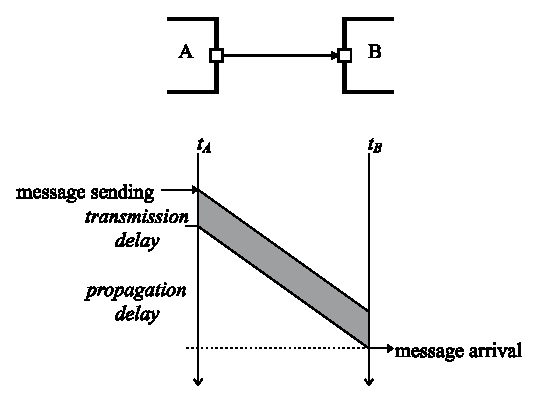
\includegraphics[width=4.301in, height=2.417in]{figures/usmanFig4}
\caption{Message transmission}
\label{fig:ch-overview:message-transm}
\end{center}
\end{figure}

The above model may not be suitable to model all protocols. In Token Ring
and FDDI, stations start to repeat bits before the whole frame arrives;
in other words, frames ``flow through'' the stations, being delayed only a few bits.
In such cases, the data rate modeling feature of {\opp} cannot be used.

If a message travels along a path, passing through successive links and
compound modules, the model behaves as if each module waited until the
last bit of the message arrives and only started its transmission
afterwards.
(Fig. \ref{fig:ch-overview:msg-multiple-ch}).

\begin{figure}[htbp]
\begin{center}
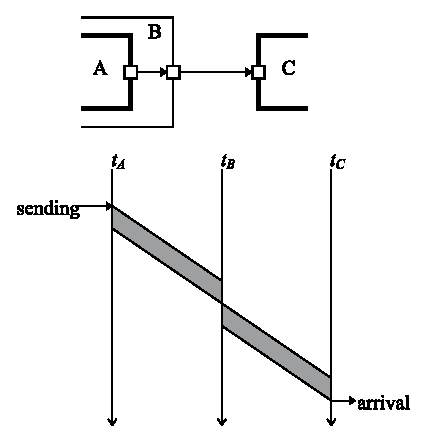
\includegraphics[width=3.330in, height=2.692in]{figures/usmanFig5}
\caption{Message sending over multiple channels}
\label{fig:ch-overview:msg-multiple-ch}
\end{center}
\end{figure}

Since the above effect is usually not the desired one, typically
you will want to assign data rate to only one connection in the
path.


\subsection{Multiple transmissions on links}

If a data rate\index{data rate} is specified for a connection, a message
will have a certain nonzero transmission time\index{transmission
  time}, depending on the length of the connection. This implies that
a message that is passsing through an output gate, ``reserves'' the gate
for a given period (``it is being transmitted'').

\begin{figure}[htbp]
  \begin{center}
    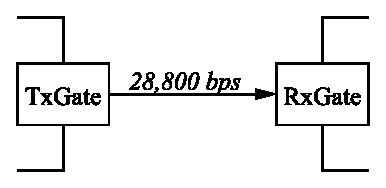
\includegraphics[width=2.315in, height=1.015in]{figures/usmanFig9}
    \caption{Connection with a data rate}
    \label{fig:ch-simple-modules:conn-w-data-rate}
  \end{center}
\end{figure}

While a message is under transmission, other messages have to wait
until the transmission is completed. The module sends another message while the
gate is busy, a runtime error will be thrown.

The {\opp} class library provides functions to check
whether a certain output gate is transmitting and find out when when
it finishes transmission.

If the connection with a data rate is not directly connected
to the simple module's output gate but is the second
one in the path, you have to check the second gate's busy
condition\index{gate!busy condition}.

\begin{note}
   In \opp versions prior to 4.0, sending on a busy gate was permitted, and
   messages got implicitly queued up. The behaviour of the simulation kernel
   was changed because in practice, sending on a busy gate was more often result
   of a programming error than calculated behaviour.
\end{note}


\subsubsection{Implementation of message sending}

Message sending is implemented like this: the arrival time\index{arrival time}
and the bit error\index{bit error} flag of a message are calculated right inside
the \fname{send()} call, then the message gets inserted into the FES\index{FES}
with the calculated arrival time. The message does \textit{not} get scheduled
individually for each link. This implementation was chosen because of its
run-time efficiency.

\begin{note}
   The consequence of this implementation is that any change in the
   channel's parameters (delay, bit rate, bit error rate) will only affect
   messages \textit{sent} after the change. Messages already under way will not
   be influenced by the change.

   This is not a huge problem in practice, but if it is important to model
   channels with changing parameters, the solution is to insert simple modules
   into the path to ensure strict scheduling.
\end{note}


\subsubsection{The approach of some other simulators}

Note that some simulators (e.g. OPNET) assign \textit{packet queues}
to input gates (ports), and messages sent are buffered at the
destination module (or the remote end of the link) until they are
received by the destination module. With that approach, events and
messages are separate entities, that is, a \textit{send} operation
includes placing the message in the packet queue \textit{and} scheduling
an event, which signals the arrival of the packet. In some implementations,
output gates also have packet queues where packets will be buffered until
the channel is ready (available for transmission).

{\opp} gates\index{gate} don't have associated queues. The place
where sent but not yet received messages are buffered in the
FES\index{FES}.  {\opp}'s approach is potentially faster
than the solution mentioned above because it doesn't have the
enqueue/dequeue overhead and also spares an event creation. The
drawback is, that changes to channel parameters do not take effect
immediately.

In {\opp} one can implement \textit{point-to-point transmitter} modules
with packet queues if needed. For example, the INET Framework
follows this approach.




\section{Defining simple module types}

\subsection{Overview}

As mentioned before \ref{sec:simple-modules-in-opp}, a simple module\index{module!simple}
is nothing more than a C++ class which has to be subclassed from
\cclass{cSimpleModule}, with one or more virtual member functions redefined
to define its behavior.

The class has to be registered with {\opp} via the \fmac{Define\_Module()} macro.
The \fmac{Define\_Module()} line should always be put into \ttt{.cc} or \ttt{.cpp}
files and not header file (\ttt{.h}), because the compiler generates code from it.
      \footnote{For completeness, there is also a \fmac{Define\_Module\_Like()}
                macro, but its use is discouraged and might even be removed in
                future {\opp} releases.}

The following \ttt{HelloModule} is about the simplest simple module one could write.
(We could have left out the \ttt{initialize()} method as well to make it even smaller,
but how would it say Hello then?) Note \cclass{cSimpleModule} as base class,
and the \fmac{Define\_Module()} line.

\begin{verbatim}
// file: HelloModule.cc
#include <omnetpp.h>

class HelloModule : public cSimpleModule
{
  protected:
    virtual void initialize();
    virtual void handleMessage(cMessage *msg);
};

// register module class with OMNeT++
Define_Module(HelloModule);

void HelloModule::initialize()
{
    ev << "Hello World!\n";
}

void HelloModule::handleMessage(cMessage *msg)
{
    delete msg; // just discard everything we receive
}
\end{verbatim}

In order to be able to refer to this simple\index{module!simple} module type
in NED files, we also need an associated NED declaration which might
look like this:

\begin{Verbatim}[commandchars=\\\{\}]
// file: HelloModule.ned
\textbf{simple} HelloModule
    \textbf{gates}:
        \textbf{in:} in;
\textbf{endsimple}
\end{Verbatim}


\subsection{Constructor}

Simple modules are never instantiated by the user directly, but rather by
the simulation kernel. This implies that one cannot write arbitrary
constructors: the signature must be what is expected by the simulation kernel.
Luckily, this contract is very simple: the constructor must be public, and must take
no arguments:

\begin{verbatim}
  public:
    HelloModule();  // constructor takes no arguments
\end{verbatim}

\cclass{cSimpleModule} itself has two constructors:
\begin{enumerate}
  \item{\ttt{cSimpleModule()} -- one without arguments}
  \item{\ttt{cSimpleModule(size\_t stacksize)} -- one that accepts the coroutine
        stack size\index{module!stack size}\index{stack!size}}
\end{enumerate}

The first version should be used with \fname{handleMessage()} simple modules,
and the second one with \fname{activity()} modules.
(With the latter, the \fname{activity()} method of the module class
runs as a coroutine\index{coroutine} which needs a separate CPU stack,
usually of 16..32K. This will be discussed in detail later.)
Passing zero stack size to the latter constructor also selects \ttt{handleMessage()}.

Thus, the following constructor definitions are all OK, and select
\fname{handleMessage()} to be used with the module:

\begin{verbatim}
HelloModule::HelloModule() {...}
HelloModule::HelloModule() : cSimpleModule() {...}
\end{verbatim}

It is also OK to omit the constructor altogether, because the
compiler-generated one is suitable too.

The following constructor definition selects \fname{activity()} to be used
with the module, with 16K of coroutine stack:

\begin{verbatim}
HelloModule::HelloModule() : cSimpleModule(16384) {...}
\end{verbatim}

\begin{note}
    The \fmac{Module\_Class\_Members()} macro, already deprecated in \opp 3.2,
    has been removed in the 4.0 version. When porting older simulation models,
    occurrences of this macro can simply be removed from the source code.
\end{note}



\subsection{Constructor and destructor vs initialize() and finish()}

The \fname{initialize()} and \fname{finish()} methods will be discussed
in a later section in detail, but because their apparent similarity
to the constructor and the destructor is prone to cause some confusion,
we'll briefly cover them here.

The constructor gets called when the module is created, as part of the
model setup process. At that time, everything is just being built,
so there isn't a lot things one can do from the constructor.
In contrast, \fname{initialize()} gets called just before the
simulation starts executing, when everything else has been set up
already.

\fname{finish()} is for recording statistics, and it only gets called
when the simulation has terminated normally. It does not get called when
the simulations stops with an error message. The destructor always
gets called at the end, no matter how the simulation stopped, but
at that time it is fair to assume that the simulation model has been
halfway demolished already.

Based on the above, the following conventions exist for these four methods:

\begin{description}

\item Constructor:

Set pointer members of the module class to \ttt{NULL}; postpone all other
initialization tasks to \fname{initialize()}.

\item \fname{initialize()}:

Perform all initialization tasks: read module parameters, initialize
class variables, allocate dynamic data structures with \ttt{new};
also allocate and initialize self-messages (timers) if needed.

\item \fname{finish()}:

Record statistics. Do \tbf{not} \ttt{delete} anything or cancel timers --
all cleanup must be done in the destructor.

\item Destructor:

Delete everything which was allocated by \ttt{new} and is still held
by the module class. With self-messages (timers), use the
\fname{cancelAndDelete(msg)} function! It is almost always wrong
to just delete a self-message from the destructor, because it might be
in the scheduled events list. The \fname{cancelAndDelete(msg)} function
checks for that first, and cancels the message before deletion if necessary.

\end{description}


\subsection{"Garbage collection" and compatibility}
\label{sec:garbage-collection}

{\opp} versions before the 3.2 release had a feature which often was,
informally and also somewhat incorrectly, called \textit{"garbage
collection"} (GC). The purpose of this feature was to mitigate the need for
writing destructors, and often constructors as well by providing automatic
cleanup at the end of the simulation. (It did not do anything during
simulation, as the name might suggest.)

{\opp} (all versions) keep track of user-allocated simulation objects
(typically: messages) and their ownerships. What the \textit{"garbage
collection"} feature did was that during the cleanup of the model, after
each module destructor finished, it checked whether there were simulations
objects left that were apparently owned by that module but not deallocated
by the destructor -- and if it found such objects, it invoked \ttt{delete}
on them.

It worked out nicely in 90 percent of cases, but occasionally it resulted
in spurious crashes which were hard to debug for users not familiar
with {\opp} internals or lacking advanced C++ skills.
    \footnote{These crashes occurred due to lack of information available
              to the GC mechanism, e.g. C++ provides no way to detect
              from the pointer whether an object is part of an array, or is
              inside a struct or class. The solution was to use pointers:
              pointer array, pointer as class member, etc.}

Starting from {\opp} 3.2, this cleanup-time GC mechanism has been disabled by default
(\ttt{perform-gc=} configuration option, see \ref{sec:ch-run-sim:general-section}),
and it generally not recommended to turn it back on. It does not do any harm
to run any simulation model without GC (apart from the memory leak).

It is expected that existing modules will be updated sooner or later, by adding
proper constructors and destructors. To catalyse this process, {\opp} dumps the
list of unreleased objects at the end of the simulation. This dump can also be
turned off in the configuration (\ttt{print-undisposed=} configuration option,
see \ref{sec:ch-run-sim:general-section}).



\subsection{An example}

The following code is a bit longer but actually useful simple module
implementation. It demonstrates several of the above concepts, plus
some others which will be explained in later sections:
\begin{enumerate}
  \item{constructor, initialize and destructor conventions}
  \item{using messages for timers}
  \item{accessing module parameters}
  \item{recording statistics at the end of the simulation}
  \item{documenting the programmer's assumptions using ASSERT()}
\end{enumerate}

\begin{verbatim}
// file: FFGenerator.h

#include <omnetpp.h>

/**
 * Generates messages or jobs; see NED file for more info.
 */
class FFGenerator : public cSimpleModule
{
  private:
    cMessage *sendMessageEvent;
    long numSent;

  public:
    FFGenerator();
    virtual ~FFGenerator();

  protected:
    virtual void initialize();
    virtual void handleMessage(cMessage *msg);
    virtual void finish();
};
\end{verbatim}

\begin{verbatim}
// file: FFGenerator.cc

#include "FFGenerator.cc"

// register module class with OMNeT++
Define_Module(FFGenerator);

FFGenerator::FFGenerator()
{
    sendMessageEvent = NULL;
}

void FFGenerator::initialize()
{
    numSent = 0;
    sendMessageEvent = new cMessage("sendMessageEvent");
    scheduleAt(0.0, sendMessageEvent);
}

void FFGenerator::handleMessage(cMessage *msg)
{
    ASSERT(msg==sendMessageEvent);

    cMessage *m = new cMessage("packet");
    m->setBitLength(par("msgLength"));
    send(m, "out");
    numSent++;

    double deltaT = (double)par("sendIaTime");
    scheduleAt(simTime()+deltaT, sendMessageEvent);
}

void FFGenerator::finish()
{
    recordScalar("packets sent", numSent);
}

FFGenerator::~FFGenerator()
{
    cancelAndDelete(sendMessageEvent);
}
\end{verbatim}

The corresponding NED declaration:

\begin{Verbatim}[commandchars=\\\{\}]
// file: FFGenerator.ned
\textbf{simple} FFGenerator
\{
    \textbf{parameters}:
        \textbf{volatile double} sendIaTime;
    \textbf{gates}:
        \textbf{output} out;
\}
\end{Verbatim}




\subsection{Using global variables}
\index{global variables}

If possible, avoid using global variables, including
static class members. They are prone to cause several problems.
First, they are not reset to their initial values (to zero)
when you rebuild the simulation in Tkenv, or start another run
in Cmdenv. This may produce surprising results.
Second, they prevent you from running your simulation in parallel.
When using parallel simulation, each partition of your model
(may) run in a separate process, having its own copy of the
global variables. This is usually not what you want.

The solution is to encapsulate the variables into simple modules
as private or protected data members, and expose them via public methods.
Other modules can then call these public methods to get or set the values.
Calling methods of other modules will be discussed in section
\ref{ch:simple-modules:direct-method-calls}.
Examples of such modules are the \ttt{Blackboard} in the \textit{Mobility Framework},
and \ttt{InterfaceTable} and \ttt{RoutingTable} in the \textit{INET Framework}.



\section{Adding functionality to cSimpleModule}

This section discusses \cclass{cSimpleModule}'s four previously
mentioned member functions, intended to be redefined by the user:
\fname{initialize()}, \fname{handleMessage()}, \fname{activity()}
and \fname{finish()}, plus a fifth, less frequently used one,
\fname{handleParameterChange}.



\subsection{handleMessage()}

\subsubsection{Function called for each event}


The idea is that at each event\index{event} (message arrival) we
simply call a user-defined function. This function,
\ttt{handleMessage(cMessage *msg)} is a
virtual member function of \cclass{cSimpleModule} which does
nothing by default -- the user has to redefine it in subclasses
and add the message processing code.

The \fname{handleMessage()} function will be called for every message
that arrives at the module. The function should process the message
and return immediately after that. The simulation time is potentially
different in each call. No simulation time elapses within a call
to \fname{handleMessage()}.

The event loop inside the simulator handles both \fname{activity()}
and \fname{handleMessage()} simple modules, and it corresponds
to the following pseudocode:

\begin{Verbatim}[commandchars=\\\{\}]
\textit{while (FES not empty and simulation not yet complete)}
\{
    retrieve first event from FES
    t:= timestamp of this event
    m:= module containing this event
    if (m works with handleMessage())
        \textbf{m->handleMessage( event )}
    else // m works with activity()
        transferTo( m )
\}
\end{Verbatim}

Modules with \fname{handleMessage()} are NOT started automatically:
the simulation kernel creates starter messages\index{starter messages}
only for modules with \fname{activity()}. This means that you have to
schedule self-messages\index{self-message} from the
\fname{initialize()} function if you want a \fname{handleMessage()}
simple module to start working ``by itself'', without first receiving
a message from other modules.


\subsubsection{Programming with handleMessage()}


To use the \fname{handleMessage()} mechanism in a
simple module, you must specify \textit{zero
  stack size}\index{zero stack size} for the module. This is
important, because this tells {\opp} that you want to use
\fname{handleMessage()} and not \fname{activity()}.

Message/event related functions you can use in \fname{handleMessage()}:

\begin{itemize}
  \item{\fname{send()} family of functions -- to send messages to other modules}
  \item{\fname{scheduleAt()} -- to schedule an event (the module ``sends a message to itself'')}
  \item{\fname{cancelEvent()} -- to delete an event scheduled with \fname{scheduleAt()}}
\end{itemize}

You cannot use the \fname{receive()} family and
\fname{wait()} functions in \fname{handleMessage()}, because they are
coroutine-based by nature, as explained in the section about
\fname{activity()}.

You have to add data members to the module class for every piece
of information you want to preserve. This information cannot
be stored in local variables of \fname{handleMessage()} because they
are destroyed when the function returns. Also, they cannot be
stored in static variables in the function (or the class), because
they would be shared between all instances of the class.


Data members to be added to the module class will typically include
things like:

\begin{itemize}
  \item{state (e.g. IDLE/BUSY, CONN\_DOWN/CONN\_ALIVE/...)}
  \item{other variables which belong to the state of the module: retry
    counts, packet queues, etc.}
  \item{values retrieved/computed once and then stored: values of module
    parameters, gate indices, routing information, etc.}
  \item{pointers of message objects created once and then reused for
    timers, timeouts, etc.}
  \item{variables/objects for statistics collection}
\end{itemize}

You can initialize these variables from the \fname{initialize()}
function.  The constructor\index{module!constructor} is not a very good place
for this purpose, because it is called in the network setup phase when
the model is still under construction, so a lot of information you may
want to use is not yet available.

Another task you have to do in \fname{initialize()} is to schedule
initial event(s)\index{events!initial} which trigger the first call(s)
to \fname{handleMessage()}.  After the first call,
\fname{handleMessage()} must take care to schedule further events for
itself so that the ``chain'' is not broken. Scheduling events is not
necessary if your module only has to react to messages coming from
other modules.

\fname{finish()} is normally used to record statistics information
accumulated in data members of the class at the end of the simulation.


\subsubsection{Application area}


\fname{handleMessage()} is in most cases a better choice than \fname{activity()}:

\begin{enumerate}
  \item{When you expect the module to be used in large simulations,
      involving several thousand modules. In such cases, the module stacks
      required by \fname{activity()} would simply consume too much memory.}
  \item{For modules which maintain little or no state information,
      such as packet sinks, \fname{handleMessage()} is more convenient to program.}
  \item{Other good candidates are modules with a large state space and
      many arbitrary state transition possibilities (i.e. where there
      are many possible subsequent states for any state). Such algorithms
      are difficult to program with \fname{activity()}, or the result is code
      which is better suited for \fname{handleMessage()} (see rule of thumb
      below). Most communication protocols are like this.}
\end{enumerate}


\subsubsection{Example 1: Protocol models}

Models of protocol layers in a communication network tend to have
a common structure on a high level because fundamentally they all have to react
to three types of events: to messages arriving from higher layer protocols
(or apps), to messages arriving from lower layer protocols (from the network),
and to various timers and timeouts (that is, self-messages).

This usually results in the following source code pattern:

\begin{verbatim}
class FooProtocol : public cSimpleModule
{
  protected:
    // state variables
    // ...

    virtual void processMsgFromHigherLayer(cMessage *packet);
    virtual void processMsgFromLowerLayer(FooPacket *packet);
    virtual void processTimer(cMessage *timer);

    virtual void initialize();
    virtual void handleMessage(cMessage *msg);
};

// ...

void FooProtocol::handleMessage(cMessage *msg)
{
    if (msg->isSelfMessage())
        processTimer(msg);
    else if (msg->arrivedOn("fromNetw"))
        processMsgFromLowerLayer(check_and_cast<FooPacket *>(msg));
    else
        processMsgFromHigherLayer(msg);
}
\end{verbatim}

The functions \ttt{processMsgFromHigherLayer()}, \ttt{processMsgFromLowerLayer()}
and \ttt{processTimer()} are then usually split further: there are separate
methods to process separate packet types and separate timers.


\subsubsection{Example 2: Simple traffic generators and sinks}


The code for simple packet generators and sinks programmed with \fname{handleMessage()} might
be as simple as the following pseoudocode:

\begin{verbatim}
PacketGenerator::handleMessage(msg)
{
    create and send out a new packet;
    schedule msg again to trigger next call to handleMessage;
}

PacketSink::handleMessage(msg)
{
    delete msg;
}
\end{verbatim}

Note that \textit{PacketGenerator} will need to redefine \fname{initialize()}
to create \textit{m} and schedule the first event.

The following simple module generates packets with exponential
inter-arrival time. (Some details in the source haven't been
discussed yet, but the code is probably understandable nevertheless.)


\begin{Verbatim}[commandchars=\\\{\}]
class Generator : public cSimpleModule
\{
  public:
    Generator() : cSimpleModule() {}
  protected:
    virtual void initialize();
    virtual void handleMessage(cMessage *msg);
\};

Define_Module(Generator);

void Generator::initialize()
\{
    // schedule first sending
    scheduleAt(simTime(), new cMessage);
\}

void Generator::handleMessage(cMessage *msg)
\{
    // generate & send packet
    cMessage *pkt = new cMessage;
    send(pkt, "out");
    // schedule next call
    scheduleAt(simTime()+exponential(1.0), msg);
\}
\end{Verbatim}



\subsubsection{Example 3: Bursty traffic generator}


A bit more realistic example is to rewrite our Generator to create
packet bursts, each consisting of \ttt{burstLength} packets.

We add some data members to the class:
\begin{itemize}
\item{\ttt{burstLength} will store the parameter that specifies how many
    packets a burst must contain,}
\item{\ttt{burstCounter} will count in how many packets are left to be sent
    in the current burst.}
\end{itemize}

The code:

\begin{Verbatim}[commandchars=\\\{\}]
class BurstyGenerator : public cSimpleModule
\{
  protected:
    int burstLength;
    int burstCounter;

    virtual void initialize();
    virtual void handleMessage(cMessage *msg);
\};

Define_Module(BurstyGenerator);

void BurstyGenerator::initialize()
\{
    // init parameters and state variables
    burstLength = par("burstLength");
    burstCounter = burstLength;
    // schedule first packet of first burst
    scheduleAt(simTime(), new cMessage);
\}

void BurstyGenerator::handleMessage(cMessage *msg)
\{
    // generate & send packet
    cMessage *pkt = new cMessage;
    send(pkt, "out");
    // if this was the last packet of the burst
    if (--burstCounter == 0)
    \{
        // schedule next burst
        burstCounter = burstLength;
        scheduleAt(simTime()+exponential(5.0), msg);
    \}
    else
    \{
        // schedule next sending within burst
        scheduleAt(simTime()+exponential(1.0), msg);
    \}
\}
\end{Verbatim}



\subsubsection{Pros and Cons of using \fname{handleMessage()}}


Pros:
\begin{itemize}
  \item{consumes less memory: no separate stack needed for simple modules}
  \item{fast: function call is faster than switching between coroutines\index{coroutine}}
\end{itemize}

Cons:
\begin{itemize}
  \item{local variables cannot be used to store state information}
  \item{need to redefine \fname{initialize()}}
\end{itemize}

Usually, \fname{handleMessage()} should be preferred to \fname{activity()}.


\subsubsection{Other simulators}


Many simulation packages use a similar approach, often topped with
something like a state machine\index{finite state machine}
(FSM\index{FSM}) which hides the underlying function calls. Such
systems are:
\begin{itemize}
  \item{OPNET$^TM$ which uses FSM's designed using a graphical editor;}
  \item{NetSim++ clones OPNET's approach;}
  \item{SMURPH (University of Alberta) defines a (somewhat eclectic)
      language to describe FSMs, and uses a precompiler to turn it
      into C++ code;}
  \item{Ptolemy (UC Berkeley) uses a similar method.}
\end{itemize}

{\opp}'s FSM\index{FSM} support is described in the next section.



\subsection{activity()}

\subsubsection{Process-style description}

With \fname{activity()}, you can code the simple
module much like you would code an operating system process or a
thread. You can wait for an incoming message (event) at any point of
the code, you can suspend the execution for some time (model time!),
etc. When the \fname{activity()} function exits, the module is
terminated.  (The simulation can continue if there are other modules
which can run.)


The most important functions you can use in \fname{activity()} are
(they will be discussed in detail later):
\begin{itemize}
\item{\fname{receive()} -- to receive messages (events)}
\item{\fname{wait()} -- to suspend execution\index{suspend execution}
    for some time (model time)}
\item{\fname{send()} family of functions -- to send messages to other
    modules}
\item{\fname{scheduleAt()} -- to schedule an event (the module ``sends
    a message to itself'')}
\item{\fname{cancelEvent()} -- to delete an event scheduled with
    scheduleAt()}
\item{\fname{end()} -- to finish execution of this module (same as
    exiting the \fname{activity()} function)}
\end{itemize}

The \fname{activity()} function normally contains an infinite loop,
with at least a \fname{wait()} or \fname{receive()} call in its body.



\subsubsection{Application area}

Generally you should prefer \ttt{handleMessage()} to \ttt{activity()}.
The main problem with \ttt{activity()} is that it doesn't scale because
every module needs a separate coroutine stack. It has also been observed
that \ttt{activity()} does not encourage a good programming style.

There is one scenario where \ttt{activity()}'s process-style
description is convenient: when the process has many
states but transitions are very limited, ie. from any state the
process can only go to one or two other states.  For example, this is
the case when programming a network application, which uses a single
network connection.  The pseudocode of the application which talks to
a transport layer protocol might look like this:

\begin{Verbatim}[commandchars=\\\{\}]
\textit{activity()}
\{
    while(true)
    \{
        open connection by sending OPEN command to transport layer
        receive reply from transport layer
        if (open not successful)
        \{
            wait(some time)
            continue // loop back to while()
        \}

        while(there's more to do)
        \{
            send data on network connection
            if (connection broken)
            \{
                continue outer loop // loop back to outer while()
            \}
            wait(some time)
            receive data on network connection
            if (connection broken)
            \{
                continue outer loop // loop back to outer while()
            \}
            wait(some time)
        \}
        close connection by sending CLOSE command to transport layer
        if (close not successful)
        \{
            // handle error
        \}
        wait(some time)
    \}
\}
\end{Verbatim}

If you have to handle several connections simultaneously, you may
dynamically create them as instances of the simple module above.
Dynamic module creation will be discussed later.

There are situations when you certainly \textit{do not want} to use \fname{activity()}.
If your \fname{activity()} function contains no \fname{wait()} and it has
only one \fname{receive()} call at the top of an infinite loop,
there's no point in using \ttt{activity()} and the code should be written
with \ttt{handleMessage()}.
The body of the infinite loop would then become the body to \fname{handleMessage()},
state variables inside \fname{activity()} would become data members in
the module class, and you'd initialize them in \fname{initialize()}.

Example:

\begin{verbatim}
void Sink::activity()
{
    while(true)
    {
        msg = receive();
        delete msg;
    }
}
\end{verbatim}

should rather be programmed as:

\begin{verbatim}
void Sink::handleMessage(cMessage *msg)
{
    delete msg;
}
\end{verbatim}



\subsubsection{Activity() is run as a coroutine}


\fname{activity()} is run in a coroutine\index{coroutine}.
Coroutines are a sort of threads which are scheduled
non-preemptively (this is also called cooperative
multitasking\index{multitasking!cooperative}). From one coroutine you
can switch to another coroutine by a
\ttt{transferTo(otherCoroutine)} call. Then this
coroutine is suspended and \textit{otherCoroutine} will run. Later,
when \textit{otherCoroutine} does a
\ttt{transferTo(firstCoroutine)} call, execution of
the first coroutine will resume from the point of the
\ttt{transferTo(otherCoroutine)} call.  The full state
of the coroutine, including local variables are preserved while the
thread of execution is in other coroutines.  This implies that each
coroutine must have its own processor stack\index{stack}, and
\fname{transferTo()} involves a switch from one processor stack to
another.


Coroutines\index{coroutine} are at the heart of {\opp}, and the
simulation programmer doesn't ever need to call \fname{transferTo()}
or other functions in the coroutine library, nor does he need to care
about the coroutine library implementation. It is important to
understand, however, how the event loop found in discrete event simulators
works with coroutines.


When using coroutines, the event loop\index{event loop} looks like
this (simplified):


\begin{Verbatim}[commandchars=\\\{\}]
\textit{while (FES not empty and simulation not yet complete)}
\{
    retrieve first event from FES
    t:= timestamp of this event
    \textbf{transferTo(module containing the event)}
\}
\end{Verbatim}



That is, when the module has an event\index{event}, the simulation
kernel transfers the control to the module's coroutine. It is expected
that when the module ``decides it has finished the processing of the
event'', it will transfer the control back to the simulation kernel by
a \ttt{transferTo(main)} call. Initially,
simple\index{module!simple} modules using \fname{activity()} are
``booted'' by events (\textit{''starter messages''}\index{starter messages})
inserted into the FES\index{FES} by the simulation kernel before the
start of the simulation.


How does the coroutine know it has ``finished processing the event''?
The answer: \textit{when it requests another event}.  The functions
which request events from the simulation kernel are the
\fname{receive()} and \fname{wait()}, so their
implementations contain a \ttt{transferTo(main)} call
somewhere.


Their pseudocode, as implemented in {\opp}:


\begin{Verbatim}[commandchars=\\\{\}]
receive()
\{
    transferTo(main)
    retrieve current event
    return the event // remember: events = messages
\}

wait()
\{
    create event e
    schedule it at (current sim. time + wait interval)
    transferTo(main)
    retrieve current event
    if (current event is not e) \{
        error
    \}
    delete e  // note: actual impl. reuses events
    return
\}
\end{Verbatim}



Thus, the \fname{receive()} and \fname{wait()} calls are
special points in the \fname{activity()} function, because
they are where

\begin{itemize}
  \item{simulation time elapses in the module, and}
  \item{other modules get a chance to execute.}
\end{itemize}


\subsubsection{Starter messages}


Modules written with \fname{activity()} need starter
messages\index{starter messages} to ``boot''.  These starter messages
are inserted into the FES\index{FES} automatically by {\opp} at the
beginning of the simulation, even before the \fname{initialize()}
functions are called.


\subsubsection{Coroutine stack size}


The simulation programmer needs to define the processor stack size\index{coroutine!stack size}
for coroutines. This cannot be automated.

16 or 32 kbytes is usually a good choice, but you may need more if the
module uses recursive functions or has local variables, which occupy a
lot of stack space. {\opp} has a built-in mechanism that will usually
detect if the module stack is too small and overflows\index{stack!overflow}.
{\opp} can also tell you how much stack space a module actually uses\index{stack!usage},
so you can find out if you overestimated the stack needs.


\subsubsection{initialize() and finish() with activity()}


Because local variables of \fname{activity()} are preserved across
events, you can store everything (state information, packet buffers,
etc.) in them. Local variables can be initialized at the top of the
\fname{activity()} function, so there isn't much need to use
\fname{initialize()}.


You do need \fname{finish()}, however, if you want to write statistics at
the end of the simulation. Because \fname{finish()} cannot access
the local variables of \fname{activity()}, you have to put the variables
and objects containing the statistics into the module class.
You still don't need \fname{initialize()} because class members can also
be initialized at the top of \fname{activity()}.


Thus, a typical setup looks like this in pseudocode:


\begin{Verbatim}[commandchars=\\\{\}]
\textit{class MySimpleModule...}
\{
    ...
    variables for statistics collection
    activity();
    finish();
\};

MySimpleModule::activity()
\{
    declare local vars and initialize them
    initialize statistics collection variables

    while(true)
    \{
        ...
    \}
\}

MySimpleModule::finish()
\{
    record statistics into file
\}
\end{Verbatim}


\subsubsection{Pros and Cons of using \fname{activity()}}


Pros:
\begin{itemize}
   \item{\fname{initialize()} not needed, state can be stored in local
       variables of \fname{activity()}}
   \item{process-style description is a natural programming model in some cases}
\end{itemize}

Cons:
\begin{itemize}
   \item{limited scalability: coroutine stacks can unacceptably increase the
       memory requirements of the simulation program if you have several
       thousands or ten thousands of simple modules;}
   \item{run-time overhead: switching between coroutines is somewhat slower
       than a simple function call}
   \item{does not enforce a good programming style: using \ttt{activity()}
       tends to lead to unreliable, spaghetti code}
\end{itemize}

In most cases, cons outweigh pros and it is a better idea to use
\ttt{handleMessage()} instead.


\subsubsection{Other simulators}


Coroutines are used by a number of other simulation packages:
\begin{itemize}
\item{All simulation software which inherits from SIMULA (e.g. C++SIM)
    is based on coroutines, although all in all the programming
    model is quite different.}
\item{The simulation/parallel programming language Maisie and its successor
    PARSEC (from UCLA) also use coroutines (although implemented
    with ``normal'' preemptive threads). The philosophy
    is quite similar to {\opp}. PARSEC, being ``just''
    a programming language, it has a more elegant syntax but far fewer
    features than {\opp}.}
\item{Many Java-based simulation libraries are based on Java
    threads.}
\end{itemize}




\subsection{initialize() and finish()}

\subsubsection{Purpose}


\fname{initialize()} -- to provide place for any user setup code

\fname{finish()} -- to provide place where the user can record statistics
after the simulation has completed


\subsubsection{When and how they are called}


The \fname{initialize()} functions of the modules are invoked
\textit{before} the first event is processed, but \textit{after} the
initial events (starter messages\index{starter messages}) have been
placed into the FES\index{FES} by the simulation kernel.


Both simple and compound modules have \fname{initialize()} functions.
A compound module's \fname{initialize()} function runs
\textit{before} that of its submodules.


The \fname{finish()} functions are called when the event
loop\index{event loop} has terminated, and only if it terminated
normally (i.e. not with a runtime error).  The calling order is the
reverse of the order of \fname{initialize()}: first submodules, then the
encompassing compound module. (The bottom line is that at the moment
there is no ``official'' possibility to redefine \fname{initialize()}
and \fname{finish()} for compound modules; the unofficial way is to
write into the nedtool-generated C++ code. Future versions of {\opp} will
support adding these functions to compound modules.)

This is summarized in the following pseudocode:


\begin{Verbatim}[commandchars=\\\{\}]
\textit{perform simulation run:}
    build network
      (i.e. the system module and its submodules recursively)
    insert starter messages for all submodules using activity()
    do callInitialize() on system module
        \textit{enter event loop // (described earlier)}
    if (event loop terminated normally) // i.e. no errors
        do callFinish() on system module
    clean up

callInitialize()
\{
    call to user-defined initialize() function
    if (module is compound)
        for (each submodule)
            do callInitialize() on submodule
\}

callFinish()
\{
    if (module is compound)
        for (each submodule)
            do callFinish() on submodule
    call to user-defined finish() function
\}
\end{Verbatim}



\subsubsection{initialize() vs. constructor}


Usually you should not put simulation-related code into the
simple module constructor\index{module!constructor}. This is because
modules often need to investigate their surroundings (maybe
the whole network) at the beginning of the simulation and save the
collected info into internal tables.  Code like that cannot be placed
into the constructor since the network is still being set up when the
constructor is called.


\subsubsection{finish() vs. destructor}


Keep in mind that \fname{finish()} is not always called, so it isn't a
good place for cleanup code which should run every time the module is
deleted. \fname{finish()} is only a good place for writing statistics,
result post-processing and other operations  which are supposed to run only on
successful completion. Cleanup code should go into the
destructor\index{module!destructor}.


\subsubsection{Multi-stage initialization}


In simulation models, when one-stage
initialization\index{initialization} provided by \fname{initialize()}
is not sufficient, one can use multi-stage
initialization\index{initialization!multi-stage}.  Modules have two
functions which can be redefined by the user:

\begin{verbatim}
void initialize(int stage);
int numInitStages() const;
\end{verbatim}

At the beginning of the simulation, \ttt{initialize(0)}
is called for \textit{all} modules, then \ttt{initialize(1)},
\ttt{initialize(2)}, etc. You can think of it like
initialization takes place in several ``waves''. For each module,
\fname{numInitStages()} must be redefined to return the number of init
stages required, e.g. for a two-stage init, \fname{numInitStages()}
should return 2, and \fname{initialize(int stage)} must be implemented to
handle the \textit{stage=0} and \textit{stage=1} cases.
  \footnote{Note \ttt{const} in the \ttt{numInitStages()} declaration.
  If you forget it, by C++ rules you create a \textit{different} function
  instead of redefining the existing one in the base class, thus the
  existing one will remain in effect and return 1.}

The \fname{callInitialize()} function performs the full multi-stage initialization
for that module and all its submodules.

If you do not redefine the multi-stage initialization functions, the
default behavior is single-stage initialization: the default
\fname{numInitStages()} returns 1, and the default \ttt{initialize(int stage)}
simply calls \fname{initialize()}.


\subsubsection{``End-of-Simulation'' event}


The task of \fname{finish()} is solved in several simulators
by introducing a special \textit{end-of-simulation}\index{end-of-simulation} event.
This is not a very good practice because the simulation programmer has to
code the models (often represented as FSMs) so that they can \textit{always}
properly respond to end-of-simulation events, in whichever state they are. This
often makes program code unnecessarily complicated.

This can also be witnessed in the design of the PARSEC\index{PARSEC}
simulation language (UCLA). Its predecessor Maisie used
end-of-simulation events, but -- as documented in the PARSEC manual --
this has led to awkward programming in many cases, so for PARSEC
end-of-simulation events were dropped in favour of \fname{finish()}
(called \fname{finalize()} in PARSEC).


\subsection{handleParameterChange()}

The \fname{handleParameterChange()} method was added in {\opp} 3.2,
and it gets called by the simulation kernel when a module parameter changes.
The method signature is the following:

\begin{verbatim}
void handleParameterChange(const char *parname);
\end{verbatim}

The user can redefine this method to let the module react to runtime parameter
changes. A typical use is to re-read the changed parameter, and update
the module state if needed. For example, if a timeout value changes,
one can restart or modify running timers.

The primary motivation for this functionality was to facilitate
the implementation of \textit{scenario manager} modules which
can be programmed to change parameters at certain simulation times.
Such modules can be very convenient in studies involving transient behaviour.

The following example shows a queue module, which supports
runtime change of its \ttt{serviceTime} parameter:

\begin{verbatim}
void Queue::handleParameterChange(const char *parname)
{
    if (strcmp(parname, "serviceTime")==0)
    {
        // queue service time parameter changed, re-read it
        serviceTime = par("serviceTime");

        // if there any job being serviced, modify its service time
        if (endServiceMsg->isScheduled())
        {
            cancelEvent(endServiceMsg);
            scheduleAt(simTime()+serviceTime, endServiceMsg);
        }
    }
}
\end{verbatim}




\subsection{Reusing module code via subclassing}

It is often needed to have several variants of a simple module.
A good design strategy is to create a simple module class with
the common functionality, then subclass from it to create the
specific simple module types.

% FIXME use QueueBase example!

An example:

\begin{verbatim}
class ModifiedTransportProtocol : public TransportProtocol
{
  protected:
    virtual void recalculateTimeout();
};

Define_Module(ModifiedTransportProtocol);

void ModifiedTransportProtocol::recalculateTimeout()
{
    //...
}
\end{verbatim}


\section{Finite State Machines in {\opp}}

\subsubsection{Overview}


Finite State Machines\index{finite state machine} (FSMs)\index{FSM}
can make life with \fname{handleMessage()} easier. {\opp} provides a
class and a set of macros to build FSMs. {\opp}'s FSMs work very much
like OPNET's or SDL's.


The key points are:
\begin{itemize}
\item{There are two kinds of states:
    \textit{transient}\index{transient states} and
    \textit{steady}\index{steady states}. At each event (that is, at
    each call to \fname{handleMessage()}), the FSM transitions out of
    the current (\textit{steady}) state, undergoes a series of state
    changes (runs through a number of \textit{transient} states), and
    finally arrives at another \textit{steady} state. Thus between two
    events, the system is always in one of the steady states.
    Transient states are therefore not really a must -- they exist
    only to group actions to be taken during a transition in a
    convenient way.}
\item{You can assign program code to handle entering and leaving a state
    (known as entry/exit code)\index{entry code}\index{exit code}.
    Staying in the same state is handled as leaving and re-entering
    the state.}
\item{Entry code should not modify the state (this is verified by
    {\opp}).  State changes (transitions) must be put into the exit
    code.}
\end{itemize}

{\opp}'s FSMs \textit{can} be nested\index{FSM!nested}. This means
that any state (or rather, its entry or exit code) may contain a
further full-fledged \fmac{FSM\_Switch()} (see below). This allows you
to introduce sub-states and thereby bring some structure into the
state space if it would become too large.


\subsubsection{The FSM API}


FSM state is stored in an object of type \cclass{cFSM}. The possible states
are defined by an enum; the enum is also a place to define, which
state is transient and which is steady. In the following example, SLEEP
and ACTIVE are steady states and SEND is transient (the numbers
in parentheses must be unique within the state type and they are used
for constructing the numeric IDs for the states):

\begin{verbatim}
enum {
  INIT = 0,
  SLEEP = FSM_Steady(1),
  ACTIVE = FSM_Steady(2),
  SEND = FSM_Transient(1),
};
\end{verbatim}



The actual FSM is embedded in a switch-like statement,
\fmac{FSM\_Switch()}, where you have cases for entering and leaving
each state:


\begin{Verbatim}[commandchars=\\\{\}]
FSM_Switch(fsm)
\{
  case FSM_Exit(\textit{state1}):
    //...
    break;
  case FSM_Enter(\textit{state1}):
    //...
    break;
  case FSM_Exit(\textit{state2}):
    //...
    break;
  case FSM_Enter(\textit{state2}):
    //...
    break;
  //...
\};
\end{Verbatim}


State transitions\index{state transition} are done via calls to
\fmac{FSM\_Goto()}, which simply stores the new state in the
\cclass{cFSM} object:

\begin{Verbatim}[commandchars=\\\{\}]
FSM_Goto(fsm,\textit{newState});
\end{Verbatim}

The FSM starts from the state with the numeric code 0; this state
is conventionally named INIT.


\subsubsection{Debugging FSMs}

FSMs can log their state transitions \ttt{ev}\index{ev},
with the output looking like this:

\begin{verbatim}
...
FSM GenState: leaving state SLEEP
FSM GenState: entering state ACTIVE
...
FSM GenState: leaving state ACTIVE
FSM GenState: entering state SEND
FSM GenState: leaving state SEND
FSM GenState: entering state ACTIVE
...
FSM GenState: leaving state ACTIVE
FSM GenState: entering state SLEEP
...
\end{verbatim}

To enable the above output, you have to \ttt{\#define FSM\_DEBUG}\index{FSM\_DEBUG}
before including \ttt{omnetpp.h}.

\begin{Verbatim}[commandchars=\\\{\}]
#define FSM_DEBUG    // enables debug output from FSMs
#include <omnetpp.h>
\end{Verbatim}

The actual logging is done via the \fmac{FSM\_Print()} macro.
It is currently defined as follows, but you can change the
output format by undefining \ttt{FSM\_Print()} after including
\ttt{omnetpp.ini} and providing a new definition instead.

\begin{verbatim}
#define FSM_Print(fsm,exiting)
  (ev << "FSM " << (fsm).getName()
      << ((exiting) ? ": leaving state " : ": entering state ")
      << (fsm).getStateName() << endl)
\end{verbatim}


\subsubsection{Implementation}


The \fmac{FSM\_Switch()} is a macro. It expands to a \fname{switch()}
statement embedded in a \fname{for()} loop which repeats until the
FSM\index{FSM} reaches a steady state. (The actual code is rather
scary, but if you're dying to see it, it is in \texttt{cfsm.h}.)

Infinite loops are avoided by counting state transitions: if
an FSM goes through 64 transitions without reaching a steady
state, the simulation will terminate with an error message.


\subsubsection{An example}


Let us write another bursty generator. It will have two
states, SLEEP and ACTIVE. In the SLEEP state, the module does
nothing. In the ACTIVE state, it sends messages with a given
inter-arrival time. The code was taken from the Fifo2 sample
simulation.


\begin{Verbatim}[commandchars=\\\{\}]
#define FSM_DEBUG
#include <omnetpp.h>

class BurstyGenerator : public cSimpleModule
\{
  protected:
    // parameters
    double sleepTimeMean;
    double burstTimeMean;
    double sendIATime;
    cPar *msgLength;

    // FSM and its states
    cFSM fsm;
    enum \{
      INIT = 0,
      SLEEP = FSM_Steady(1),
      ACTIVE = FSM_Steady(2),
      SEND = FSM_Transient(1),
    \};

    // variables used
    int i;
    cMessage *startStopBurst;
    cMessage *sendMessage;

    // the virtual functions
    virtual void initialize();
    virtual void handleMessage(cMessage *msg);
\};

Define_Module(BurstyGenerator);

void BurstyGenerator::initialize()
\{
    fsm.setName("fsm");
    sleepTimeMean = par("sleepTimeMean");
    burstTimeMean = par("burstTimeMean");
    sendIATime = par("sendIATime");
    msgLength = &par("msgLength");
    i = 0;
    WATCH(i); // always put watches in initialize()
    startStopBurst = new cMessage("startStopBurst");
    sendMessage = new cMessage("sendMessage");
    scheduleAt(0.0,startStopBurst);
\}

void BurstyGenerator::handleMessage(cMessage *msg)
\{
  FSM_Switch(fsm)
 \{
    case FSM_Exit(INIT):
      // transition to SLEEP state
      FSM_Goto(fsm,SLEEP);
      break;
    case FSM_Enter(SLEEP):
      // schedule end of sleep period (start of next burst)
      scheduleAt(simTime()+exponential(sleepTimeMean),
                 startStopBurst);
    break;
    case FSM_Exit(SLEEP):
      // schedule end of this burst
      scheduleAt(simTime()+exponential(burstTimeMean),
                 startStopBurst);
      // transition to ACTIVE state:
      if (msg!=startStopBurst) \{
        error("invalid event in state ACTIVE");
      \}
      FSM_Goto(fsm,ACTIVE);
      break;
    case FSM_Enter(ACTIVE):
      // schedule next sending
      scheduleAt(simTime()+exponential(sendIATime), sendMessage);
    break;
    case FSM_Exit(ACTIVE):
      // transition to either SEND or SLEEP
      if (msg==sendMessage) \{
        FSM_Goto(fsm,SEND);
      \} else if (msg==startStopBurst) \{
        cancelEvent(sendMessage);
        FSM_Goto(fsm,SLEEP);
      \} else \{
        error("invalid event in state ACTIVE");
      \}
      break;
    case FSM_Exit(SEND):
    \{
      // generate and send out job
      char msgname[32];
      sprintf( msgname, "job-%d", ++i);
      ev << "Generating " << msgname << endl;
      cMessage *job = new cMessage(msgname);
      job->setBitLength( (long) *msgLength );
      job->setTimestamp();
      send( job, "out" );
      // return to ACTIVE
      FSM_Goto(fsm,ACTIVE);
      break;
    \}
  \}
\}
\end{Verbatim}





\section{Sending and receiving messages}
\label{ch:simple-modules:sending-and-receiving}

On an abstract level, an {\opp} simulation model is a set of
simple modules that communicate with each other via message passing.
The essence of simple modules is that they create, send, receive,
store, modify, schedule and destroy messages -- everything else
is supposed to facilitate this task, and collect statistics
about what was going on.

Messages in {\opp} are instances of the \ttt{cMessage} class or
one of its subclasses. Message objects are created using the C++
\ttt{new} operator and destroyed using the \ttt{delete} operator
when they are no longer needed. During their lifetimes,
messages travel between modules via gates and connections
(or are sent directly, bypassing the connections), or
they are scheduled by and delivered to modules,
representing internal events of that module.

Messages are described in detail in chapter \ref{cha:messages}.
At this point, all we need to know about them is that they are
referred to as \ttt{cMessage *} pointers. Message objects
can be given descriptive names (a \ttt{const char *} string)
that often helps in debugging the simulation. The message
name string can be specified in the constructor, so it
should not surprise you if you see something like
\ttt{new cMessage("token")} in the examples below.



\subsection{Sending messages}

Once created, a message object can be sent through an
output gate\index{output!gate} using one of the following functions:

\begin{verbatim}
send(cMessage *msg, const char *gateName, int index=0);
send(cMessage *msg, int gateId);
send(cMessage *msg, cGate *gate);
\end{verbatim}

In the first function, the argument \ttt{gateName} is the name of
the gate the message has to be sent through. If this gate is
a vector gate, \ttt{index} determines though which particular output
gate this has to be done; otherwise, the \ttt{index} argument is not
needed.

The second and third functions use the gate Id and the pointer to the gate
object. They are faster than the first one because they don't have to
search through the gate array.

Examples:

\begin{verbatim}
send(msg, "outGate");
send(msg, "outGates", i); // send via outGates[i]
\end{verbatim}

The following code example creates and sends messages
every 5 simulated seconds:

\begin{verbatim}
int outGateId = findGate("outGate");
while(true)
{
  send(new cMessage("packet"), outGateId);
  wait(5);
}
\end{verbatim}


\subsubsection{Modeling packet transmissions}

If you're sending messages over a link that has (nonzero) data rate,
it is modeled as described earlier in this manual, in
section \ref{ch:simple-modules:packet-transmission}.

If you want to have full control over the transmission process,
you'll probably need the \fname{isBusy()} and \fname{getTransmissionFinishTime()}
member functions of \cclass{cGate}. They are described in section
\ref{ch:simple-modules:cgate-transmission-state}.



\subsection{Broadcasts and retransmissions}

When you implement broadcasts or retransmissions, two frequently
occurring tasks in protocol simulation, you might feel tempted
to use the same message in multiple \fname{send()} operations.
Do not do it -- you cannot send the same message object multiple times.
The solution in such cases is duplicating the message.

\subsubsection{Broadcasting messages}

In your model, you may need to broadcast a message to several destinations.
Broadcast can be implemented in a simple module by sending out copies
of the same message, for example on every gate of a gate vector.
As described above, you cannot use the same message pointer for
in all \fname{send()} calls -- what you have to do instead is
create copies (duplicates) of the message object and send them.

Example:

\begin{verbatim}
for (int i=0; i<n; i++)
{
    cMessage *copy = (cMessage *) msg->dup();
    send(copy, "out", i);
}
delete msg;
\end{verbatim}

You might have noticed that copying the message for the last gate is
redundant (we could send out the original message),
so it can be optimized out like this:

\begin{verbatim}
for (int i=0; i<n-1; i++)   // note n-1 instead of n
{
    cMessage *copy = (cMessage *) msg->dup();
    send(copy, "out", i);
}
send(msg, "out", n-1);  // send original on last gate
\end{verbatim}


\subsubsection{Retransmissions}

Many communication protocols involve retransmissions of packets (frames).
When implementing retransmissions, you cannot just hold a pointer
to the same message object and send it again and again -- you'd get
the \textit{not owner of message} error on the first resend.

Instead, whenever it comes to (re)transmission, you should create and
send copies of the message, and retain the original.
When you are sure there will not be any more retransmission,
you can delete the original message.

Creating and sending a copy:

\begin{verbatim}
// (re)transmit packet:
cMessage *copy = (cMessage *) packet->dup();
send(copy, "out");
\end{verbatim}

and finally (when no more retransmissions will occur):

\begin{verbatim}
delete packet;
\end{verbatim}


\subsubsection{Why?}

A message is like any real world object -- it cannot be at two places
at the same time. Once you've sent it, the message object
no longer belongs to the module: it is taken over by the simulation kernel,
and will eventually be delivered to the destination module.
The sender module should not even refer to its pointer any more.
Once the message arrived in the destination module, that module
will have full authority over it -- it can send it on,
destroy it immediately, or store it for further handling.
The same applies to messages that have been scheduled -- they
belong to the simulation kernel until they are delivered back to
the module.

To enforce the rules above, all message sending functions
check that you actually own the message you are about to send.
If the message is with another module, it is currently scheduled or
in a queue etc., you'll get a runtime error: \textit{not owner of message}.
  \footnote{The feature does not increase runtime overhead significantly, because
  it uses the object ownership\index{ownership} management (described in
  Section \ref{sec:ch-sim-lib:ownership-management});
  it merely checks that the owner of the message is the module that
  wants to send it.}



\subsection{Delayed sending}

It is often needed to model a delay (processing time, etc.) immediately
followed by message sending. In {\opp}, it is possible to implement
it like this:

\begin{verbatim}
wait( someDelay );
send( msg, "outgate" );
\end{verbatim}


If the module needs to react to messages that arrive during the delay,
\fname{wait()} cannot be used and the timer mechanism described in
Section \ref{sec:ch-simple-modules:self-messages}, ``Self-messages'', would
need to be employed.


There is also a more straightforward method than those mentioned above:
delayed sending\index{delayed sending}. Delayed sending can be achieved
by using one of these functions:

\begin{verbatim}
sendDelayed(cMessage *msg, double delay, const char *gateName, int index);
sendDelayed(cMessage *msg, double delay, int gateId);
sendDelayed(cMessage *msg, double delay, cGate *gate);
\end{verbatim}

The arguments are the same as for \fname{send()}, except for the extra \textit{delay}
parameter. The effect of the function is the same as if the module
had kept the message for the delay interval and sent it afterwards.
That is, the sending time of the message will be the current
simulation time (time at the \fname{sendDelayed()} call) plus the delay.
The delay value must be non-negative.

Example:

\begin{verbatim}
sendDelayed(msg, 0.005, "outGate");
\end{verbatim}



\subsection{Direct message sending}

Sometimes it is necessary or convenient to ignore gates/connections
and send a message directly to a remote destination module. The \fname{sendDirect()}
function does that:

\begin{verbatim}
sendDirect(cMessage *msg, double delay, cModule *mod, int gateId)
sendDirect(cMessage *msg, double delay, cModule *mod, const char *gateName, int index=-1)
sendDirect(cMessage *msg, double delay, cGate *gate)
\end{verbatim}

In addition to the message and a delay, it also takes the destination module
and gate. The gate should be an \textit{input} gate and should not be connected.
In other words, the module needs dedicated gates for receiving via \ttt{sendDirect()}.
(Note: For leaving a gate unconnected in a compound module, you'll need to specify
\ttt{connections nocheck:} instead of plain \ttt{connections:} in the NED file.)

An example:

\begin{verbatim}
cModule *destinationModule = getParentModule()->getSubmodule("node2");
double delay = truncnormal(0.005, 0.0001);
sendDirect(new cMessage("packet"), delay, destinationModule, "inputGate");
\end{verbatim}

At the destination module, there is no difference between messages received
directly and those received over connections.



\subsection{Receiving messages}

\textbf{With activity() only!} The message receiving functions can
only be used in the \fname{activity()} function,
\fname{handleMessage()} gets received messages in its argument list.

Messages are received using the \fname{receive()} function.
\fname{receive()} is a member of \cclass{cSimpleModule}.

\begin{verbatim}
cMessage *msg = receive();
\end{verbatim}

The \fname{receive()} function accepts an optional \textit{timeout}
parameter\index{receive!timeout}. (This is a \textit{delta}, not an
absolute simulation time.) If an appropriate message doesn't arrive
within the timeout period, the function returns a NULL pointer.
    \footnote{Putaside-queue and the functions \ttt{receiveOn()},
    \ttt{receiveNew()}, and \ttt{receiveNewOn()} were deprecated
    in {\opp} 2.3 and removed in {\opp} 3.0.}

\begin{verbatim}
simtime_t timeout = 3.0;
cMessage *msg = receive( timeout );

if (msg==NULL)
{
    ...   // handle timeout
}
else
{
    ...  // process message
}
\end{verbatim}



\subsection{The wait() function}

\textbf{With activity() only!} The \fname{wait()} function's implementation
contains a \fname{receive()} call which cannot be used in \fname{handleMessage()}.

The \fname{wait()} function suspends the execution of the module for
a given amount of simulation time (a \textit{delta}).

\begin{verbatim}
wait( delay );
\end{verbatim}

In other simulation software, \fname{wait()} is often called \textit{hold}.
Internally, the \fname{wait()} function is implemented by a
\fname{scheduleAt()} followed by a \fname{receive()}.
The \fname{wait()} function is very convenient in modules that do not need
to be prepared for arriving messages, for example message generators.
An example:

\begin{verbatim}
for(;;)
{
  // wait for a (potentially random amount of) time, specified
  // in the interArrivalTime module parameter
  wait( par("interArrivalTime") );

  // generate and send message
  ...
}
\end{verbatim}

It is a runtime error if a message arrives during the wait interval.
If you expect messages to arrive during the wait period, you can
use the \fname{waitAndEnqueue()} function. It takes a pointer to a queue object
(of class \cclass{cQueue}, described in chapter \ref{cha:the-simulation-library})
in addition to the wait interval. Messages that arrive during the
wait interval will be accumulated in the queue, so you can
process them after the \fname{waitAndEnqueue()} call returned.

\begin{verbatim}
cQueue queue("queue");
...
waitAndEnqueue(waitTime, &queue);
if (!queue.empty())
{
  // process messages arrived during wait interval
  ...
}
\end{verbatim}


\subsection{Modeling events using self-messages}
\label{sec:ch-simple-modules:self-messages}

In most simulation models it is necessary to implement timers,
or schedule events that occur at some point in the future.
For example, when a packet is sent by a communications protocol model,
it has to schedule an event that would occur when a timeout expires,
because it will have to resent the packet then.
As another example, suppose you want to write a model of a server which
processes jobs from a queue. Whenever it begins processing
a job, the server model will want to schedule an event to occur
when the job finishes processing, so that it can begin processing
the next job.

In {\opp} you solve such tasks by letting the simple module
send a message to itself; the message would be delivered
to the simple module at a later point of time. Messages used
this way are called self-messages\index{self-message}.
Self-messages are used to model events which occur within the module.

\subsubsection{Scheduling an event}

The module can send a message to itself using the \fname{scheduleAt()} function.
\fname{scheduleAt()} accepts an \textit{absolute} simulation time,
usually calculated as \fname{simTime()}+\textit{delta}:

\begin{verbatim}
scheduleAt(absoluteTime, msg);
scheduleAt(simtime()+delta, msg);
\end{verbatim}

Self-messages are delivered to the module in the same way as other
messages (via the usual receive calls or \fname{handleMessage()});
the module may call the \fname{isSelfMessage()} member of any received
message to determine if it is a self-message.

As an example, here's how you could implement your own \fname{wait()}
function in an \fname{activity()} simple module, if the simulation kernel
didn't provide it already:

%
%TBD
%This looks like a pointless thing to do... Is there no better example?
%The kernel DOES after all, have a Wait() function built in...
%Of course, this is low priority.
%Gabor
%

\begin{verbatim}
cMessage *msg = new cMessage();
scheduleAt(simtime()+waitTime, msg);
cMessage *recvd = receive();
if (recvd!=msg)
   // hmm, some other event occurred meanwhile: error!
...
\end{verbatim}

You can determine if a message is currently in the FES\index{FES}
by calling its \fname{isScheduled()} member:

\begin{verbatim}
if (msg->isScheduled())
  // currently scheduled
else
  // not scheduled
\end{verbatim}


\subsubsection{Re-scheduling an event}

If you want to reschedule an event which is currently scheduled to a different
simulation time, first you have to cancel it using \fname{cancelEvent()}.


\subsubsection{Cancelling an event}

Scheduled self-messages can be cancelled\index{self-message!cancelling}
\index{message!cancelling} (removed from the FES\index{FES}).
This is particularly useful because self-messages are often used
to model timers.

\begin{verbatim}
cancelEvent( msg );
\end{verbatim}

The \fname{cancelEvent()} function takes a pointer to the message to
be cancelled, and also returns the same pointer. After having it
cancelled, you may delete the message or reuse it in the next
\fname{scheduleAt()} calls. \fname{cancelEvent()} gives an error if
the message is not in the FES\index{FES}.


\subsubsection{Implementing timers}

The following example shows how to implement timers:

\begin{verbatim}
cMessage *timeoutEvent = new cMessage("timeout");

scheduleAt(simTime()+10.0, timeoutEvent);
//...

cMessage *msg = receive();
if (msg == timeoutEvent)
{
  // timeout expired
}
else
{
  // other message has arrived, timer can be cancelled now:
  delete cancelEvent(timeoutEvent);
}
\end{verbatim}





\subsection{Stopping the simulation}

\subsubsection{Normal termination}


You can finish the simulation with the \fname{endSimulation()} function:


\fname{endSimulation()};


Typically you don't need \fname{endSimulation()} because you
can specify simulation time and CPU time limits\index{simulation time
  limits} in the ini file (see later).


\subsubsection{Stopping on errors}


If you want your simulation to stop if it detects an error condition,
you can call the \fname{getBitErrorRate()} member function of \cclass{cModule}.
It is used like \fname{printf()}:

\begin{verbatim}
if (windowSize<1)
  error("Invalid window size %d; must be >=1", windowSize);
\end{verbatim}


Do not include a newline (``{\textbackslash}n'') or punctuation (period
or exclamation mark) in the error text, as it will be added by {\opp}.





\section{Accessing module parameters}
\label{ch:simple-modules:parameters}

Module parameters can be accessed\index{module!accessing parameters}
by calling the \fname{par()} member function of \cclass{cModule}:

\begin{verbatim}
cPar& delayPar = par("delay");
\end{verbatim}

The \cclass{cPar} class is a general value-storing object. It supports
type casts to numeric types, so parameter values can be read
like this:

\begin{verbatim}
int numTasks = par("numTasks");
double processingDelay = par("processingDelay");
\end{verbatim}

If the parameter is a random variable or its value can change
during execution, it is best to store a reference to it and re-read
the value each time it is needed:

\begin{verbatim}
cPar& waitTime = par("waitTime");
for(;;)
{
  //...
  wait( (simtime_t)waitTime );
}
\end{verbatim}

If the \ttt{wait\_time} parameter was given a random value (e.g. \ttt{exponential(1.0)})
in the NED source or the ini file, the above code results in
a different delay each time.

Parameter values can also be changed from the program, during
execution. If the parameter was taken by reference
\index{module!parameters!by reference} (with a
\fpar[ned!keywords!ref]{ref} modifier in the NED file), other modules
will also see the change.  Thus, parameters taken by reference can be
used as a means of module communication\index{module!communication}.

An example:

\begin{verbatim}
par("waitTime") = 0.12;
\end{verbatim}

Or:

\begin{verbatim}
cPar& waitTime = par("waitTime");
waitTime = 0.12;
\end{verbatim}

The \cclass{cPar} class is discussed in more detail in section
\ref{sec:ch-sim-lib:cpar}.


\subsection{Emulating parameter arrays}

As of version 3.2, {\opp} does not support parameter arrays,
but in practice they can be emulated using string parameters.
One can assign the parameter a string which contains all values
in a textual form (for example, \ttt{"0 1.234 3.95 5.467"}), then
parse this string in the simple module.

The \cclass{cStringTokenizer} class can be quite helpful for this
purpose. The constructor accepts a string, which it regards as
a sequence of tokens (words) separated by delimiter characters
(by default, spaces). Then, calling the \fname{nextToken()} method
several times will return the tokens one by one. After the
last token, it returns \ttt{NULL}.

For example, you can parse a string containing a sequence of integers
into a vector using the following code:

\begin{verbatim}
const char *str = "34 42 13 46 72 41"; // input
std::vector<int> numbers;  // array to hold the result

cStringTokenizer tokenizer(str);
const char *token;
while ((token = tokenizer.nextToken())!=NULL)
    numbers.push_back(atoi(token));   // convert and store
\end{verbatim}

The class also has a \fname{hasMoreTokens()} method, so the above
code can also be written as

\begin{verbatim}
...
cStringTokenizer tokenizer(str);
while (tokenizer.hasMoreTokens())
    numbers.push_back(atoi(tokenizer.nextToken()));
\end{verbatim}

For converting \ttt{long}s and \ttt{double}s, replace \ttt{atoi()}
with \ttt{atol()} and \ttt{atof()}, respectively.

For storing the tokens in a string vector, the \cclass{cStringTokenizer}
class has a convenience function named \fname{asVector()}, so conversion
can be done in just one line of code:

\begin{verbatim}
const char *str = "34 42 13 46 72 41";
std::vector<std::string> strVec = cStringTokenizer(str).asVector();
\end{verbatim}



\section{Accessing gates and connections}
\label{ch:simple-modules:gates}

\subsection{Gate objects}


Module gates\index{gate} are \cclass{cGate} objects. Gate objects
know whether, and to which gate they are connected. They can also be
queried on the parameters of the link (delay, data rate, etc.)

The \fname{gate()} member function of \cclass{cModule} returns a
pointer to a \cclass{cGate} object, and an overloaded form of the
function lets you access elements of a vector gate:

\begin{verbatim}
cGate *outgate = gate("out");
cGate *outvec5gate = gate("outvec",5);
\end{verbatim}

For gate vectors\index{gate!vector}, the first form returns the first gate in the
vector (at index 0).

The \fname{isVector()} member function can be used to determine if a
gate belongs to a gate vector or not.

Given a gate pointer, you can use the \fname{size()} and
\fname{getIndex()} member functions of \cclass{cGate} to determine the
size of the gate vector\index{gate!vector size} and the
index\index{gate!vector index} of the gate within the vector:

\begin{verbatim}
int size2 = outvec5gate->size(); // --> size of outvec[]
int index = outvec5gate->getIndex(); // --> 5 (it is gate 5 in the vector)
\end{verbatim}

Instead of \ttt{gate->size()}, you can also call the \fname{gateSize()}
method of \cclass{cModule}, which does the same:

\begin{verbatim}
int size2 = gateSize("out");
\end{verbatim}

For non-vector gates, \fname{size()} returns 1 and \fname{getIndex()} returns 0.

Zero-size gate vectors are represented with a placeholder gate whose
\fname{size()} method returns zero and cannot be connected.

The \fname{getType()} member function returns a character, 'I' for input
gates and 'O' for output gates:

\begin{verbatim}
char type = outgate->getType() // --> 'O'
\end{verbatim}


\subsubsection{Gate IDs}

Module gates (input and output, single and vector) are stored in an
array within their modules. The gate's position in the array is called
the \textit{gate ID}. The gate ID\index{gate!id} is returned by the \fname{getId()}
member function:

\begin{verbatim}
int id = outgate->getId();
\end{verbatim}

For a module with input gates \ttt{fromApp} and \ttt{in[3]} and output gates
of \ttt{toApp} and \ttt{status}, the array may look like this:

\begin{longtable}{|c|c|c|}
\hline
% ROW 1
\tabheadcol
\textbf{ID} & \textbf{dir} & \textbf{name[index]}\\\hline
% ROW 2
0 & \textit{input} & \ttt{fromApp} \\\hline
% ROW 3
1 & \textit{output} & \ttt{toApp} \\\hline
% ROW 4
2 & \multicolumn{2}{c|}{\textit{empty}}\\\hline
% ROW 5
3 & \textit{input} & \ttt{in[0]}\\\hline
% ROW 6
4 & \textit{input} & \ttt{in[1]}\\\hline
% ROW 7
5 & \textit{input} & \ttt{in[2]}\\\hline
% ROW 8
6 & \textit{output} & \ttt{status}\\\hline
\end{longtable}

The array may have empty slots. Gate vectors are guaranteed to
occupy contiguous IDs, thus it is legal to calculate the
ID of \textit{gate[k]} as \ttt{gate("gate",0).getId()+k}.

Message sending and receiving functions accept both gate names
and gate IDs; the functions using gate IDs are a bit faster.
Gate IDs do not change during execution, so it is often worth
retrieving them in advance and using them instead of gate names.

You can also obtain gate IDs with the \fname{findGate()}
member of \cclass{cModule}:

\begin{verbatim}
int id1 = findGate("out");
int id2 = findGate("outvect",5);
\end{verbatim}



\subsection{Connection parameters}

Connection attributes (propagation delay, transmission data rate,
bit error rate) are represented by the channel object, which
is available via the source gate of the connection.

\begin{verbatim}
cChannel *chan = outgate->getChannel();
\end{verbatim}

\cclass{cChannel} is a small base class. All interesting attributes are
part of its subclass \cclass{cDatarateChannel}, so you have to cast the pointer
before getting to the delay, error and data rate values.

\begin{verbatim}
cDatarateChannel *chan = check_and_cast<cDatarateChannel *>(outgate->getChannel());
double d = chan->getDelay();
double e = chan->getBitErrorRate();
double r = chan->getDatarate();
\end{verbatim}

You can also change the channel attributes with the corresponding
\ttt{setXXX()} functions. Note, however, that (as it was explained in
section \ref{ch:simple-modules:packet-transmission})
changes will not affect messages already sent, even if they have not
begun transmission yet.



\subsection{Transmission state}
\label{ch:simple-modules:cgate-transmission-state}

The \fname{isBusy()} member function returns whether the gate
is currently transmitting, and if so, the
\fname{getTransmissionFinishTime()} member function
returns the simulation time when the gate is going to finish
transmitting. (If the gate in not currently transmitting,
\fname{getTransmissionFinishTime()} returns the simulation time
when it finished its last transmission.)

The semantics have been described in section
\ref{ch:simple-modules:packet-transmission}.

An example:

\begin{verbatim}
cMessage *packet = new cMessage("DATA");
packet->setByteLength(1024);  // 1K

if (gate("TxGate")->isBusy()) // if gate is busy, wait until it
{                             // becomes free
  wait( gate("TxGate")->getTransmissionFinishTime() - simTime());
}
send( packet, "TxGate");
\end{verbatim}

If the connection with a data rate is not directly connected
to the simple module's output gate but is the second
one in the path, you have to check the second gate's busy
condition\index{gate!busy condition}. You could use the following
code:

\begin{verbatim}
if (gate("mygate")->getToGate()->isBusy())
  //...
\end{verbatim}

Note that if data rates change\index{data rate change} during the
simulation, the changes will affect only the messages that are
\textit{sent} after the change.



\subsection{Connectivity}

The \fname{isConnected()} member function returns whether
the gate is connected. If the gate is an output gate, the gate to
which it is connected is obtained by the \fname{getToGate()}
member function. For input gates, the function is
\fname{getFromGate()}.

%
% TBD figure
%

\begin{verbatim}
cGate *gate = gate("somegate");
if (gate->isConnected())
{
  cGate *othergate = (gate->getType()=='O') ?
                     gate->getToGate() : gate->getFromGate();

  ev << "gate is connected to: " << othergate->getFullPath() << endl;
}
else
{
  ev << "gate not connected" << endl;
}
\end{verbatim}


An alternative to \fname{isConnected()} is to check the return value
of \fname{getToGate()} or \fname{getFromGate()}. The following code is fully equivalent
to the one above:

\begin{verbatim}
cGate *gate = gate("somegate");
cGate *othergate = (gate->getType()=='O') ?
                   gate->getToGate() : gate->getFromGate();
if (othergate)
  ev << "gate is connected to: " << othergate->getFullPath() << endl;
else
  ev << "gate not connected" << endl;
\end{verbatim}

To find out to which simple module a given output
gate leads finally\index{gate!destination}, you would have to walk
along the path like this (the \fname{getOwnerModule()} member function
returns the module to which the gate belongs):

\begin{verbatim}
cGate *gate = gate("out");
while (gate->getToGate()!=NULL)
{
  gate = gate->getToGate();
}

cModule *destmod = gate->getOwnerModule();
\end{verbatim}


but luckily, there are two convenience functions which do that:
\fname{getSourceGate()} and
\fname{getDestinationGate()}.





\section{Walking the module hierarchy}
\label{ch:simple-modules:walking-module-hieararchy}

\subsubsection{Module vectors}


If a module is part of a module vector\index{module!vector}, the
\fname{getIndex()} and \fname{size()} member functions can be used to
query its index and the vector size:

\begin{verbatim}
ev << "This is module [" << module->getIndex() <<
      "] in a vector of size [" << module->size() << "].\n";
\end{verbatim}


\subsubsection{Module IDs}


Each module in the network has a unique ID that is returned by the
\fname{getId()} member function. The module ID\index{module!id} is used
internally by the simulation kernel to identify modules.

\begin{verbatim}
int myModuleId = getId();
\end{verbatim}

If you know the module ID, you can ask the simulation object
(a global variable) to get back the module pointer:

\begin{verbatim}
int id = 100;
cModule *mod = simulation.getModule( id );
\end{verbatim}


Module IDs are guaranteed to be unique, even when modules are
created and destroyed dynamically. That is, an ID which once
belonged to a module which was deleted is never issued to another
module later.


\subsubsection{Walking up and down the module hierarchy}


The surrounding compound module can be accessed by the
\fname{getParentModule()} member function:

\begin{verbatim}
cModule *parent = getParentModule();
\end{verbatim}

For example, the parameters of the parent module are accessed
like this:

\begin{verbatim}
double timeout = getParentModule()->par( "timeout" );
\end{verbatim}


\cclass{cModule}'s \fname{findSubmodule()} and \fname{getSubmodule()}
member functions make it possible to look up the module's submodules
by name\index{module!submodule!lookup} (or name+index if the submodule
is in a module vector). The first one returns the numeric module ID of
the submodule, and the latter returns the module pointer.  If the
submodule is not found, they return -1 or NULL, respectively.

\begin{verbatim}
int submodID = compoundmod->findSubmodule("child",5);
cModule *submod = compoundmod->getSubmodule("child",5);
\end{verbatim}


The \fname{getModuleByRelativePath()} member function can be used to find
a submodule nested deeper than one level below. For example,

\begin{verbatim}
compoundmod->getModuleByRelativePath("child[5].grandchild");
\end{verbatim}

would give the same results as

\begin{verbatim}
compoundmod->getSubmodule("child",5)->getSubmodule("grandchild");
\end{verbatim}

(Provided that \ttt{child[5]} does exist, because otherwise the second
version would crash with an access violation because of the NULL
pointer dereference.)


The \cclass{cSimulation}::\fname{getModuleByPath()} function is similar
to \cclass{cModule}'s \fname{moduleByRelative\-Path()} function, and it
starts the search at the top-level module.


\subsubsection{Iterating over submodules}


To access all modules within a compound module,
use \cclass{cSubModIterator}.

For example:

\begin{verbatim}
for (cSubModIterator iter(*getParentModule()); !iter.end(); iter++)
{
  ev << iter()->getFullName();
}
\end{verbatim}

(\fname{iter()} is pointer to the current module the iterator is at.)


The above method can also be used to iterate along a module
vector\index{module!vector!iteration}, since the \fname{getName()}
function returns the same for all modules:

\begin{verbatim}
for (cSubModIterator iter(*getParentModule()); !iter.end(); iter++)
{
  if (iter()->isName(getName())) // if iter() is in the same
                              // vector as this module
  {
    int itsIndex = iter()->getIndex();
    // do something to it
  }
}
\end{verbatim}


\subsubsection{Walking along links}


To determine the module at the other end of a connection, use
\cclass{cGate}'s \fname{getFromGate()}, \fname{getToGate()} and
\fname{getOwnerModule()} functions. For example:

\begin{verbatim}
cModule *neighbour = gate( "outputgate" )->getToGate()->getOwnerModule();
\end{verbatim}


For input gates, you would use \fname{getFromGate()} instead of \fname{getToGate()}.


\section{Direct method calls between modules}
\label{ch:simple-modules:direct-method-calls}
\index{method calls!between modules}

In some simulation models, there might be modules which are too
tightly coupled for message-based communication to be efficient.
In such cases, the solution might be calling one simple module's public
C++ methods from another module.

Simple modules are C++ classes, so normal C++ method calls will
work. Two issues need to be mentioned, however:

\begin{itemize}
  \item how to get a pointer to the object representing the module;
  \item how to let the simulation kernel know that a method call across modules
     is taking place.
\end{itemize}

Typically, the called module is in the same compound module as the caller,
so the \fname{getParentModule()} and \fname{getSubmodule()} methods of
\cclass{cModule} can be used to get a \ttt{cModule*} pointer to the
called module. (Further ways to obtain the pointer are described
in the section \ref{ch:simple-modules:walking-module-hieararchy}.)
The \ttt{cModule*} pointer then has to be cast to the actual C++ class
of the module, so that its methods become visible.

This makes the following code:

\begin{verbatim}
cModule *calleeModule = getParentModule()->getSubmodule("callee");
Callee *callee = check_and_cast<Callee *>(calleeModule);
callee->doSomething();
\end{verbatim}

The \fname{check\_and\_cast<>()} template function on the second line
is part of {\opp}. It does a standard C++ \ttt{dynamic\_cast},
and checks the result: if it is NULL, \ttt{check\_and\_cast} raises an {\opp} error.
Using \ttt{check\_and\_cast} saves you from writing error checking
code: if \ttt{calleeModule} from the first line is NULL because
the submodule named \ttt{"callee"} was not found, or if that
module is actually not of type \ttt{Callee}, an error gets thrown
from \ttt{check\_and\_cast}.

The second issue is how to let the simulation kernel know that
a method call across modules is taking place. Why is this necessary
in the first place? First, the simulation kernel always has to know which
module's code is currently executing, in order to several internal
mechanisms to work correctly. (One such mechanism is ownership handling.)
Second, the Tkenv simulation GUI can animate method calls,
but to be able to do that, it has to know about them.

The solution is to add the \ttt{Enter\_Method()} or \ttt{Enter\_Method\_Silent()}
macro at the top of the methods that may be invoked from other
modules. These calls perform context switching, and, in case of
\ttt{Enter\_Method()}, notify the simulation GUI so that animation
of the method call can take place. \ttt{Enter\_Method\_Silent()}
does not animate the call. \ttt{Enter\_Method()} expects a
\ttt{printf()}-like argument list -- the resulting string will
be displayed during animation.

\begin{verbatim}
void Callee::doSomething()
{
    Enter_Method("doSomething()");
    ...
}
\end{verbatim}



\section{Dynamic module creation}
\label{ch:simple-modules:dynamic-module-creation}
\index{module!dynamic creation}

\subsection{When do you need dynamic module creation}

In some situations you need to dynamically create and maybe destroy
modules. For example, when simulating a mobile network,
you may create a new module whenever a new user enters
the simulated area, and dispose of them when they leave the area.

As another example, when implementing a server or a transport
protocol, it might be convenient to dymically create modules
to serve new connections, and dispose of them when the connection
is closed. (You would write a manager module that receives connection
requests and creates a module for each connection.
The Dyna example simulation does something like this.)

Both simple and compound modules can be created dynamically.
If you create a compound module, all its submodules will be created
recursively.

It is often convenient to use direct message sending with dynamically
created modules.

Once created and started, dynamic modules aren't any different from
``static'' modules; for example, one could also delete static modules
during simulation (though it is rarely useful.)


\subsection{Overview}


To understand how dynamic module creation works, you have to know a
bit about how normally {\opp} instantiates modules. Each module type
(class) has a corresponding factory object of the class
\cclass{cModuleType}. This object is created under the hood by the
\fmac{Define\_Module()} macro, and it has a factory
function\index{factory function} which can instantiate the module
class (this function basically only consists of a \ttt{return new
\textit{module-class}(...)} statement).

The \cclass{cModuleType} object can be looked up by its name
string (which is the same as the module class name). Once you have its
pointer, it is possible to call its factory method and create an
instance of the corresponding module class -- without having to
include the C++ header file containing module's class declaration
into your source file.

The \cclass{cModuleType} object also knows what gates and
parameters the given module type has to have. (This info comes from
compiled NED code.)

Simple modules can be created in one step. For a compound module, the
situation is more complicated, because its internal structure
(submodules, connections) may depend on parameter values and gate
vector sizes. Thus, for compound modules it is generally required to
first create the module itself, second, set parameter values and gate
vector sizes, and then call the method that creates its submodules and
internal connections.

As you know already, simple modules with \fname{activity()} need a
starter message\index{starter messages}. For statically created
modules, this message is created automatically by {\opp}, but for
dynamically created modules, you have to do this explicitly by calling
the appropriate functions.

Calling \fname{initialize()} has to take place after insertion of the
starter messages, because the initializing code may insert new messages
into the FES\index{FES}, and these messages should be processed
\textit{after} the starter message.

%
% TBD
%


\subsection{Creating modules}

The first step, finding the factory object:

\begin{verbatim}
cModuleType *moduleType = cModuleType::get("WirelessNode");
\end{verbatim}


\subsubsection{Simplified form}

\cclass{cModuleType} has a
\ttt{createScheduleInit(const char *name, cModule *parentmod)}
convenience function to get a module up and running in one step.

\begin{verbatim}
mod = modtype->createScheduleInit("node",this);
\end{verbatim}

It does \fname{create()} + \fname{buildInside()} +
\fname[scheduleStart()]{scheduleStart(now)} + \fname{callInitialize()}.

This method can be used for both simple and compound modules.
Its applicability is somewhat limited, however:
because it does everything in one step, you do not have the chance to
set parameters or gate sizes, and to connect gates before
\fname{initialize()} is called.
(\fname{initialize()} expects all parameters and gates to
be in place and the network fully built when it is called.)
Because of the above limitation, this function is mainly useful
for creating basic simple modules.

%
% Example:
% TBD
%

\subsubsection{Expanded form}


If the previous simple form cannot be used. There are 5 steps:
\begin{enumerate}
  \item{find factory object}
  \item{create module}
  \item{set up parameters and gate sizes (if needed)}
  \item{call function that builds out submodules and finalizes the
    module}
  \item{call function that creates activation message(s) for the new
    simple getModule(s)}
\end{enumerate}
Each step (except for Step 3.) can be done with one line of code.



See the following example, where Step 3 is omitted:

\begin{verbatim}
// find factory object
cModuleType *moduleType = cModuleType::get("WirelessNode");

// create (possibly compound) module and build its submodules (if any)
cModule *module = moduleType->create("node", this);
module->buildInside();

// create activation message
module->scheduleStart( simTime() );
\end{verbatim}

If you want to set up parameter values or gate vector sizes (Step 3.),
the code goes between the \fname{create()} and
\fname{buildInside()} calls:

\begin{verbatim}
// create
cModuleType *moduleType = cModuleType::get("WirelessNode");
cModule *module = moduleType->create("node", this);

// set up parameters and gate sizes before we set up its submodules
module->par("address") = ++lastAddress;
module->setGateSize("in", 3);
module->setGateSize("out", 3);

// create internals, and schedule it
module->buildInside();
module->scheduleStart(simTime());
\end{verbatim}


\subsection{Deleting modules}


To delete a module dynamically\index{module!dynamic deletion}:

\begin{verbatim}
module->deleteModule();
\end{verbatim}

If the module was a compound module, this involves recursively
destroying all its submodules. A simple module can also delete itself;
in this case, the \fname{deleteModule()} call does not return to the
caller.

Currently, you cannot safely delete a
compound\index{module!compound!deletion} module from a simple module
in it; you must delegate the job to a module outside the compound
module.


\subsection{Module deletion and finish()}

When you delete a module \textit{during simulation}, its \fname{finish()}
function is not called automatically (\fname{deleteModule()} doesn't do it.)
How the module was created doesn't play any role here:
\fname{finish()} gets called for \textit{all} modules -- at the end of the
simulation. If a module doesn't live that long, \fname{finish()} is not
invoked, but you can still manually invoke it.

You can use the \fname{callFinish()} function to arrange \fname{finish()}
to be called. It is usually not a good idea to invoke \fname{finish()}
directly. If you're deleting a compound module, \fname{callFinish()} will
recursively invoke \fname{finish()} for all submodules, and if you're deleting
a simple module from another module, \fname{callFinish()} will do the context
switch for the duration of the call.
  \footnote{The \fname{finish()} function is even made \ttt{protected}
  in \cclass{cSimpleModule}, in order to discourage its invocation from
  other modules.}

Example:

\begin{verbatim}
mod->callFinish();
mod->deleteModule();
\end{verbatim}


\subsection{Creating connections}
\index{connection!creating}

Connections can be created using \cclass{cGate}'s \fname{connectTo()}
method.
  \footnote{The earlier \fname{connect()} global functions that
  accepted two gates have been deprecated, and may be removed
  from further {\opp} releases.}
\fname{connectTo()} should be invoked on the source gate
of the connection, and expects the destination gate pointer as
an argument:

\begin{verbatim}
srcGate->connectTo(destGate);
\end{verbatim}

The \textit{source} and \textit{destination} words correspond
to the direction of the arrow in NED files.

As an example, we create two modules and connect them in both directions:

\begin{verbatim}
cModuleType *moduleType = cModuleType::get("TicToc");
cModule *a = modtype->createScheduleInit("a",this);
cModule *b = modtype->createScheduleInit("b",this);

a->gate("out")->connectTo(b->gate("in"));
b->gate("out")->connectTo(a->gate("in"));
\end{verbatim}

\fname{connectTo()} also accepts a channel object as an
additional, optional argument. Channels are subclassed from
\cclass{cChannel}. Almost always you'll want use an instance of
\cclass{cDatarateChannel} as channel -- this is the one that supports
delay\index{channel!delay}, bit error rate \index{channel!error}
and data rate\index{channel!datarate}. The channel object will
be owned by the source gate of the connection, and you cannot
reuse the same channel object with several connections.

\cclass{cDatarateChannel} has \fname{setDelay()}, \fname{setBitErrorRate()}
and \fname{setDatarate()} methods to set up the channel attributes.

An example that sets up a channel with a delay:

\begin{verbatim}
cDatarateChannel *channel = new cDatarateChannel("channel");
channel->setDelay(0.001);

a->gate("out")->connectTo(b->gate("in"), channel); // a,b are modules
\end{verbatim}


\subsection{Removing connections}
\index{connection!removing}

The \fname{disconnect()} method of \cclass{cGate} can be
used to remove connections. This method has to be invoked
on the \textit{source} side of the connection. It also destroys
the channel object associated with the connection, if one has been set.

\begin{verbatim}
srcGate->disconnect();
\end{verbatim}


%%% Local Variables:
%%% mode: latex
%%% TeX-master: "usman"
%%% End:

\cleardoublepage

\chapter{Messages}
\label{cha:messages}

\section{Messages and packets}

\subsection{The cMessage class}

\cclass{cMessage} is a central class in {\opp}. Objects of \cclass{cMessage} and
subclasses may model a number of things: events\index{events};
messages; packets, frames, cells, bits or signals travelling
in a network; entities travelling in a system and so on.

%
% FIXME add @omitGetVerb(true) !!
%

\subsubsection{Attributes}


A \cclass{cMessage} object has number of attributes. Some are used by
the simulation kernel, others are provided just for the convenience
of the simulation programmer. A more-or-less complete list:

\begin{itemize}
  \item{The \textit{name} attribute is a string (\ttt{const char *}),
    which can be freely used by the simulation programmer. The message
    name appears in many places in Tkenv (for example, in animations),
    and it is generally very useful to choose a descriptive name.
    This attribute is inherited from \cclass{cOwnedObject} (see section
    \ref{sec:ch-sim-lib:cobject}).}
  \item{The \textit{message kind} attribute is supposed to carry some message
    type information. Zero and positive values can be freely used
    for any purpose. Negative values are reserved for use by the
    {\opp} simulation library.}
  \item{The \textit{length} attribute (understood in bits) is used to compute
    transmission delay when the message travels through a connection
    that has an assigned data rate.}
  \item{The \textit{bit error flag} attribute is set to true by the simulation
    kernel with a probability of $1-(1-\textit{ber})^{\mathit{length}}$ when the
    message is sent through a connection that has an assigned bit
    error rate (\textit{ber}).}
  \item{The \textit{priority} attribute is used by the simulation kernel to
    order messages in the message queue (FES\index{FES}) that have the same
    arrival time values.}
  \item{The \textit{time stamp} attribute is not used by the simulation kernel;
    you can use it for purposes such as noting the time when the
    message was enqueued or re-sent.}
  \item{Other attributes and data members make simulation programming
    easier, they will be discussed later: \textit{parameter list}, \textit{encapsulated
      message}, \textit{control info} and \textit{context pointer}.}
  \item{A number of read-only attributes store information about the
    message's (last) sending/scheduling: \textit{source/destination module
      and gate}, \textit{sending (scheduling) and arrival time}. They are
    mostly used by the simulation kernel while the message is in
    the FES\index{FES}, but the information is still in the message object when
    a module receives the message.}
\end{itemize}


\subsubsection{Basic usage}


The \cclass{cMessage} constructor accepts several arguments.
Most commonly, you would create a message using an \textit{object name}
(a \ttt{const char *} string) and a \textit{message kind} (\ttt{int}):

\begin{verbatim}
cMessage *msg = new cMessage("MessageName", msgKind);
\end{verbatim}

Both arguments are optional and initialize to the null string (\ttt{""})
and 0, so the following statements are also valid:

\begin{verbatim}
cMessage *msg = new cMessage();
cMessage *msg = new cMessage("MessageName");
\end{verbatim}

It is a good idea to \textit{always} use message names -- they can be
extremely useful when debugging or demonstrating your simulation.

Message kind is usually initialized with a symbolic constant
(e.g. an \textit{enum} value) which signals what the message object
represents in the simulation (i.e. a data packet, a jam signal, a job, etc.)
Please use \textit{positive values or zero} only as message kind --
negative values are reserved for use by the simulation kernel.


The \cclass{cMessage} constructor accepts further arguments too
(\textit{length}, \textit{priority}, \textit{bit error flag}),
but for readability of the code it is best to set them explicitly
via the \ttt{set...()} methods described below.
Length and priority are integers, and the bit error flag is boolean.

\index{message!data members}

Once a message has been created, its data members can be changed by the following functions:

\begin{verbatim}
msg->setKind( kind );
msg->setBitLength( length );
msg->setByteLength( lengthInBytes );
msg->setPriority( priority );
msg->setBitError( err );
msg->setTimestamp();
msg->setTimestamp( simtime );
\end{verbatim}

With these functions the user can set the message
kind\index{message!kind}, the message length\index{message@length},
the priority\index{message!priority}, the error
flag\index{message!error flag} and the time stamp\index{message!time
  stamp}. The \fname{setTimeStamp()} function without any argument
sets the time stamp to the current simulation time.
\fname{setByteLength()} sets the same length field as \fname{setBitLength()},
only the parameters gets internally multiplied by 8.

The values can be obtained by the following functions:

\begin{verbatim}
int k       = msg->getKind();
int p       = msg->getPriority();
int l       = msg->getBitLength();
int lb      = msg->getByteLength();
bool b      = msg->hasBitError();
simtime_t t = msg->getTimestamp();
\end{verbatim}

\fname{getByteLength()} also reads the length field as \fname{length()},
but the result gets divided by 8 and rounded up.


\subsubsection{Duplicating messages}
\index{message!duplication}

It is often necessary to duplicate a message (for example, sending
one and keeping a copy). This can be done in the same way as
for any other {\opp} object:

\begin{verbatim}
cMessage *copy = (cMessage *) msg->dup();
\end{verbatim}

or

\begin{verbatim}
cMessage *copy = new cMessage( *msg );
\end{verbatim}


The two are equivalent. The resulting message is an exact copy
of the original, including message parameters (\cclass{cPar} or other
object types) and encapsulated messages.


\subsection{Self-messages}

\subsubsection{Using a message as self-message}

Messages are often used to represent events internal to a module,
such as a periodically firing timer on expiry of a timeout.
A message is termed \textit{self-message} when it is used
in such a scenario -- otherwise self-messages are normal messages,
of class \cclass{cMessage} or a class derived from it.

When a message is delivered to a module by the simulation kernel,
you can call the \fname{isSelfMessage()} method to determine if it is
a self-message; it other words, if it was scheduled with
\fname{scheduleAt()} or was sent with one of the
\fname{send...()} methods. The \fname{isScheduled()} method
returns true if the message is currently scheduled. A scheduled
message can also be cancelled (\fname{cancelEvent()}).

\begin{Verbatim}[commandchars=\\\{\}]
bool \fname{isSelfMessage()};
bool \fname{isScheduled()};
\end{Verbatim}

The following methods return the time of creating and scheduling the message
as well as its arrival time. While the message is scheduled, arrival
time is the time it will be delivered to the module.

\begin{Verbatim}[commandchars=\\\{\}]
simtime_t \fname{getCreationTime()}
simtime_t \fname{getSendingTime()};
simtime_t \fname{getArrivalTime()};
\end{Verbatim}

\subsubsection{Context pointer}

\cclass{cMessage} contains a \ttt{void*} pointer which is
set/returned by the \fname{setContextPointer()} and
\fname{getContextPointer()} functions:

\begin{verbatim}
void *context =...;
msg->setContextPointer( context );
void *context2 = msg->getContextPointer();
\end{verbatim}


It can be used for any purpose by the simulation programmer.
It is not used by the simulation kernel, and it is treated as
a mere pointer (no memory management is done on it).

Intended purpose: a module which schedules several self-messages
(timers) will need to identify a self-message when it arrives back to
the module, ie. the module will have to determine which timer went off
and what to do then. The context pointer\index{context pointer} can be
made to point at a data structure kept by the module which can carry
enough ``context'' information about the event.



\subsection{Modelling packets}

\subsubsection{Arrival gate and time}

The following methods can tell where the message came from and
where it arrived (or will arrive if it is currently scheduled or under way.)

\begin{Verbatim}[commandchars=\\\{\}]
int \fname{getSenderModuleId()};
int \fname{getSenderGateId()};
int \fname{getArrivalModuleId()};
int \fname{getArrivalGateId()};
\end{Verbatim}

The following methods are just convenience functions which build
on the ones above.

\begin{Verbatim}[commandchars=\\\{\}]
cModule *\fname{getSenderModule()};
cGate *\fname{getSenderGate()};
cGate *\fname{getArrivalGate()};
\end{Verbatim}

And there are further convenience functions to tell whether
the message arrived on a specific gate given with id or
name+index.

\begin{Verbatim}[commandchars=\\\{\}]
bool \fname{arrivedOn}(int id);
bool \fname{arrivedOn}(const char *gname, int gindex=0);
\end{Verbatim}

The following methods return message creation time and the last sending
and arrival times.

\begin{Verbatim}[commandchars=\\\{\}]
simtime_t \fname{getCreationTime()}
simtime_t \fname{getSendingTime()};
simtime_t \fname{getArrivalTime()};
\end{Verbatim}

\subsubsection{Control info}

One of the main application areas of {\opp} is the simulation of
telecommunication networks. Here, protocol layers are usually
implemented as modules which exchange packets. Packets themselves
are represented by messages subclassed from \cclass{cMessage}.

However, communication between protocol layers requires sending
additional information to be attached to packets. For example,
a TCP implementation sending down a TCP packet to IP will want
to specify the destination IP address and possibly
other parameters. When IP passes up a packet to TCP after
decapsulation from the IP header, it'll want to let TCP know
at least the source IP address.

This additional information is represented by \textit{control info}
objects in {\opp}. Control info objects have to be subclassed from
\cclass{cObject} (a small footprint base class with
no data members), and attached to the messages representing
packets. \cclass{cMessage} has the following methods for this
purpose:

\begin{Verbatim}[commandchars=\\\{\}]
void \fname{setControlInfo(cObject *controlInfo)};
cObject *\fname{getControlInfo()};
cObject *\fname{removeControlInfo()};
\end{Verbatim}

When a "command" is associated with the message sending (such as
TCP OPEN, SEND, CLOSE, etc), the message kind field (\ttt{getKind()},
\ttt{setKind()} methods of \ttt{cMessage}) should carry the command code.
When the command doesn't involve a data packet (e.g.
TCP CLOSE command), a dummy packet (empty \ttt{cMessage}) can be sent.



\subsubsection{Identifying the protocol}

In {\opp} protocol models, the protocol type is usually represented
in the message subclass. For example, instances of class
\ttt{IPv6Datagram} represent IPv6 datagrams and \ttt{EthernetFrame}
represents Ethernet frames) and/or in the message kind value.
The PDU type is usually represented as a field inside the message class.

The C++ \ttt{dynamic\_cast} operator can be used to determine
if a message object is of a specific protocol.

\begin{verbatim}
cMessage *msg = receive();
if (dynamic_cast<IPv6Datagram *>(msg) != NULL)
{
    IPv6Datagram *datagram = (IPv6Datagram *)msg;
    ...
}
\end{verbatim}


\subsection{Encapsulation}

\subsubsection{Encapsulating packets}

It is often necessary to encapsulate a
message\index{message!encapsulation} into another when you're modeling
layered protocols of computer networks. Although you can encapsulate
messages by adding them to the parameter list, there's a better way.


The \fname{encapsulate()} function encapsulates a message
into another one. The length of the message will grow by the length of
the encapsulated message. An exception: when the encapsulating (outer)
message has zero length, {\opp} assumes it is not a real packet but
some out-of-band signal, so its length is left at zero.

\begin{verbatim}
cMessage *userdata = new cMessage("userdata");

userdata->setByteLength(2048);  // 2K
cMessage *tcpseg = new cMessage("tcp");
tcpseg->setByteLength(24);
tcpseg->encapsulate(userdata);
ev << tcpseg->getByteLength() << endl; // --> 2048+24 = 2072
\end{verbatim}

A message can only hold one encapsulated message at a time. The
second \fname{encapsulate()} call will result in an error. It is also
an error if the message to be encapsulated isn't owned by the
module.

You can get back the encapsulated message by \fname{decapsulate()}:

\begin{verbatim}
cMessage *userdata = tcpseg->decapsulate();
\end{verbatim}

\fname{decapsulate()} will decrease the length of the message accordingly,
except if it was zero. If the length would become negative, an
error occurs.

The \fname{getEncapsulatedMsg()} function returns a pointer to the encapsulated
message, or \ttt{NULL} if no message was encapsulated.

\subsubsection{Reference counting}

Since the 3.2 release, {\opp} implements reference counting of
encapsulated messages, meaning that if you \fname{dup()} a message
that contains an encapsulated message, then the encapsulated message will
not be duplicated, only a reference count incremented. Duplication of
the encapsulated message is deferred until \fname{decapsulate()}
actually gets called. If the outer message gets deleted without its
\fname{decapsulate()} method ever being called, then the reference
count of the encapsulated message simply gets decremented. The
encapsulated message is deleted when its reference count reaches
zero.

Reference counting can significantly improve performance, especially
in LAN and wireless scenarios. For example, in the simulation of a
broadcast LAN or WLAN, the IP, TCP and higher layer packets won't
get duplicated (and then discarded without being used) if the
MAC address doesn't match in the first place.

The reference counting mechanism works transparently. However, there
is one implication: \tbf{one must not change anything in a message
that is encapsulated into another!} That is,
\fname{getEncapsulatedMsg()} should be viewed as if it returned a
pointer to a read-only object (it returns a \ttt{const} pointer
indeed), for quite obvious reasons: the encapsulated message may be
shared between several messages, and any change would affect those
other messages as well.


\subsubsection{Encapsulating several messages}

The \cclass{cMessage} class doesn't directly support adding more than one
messages to a message object, but you can subclass \cclass{cMessage}
and add the necessary functionality. (It is recommended that you
use the message definition syntax \ref{ch:messages:message-definitions}
and customized messages \ref{sec:ch-messages:customizing-generated-class}
to be described later on in this chapter -- it can spare you some work.)

You can store the messages in a fixed-size or a dynamically allocated
array, or you can use STL classes like \ttt{std::vector} or \ttt{std::list}.
There is one additional ``trick'' that you might not expect: your message
class has to \textbf{take ownership} of the inserted messages, and
\textbf{release} them when they are removed from the message. These are
done via the \fname{take()} and \fname{drop()} methods. Let us see
an example which assumes you have added to the class an \ttt{std::list} member
called \ttt{messages} that stores message pointers:

\begin{verbatim}
void MessageBundleMessage::insertMessage(cMessage *msg)
{
    take(msg);  // take ownership
    messages.push_back(msg);  // store pointer
}

void MessageBundleMessage::removeMessage(cMessage *msg)
{
    messages.remove(msg);  // remove pointer
    drop(msg);  // release ownership
}
\end{verbatim}

You will also have to provide an \fname{operator=()} method to
make sure your message objects can be copied and duplicated
properly -- this is something often needed in simulations
(think of broadcasts and retransmissions!). Section
\ref{sec:ch-sim-lib:deriving-new-classes} contains more info
about the things you need to take care of when deriving new classes.



\subsection{Attaching parameters and objects}

If you want to add parameters or objects to a message, the preferred
way to do that is via message definitions, described in chapter
\ref{ch:messages:message-definitions}.


\subsubsection{Attaching objects}

The \cclass{cMessage} class has an internal \cclass{cArray} object which can
carry objects\index{message!attaching objects}. Only objects
that are derived from \cclass{cOwnedObject} (most {\opp} classes are so) can be attached.
The \fname{addObject()}, \fname{getObject()}, \fname{hasObject()},
\fname{removeObject()} methods use the object name
as the key to the array. An example:

\begin{verbatim}
cLongHistogram *pklenDistr = new cLongHistogram("pklenDistr");
msg->addObject( pklenDistr );
...
if (msg->hasObject("pklenDistr"))
{
   cLongHistogram *pklenDistr =
       (cLongHistogram *) msg->getObject("pklenDistr");
   ...
}
\end{verbatim}

You should take care that names of the attached objects do not
clash with each other or with \cclass{cPar} parameter names
(see next section).
If you do not attach anything to the message and do not call the
\fname{getParList()} function, the internal \cclass{cArray} object
will not be created.
This saves both storage and execution time.

You can attach non-object types (or non-\cclass{cOwnedObject} objects) to
the message\index{message!attaching non-object types} by using
\cclass{cPar}'s \ttt{void*} pointer 'P') type (see later in the description
of \cclass{cPar}). An example:

\begin{verbatim}
struct conn_t *conn = new conn_t; // conn_t is a C struct
msg->addPar("conn") = (void *) conn;
msg->par("conn").configPointer(NULL,NULL,sizeof(struct conn_t));
\end{verbatim}




\subsubsection{Attaching parameters}

The preferred way of extending messages with new data fields is to use
message definitions (see section \ref{ch:messages:message-definitions}).

The old, deprecated way of adding new fields to messages is via
attaching \cclass{cPar} objects.
There are several downsides of this approach, the worst being
large memory and execution time overhead. \fname{cPar}'s are
heavy-weight and fairly complex objects themselves.
It has been reported that using \cclass{cPar} message parameters
might account for a large part of execution time, sometimes as much as 80\%.
Using \cclass{cPar}s is also error-prone because \fname{cPar} objects
have to be added dynamically and individually to each message object.
In contrast, subclassing benefits from static type checking:
if you mistype the name of a field in the C++ code, already the compiler
can detect the mistake.


However, if you still need to use cPars, here's a short summary
how you can do it. You add a new parameter to the message with the
\fname{addPar()} member function, and get back a reference
to the parameter object with the \fname{par()} member function.
\fname{hasPar()} tells you if the message has a
given parameter or not.
Message parameters can be accessed also by index in the parameter
array. The \fname{findPar()} function returns the index of a parameter
or -1 if the parameter cannot be found. The parameter can then be
accessed using an overloaded \fname{par()} function.

Example:

\begin{verbatim}
msg->addPar("destAddr");
msg->par("destAddr") = 168;
...
long destAddr = msg->par("destAddr");
\end{verbatim}

%%
%% hide old examples...
%%
%%\ begin{verbatim}
%%if  (msg->hasPar("destAddr")) {
%%   long destAddr = msg->par("destAddr");
%%   ...
%%}
%%int index = msg->findPar("destAddr");
%%long destAddr = msg->par(index);
%%\ end{verbatim}
%%


\section{Message definitions}
\label{ch:messages:message-definitions}

\subsection{Introduction}

In practice, you'll need to add various fields to \cclass{cMessage} to
make it useful. For example, if you're modelling packets in communication
networks, you need to have a way to store protocol header fields in message
objects. Since the simulation library is written in C++, the natural way
of extending \cclass{cMessage} is via subclassing it.
However, because for each field you need to write at least
three things (a private data member, a getter and a setter method),
and the resulting class has to integrate with the simulation framework,
writing the necessary C++ code can be a tedious and time-consuming task.

{\opp} offers a more convenient way called \textit{message definitions}.
Message definitions provide a very compact syntax to describe
message contents. C++ code is automatically generated from message
definitions, saving you a lot of typing.

A common source of complaint about code generators in general is
lost flexibility: if you have a different idea how the generated
code should look like, there's little you can do about it.
In {\opp}, however, there's nothing to worry about: you can
customize the generated class to any extent you like.
Even if you decide to heavily customize the generated class,
message definitions still save you a great deal of manual work.

The subclassing approach for adding message parameters was originally
suggested by Nimrod Mesika.


\subsubsection{The first message class}

Let us begin with a simple example. Suppose that you need message objects to
carry source and destination addresses as well as a hop count. You could write
a \ttt{mypacket.msg} file with the following contents:

\begin{Verbatim}[commandchars=\\\{\}]
\tbf{message} MyPacket
\{
     \tbf{int} srcAddress;
     \tbf{int} destAddress;
     \tbf{int} hops = 32;
\};
\end{Verbatim}

The task of the \textit{message subclassing compiler} is to generate C++ classes
you can use from your models as well as ``reflection'' classes that allow
Tkenv to inspect these data stuctures.

If you process \ttt{mypacket.msg} with the message subclassing compiler, it will
create the following files for you: \ttt{mypacket\_m.h} and \ttt{mypacket\_m.cc}.
\ttt{mypacket\_m.h} contains the declaration of the \fname{MyPacket} C++ class, and
it should be included into your C++ sources where you need to handle
\ttt{MyPacket} objects.

The generated \ttt{mypacket\_m.h} will contain the following class declaration:

\begin{verbatim}
class MyPacket : public cMessage {
    ...
    virtual int getSrcAddress() const;
    virtual void setSrcAddress(int srcAddress);
    ...
};
\end{verbatim}

So in your C++ file, you could use the \ttt{MyPacket} class like this:

\begin{verbatim}
#include "mypacket_m.h"

...
MyPacket *pkt = new MyPacket("pkt");
pkt->setSrcAddress( localAddr );
...
\end{verbatim}

The \ttt{mypacket\_m.cc} file contains implementation of the generated \fname{MyPacket}
class, as well as ``reflection'' code that allows you to inspect these data
stuctures in the Tkenv GUI. The \ttt{mypacket\_m.cc} file should be compiled and
linked into your simulation. (If you use the \fname{opp\_makemake} tool
to generate your makefiles, the latter will be automatically taken care of.)


\subsubsection{What is message subclassing \textit{not?}}

There might be some confusion around the purpose and
concept of message definitions, so it seems to be a good idea
to deal with them right here.

It is \textit{\textbf{not:}}

\begin{itemize}
  \item{\textit{... an attempt to reproduce the functionality of C++ with another
     syntax.} Do not look for complex C++ types, templates, conditional compilation, etc.
     Also, it defines \textit{data} only (or rather: an interface to access
     data) -- not any kind of active behaviour.}
  \item{\textit{... a generic class generator.} This is meant for defining message
     contents, and data structure you put in messages.
     Defining methods is not supported on purpose.
     Also, while you can probably (ab)use the syntax to
     generate classes and structs used internally in simple modules,
     this is probably not a good idea.}
\end{itemize}

The goal is to define the \textit{interface} (getter/setter methods) of messages
rather than their implementations in C++. A simple and straightforward
implementation of fields is provided -- if you'd like a different internal
representation for some field, you can have it by customizing the class.

There are questions you might ask:

\begin{itemize}
  \item{\textit{Why doesn't it support \ttt{std::vector} and other STL classes?}
     Well, it does. Message definitions focus on the interface
     (getter/setter methods) of the classes, optionally leaving the implementation
     to you -- so you can implement fields (dynamic array fields)
     using \ttt{std::vector}.
     (This aligns with the idea behind STL -- it was designed to be
     \textit{nuts and bolts} for C++ programs).}
  \item{\textit{Why does it support C++ data types and not octets,
     bytes, bits, etc..?}
     That would restrict the scope of message definitions to networking,
     and {\opp} wants to support other application areas as well.
     Furthermore, the set of necessary concepts to be supported is
     probably not bounded, there would always be new data types to
     be adopted.}
  \item{\textit{Why no embedded classes?} Good question. As it does not
     conflict with the above principles, it might be added someday.}
\end{itemize}



The following sections describe the message syntax and features in detail.


\subsection{Declaring enums}

An \fname{enum \{..\}} generates a normal C++ enum, plus creates an object
which stores text representations of the constants. The latter makes it possible
to display symbolic names in Tkenv.
An example:

\begin{Verbatim}[commandchars=\\\{\}]
\tbf{enum} ProtocolTypes
\{
   IP = 1;
   TCP = 2;
\};
\end{Verbatim}

Enum values need to be unique.


% It is possible to ``extend'' an enum with new values.
%
% begin{Verbatim}[commandchars=\\\{\}]
% // add new values to ProtocolTypes
% \tbf{enum} MoreProtocolTypes \tbf{extends} ProtocolTypes
% \{
%   CLNP = 3;
%   TP4 = 4;
% \};
% end{Verbatim}

\subsection{Message declarations}

\subsubsection{Basic use}

You can describe messages with the following syntax:

\begin{Verbatim}[commandchars=\\\{\}]
\tbf{message} FooPacket
\{
    \tbf{int} sourceAddress;
    \tbf{int} destAddress;
    \tbf{bool} hasPayload;
\};
\end{Verbatim}

Processing this description with the message compiler will produce
a C++ header file with a generated class, \fname{FooPacket}.
\fname{FooPacket} will be a subclass of \fname{cMessage}.

For each field in the above description, the generated class will have
a protected data member, a getter and a setter method. The names of the
methods will begin with \fname{get} and \fname{set},
followed by the field name with its first letter converted to uppercase.
Thus, \fname{FooPacket} will contain the following methods:

\begin{verbatim}
virtual int getSourceAddress() const;
virtual void setSourceAddress(int sourceAddress);

virtual int getDestAddress() const;
virtual void setDestAddress(int destAddress);

virtual bool getHasPayload() const;
virtual void setHasPayload(bool hasPayload);
\end{verbatim}

Note that the methods are all declared \fname{virtual} to give you the possibility
of overriding them in subclasses.

Two constructors will be generated: one that optionally accepts object name and
(for \cclass{cMessage} subclasses) message kind, and a copy constructor:

\begin{verbatim}
FooPacket(const char *name=NULL, int kind=0);
FooPacket(const FooPacket& other);
\end{verbatim}

Appropriate assignment operator (\fname{operator=()}) and \fname{dup()} methods will
also be generated.

Data types for fields are not limited to \fname{int} and \fname{bool}. You can use the
following primitive types (i.e. primitive types as defined in the C++ language):

\begin{itemize}
   \item \fname{bool}
   \item \fname{char}, \fname{unsigned char}
   \item \fname{short}, \fname{unsigned short}
   \item \fname{int}, \fname{unsigned int}
   \item \fname{long}, \fname{unsigned long}
   \item \fname{double}
\end{itemize}

Field values are initialized to zero.


\subsubsection{Initial values}

You can initialize field values with the following syntax:

\begin{Verbatim}[commandchars=\\\{\}]
\tbf{message} FooPacket
\{
    \tbf{int} sourceAddress = 0;
    \tbf{int} destAddress = 0;
    \tbf{bool} hasPayload = false;
\};
\end{Verbatim}

Initialization code will be placed in the constructor of the generated class.


\subsubsection{Enum declarations}

You can declare that an \fname{int} (or other integral type) field
takes values from an enum. The message compiler can than generate code
that allows Tkenv display the symbolic value of the field.

Example:

\begin{Verbatim}[commandchars=\\\{\}]
\tbf{message} FooPacket
\{
    \tbf{int} payloadType \tbf{enum}(PayloadTypes);
\};
\end{Verbatim}

The enum has to be declared separately in the message file.


\subsubsection{Fixed-size arrays}

You can specify fixed size arrays:

\begin{Verbatim}[commandchars=\\\{\}]
\tbf{message} FooPacket
\{
    \tbf{long} route[4];
\};
\end{Verbatim}

The generated getter and setter methods will have an extra \fname{k} argument,
the array index:

\begin{verbatim}
virtual long getRoute(unsigned k) const;
virtual void setRoute(unsigned k, long route);
\end{verbatim}

If you call the methods with an index that is out of bounds, an exception
will be thrown.


\subsubsection{Dynamic arrays}

If the array size is not known in advance, you can declare the field
to be a dynamic array:

\begin{Verbatim}[commandchars=\\\{\}]
\tbf{message} FooPacket
\{
    \tbf{long} route[];
\};
\end{Verbatim}

In this case, the generated class will have two extra methods in addition
to the getter and setter methods: one for setting the array size, and another
one for returning the current array size.

\begin{verbatim}
virtual long getRoute(unsigned k) const;
virtual void setRoute(unsigned k, long route);
virtual unsigned getRouteArraySize() const;
virtual void setRouteArraySize(unsigned n);
\end{verbatim}

The \fname{set...ArraySize()} method internally allocates a new array. Existing
values in the array will be preserved (copied over to the new array.)

The default array size is zero. This means that you need to call the
\fname{set...ArraySize()} before you can start filling array elements.


\subsubsection{String members}

You can declare string-valued fields with the following syntax:

\begin{Verbatim}[commandchars=\\\{\}]
\tbf{message} FooPacket
\{
    \tbf{string} hostName;
\};
\end{Verbatim}

The generated getter and setter methods will return and accept \fname{const char*}
pointers:

\begin{verbatim}
virtual const char *getHostName() const;
virtual void setHostName(const char *hostName);
\end{verbatim}

The generated object will have its own copy of the string.

NOTE: a string member is different from a character array,
which is treated as an array of any other type. For example,

\begin{Verbatim}[commandchars=\\\{\}]
\tbf{message} FooPacket
\{
    \tbf{char} chars[10];
\};
\end{Verbatim}

will generate the following methods:

\begin{verbatim}
virtual char getChars(unsigned k);
virtual void setChars(unsigned k, char a);
\end{verbatim}


\subsection{Inheritance, composition}

So far we have discussed how to add fields of primitive types
(\fname{int}, \fname{double}, \fname{char}, ...) to \fname{cMessage}.
This might be sufficient for simple models, but if you have
more complex models, you'll probably need to:

\begin{itemize}
  \item set up a hierarchy of message (packet) classes, that is,
    not only subclass from \fname{cMessage} but also from your
    own message classes;
  \item use not only primitive types as fields, but also structs,
    classes or typedefs. Sometimes you'll want to use a C++ type
    present in an already existing header file, another time you'll
    want a struct or class to be generated by the message
    compiler so that you can benefit from Tkenv inspectors.
\end{itemize}

The following section describes how to do this.


\subsubsection{Inheritance among message classes}

By default, messages are subclassed from \fname{cMessage}. However, you can
explicitly specify the base class using the \fname{extends} keyword:

\begin{Verbatim}[commandchars=\\\{\}]
\tbf{message} FooPacket \tbf{extends} FooBase
\{
    ...
\};
\end{Verbatim}

For the example above, the generated C++ code will look like:

\begin{verbatim}
class FooPacket : public FooBase { ... };
\end{verbatim}

Inheritance also works for structs and classes (see next sections
for details).



\subsubsection{Defining classes}

Until now we have used the \fname{message} keyword to define classes, which
implies that the base class is \fname{cMessage}, either directly or indirectly.

But as part of complex messages, you'll need structs and other classes
(rooted or not rooted in \fname{cOwnedObject}) as building blocks.
Classes can be created with the \fname{class} class keyword;
structs we'll cover in the next section.

The syntax for defining classes is almost the same as defining messages,
only the \fname{class} keyword is used instead of \fname{message}.

Slightly different code is generated for classes that are rooted in
\fname{cOwnedObject} than for those which are not.
If there is no \ttt{extends}, the generated class will not be
derived from \fname{cOwnedObject}, thus it will not have \fname{getName()},
\fname{getClassName()}, etc. methods.
To create a class with those methods, you have to explicitly write
\ttt{extends cOwnedObject}.

\begin{Verbatim}[commandchars=\\\{\}]
\tbf{class} MyClass \tbf{extends} cOwnedObject
\{
    ...
\};
\end{Verbatim}



\subsubsection{Defining plain C structs}

You can define C-style structs to be used as fields in message classes,
``C-style'' meaning ``containing only data and no methods''.
(Actually, in the C++ a struct can have methods,
and in general it can do anything a class can.)

The syntax is similar to that of defining messages:

\begin{Verbatim}[commandchars=\\\{\}]
\tbf{struct} MyStruct
\{
    \tbf{char} array[10];
    \tbf{short} version;
\};
\end{Verbatim}

However, the generated code is different. The generated struct has
no getter or setter methods, instead the fields are represented
by public data members. For the definition above, the
following code is generated:

\begin{verbatim}
// generated C++
struct MyStruct
{
    char array[10];
    short version;
};
\end{verbatim}

A struct can have primitive types or other structs as fields. It cannot
have string or class as field.

Inheritance is supported for structs:

\begin{Verbatim}[commandchars=\\\{\}]
\tbf{struct} Base
\{
    ...
\};

\tbf{struct} MyStruct extends Base
\{
    ...
\};
\end{Verbatim}

But because a struct has no member functions, there are limitations:

\begin{itemize}
   \item dynamic arrays are not supported (no place for the array allocation code)
   \item ``generation gap'' or abstract fields (see later) cannot be used,
      because they would build upon virtual functions.
\end{itemize}


\subsubsection{Using structs and classes as fields}

In addition to primitive types, you can also use other structs or objects
as a field. For example, if you have a struct named \fname{IPAddress},
you can write the following:

\begin{Verbatim}[commandchars=\\\{\}]
\tbf{message} FooPacket
\{
    IPAddress src;
\};
\end{Verbatim}

The \fname{IPAddress} structure must be known in advance to the message compiler;
that is, it must either be a struct or class defined earlier in the message
description file, or it must be a C++ type with its header file
included via \ttt{cplusplus \{\{...\}\}} and its type announced
(see Announcing C++ types).

The generated class will contain an \fname{IPAddress} data member
(that is, \textbf{not} a pointer to an \fname{IPAddress}).
The following getter and setter methods will be generated:

\begin{verbatim}
virtual const IPAddress& getSrc() const;
virtual void setSrc(const IPAddress& src);
\end{verbatim}


\subsubsection{Pointers}

Not supported yet.



\subsection{Using existing C++ types}


\subsubsection{Announcing C++ types}

If you want to use one of your own types (a class, struct or typedef,
declared in a C++ header) in a message definition, you have to
announce those types to the message compiler. You also have to make sure
that your header file gets included into the generated \ttt{\_m.h} file
so that the C++ compiler can compile it.

Suppose you have an \fname{IPAddress} structure, defined in an \ttt{ipaddress.h}
file:

\begin{verbatim}
// ipaddress.h
struct IPAddress {
    int byte0, byte1, byte2, byte3;
};
\end{verbatim}

To be able to use \fname{IPAddress} in a message definition, the message
file (say \ttt{foopacket.msg}) should contain the following lines:

\begin{Verbatim}[commandchars=\\\{\}]
\tbf{cplusplus} \{\{
#include "ipaddress.h"
\}\};

\tbf{struct} IPAddress;
\end{Verbatim}

The effect of the first three lines is simply that the \fname{\#include}
statement will be copied into the generated \ttt{foopacket\_m.h}
file to let the C++ compiler know about the \fname{IPAddress} class.
The message compiler itself will not try to make sense of the
text in the body of the \ttt{cplusplus \{\{ ... \}\}} directive.

The next line, \ttt{struct IPAddress}, tells the message compiler that
\fname{IPAddress} is a C++ struct. This information will (among others)
affect the generated code.

Classes can be announced using the \fname{class} keyword:

\begin{Verbatim}[commandchars=\\\{\}]
\tbf{class} cSubQueue;
\end{Verbatim}

The above syntax assumes that the class is derived from \fname{cOwnedObject}
either directly or indirectly. If it is not, the \fname{noncobject}
keyword should be used:

\begin{Verbatim}[commandchars=\\\{\}]
\tbf{class} \tbf{noncobject} IPAddress;
\end{Verbatim}

The distinction between classes derived and not derived from \fname{cOwnedObject}
is important because the generated code differs at places.
The generated code is set up so that if you incidentally
forget the \fname{noncobject} keyword (and thereby mislead the
message compiler into thinking that your class is rooted in
\fname{cOwnedObject} when in fact it is not), you'll get a C++ compiler
error in the generated header file.


\subsection{Customizing the generated class}
\label{sec:ch-messages:customizing-generated-class}


\subsubsection{The Generation Gap pattern}

Sometimes you need the generated code to do something
more or do something differently than the version generated
by the message compiler.
For example, when setting a integer field named \fname{payloadLength},
you might also need to adjust the packet length. That is,
the following default (generated) version of the
\fname{setPayloadLength()} method is not suitable:

\begin{verbatim}
void FooPacket::setPayloadLength(int payloadLength)
{
    this->payloadLength = payloadLength;
}
\end{verbatim}

Instead, it should look something like this:

\begin{verbatim}
void FooPacket::setPayloadLength(int payloadLength)
{
    int diff = payloadLength - this->payloadLength;
    this->payloadLength = payloadLength;
    setBitLength(length() + diff);
}
\end{verbatim}

According to common belief, the largest drawback of generated code
is that it is difficult or impossible to fulfill such wishes.
Hand-editing of the generated files is worthless, because
they will be overwritten and changes will be lost
in the code generation cycle.

However, object oriented programming offers a solution.
A generated class can simply be customized by subclassing
from it and redefining whichever methods need to be
different from their generated versions. This practice
is known as the \textit{Generation Gap} design pattern.
It is enabled with the \ttt{@customize} property set on the
message:

\begin{Verbatim}[commandchars=\\\{\}]
\tbf{message} FooPacket
\{
   @customize(true);
   \tbf{int} payloadLength;
\};
\end{Verbatim}

If you process the above code with the message compiler,
the generated code will contain a \fname{FooPacket\_Base} class
instead of \fname{FooPacket}. Then you would subclass
\fname{FooPacket\_Base} to produce \fname{FooPacket},
while doing your customizations by redefining the necessary methods.

\begin{verbatim}
class FooPacket_Base : public cMessage
{
  protected:
    int src;
    // make constructors protected to avoid instantiation
    FooPacket_Base(const char *name=NULL);
    FooPacket_Base(const FooPacket_Base& other);
  public:
    ...
    virtual int getSrc() const;
    virtual void setSrc(int src);
};
\end{verbatim}

There is a minimum amount of code you have to write
for \fname{FooPacket}, because not everything can be
pre-generated as part of \fname{FooPacket\_Base}, e.g.
constructors cannot be inherited. This minimum
code is the following (you'll find it the generated C++ header
too, as a comment):

\begin{verbatim}
class FooPacket : public FooPacket_Base
{
  public:
    FooPacket(const char *name=NULL) : FooPacket_Base(name) {}
    FooPacket(const FooPacket& other) : FooPacket_Base(other) {}
    FooPacket& operator=(const FooPacket& other)
        {FooPacket_Base::operator=(other); return *this;}
    virtual cObject *dup() {return new FooPacket(*this);}
};

Register_Class(FooPacket);
\end{verbatim}

Note that it is important that you redefine \fname{dup()} and
provide an assignment operator (\fname{operator=()}).

So, returning to our original example about payload length
affecting packet length, the code you'd write is the following:

\begin{verbatim}
class FooPacket : public FooPacket_Base
{
    // here come the mandatory methods: constructor,
    // copy contructor, operator=(), dup()
    // ...

    virtual void setPayloadLength(int newlength);
}

void FooPacket::setPayloadLength(int newlength)
{
    // adjust message length
    setBitLength(length()-getPayloadLength()+newlength);

    // set the new length
    FooPacket_Base::setPayloadLength(newlength);
}
\end{verbatim}



\subsubsection{Abstract fields}

The purpose of abstract fields is to let you to override
the way the value is stored inside the class,
and still benefit from inspectability in Tkenv.

For example, this is the situation when you want to store a bitfield
in a single \fname{int} or \fname{short}, and still you want
to present bits as individual packet fields.
It is also useful for implementing computed fields.

You can declare any field to be abstract with the following syntax:

\begin{Verbatim}[commandchars=\\\{\}]
\tbf{message} FooPacket
\{
   @customize(true);
   \tbf{abstract} \tbf{bool} urgentBit;
\};
\end{Verbatim}

For an \fname{abstract} field, the message compiler generates
no data member, and generated getter/setter methods will be pure
virtual:

\begin{verbatim}
virtual bool getUrgentBit() const = 0;
virtual void setUrgentBit(bool urgentBit) = 0;
\end{verbatim}


Usually you'll want to use abstract fields together with
the Generation Gap pattern, so that you can immediately
redefine the abstract (pure virtual) methods and
supply your implementation.



\subsection{Using STL in message classes}


%%FIXME ADD THIS SOLUTION:
%%cplusplus {{
%%#include <vector>
%%typedef std::vector<int> IntVector;
%%}}
%%
%%class noncobject IntVector;
%%
%%message X {
%%  fields:
%%    IntVector v;
%%};





You may want to use STL \ttt{vector} or \ttt{stack} classes in your message classes.
This is possible using abstract fields. After all, \ttt{vector} and \ttt{stack}
are representations of a \textit{sequence} -- same abstraction as dynamic-size vectors.
That is, you can declare the field as \ttt{abstract T fld[]}, and provide
an underlying implementation using \ttt{vector<T>}. You can also add methods
to the message class that invoke \ttt{push\_back()}, \ttt{push()}, \ttt{pop()}, etc.
on the underlying STL object.

See the following message declaration:

\begin{Verbatim}[commandchars=\\\{\}]
\tbf{struct} Item
\{
    \tbf{int} a;
    \tbf{double} b;
\}

\tbf{message} STLMessage
\{
   @customize(true);
   \tbf{abstract} Item foo[]; // will use vector<Item>
   \tbf{abstract} Item bar[]; // will use stack<Item>
\}
\end{Verbatim}

If you compile the above, in the generated code you'll only find a couple of
abstract methods for \ttt{foo} and \ttt{bar}, no data members or anything concrete.
You can implement everything as you like. You can write the following C++ file
then to implement \ttt{foo} and \ttt{bar} with \ttt{std::vector} and \ttt{std::stack}:

\begin{verbatim}
#include <vector>
#include <stack>
#include "stlmessage_m.h"


class STLMessage : public STLMessage_Base
{
  protected:
    std::vector<Item> foo;
    std::stack<Item> bar;

  public:
    STLMessage(const char *name=NULL, int kind=0) : STLMessage_Base(name,kind) {}
    STLMessage(const STLMessage& other) : STLMessage_Base(other.getName()) {operator=(other);}
    STLMessage& operator=(const STLMessage& other) {
        if (&other==this) return *this;
        STLMessage_Base::operator=(other);
        foo = other.foo;
        bar = other.bar;
        return *this;
    }
    virtual cObject *dup() {return new STLMessage(*this);}

    // foo methods
    virtual void setFooArraySize(unsigned int size) {}
    virtual unsigned int getFooArraySize() const {return foo.size();}
    virtual Item& getFoo(unsigned int k) {return foo[k];}
    virtual void setFoo(unsigned int k, const Item& afoo) {foo[k]=afoo;}
    virtual void addToFoo(const Item& afoo) {foo.push_back(afoo);}

    // bar methods
    virtual void setBarArraySize(unsigned int size) {}
    virtual unsigned int getBarArraySize() const {return bar.size();}
    virtual Item& getBar(unsigned int k) {throw cRuntimeException("sorry");}
    virtual void setBar(unsigned int k, const Item& bar) {throw cRuntimeException("sorry");}
    virtual void barPush(const Item& abar) {bar.push(abar);}
    virtual void barPop() {bar.pop();}
    virtual Item& barTop() {return bar.top();}
};

Register_Class(STLMessage);
\end{verbatim}

Some additional notes:

\begin{enumerate}
  \item{\ttt{setFooArraySize()}, \ttt{setBarArraySize()} are redundant.}
  \item{\ttt{getBar(int k)} cannot be implemented in a straightforward way
     (\ttt{std::stack} does not support accessing elements by index).
     It could still be implemented in a less efficient way using STL iterators,
     and efficiency does not seem to be major problem because only Tkenv
     is going to invoke this function.}
  \item{\ttt{setBar(int k, const Item\&)} could not be implemented, but this
     is not particularly a problem. The exception will materialize in a
     Tkenv error dialog when you try to change the field value.}
\end{enumerate}

You may regret that the STL \ttt{vector}/\ttt{stack} are not directly exposed.
Well you could expose them (by adding a \ttt{vector<Item>\& getFoo() \{return foo;\}}
method to the class) but this is probably not a good idea.
STL itself was purposefully designed with a low-level approach, to provide
``nuts and bolts'' for C++ programming, and STL is better used in other classes
for internal representation of data.



\subsection{Summary}

This section attempts to summarize the possibilities.

You can generate:

\begin{itemize}
  \item  classes rooted in \cclass{cOwnedObject}
  \item  messages (default base class is \cclass{cMessage})
  \item  classes not rooted in \cclass{cOwnedObject}
  \item  plain C structs
\end{itemize}

The following data types are supported for fields:

\begin{itemize}
  \item  primitive types: \ttt{bool}, \ttt{char}, \ttt{short},
    \ttt{int}, \ttt{long}, \ttt{unsigned short}, \ttt{unsigned int},
    \ttt{unsigned long}, \ttt{double}
  \item  \ttt{string}, a dynamically allocated string, presented as \ttt{const char *}
  \item  fixed-size arrays of the above types
  \item  structs, classes (both rooted and not rooted in \cclass{cOwnedObject}),
    declared with the message syntax or externally in C++ code
  \item  variable-sized arrays of the above types (stored as a dynamically
    allocated array plus an integer for the array size)
\end{itemize}

Further features:

\begin{itemize}
  \item  fields initialize to zero (except struct members)
  \item  fields initializers can be specified (except struct members)
  \item  assigning \ttt{enum}s to variables of integral types.
  \item  inheritance
  \item  customizing the generated class via subclassing (\textit{Generation Gap} pattern)
  \item  abstract fields (for nonstandard storage and calculated fields)
\end{itemize}

Generated code (all generated methods are \ttt{virtual}, although
this is not written out in the following table):

\begin{longtable}{|p{4cm}|p{10cm}|}
\hline
\tabheadcol

\tbf{Field declaration}
    &
\tbf{Generated code}
\\\hline

primitive types
\begin{verbatim}
double field;
\end{verbatim}
     &
\begin{verbatim}
double getField();
void setField(double d);
\end{verbatim}
\\\hline

string type
\begin{verbatim}
string field;
\end{verbatim}
     &
\begin{verbatim}
const char *getField();
void setField(const char *);
\end{verbatim}
\\\hline

fixed-size arrays
\begin{verbatim}
double field[4];
\end{verbatim}
     &
\begin{verbatim}
double getField(unsigned k);
void setField(unsigned k, double d);
unsigned getFieldArraySize();
\end{verbatim}

\\\hline

dynamic arrays
\begin{verbatim}
double field[];
\end{verbatim}
     &
\begin{verbatim}
void setFieldArraySize(unsigned n);
unsigned getFieldArraySize();
double getField(unsigned k);
void setField(unsigned k, double d);
\end{verbatim}
\\\hline

customized class
\begin{verbatim}
class Foo {
  @customize(true);
\end{verbatim}
     &
\begin{verbatim}
class Foo_Base { ... };
\end{verbatim}
and you have to write:
\begin{verbatim}
class Foo : public Foo_Base {
   ...
};
\end{verbatim}
\\\hline

abstract fields
\begin{verbatim}
abstract double field;
\end{verbatim}
     &
\begin{verbatim}
double getField() = 0;
void setField(double d) = 0;
\end{verbatim}
\\\hline

\end{longtable}


\subsubsection{Example simulations}

Several of the example simulations (Token Ring, Dyna, Hypercube)
use message definitions. For example, in Dyna you'll find this:

\begin{itemize}
 \item \ttt{dynapacket.msg} defines \fname{DynaPacket} and \fname{DynaDataPacket};
 \item \ttt{dynapacket\_m.h} and \ttt{dynapacket\_m.cc} are produced
   by the message subclassing compiler from it, and they contain
   the generated \fname{DynaPacket} and \fname{DynaDataPacke}t
   C++ classes (plus code for Tkenv inspectors);
 \item other model files (\ttt{client.cc}, \ttt{server.cc}, ...)
   use the generated message classes
\end{itemize}



\subsection{What else is there in the generated code?}

In addition to the message class and its implementation,
the message compiler also generates reflection code which makes it
possible to inspect message contents in Tkenv.
To illustrate why this is necessary, suppose you manually subclass
\cclass{cMessage} to get a new message class. You could write the following:
  \footnote{Note that the code is only for illustration.
  In real code, \fname{freq} and \fname{power} should be private members,
  and getter/setter methods should exist to access them.
  Also, the above class definition misses several member functions
  (constructor, assignment operator, etc.) that should be written.}

\begin{verbatim}
class RadioMsg : public cMessage
{
  public:
    int freq;
    double power;
    ...
};
\end{verbatim}

Now it is possible to use \ttt{RadioMsg} in your simple modules:

\begin{verbatim}
RadioMsg *msg = new RadioMsg();
msg->freq = 1;
msg->power = 10.0;
...
\end{verbatim}

You'd notice one drawback of this solution when you try to use
Tkenv for debugging. While \fname{cPar}-based message parameters can be viewed in
message inspector windows, fields added via subclassing do not appear
there. The reason is that Tkenv, being just another C++ library in your
simulation program, doesn't know about your C++ instance variables.
The problem cannot be solved entirely within Tkenv, because C++ does not
support ``reflection'' (extracting class information at runtime)
like for example Java does.

There is a solution however: one can supply Tkenv with missing ``reflection''
information about the new class. Reflection info might take the form of
a separate C++ class whose methods return information about the
\fname{RadioMsg} fields. This descriptor class might look like this:

\begin{verbatim}
class RadioMsgDescriptor : public Descriptor
{
  public:
    virtual int getFieldCount() {return 2;}

    virtual const char *getFieldName(int k) {
        const char *fieldname[] = {"freq", "power";}
        if (k<0 || k>=2) return NULL;
        return fieldname[k];
    }

    virtual double getFieldAsDouble(RadioMsg *msg, int k) {
        if (k==0) return msg->freq;
        if (k==1) return msg->power;
        return 0.0; // not found
    }
    //...
};
\end{verbatim}

Then you have to inform Tkenv that a \fname{RadioMsgDescriptor} exists and that it
should be used whenever Tkenv finds messages of type \fname{RadioMsg} (as it is
currently implemented, whenever the object's \fname{getClassName()} method returns
\ttt{"RadioMsg"}). So when you inspect a \fname{RadioMsg} in your simulation, Tkenv
can use \fname{RadioMsgDescriptor} to extract and display the values of
the \fname{freq} and \fname{power} variables.

The actual implementation is somewhat more complicated than this, but not
much.


\cleardoublepage

\chapter{The Simulation Library}
\label{cha:the-simulation-library}

{\opp} has an extensive C++ class library which you can use when implementing
simple modules. Parts of the class library have already been covered in the
previous chapters:

\begin{itemize}
  \item{the message class \cclass{cMessage} (chapter \ref{cha:messages})}
  \item{sending and receiving messages, scheduling and canceling
    events, terminating the module or the simulation
    (section \ref{ch:simple-modules:sending-and-receiving})}
  \item{access to module gates and parameters via \cclass{cModule} member functions
    (sections \ref{ch:simple-modules:parameters} and \ref{ch:simple-modules:gates})}
  \item{accessing other modules in the network (section \ref{ch:simple-modules:walking-module-hieararchy})}
  \item{dynamic module creation (section \ref{ch:simple-modules:dynamic-module-creation})}
\end{itemize}

This chapter discusses the rest of the simulation library:

\begin{itemize}
  \item{random number generation: \fname{normal()},
    \fname{exponential()}, etc.}
  \item{module parameters: \cclass{cPar} class}
  \item{storing data in containers: the \cclass{cArray} and \cclass{cQueue} classes}
  \item{routing support and discovery of network topology: \cclass{cTopology} class}
  \item{recording statistics into files: \cclass{cOutVector} class}
  \item{collecting simple statistics: \cclass{cStdDev} and \cclass{cWeightedStddev} classes}
  \item{distribution estimation: \cclass{cLongHistogram},
    \cclass{cDoubleHistogram}, \cclass{cVarHistogram}, \cclass{cPSquare},
    \cclass{cKSplit} classes}
  \item{making variables inspectable in the graphical user interface (Tkenv):
        the \fmac{WATCH()} macros}
  \item{sending debug output to and prompting for user input in the graphical
    user interface (Tkenv\index{Tkenv}): the \ttt{ev}\index{ev} object (\cclass{cEnvir} class)}
\end{itemize}





\section{Class library conventions}

\subsection{Base class}
\label{sec:ch-sim-lib:cobject}


Classes in the {\opp} simulation library are derived from \cclass{cOwnedObject}.
Functionality and conventions that come from \cclass{cOwnedObject}:
\begin{itemize}
  \item{name attribute}
  \item{\fname{className()} member and other member functions giving textual
    information about the object}
  \item{conventions for assignment, copying, duplicating the object}
  \item{ownership\index{ownership} control for containers derived from \cclass{cOwnedObject}}
  \item{support for traversing the object tree}
  \item{support for inspecting the object in graphical user interfaces (Tkenv)}
\end{itemize}


Classes inherit and redefine several \cclass{cOwnedObject} member functions;
in the following we'll discuss some of the practically important
ones.


\subsection{Setting and getting attributes}


Member functions that set and query object attributes follow
consistent naming. The setter member function has the form \ttt{setFoo(...)}
and its getter counterpart is named \ttt{foo()}. (The \textit{get} verb found in Java
and some other libraries is omitted for brevity.)
For example, the \textit{length} attribute of the \cclass{cMessage} class can
be set and read like this:

\begin{verbatim}
msg->setLength(1024);
length = msg->length();
\end{verbatim}


\subsection{className()}
\label{sec:sim-lib:classname}


For each class, the \fname{className()} member function returns the class
name as a string:

\begin{verbatim}
const char *classname = msg->className(); // returns "cMessage"
\end{verbatim}


\subsection{Name attribute}
\label{sec:sim-lib:name}

An object can be assigned a \textit{name} (a character string). The name
string is the first argument to the constructor of every class,
and it defaults to \ttt{NULL} (no name string). An example:

\begin{verbatim}
cMessage *timeoutMsg = new cMessage("timeout");
\end{verbatim}

You can also set the name after the object has been created:

\begin{verbatim}
timeoutMsg->setName("timeout");
\end{verbatim}

You can get a pointer to the internally stored copy of the name
string like this:

\begin{verbatim}
const char *name = timeoutMsg->name(); // --> "timeout"
\end{verbatim}

For convenience and efficiency reasons, the empty string \ttt{""}
and \ttt{NULL} are treated as equivalent by library objects.
That is, \ttt{""} is stored as \ttt{NULL} but returned as \ttt{""}.
If you create a message object with either \ttt{NULL}
or \ttt{""} as name string, it will be stored as \ttt{NULL}
and \fname{name()} will return a pointer to a static \ttt{""}.

\begin{verbatim}
cMessage *msg = new cMessage(NULL, <additional args>);
const char *str = msg->name(); // --> returns ""
\end{verbatim}


\subsection{fullName() and fullPath()}
\label{sec:sim-lib:fullname-and-fullpath}


Objects have two more member functions which return strings
based on object names: \fname{fullName()} and \fname{fullPath()}.
For gates and modules which are part of gate or module vectors,
\fname{fullName()} returns the name with the index in brackets.
That is, for a module \ttt{node[3]} in the submodule vector \ttt{node[10]}
\fname{name()} returns \ttt{"node"}, and \fname{fullName()} returns \ttt{"node[3]"}.
For other objects, \fname{fullName()} is the same as \fname{name()}.

\fname{fullPath()} returns \fname{fullName()}, prepended with the
parent or owner object's \fname{fullPath()} and separated by a dot.
That is, if the \ttt{node[3]} module above is in the compound module
\ttt{"net.subnet1"}, its \fname{fullPath()} method will return
\ttt{"net.subnet1.node[3]"}.

\begin{verbatim}
ev << this->name();     // --> "node"
ev << this->fullName(); // --> "node[3]"
ev << this->fullPath(); // --> "net.subnet1.node[3]"
\end{verbatim}

\fname{className()}, \fname{fullName()} and \fname{fullPath()}
are extensively used on the graphical runtime environment Tkenv,
and also appear in error messages.

\fname{name()} and \fname{fullName()} return \ttt{const char *} pointers,
and \fname{fullPath()} returns \ttt{std::string}. This makes no difference
with \ttt{ev<<}, but when \fname{fullPath()} is used as a \ttt{"\%s"} argument
to \fname{sprintf()} you have to write \ttt{fullPath().c\_str()}.

\begin{verbatim}
char buf[100];
sprintf("msg is '%80s'", msg->fullPath().c_str()); // note c_str()
\end{verbatim}


\subsection{Copying and duplicating objects}


The \fname{dup()} member function creates an exact copy of the
object\index{object!copy}, duplicating\index{object!duplication}
contained objects also if necessary. This is especially useful in the
case of message objects. \fname{dup()} returns a pointer of type
\cclass[cOwnedObject]{cOwnedObject*}, so it needs to be cast to the proper type:

\begin{verbatim}
cMessage *copyMsg = (cMessage *) msg->dup();
\end{verbatim}


\fname{dup()} works by calling the copy constructor, which in
turn relies on the assignment operator between objects.
\fname{operator=()} can be used to copy contents of an object into
another object of the same type. This is a deep copy: object
contained in the object will also be duplicated if necessary.
\fname{operator=()} does not copy the name string -- this task is done
by the copy constructor\index{copy constructor}.


\subsection{Iterators}


There are several container classes in the library (\cclass{cQueue},
\cclass{cArray} etc.) For many of them, there is a corresponding
iterator class that you can use to loop through the objects stored in
the container.

For example:

\begin{verbatim}
cQueue queue;

//..
for (cQueue::Iterator queueIter(queue); !queueIter.end(); queueIter++)
{
    cOwnedObject *containedObject = queueIter();
}
\end{verbatim}



\subsection{Error handling}


When library objects detect an error condition, they throw a C++ exception.
%% NOTE we don't want to expose the actual C++ exception type, because
%% then people would start writing try-catch statements that'd make everything messy.
This exception is then caught by the simulation environment which pops up
an error dialog or displays the error message.

At times it can be useful to be able stop the simulation at the place of the error
(just before the exception is thrown) and use a C++ debugger to look
at the stack trace and examine variables. Enabling the \ttt{debug-on-errors}
ini file entry lets you do that -- check it in section
\ref{sec:ch-run-sim:general-section}  .

If you detect an error condition in your code, you can stop the
simulation with an error message using the \fname{opp\_error()} function.
\ttt{opp\_error()}'s argument list works like \ttt{printf()}: the
first argument is a format string which can contain \ttt{"\%s"}, \ttt{"\%d"} etc,
filled in using subsequent arguments.

An example:

\begin{verbatim}
if (msg->controlInfo()==NULL)
    opp_error("message (%s)%s has no control info attached",
              msg->className(), msg->name());
\end{verbatim}



\section{Logging from modules}

The logging feature will be used extensively in the code examples,
we introduce it here.

The \ttt{ev}\index{ev} object represents the user interface of the
simulation.  You can send debugging output to \ttt{ev} with the C++-style
output operators:

\begin{verbatim}
ev << "packet received, sequence number is " << seqNum << endl;
ev << "queue full, discarding packet\n";
\end{verbatim}

An alternative solution is \fname{ev.printf()}:

\begin{verbatim}
ev.printf("packet received, sequence number is %d\n", seqNum);
\end{verbatim}

The exact way messages are displayed to the user depends on the user
interface. In the command-line user interface (Cmdenv\index{Cmdenv}),
it is simply dumped to the standard output. (This output can also be
disabled from \ttt{omnetpp.ini} so that it doesn't slow down simulation
when it is not needed.) In Tkenv, the runtime GUI, you can open
a text output window for every module.
It is not recommended that you use \fname{printf()} or \fname{cout}
to print messages -- \ttt{ev} output can be controlled much better
from \ttt{omnetpp.ini} and it is more convenient to view, using Tkenv.

One can save CPU cycles by making logging statements conditional
on whether the output actually gets displayed or recorded anywhere.
The \ttt{ev.disabled()} call returns true when \ttt{ev<<} output is disabled,
such as in Tkenv or Cmdenv ``express'' mode. Thus, one can write code like
this:

\begin{verbatim}
if (!ev.disabled())
    ev << "Packet " << msg->name() << " received\n";
\end{verbatim}

A more sophisticated implementation of the same idea is to define
an \ttt{EV} macro which can be used in logging statements instead of
\ttt{ev}. The definition:

\begin{verbatim}
#define EV  ev.disabled()?std::cout:ev
\end{verbatim}

And after that, one would simply write \ttt{EV<<} instead of \ttt{ev<<}.

\begin{verbatim}
EV << "Packet " << msg->name() << " received\n";
\end{verbatim}

The slightly tricky definition of \ttt{EV} makes use of the fact
that the \ttt{<<} operator binds looser than \ttt{?:}.

%FIXME add tale about debug channels etc.


\section{Simulation time conversion}

Simulation time is represented by the type \ttt{simtime\_t}
which is a typedef to \ttt{double}.
{\opp} provides utility functions, which convert \ttt{simtime\_t}
to a printable string (\ttt{"3s 130ms 230us"}) and vica versa.

The \fname{simtimeToStr()} function converts a \cclass{simtime\_t}
(passed in the first argument) to textual form. The result is placed into
the \ttt{char} array pointed to by the second argument. If the second argument is omitted
or it is \ttt{NULL}, \fname{simtimeToStr()} will place the result into a
static buffer which is overwritten with each call. An example:

\begin{verbatim}
char buf[32];
ev.printf("t1=%s, t2=%s\n", simtimeToStr(t1), simTimeToStr(t2,buf));
\end{verbatim}

The \fname{simtimeToStrShort()} is similar to \fname{simtimeToStr()},
but its output is more concise.

The \fname{strToSimtime()} function parses a time specification passed
in a string, and returns a \cclass{simtime\_t}. If the string cannot
be entirely interpreted, -1 is returned.

\begin{verbatim}
simtime_t t = strToSimtime("30s 152ms");
\end{verbatim}

Another variant, \fname{strToSimtime0()} can be used if the time
string is a substring in a larger string. Instead of taking a \ttt{char*},
it takes a reference to \ttt{char*} (\ttt{char*\&}) as the first argument.  The
function sets the pointer to the first character that could not be
interpreted as part of the time string, and returns the value. It
never returns -1; if nothing at the beginning of the string looked
like simulation time, it returns 0.

\begin{verbatim}
const char *s = "30s 152ms and something extra";

simtime_t t = strToSimtime0(s); // now s points to "and something extra"
\end{verbatim}


\section{Generating random numbers}
\label{cha:sim-lib:generating-random-numbers}

Random numbers in simulation are never random. Rather, they are
produced using deteministic algorithms. Algorithms take a \textit{seed} value
and perform some deterministic calculations on them to produce
a ``random'' number and the next seed. Such algorithms and their
implementations are called \textit{random number generators} or RNGs,
or sometimes pseudo random number generators or PRNGs to highlight
their deterministic nature.
  \footnote{There are real random numbers as well, see e.g.
  http://www.random.org/, http://www.comscire.com, or the Linux
  \textit{/dev/random} device. For non-random numbers, try www.noentropy.net.}

Starting from the same seed, RNGs always produce the same sequence
of random numbers. This is a useful property and of great importance,
because it makes simulation runs repeatable.

RNGs produce uniformly distributed integers in some range,
usually between 0 or 1 and $2^{32}$ or so. Mathematical transformations
are used to produce random variates from them that correspond to
specific distributions.

\subsection{Random number generators}
\label{sec:sim-lib:rngs}
\index{random number generator}

\subsubsection{Mersenne Twister}

By default, {\opp} uses the Mersenne Twister RNG (MT) by M. Matsumoto and
T. Nishimura \cite{Matsumoto98}. MT has a period of $2^{19937}-1$,
and 623-dimensional equidistribution property is assured. MT is
also very fast: as fast or faster than ANSI C's \ttt{rand()}.

\subsubsection{The "minimal standard" RNG}

{\opp} releases prior to 3.0 used a linear congruential generator
(LCG) with a cycle length of $2^{31}-2$, described in
\cite{Jain91}, pp. 441-444,455. This RNG is still available
and can be selected from \ttt{omnetpp.ini} (Chapter \ref{cha:run-sim}).
This RNG is only suitable for small-scale simulation studies.
As shown by Karl Entacher et al. in \cite{Entacher02},
the cycle length of about $2^{31}$ is too small (on todays
fast computers it is easy to exhaust all random numbers), and
the structure of the generated ``random'' points is too regular.
The \cite{Hellekalek98} paper provides a broader overview of issues
associated with RNGs used for simulation, and it is well worth reading.
It also contains useful links and references on the topic.

\subsubsection{The Akaroa RNG}

When you execute simulations under Akaroa control (see section
\ref{sec:ch-run-sim:akaroa}), you can also select Akaroa's
RNG as the RNG underlying for the {\opp} random number functions.
The Akaroa RNG also has to be selected from \ttt{omnetpp.ini}
(section \ref{sec:ch-run-sim:rng-config}).

\subsubsection{Other RNGs}

{\opp} allows plugging in your own RNGs as well. This mechanism,
based on the \cclass{cRNG} interface, is described in section
\ref{sec:ch-opp-design:customization}.
For example, one candidate to include could be L'Ecuyer's CMRG \cite{LEcuyer02}
which has a period of about $2^{191}$ and can provide a large
number of \textit{guaranteed} independent streams.


\subsection{Random number streams, RNG mapping}

Simulation programs may consume random numbers from several streams,
that is, from several independent RNG instances. For example, if a
network simulation uses random numbers for generating packets and
for simulating bit errors in the transmission, it might be a good
idea to use different random streams for both. Since the seeds
for each stream can be configured independently, this arrangement
would allow you to perform several simulation runs with the same traffic
but with bit errors occurring in different places.
A simulation technique called \textit{variance reduction} is
also related to the use of different random number streams.

It is also important that different streams and also different
simulation runs use non-overlapping series of random numbers.
Overlap in the generated random number sequences can introduce
unwanted correlation in your results.

The number of random number streams as well as seeds for the individual
streams can be configured in \fname{omnetpp.ini}
(section \ref{sec:ch-run-sim:rng-config}).
For the "minimal standard RNG", the \fprog{seedtool} program can be
used for selecting good seeds (section \ref{sec:ch-run-sim:seedtool}).

In {\opp}, streams are identified with RNG numbers. The RNG numbers
used in simple modules may be \textit{arbitrarily mapped} to the actual
random number streams (actual RNG instances) from \fname{omnetpp.ini}
(section \ref{sec:ch-run-sim:rng-config}). The mapping allows
for great flexibility in RNG usage and random number streams
configuration -- even for simulation models which were not written
with RNG awareness.


\subsection{Accessing the RNGs}

The \fname{intrand(n)} function generates random integers in the range $[0, n-1]$, and
\fname{dblrand()} generates a random double on $[0,1)$. These functions
simply wrap the underlying RNG objects. Examples:

\begin{verbatim}
int dice = 1 + intrand(6); // result of intrand(6) is in the range 0..5
double p = dblrand();      // dblrand() produces numbers in [0,1)
\end{verbatim}

They also have a counterparts that use generator \textit{k}:

\begin{verbatim}
int dice = 1 + genk_intrand(k,6); // uses generator k
double prob = genk_dblrand(k);    // ""
\end{verbatim}

The underlying RNG objects are subclassed from \cclass{cRNG},
and they can be accessed via \cclass{cModule}'s \fname{rng()} method.
The argument to \fname{rng()} is a local RNG number which will undergo
RNG mapping.

\begin{verbatim}
cRNG *rng1 = rng(1);
\end{verbatim}

\cclass{cRNG} contains the methods implementing the above \fname{intrand()}
and \fname{dblrand()} functions. The \cclass{cRNG} interface also allows
you to access the ``raw'' 32-bit random numbers generated by the RNG
and to learn their ranges (\ttt{intRand()}, \ttt{intRandMax()}) as well as
to query the number of random numbers generated (\ttt{numbersDrawn()}).


\subsection{Random variates}

The following functions are based on \fname{dblrand()} and return
random variables of different distributions\index{distribution!random variables}\index{random!numbers from distributions}:

Random variate functions use one of the random number generators (RNGs)
provided by \opp. By default this is generator 0, but you can specify
which one to be used.

{\opp} has the following predefined distributions\index{distribution!predefined}:

\begin{longtable}{|p{6.5cm}|p{7.5cm}|}
\hline
\tbf{Function} & \tbf{Description}\\\hline
\multicolumn{2}{|c|}{\tbf{Continuous distributions}}\\\hline
\fname{uniform(a, b, \textit{rng=0})} & uniform distribution in the range [a,b) \\\hline
\fname{exponential(mean, \textit{rng=0})} & exponential distribution with the given mean \\\hline
\fname{normal(mean, stddev, \textit{rng=0})} & normal distribution with the given mean and standard deviation \\\hline
\fname{truncnormal(mean, stddev, \textit{rng=0})} & normal distribution truncated to nonnegative values \\\hline
\fname{gamma\_d(alpha, beta, \textit{rng=0})} & gamma distribution with parameters alpha>0, beta>0 \\\hline
\fname{beta(alpha1, alpha2, \textit{rng=0})} & beta distribution with parameters alpha1>0, alpha2>0 \\\hline
\fname{erlang\_k(k, mean, \textit{rng=0})} & Erlang distribution with k>0 phases and the given mean \\\hline
\fname{chi\_square(k, \textit{rng=0})} & chi-square distribution with k>0 degrees of freedom \\\hline
\fname{student\_t(i, \textit{rng=0})} & student-t distribution with i>0 degrees of freedom \\\hline
\fname{cauchy(a, b, \textit{rng=0})} & Cauchy distribution with parameters a,b where b>0 \\\hline
\fname{triang(a, b, c, \textit{rng=0})} & triangular distribution with parameters a<=b<=c, a!=c \\\hline
\fname{lognormal(m, s, rng=0)} & lognormal distribution with mean m and variance s>0 \\\hline
\fname{weibull(a, b, \textit{rng=0})} & Weibull distribution with parameters a>0, b>0 \\\hline
\fname{pareto\_shifted(a, b, c, \textit{rng=0})} & generalized Pareto distribution with parameters a, b and shift c \\\hline
\multicolumn{2}{|c|}{\tbf{Discrete distributions}} \\\hline
\fname{intuniform(a, b, \textit{rng=0})} & uniform integer from a..b \\\hline
\fname{bernoulli(p, \textit{rng=0})} & result of a Bernoulli trial with probability 0<=p<=1 (1 with probability p and 0 with probability (1-p)) \\\hline
\fname{binomial(n, p, \textit{rng=0})} & binomial distribution with parameters n>=0 and 0<=p<=1 \\\hline
\fname{geometric(p, \textit{rng=0})} & geometric distribution with parameter 0<=p<=1 \\\hline
\fname{negbinomial(n, p, \textit{rng=0})} & binomial distribution with parameters n>0 and 0<=p<=1\\\hline
\fname{poisson(lambda, \textit{rng=0})} & Poisson distribution with parameter lambda \\\hline

\end{longtable}


They are the same functions that can be used in NED files.
\fname{intuniform()} generates integers including both the lower and
upper limit, so for example the outcome of tossing a coin could be
written as intuniform(1,2).  \fname{truncnormal()} is the normal
distribution truncated to nonnegative values; its implementation
generates a number with normal distribution and if the result is
negative, it keeps generating other numbers until the outcome is
nonnegative.

If the above distributions do not suffice, you can write your own
functions\index{distribution!custom}. If you register your functions
with the \fmac{Register\_Function()} macro, you can use them in NED
files and ini files too.


\subsection{Random numbers from histograms}

You can also specify your distribution as a
histogram\index{distribution!as histogram}. The
\cclass{cLongHistogram}, \cclass{cDoubleHistogram},
\cclass{cVarHistogram}, \cclass{cKSplit} or \cclass{cPSquare} classes
are there to generate random numbers from equi\-dis\-tant-cell or
equiprobable-cell histograms.  This feature is documented later, with
the statistical classes.





\section{Container classes}

\subsection{Queue class: cQueue}

\subsubsection{Basic usage}


\cclass{cQueue} is a container class that acts as a queue.
\cclass{cQueue} can hold objects of type derived from \cclass{cOwnedObject}
(almost all classes from the {\opp} library), such as
\cclass{cMessage}, \cclass{cPar}, etc. Internally, \cclass{cQueue}
uses a double-linked list to store the elements.

A queue object has a head and a tail. Normally, new elements
are inserted at its head and elements are removed at its tail.


\begin{figure}[htbp]
  \begin{center}
    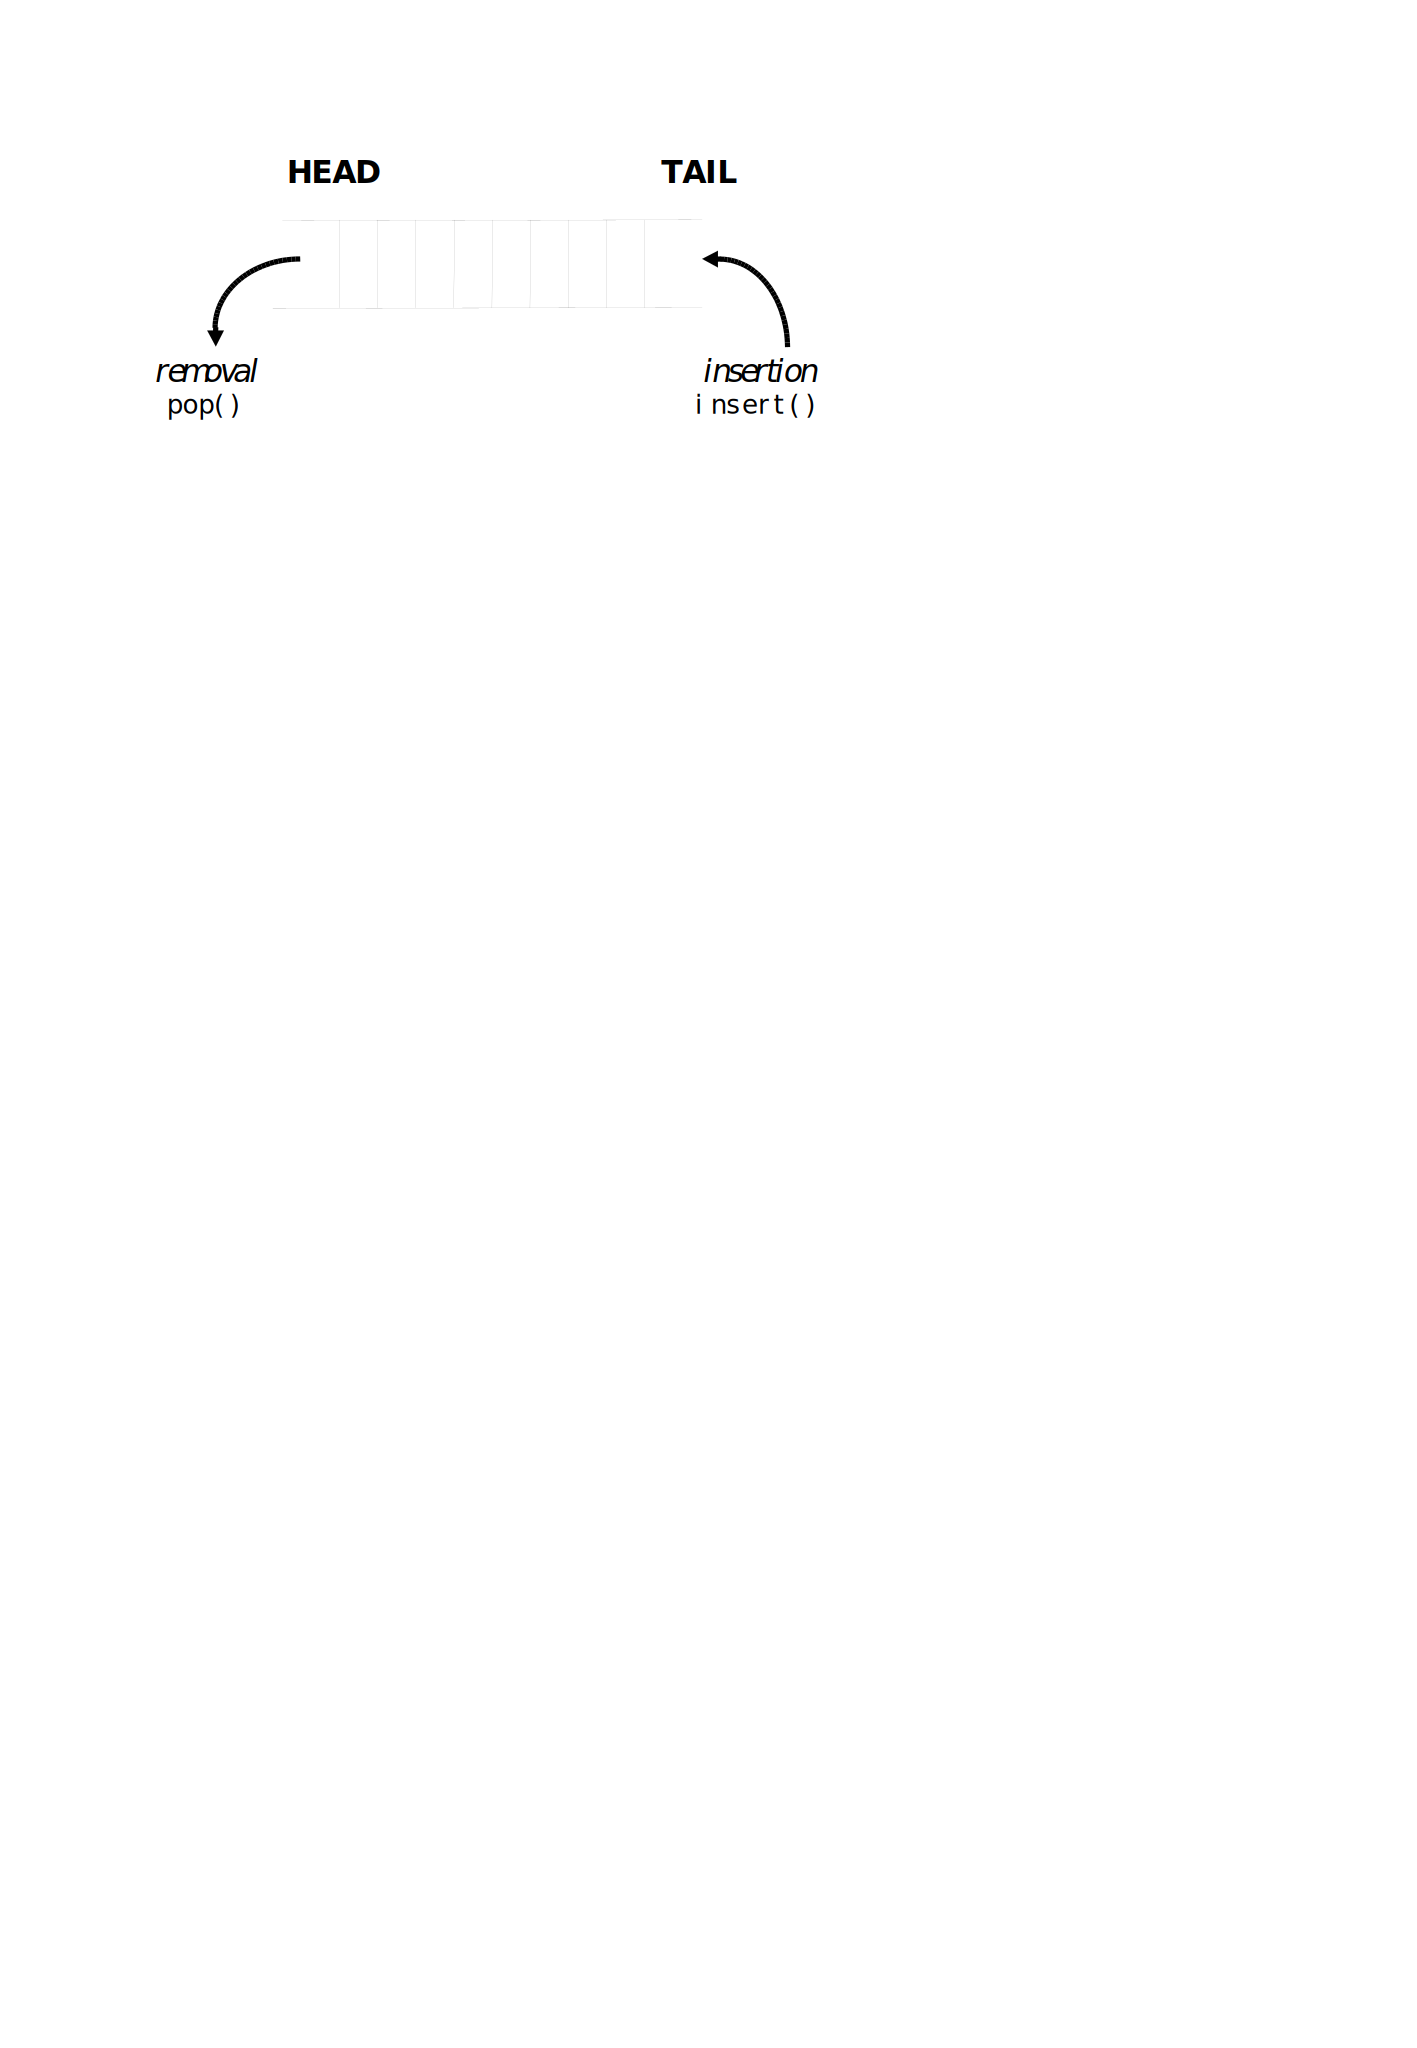
\includegraphics[width=3.703in, height=1.303in]{figures/usmanFig10}
    \caption{cQueue: insertion and removal}
    \label{fig:ch-sim-lib:cqueue}
  \end{center}
\end{figure}

The basic \cclass{cQueue} member functions dealing with insertion and removal
are \fname{insert()} and \fname{pop()}. They are used
like this:

\begin{verbatim}
cQueue queue("my-queue");
cMessage *msg;

// insert messages
for (int i=0; i<10; i++)
{
  msg = new cMessage;
  queue.insert( msg );
}

// remove messages
while( ! queue.empty() )
{
  msg = (cMessage *)queue.pop();
  delete msg;
}
\end{verbatim}


The \fname{length()} member function returns the number of items in the
queue, and \fname{empty()} tells whether there's anything in the queue.

There are other functions dealing with insertion and removal.  The
\fname{insertBefore()} and \fname{insertAfter()} functions insert a
new item exactly before and after a specified one, regardless of the
ordering function.

The \fname{tail()} and \fname{head()} functions return pointers to the objects
at the tail and head of the queue, without affecting queue contents.

The \fname{pop()} function can be used to remove items from the
tail of the queue, and the \fname{remove()} function can be
used to remove any item known by its pointer from the queue:

\begin{verbatim}
queue.remove( msg );
\end{verbatim}



\subsubsection{Priority queue}


By default, \cclass{cQueue} implements a FIFO, but it can also act as
a priority queue, that is, it can keep the inserted objects
ordered\index{queue!order}.  If you want to use this feature, you have
to provide a function that takes two \cclass{cOwnedObject} pointers,
compares the two objects and returns -1, 0 or 1 as the result (see the
reference for details).  An example of setting up an ordered
\cclass{cQueue}:

\begin{verbatim}
cQueue sortedqueue("sortedqueue", cOwnedObject::cmpbyname, true );
                        // sorted by object name, ascending
\end{verbatim}


If the queue object is set up as an ordered queue, the \fname{insert()}
function uses the ordering function: it searches the queue contents
from the head until it reaches the position where the new item
needs to be inserted, and inserts it there.


\subsubsection{Iterators}


Normally, you can only access the objects at the head or tail of the
queue. However, if you use an iterator class, \cclass{cQueue::Iterator},
you can examine each object in the queue\index{queue!iteration}.

The \cclass{cQueue::Iterator} constructor takes two arguments, the first
is the queue object and the second one specifies the initial position
of the iterator: 0=tail, 1=head. Otherwise it acts as any other
{\opp} iterator class: you can use the ++ and -- operators to advance
it, the () operator to get a pointer to the current item, and the
\fname{end()} member function to examine if you're at the end (or the
beginning) of the queue.


An example:

\begin{verbatim}
for( cQueue::Iterator iter(queue,1); !iter.end(), iter++)
{
  cMessage *msg = (cMessage *) iter();
  //...
}
\end{verbatim}




\subsection{Expandable array: cArray}

\subsubsection{Basic usage}


\cclass{cArray} is a container class that holds objects derived from
\cclass{cOwnedObject}. \cclass{cArray} stores the pointers of the objects
inserted instead of making copies. \cclass{cArray} works as an array,
but it grows automatically when it gets full. Internally,
\cclass{cArray} is implemented with an array of pointers; when the array
fills up, it is reallocated.

\cclass{cArray} objects are used in {\opp} to store parameters
attached to messages, and internally, for storing module parameters
and gates.


Creating an array:

\begin{verbatim}
cArray array("array");
\end{verbatim}

Adding an object at the first free index:

\begin{verbatim}
cPar *p = new cPar("par");
int index = array.add( p );
\end{verbatim}


Adding an object at a given index (if the index is occupied,
you'll get an error message):

\begin{verbatim}
cPar *p = new cPar("par");
int index = array.addAt(5,p);
\end{verbatim}


Finding an object in the array:

\begin{verbatim}
int index = array.find(p);
\end{verbatim}

Getting a pointer to an object at a given index:

\begin{verbatim}
cPar *p = (cPar *) array[index];
\end{verbatim}

You can also search the array or get a pointer to an object by
the object's name:

\begin{verbatim}
int index = array.find("par");
Par *p = (cPar *) array["par"];
\end{verbatim}


You can remove an object from the array by calling \fname{remove()}
with the object name, the index position or the object pointer:

\begin{verbatim}
array.remove("par");
array.remove(index);
array.remove( p );
\end{verbatim}


The \fname{remove()} function doesn't deallocate the object, but it
returns the object pointer. If you also want to deallocate it, you can
write:

\begin{verbatim}
delete array.remove( index );
\end{verbatim}

\subsubsection{Iteration}


\cclass{cArray} has no iterator, but it is easy to loop through all the
indices with an integer variable. The \fname{items()} member function
returns the largest index plus one.

\begin{verbatim}
for (int i=0; i<array.items(); i++)
{
  if (array[i]) // is this position used?
  {
    cOwnedObject *obj = array[i];
    ev << obj->name() << endl;
  }
}
\end{verbatim}


%
% \section{Non-object container classes}
%
% There are two container classes to store non-object
% items\index{non-object container}: \cclass{cLinkedList} and
% \cclass{cBag}.  The first one parallels with \cclass{cQueue}, the
% second one with \cclass{cArray}. They can be useful if you have to
% deal with C structs or objects that are not derived from
% \cclass{cOwnedObject}.
%
% See the class library reference for more info about them.
%




\section{The parameter class: cPar}
\label{sec:ch-sim-lib:cpar}

Module parameters (as discussed in section \ref{ch:simple-modules:parameters})
are represented as \cclass{cPar} objects.
The module parameter name is the \cclass{cPar} object's name, and the object
can store any parameter type supported by the NED language, that is,
numeric (long or double), bool, string and XML config file reference.
    \footnote{\cclass{cPar} objects used to be employed also for adding
    parameters (extra fields) to \cclass{cMessage}. While technically this is
    still feasible, message definitions (section \ref{ch:messages:message-definitions})
    are a far superior solution in every respect.}

Module parameters are accessed via \cclass{cModule}'s \fname{par()} method:

\begin{verbatim}
cPar& par(const char *parameterName);
\end{verbatim}

\subsection{Reading the value}

\cclass{cPar} has a number of methods for getting the parameter's value:

\begin{verbatim}
bool boolValue();
long longValue();
const char *stringValue();
double doubleValue();
cXMLElement *xmlValue();
\end{verbatim}

There are also overloaded type cast operators for C/C++ primitive types
including \ttt{bool}, \ttt{int}, \ttt{long}, \ttt{double}, \ttt{const char *},
and also for \ttt{cXMLElement *}.
    \footnote{\cclass{cPar} also supports the \ttt{void *} and \ttt{cOwnedObject *} types,
    but these types were used primarily for message parameters before
    message definitions (section \ref{ch:messages:message-definitions})
    got supported, and you cannot create such module parameters from NED.}

Thus, any of the following ways would work to store a parameter's value in
a variable:

\begin{verbatim}
double foo = par("foo").doubleValue();
double foo = (double) par("foo");
double foo = par("foo");
\end{verbatim}

If you use the \ttt{par("foo")} parameter in expressions (such as
\ttt{4*par("foo")+2}), the C++ compiler may be unable to decide
between overloaded operators and report ambiguity. In that case
you have to clarify by adding either an explicit cast
(\ttt{(double)par("foo")} or \ttt{(long)par("foo")}) or use
the \ttt{doubleValue()} or \ttt{longValue()} methods.

The \fname{isConstant()} method can be used to determine whether a
\cclass{cPar} stores a constant, or an expression that may produce a different
value every time the object is read, such as \ttt{1+exponential(0.5)}.


\subsection{Changing the value}

There are many ways to set a \cclass{cPar}'s value. One is the \ttt{set...Value()}
member functions:

\begin{verbatim}
cPar& foo = par("foo");
foo.setLongValue(12);
foo.setDoubleValue(2.7371);
foo.setStringValue("one two three");
\end{verbatim}

There are also overloaded assignment operators for C++ primitive types,
\ttt{const char *}, and \ttt{cXMLElement *}.

\begin{verbatim}
cPar pp("pp");
pp = 12;
pp = 2.7371;
pp = "one two three";
\end{verbatim}

The \cclass{cPar} object makes its own copy of the string, so the
original one does not need to be preserved. Short strings (less than
\ensuremath{\sim}20 chars) are handled more efficiently because they
are stored in the object's memory space (and are not dynamically
allocated).

\cclass{cPar} can also store other types which yield numeric
results such as function with constant args;
they will be mentioned in the next section.

For numeric and string types, an input flag\index{input flag} can be
set. In this case, when the object's value is first used, the
parameter value will be searched for in the configuration (ini)
file\index{ini file}; if it is not found there, the user will be offered
to enter the value interactively.

Examples:

\begin{verbatim}
cPar foo("foo");
foo.setPrompt("Enter foo value:");
foo.setInput(true);   // make it an input parameter

double d = (double)foo; // the user will be prompted HERE
\end{verbatim}

Further \ttt{set..()} functions to assign other storage types,
e.g. double function with constant args (MathFuncNoArgs, MathFunc1Args, etc),
reverse Polish expression, compiled expressions based on
\cclass{cDoubleExpression}, random distribution based on a
\cclass{cStatistic}'s \fname{random()} method, pointer to \cclass{cOwnedObject},
etc. are listed in the next section; however, they are rarely useful
for programming simulation models.


%
% \subsection{Storing object and non-object pointers in cPar}
% \subsection{Reverse Polish expressions}
% \subsection{Using redirection}
%
% These section got dumped in 3.0, they can be digged out from the CVS if needed.
%

\subsection{cPar storage types}

\cclass{cPar} supports the basic data types (long, double, bool, string, XML) via
several \textit{storage types}. Storage types are internally
identified by type characters. The type character is
returned by the \fname{type()} method.

Example:

\begin{verbatim}
cPar par = 10L;
char typechar = par.type(); // returns storage type 'L'
\end{verbatim}

The all \cclass{cPar} data types and are summarized in the table below.
The \fname{isNumeric()} function tells whether the object
stores a data types which allows the \fname{doubleValue()} method
to be called.

\begin{longtable}{|p{0.7cm}|p{1.2cm}|p{5.2cm}|p{6cm}|}
\hline
% ROW 1
\tabheadcol
\textbf{Type\linebreak char} &
\textbf{Storage\linebreak type} &
\textbf{Member functions} &
\textbf{Description}\\
\hline
%% ROW 2
S &  string &
\ttt{setStringValue( \linebreak
\hspace*{0.3cm}  const char *); \linebreak
const char * \linebreak
\hspace*{0.3cm} \fname{stringValue()}; \linebreak
op const char *(); \linebreak
op=(const char *);} &
{\raggedright
string value. Short strings (len\texttt{<}=27) are stored inside
\cclass{cPar} object, without using heap allocation.}\\\hline
%% ROW 3
B &  boolean &
\ttt{setBoolValue(bool); \linebreak
bool \fname{boolValue()}; \linebreak
op \fname{bool()}; \linebreak
op=(bool);} &
boolean value. Can also be retrieved from the object as long  (0 or 1).\\\hline
%% ROW 4
L & long int &
\ttt{setLongValue(long); \linebreak
long \fname{longValue()}; \linebreak
op \fname{long()}; \linebreak
op=(long);} &
signed long integer value. Can also be retrieved from the object
as double.\\\hline
%% ROW 5
D & double &
\ttt{setDoubleValue(double); \linebreak
double \fname{doubleValue()}; \linebreak
op \fname{double()}; \linebreak
op=(double);} &
double-precision floating point value.\\\hline
%% ROW 6
F & function &
\ttt{setDoubleValue( \linebreak
\hspace*{0.3cm} MathFunc, \linebreak
\hspace*{0.3cm} [double], \linebreak
\hspace*{0.3cm} [double], \linebreak
\hspace*{0.3cm} [double]); \linebreak
double \fname{doubleValue()}; \linebreak
op \fname{double()}; \linebreak
} &
Mathematical function with constant arguments. The function
is given by its pointer; it must take 0,1,2 or 3 doubles and
return a double. This type is mainly used to generate random
numbers: e.g. the function takes mean and standard deviation
and returns a random variable of a certain distribution.\\\hline
%% ROW 7
X & expr. &
\ttt{setDoubleValue( \linebreak
\hspace*{0.3cm} cPar::ExprElem*,int); \linebreak
double \fname{doubleValue()}; \linebreak
op \fname{double()};}
&
Runtime-evaluated Reverse Polish expression. Expression can contain constants,
\cclass{cPar} objects, refer to other \cclass{cPars} (e.g. module parameters),
can use math operators (+-*/{\textasciicircum}\% etc), function calls
(function must take 0,1,2 or 3 doubles and return a double).
The expression must be given in an array of \ttt{cPar::ExprElem} structs.\\\hline
%% ROW 7a
C & compiled\linebreak expr. &
\ttt{setDoubleValue( \linebreak
\hspace*{0.3cm} cDoubleExpression *expr); \linebreak
double \fname{doubleValue()}; \linebreak
op \fname{double()};}
&
Runtime-evaluated compiled expression. The expression should be
supplied in a method of an object subclassed from \cclass{cDoubleExpression}.
\\\hline
%% ROW 8
T & distrib. &
\ttt{setDoubleValue( \linebreak
\hspace*{0.3cm} \cclass{cStatistic}*); \linebreak
double \fname{doubleValue()}; \linebreak
op \fname{double()}; \linebreak
} &
random variable generated from a distribution collected by a
statistical data collection object (derived from \cclass{cStatistic}).\\\hline
%% ROW 8a
M & XML &
\ttt{setXMLValue( \linebreak
\hspace*{0.3cm} \cclass{cXMLElement} *node); \linebreak
\cclass{cXMLElement} *\fname{xmlValue}()}; \linebreak
op \fname{cXMLElement*()};
&
Reference to an XML element, found in an XML config file.
\\\hline
%% ROW 9
P & void* pointer &
\ttt{setPointerValue(void*); \linebreak
void *\fname{pointerValue()}; \linebreak
op void *(); \linebreak
op=(void *);} &
pointer to a non-\cclass{cOwnedObject} item (C struct, non-\cclass{cOwnedObject} object
etc.) Memory management can be controlled through the \fname{configPointer()}
member function.\\\hline
%% ROW 10
O & object pointer &
\ttt{setObjectValue(cOwnedObject*); \linebreak
cOwnedObject *\fname{objectValue()}; \linebreak
op cOwnedObject *(); \linebreak
op=(cOwnedObject *);}
&
{\raggedright pointer to an object derived from \cclass{cOwnedObject}.
Ownership management is done through \fname{takeOwnership()}.}\\\hline
%% ROW 11
I & indirect value &
\ttt{setRedirection(cPar*); \linebreak
bool \fname{isRedirected()}; \linebreak
cPar *\fname{redirection()}; \linebreak
\fname{cancelRedirection()};}
&
{\raggedright value is redirected to another \cclass{cPar} object. All value setting
and reading operates on the other \cclass{cPar}; even the \fname{type()} function
will return the type in the other \cclass{cPar} (so you'll never get 'I'
as the type). This redirection can only be broken with the \fname{cancelRedirection()}
member function. Module parameters taken by \ttt{ref} use this mechanism.}\\\hline
\end{longtable}


%FIXME document: cXMLElement
%FIXME document: simulation.getUniqueNumber(), for generating unique IDs for models


\section{Routing support: cTopology}

\subsection{Overview}

The \cclass{cTopology} class was designed primarily to support
routing\index{routing support} in telecommunication or multiprocessor
networks.

A \cclass{cTopology} object stores an abstract representation of the
network in graph form:
\begin{itemize}
  \item{each \cclass{cTopology} node corresponds to a \textit{module}
    (simple or compound), and}
  \item{each \cclass{cTopology} edge corresponds to a \textit{link} or
    \textit{series of connecting links}.}
\end{itemize}

You can specify which modules (either simple or compound) you want to
include in the graph. The graph will include all connections among the
selected modules. In the graph, all nodes are at the same level,
there's no submodule nesting.  Connections which span across compound
module boundaries are also represented as one graph edge. Graph edges
are directed, just as module gates are.


If you're writing a router or switch model, the \cclass{cTopology}
graph can help you determine what nodes are available through which
gate and also to find optimal routes\index{optimal routes}. The
\cclass{cTopology} object can calculate shortest paths\index{shortest
  path} between nodes for you.

The mapping between the graph (nodes, edges) and network model
(modules, gates, connections) is preserved: you can easily find
the corresponding module for a \cclass{cTopology} node and vica versa.





\subsection{Basic usage}

You can extract the network topology into a \cclass{cTopology}
object by a single function call. You have several ways to select
which modules you want to include in the topology:
\begin{itemize}
  \item{by module type}
  \item{by a parameter's presence and its value}
  \item{with a user-supplied boolean function}
\end{itemize}

First, you can specify which node types you want to include. The
following code extracts all modules of type \ttt{Router} or \ttt{Host}.
(\ttt{Router} and \ttt{Host} can be either simple or compound module types.)

\begin{verbatim}
cTopology topo;
topo.extractByModuleType("Router", "Host", NULL);
\end{verbatim}

Any number of module types can be supplied; the list must be terminated by \ttt{NULL}.

A dynamically assembled list of module types can be passed as a
\ttt{NULL}-terminated array of \ttt{const char*} pointers, or
in an STL string vector \ttt{std::vector<std::string>}.
An example for the former:

\begin{verbatim}
cTopology topo;
const char *typeNames[3];
typeNames[0] = "Router";
typeNames[1] = "Host";
typeNames[2] = NULL;
topo.extractByModuleType(typeNames);
\end{verbatim}

Second, you can extract all modules which have a certain parameter:

\begin{verbatim}
topo.extractByParameter( "ipAddress" );
\end{verbatim}

You can also specify that the parameter must have a certain value
for the module to be included in the graph:

\begin{verbatim}
cPar yes = "yes";
topo.extractByParameter( "includeInTopo", &yes );
\end{verbatim}

The third form allows you to pass a function which can determine for
each module whether it should or should not be included.  You can have
\cclass{cTopology} pass supplemental data to the function through a
\ttt{void*} pointer. An example which selects all top-level modules (and
does not use the \ttt{void*} pointer):

\begin{verbatim}
int selectFunction(cModule *mod, void *)
{
  return mod->parentModule() == simulation.systemModule();
}

topo.extractFromNetwork( selectFunction, NULL );
\end{verbatim}

%
% TBD one more example which \textit{does use} the void* ptr.
%

A \cclass{cTopology} object uses two types: \cclass{cTopology::Node} for
nodes and \cclass{cTopology::Link} for edges. (\cclass{sTopo\-Link\-In} and
\cclass{cTopology::LinkOut} are `aliases' for \cclass{cTopology::Link}; we'll
talk about them later.)

Once you have the topology extracted, you can start exploring
it. Consider the following code (we'll explain it shortly):

\begin{verbatim}
for (int i=0; i<topo.nodes(); i++)
{
  cTopology::Node *node = topo.node(i);
  ev << "Node i=" << i << " is " << node->module()->fullPath() << endl;
  ev << " It has " << node->outLinks() << " conns to other nodes\n";
  ev << " and " << node->inLinks() << " conns from other nodes\n";

  ev << " Connections to other modules are:\n";
  for (int j=0; j<node->outLinks(); j++)
  {
    cTopology::Node *neighbour = node->out(j)->remoteNode();
    cGate *gate = node->out(j)->localGate();
    ev << " " << neighbour->module()->fullPath()
       << " through gate " << gate->fullName() << endl;
  }
}
\end{verbatim}

The \fname{nodes()} member function (1st line) returns the number of
nodes in the graph, and node(i) returns a pointer to the \textit{i}th
node, an \cclass{cTopology::Node} structure.


The correspondence between a graph node and a module can be obtained
by:

\begin{verbatim}
cTopology::Node *node = topo.nodeFor( module );
cModule *module = node->module();
\end{verbatim}


The \fname{nodeFor()} member function returns a pointer to the graph
node for a given module. (If the module is not in the graph, it
returns \ttt{NULL}). \fname{nodeFor()} uses binary search within the
\cclass{cTopology} object so it is fast enough.


\cclass{cTopology::Node}'s other member functions let you determine the
connections of this node: \fname{inLinks()}, \fname{outLinks()} return
the number of connections, \ttt{in(i)} and
\ttt{out(i)} return pointers to graph edge objects.


By calling member functions of the graph edge object, you can
determine the modules and gates involved. The \fname{remoteNode()}
function returns the other end of the connection, and
\fname{localGate()}, \fname{remoteGate()}, \fname{localGateId()} and
\fname{remoteGateId()} return the gate pointers and ids of the gates
involved. (Actually, the implementation is a bit tricky here: the same
graph edge object \cclass{cTopology::Link} is returned either as
\cclass{cTopology::LinkIn} or as \cclass{cTopology::LinkOut} so that ``remote''
and ``local'' can be correctly interpreted for edges of both
directions.)





\subsection{Shortest paths}

The real power of \cclass{cTopology} is in finding shortest
paths\index{topology!shortest path} in the network to support optimal
routing\index{optimal routing}. \cclass{cTopology} finds shortest paths
from \textit{all} nodes \textit{to} a target node. The algorithm is
computationally inexpensive. In the simplest case, all edges are
assumed to have the same weight.

A real-life example when we have the target module pointer, finding
the shortest path looks like this:

\begin{verbatim}
cModule *targetmodulep =...;
cTopology::Node *targetnode = topo.nodeFor( targetmodulep );
topo.unweightedSingleShortestPathsTo( targetnode );
\end{verbatim}


This performs the Dijkstra algorithm\index{Dijkstra algorithm} and
stores the result in the \cclass{cTopology} object. The result can
then be extracted using \cclass{cTopology} and
\ttt{cTopology::Node}\index{cTopology::Node} methods.  Naturally, each call to
\fname{unweightedSingleShortestPathsTo()} overwrites the results of
the previous call.

Walking along the path from our module to the target node:

\begin{verbatim}
cTopology::Node *node = topo.nodeFor( this );

if (node == NULL)
{
  ev < "We (" << fullPath() << ") are not included in the topology.\n";
}
else if (node->paths()==0)
{
  ev << "No path to destination.\n";
}
else
{
  while (node != topo.targetNode())
  {
    ev << "We are in " << node->module()->fullPath() << endl;
    ev << node->distanceToTarget() << " hops to go\n";
    ev << "There are " << node->paths()
       << " equally good directions, taking the first one\n";
    cTopology::LinkOut *path = node->path(0);
    ev << "Taking gate " << path->localGate()->fullName()
       << " we arrive in " << path->remoteNode()->module()->fullPath()
       << " on its gate " << path->remoteGate()->fullName() << endl;
    node = path->remoteNode();
  }
}
\end{verbatim}


The purpose of the \fname{distanceToTarget()} member function of a
node is self-explanatory. In the unweighted case, it returns the
number of hops. The \fname{paths()} member function returns the number
of edges which are part of a shortest path, and
\fname[path()]{path(i)} returns the \textit{i}th edge of them as
\cclass{cTopology::LinkOut}. If the shortest paths were created by the
\fname[SingleShortestPaths()]{...SingleShortestPaths()} function,
\fname{paths()} will always return 1 (or 0 if the target is not
reachable), that is, only one of the several possible shortest paths
are found.  The
\fname[MultiShortestPathsTo()]{...MultiShortestPathsTo()} functions
find all paths, at increased run-time cost. The \cclass{cTopology}'s
\fname{targetNode()} function returns the target node of the last
shortest path search.

You can enable/disable nodes or edges in the graph. This is done by
calling their \fname{enable()} or \fname{disable()} member functions.
Disabled nodes or edges are ignored by the shortest paths calculation
algorithm. The \fname{enabled()} member function returns the state of
a node or edge in the topology graph.

One usage of \fname{disable()} is when you want to determine in how many
hops the target node can be reached from our node \textit{through
a particular output gate}. To calculate this, you calculate the
shortest paths to the target \textit{from the neighbor node}, but
you must disable the current node to prevent the shortest paths
from going through it:

\begin{verbatim}
cTopology::Node *thisnode = topo.nodeFor( this );
thisnode->disable();
topo.unweightedSingleShortestPathsTo( targetnode );
thisnode->enable();

for (int j=0; j<thisnode->outLinks(); j++)
{
  cTopology::LinkOut *link = thisnode->out(i);
  ev << "Through gate " << link->localGate()->fullName() << " : "
     << 1 + link->remoteNode()->distanceToTarget() << " hops" << endl;
}
\end{verbatim}

In the future, other shortest path algorithms will also be implemented:

\begin{verbatim}
unweightedMultiShortestPathsTo(cTopology::Node *target);
weightedSingleShortestPathsTo(cTopology::Node *target);
weightedMultiShortestPathsTo(cTopology::Node *target);
\end{verbatim}






\section{Statistics and distribution estimation}

\subsection{cStatistic and descendants}

There are several statistic and result collection classes:
\cclass{cStdDev}, \cclass{cWeightedStdDev}, \cclass{Long\-Histogram},
\cclass{cDoubleHistogram}, \cclass{cVarHistogram}, \cclass{cPSquare} and
\cclass{cKSplit}. They are all derived from the abstract base class
\cclass{cStatistic}.

\begin{itemize}
  \item{\cclass{cStdDev} keeps number of samples, mean, standard
    deviation, minimum and maximum value etc.}
  \item{\cclass{cWeightedStdDev} is similar to \cclass{cStdDev}, but
    accepts weighted observations. \cclass{cWeightedStdDev} can be used
    for example to calculate time average. It is the only weighted
    statistics class.}
  \item{\cclass{cLongHistogram} and \cclass{cDoubleHistogram} are
    descendants of \cclass{cStdDev} and also keep an approximation of
    the distribution of the observations using equidistant
    (equal-sized) cell histograms\index{histogram!equal-sized}.}
  \item{\cclass{cVarHistogram} implements a histogram where cells do not
    need to be the same size. You can manually add the cell (bin)
    boundaries, or alternatively, automatically have a partitioning
    created where each bin has the same number of observations (or as
    close to that as possible).}
  \item{\cclass{cPSquare} is a class that uses the $P^{2}$ algorithm
    described in \cite{JCh85}. The algorithm calculates quantiles without
    storing the observations; one can also think of it as a histogram
    with equiprobable cells\index{histogram!equiprobable-cells}.}
  \item{\cclass{cKSplit} uses a novel, experimental method, based on an
    adaptive histogram-like algorithm.}
\end{itemize}

\subsubsection{Basic usage}

One can insert an observation into a statistic object with the
\fname{collect()} function or the \texttt{+=} operator (they are
equivalent).  \cclass{cStdDev} has the following methods for getting
statistics out of the object: \fname{samples()}, \fname{min()},
\fname{max()}, \fname{mean()}, \fname{stddev()}, \fname{variance()},
\fname{sum()}, \fname{sqrSum()} with the obvious meanings. An example
usage for \cclass{cStdDev}:

\begin{verbatim}
cStdDev stat("stat");

for (int i=0; i<10; i++)
  stat.collect( normal(0,1) );

long numSamples = stat.samples();
double smallest = stat.min(),
       largest = stat.max();
double mean = stat.mean(),
       standardDeviation = stat.stddev(),
       variance = stat.variance();
\end{verbatim}





\subsection{Distribution estimation}

\subsubsection{Initialization and usage}

% TBD this has to be rewritten at some point... maybe take over examples from Doxygen doc.

The distribution estimation\index{distribution!estimation} classes
(\cclass{cLongHistogram}, \cclass{cDoubleHistogram}, \cclass{cVarHistogram},
\cclass{cPSquare} and \cclass{cKSplit}) are derived from
\cclass{cDensityEstBase}. Distribution estimation classes (except for
\cclass{cPSquare}) assume that the observations are within a range.
You may specify the range explicitly (based on some a-priori info
about the distribution) or you may let the object collect the first
few observations and determine the range from them. Methods which let
you specify range settings are part of \cclass{cDensityEstBase}.

The following member functions exist for setting up the range
and to specify how many observations should be used for
automatically determining the range.

\begin{verbatim}
setRange(lower,upper);
setRangeAuto(numFirstvals, rangeExtFactor);
setRangeAutoLower(upper, numFirstvals, rangeExtFactor);
setRangeAutoUpper(lower, numFirstvals, rangeExtFactor);
\end{verbatim}

\begin{verbatim}
setNumFirstVals(numFirstvals);
\end{verbatim}

The following example creates a histogram with 20 cells and automatic
range estimation\index{histogram!range estimation}:

\begin{verbatim}
cDoubleHistogram histogram("histogram", 20);
histogram.setRangeAuto(100,1.5);
\end{verbatim}


Here, 20 is the number of cells (not including the underflow/overflow
cells, see later), and 100 is the number of observations to be
collected before setting up the cells. 1.5 is the range extension
factor. It means that the actual range of the initial observations
will be expanded 1.5 times and this expanded range will be used to lay
out the cells. This method increases the chance that further
observations fall in one of the cells and not outside the histogram
range.

\begin{figure}[htbp]
  \begin{center}
    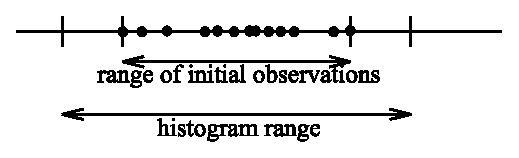
\includegraphics[width=3.215in, height=0.930in]{figures/usmanFig12}
    \caption{Setting up a histogram's range}
  \end{center}
\end{figure}

After the cells have been set up, collection can go on.

The \fname{transformed()} function returns \textit{true} when the cells have
already been set up. You can force range estimation and setting
up the cells by calling the \fname{transform()} function.

The observations that fall outside the histogram range will be counted
as underflows and overflows. The number of underflows and overflows
are returned by the \fname{underflowCell()} and \fname{overflowCell()}
member functions.

\begin{figure}[htbp]
\begin{center}
  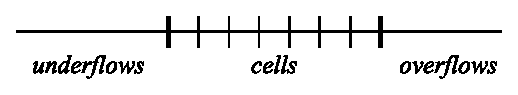
\includegraphics[width=3.310in, height=0.467in]{figures/usmanFig13}
  \caption{Histogram structure after setting up the cells}
\end{center}
\end{figure}

You create a $P^{2}$ object by specifying the number of cells:

\begin{verbatim}
cPSquare psquare("interarrival-times", 20);
\end{verbatim}

Afterwards, a \cclass{cPSquare} can be used with the same member functions
as a histogram.


\subsubsection{Getting histogram data}


There are three member functions to explicitly return cell boundaries
and the number of observations is each cell. \fname{cells()} returns
the number of cells, \fname[basepoint()]{basepoint(int k)} returns the
\textit{k}th base point, \fname[cell()]{cell(int k)} returns the
number of observations in cell \textit{k}, and
\fname[cellPDF()]{cellPDF(int k)} returns the PDF value in the cell
(i.e. between \fname[basepoint()]{basepoint(k)} and
\fname[basepoint()]{basepoint(k+1)}).  These functions work for all
histogram types, plus \cclass{cPSquare} and \cclass{cKSplit}.

\begin{figure}[htbp]
  \begin{center}
    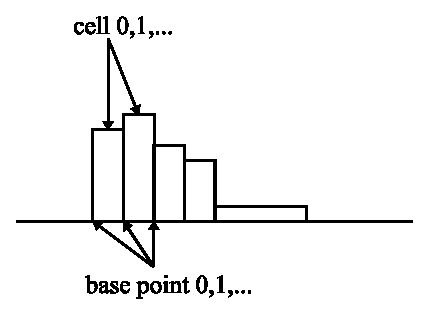
\includegraphics[width=2.615in, height=2.001in]{figures/usmanFig14}
    \caption{base points and cells}
  \end{center}
\end{figure}

An example:

\begin{verbatim}
long n = histogram.samples();
for (int i=0; i<histogram.cells(); i++)
{
  double cellWidth = histogram.basepoint(i+1)-histogram.basepoint(i);
  int count = histogram.cell(i);
  double pdf = histogram.cellPDF(i);
  //...
}
\end{verbatim}


The \fname[pdf()]{pdf(x)} and \fname[cdf()]{cdf(x)} member functions
return the value of the Probability Density Function and the Cumulated
Density Function at a given \textit{x}, respectively.


\subsubsection{Random number generation from distributions}


The \fname{random()} member function generates random
numbers\index{random!numbers} from the distribution stored by the
object:

\begin{verbatim}
double rnd = histogram.random();
\end{verbatim}


\cclass{cStdDev} assumes normal distribution.

You can also wrap the distribution object in a \cclass{cPar}:

\begin{verbatim}
cPar rndPar("rndPar");
rndPar.setDoubleValue(&histogram);
\end{verbatim}


The \cclass{cPar} object stores the pointer to the histogram (or $P^{2}$ object),
and whenever it is asked for the value, calls the histogram object's \fname{random()}
function:

\begin{verbatim}
double rnd = (double)rndPar; // random number from the cPSquare
\end{verbatim}

\subsubsection{Storing/loading distributions}


The statistic classes have \fname{loadFromFile()} member functions
that read the histogram data from a text file. If you need a custom
distribution\index{distribution!custom} that cannot be written (or it
is inefficient) as a C function, you can describe it in histogram form
stored in a text file, and use a histogram object with
\fname{loadFromFile()}.

You can also use \fname{saveToFile()}that writes out the distribution
collected by the histogram object:

\begin{verbatim}
FILE *f = fopen("histogram.dat","w");
histogram.saveToFile(f); // save the distribution
fclose(f);

cDoubleHistogram hist2("Hist-from-file");
FILE *f2 = fopen("histogram.dat","r");
hist2.loadFromFile(f2); // load stored distribution
fclose(f2);
\end{verbatim}


\subsubsection{Histogram with custom cells}


The \cclass{cVarHistogram} class can be used to create
histograms with arbitrary (non-equidistant) cells.
It can operate in two modes:

\begin{itemize}
  \item \textit{manual}, where you specify cell boundaries explicitly
     before starting collecting
  \item \textit{automatic}, where \fname{transform()} will set up the cells
     after collecting a certain number of initial observations. The cells
     will be set up so that as far as possible, an equal number of observations
     fall into each cell (equi-probable cells).
\end{itemize}

Modes are selected with a \textit{transform-type} parameter:
\begin{itemize}
  \item{\ttt{HIST\_TR\_NO\_TRANSFORM}: no transformation; uses bin boundaries
    previously defined by \fname{addBinBound()}}
  \item{\ttt{HIST\_TR\_AUTO\_EPC\_DBL}: automatically creates equiprobable cells}
  \item{\ttt{HIST\_TR\_AUTO\_EPC\_INT}: like the above, but for integers}
\end{itemize}

Creating an object:

\begin{verbatim}
cVarHistogram(const char *s=NULL,
              int numcells=11,
              int transformtype=HIST_TR_AUTO_EPC_DBL);
\end{verbatim}

Manually adding a cell boundary:

\begin{verbatim}
void addBinBound(double x);
\end{verbatim}

Rangemin and rangemax is chosen after collecting the
\texttt{numFirstVals} initial observations. One cannot add cell
boundaries when the histogram has already been transformed.





\subsection{The k-split algorithm}

\subsubsection{Purpose}


The \textit{k}-split algorithm is an on-line distribution
estimation\index{distribution!online estimation} method.  It was
designed for on-line result collection in simulation programs.  The
method was proposed by Varga and Fakhamzadeh in 1997. The primary
advantage of \textit{k}-split is that without having to store the
observations, it gives a good estimate without requiring a-priori
information about the distribution, including the sample size. The
\textit{k}-split algorithm can be extended to multi-dimensional
distributions\index{distribution!multi-dimensional}, but here we deal
with the one-dimensional version only.


\subsubsection{The algorithm}


The \textit{k-split} algorithm is an adaptive histogram-type estimate which
maintains a good partitioning by doing cell splits. We start out with
a histogram range $[x_{lo}, x_{hi})$ with $k$ equal-sized histogram
cells with observation counts $n_1,n_2, \cdots n_k$.  Each collected
observation increments the corresponding observation count. When an
observation count $n_i$ reaches a \textit{split threshold}, the cell
is split into $k$ smaller, equal-sized cells with observation counts
$n_{i,1}, n_{i,2}, \cdots n_{i,k}$ initialized to zero. The $n_i$
observation count is remembered and is called the \textit{mother
  observation count} to the newly created cells. Further observations
may cause cells to be split further (e.g. $n_{i,1,1},...n_{i,1,k}$
etc.), thus creating a $k$-order tree of observation counts where
leaves contain live counters that are actually incremented by new
observations, and intermediate nodes contain mother observation counts
for their children. If an observation falls outside the histogram
range, the range is extended in a natural manner by inserting new
level(s) at the top of the tree. The fundamental parameter to the
algorithm is the split factor $k$. Experience shows that $k=2$ worked best.

\begin{figure}[htbp]
  \begin{center}
    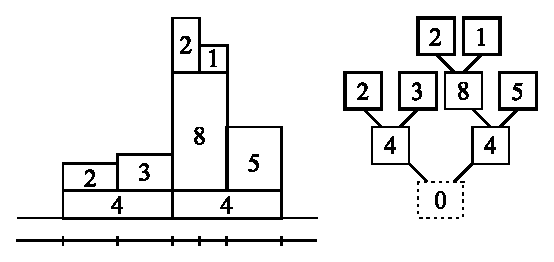
\includegraphics[width=3.442in, height=1.518in]{figures/usmanFig15}
    \caption{Illustration of the k-split algorithm, $k=2$. The
      numbers in boxes represent the observation count values}
  \end{center}
\end{figure}


For density estimation, the total number of observations that
fell into each cell of the partition has to be determined. For
this purpose, mother observations in each internal node of the
tree must be distributed among its child cells and propagated
up to the leaves.

% careful with reformatting! $..$ MUST NOT BE BROKEN TO SEVERAL LINES!

Let $n_{...,i}$ be the (mother) observation count for a cell,
$s_{...,i}$ be the total observation count in a cell $n_{...,i}$ plus
the observation counts in all its sub-, sub-sub-, etc. cells), and
$m_{...,i}$ the mother observations propagated to the cell. We are
interested in the $\tilde{n}_{...,i} = n_{...,i} + m_{...,i}$
estimated amount of observations in the tree nodes, especially in the
leaves. In other words, if we have $\tilde{n}_{...,i}$ estimated
observation amount in a cell, how to divide it to obtain
$m_{...,i,1}, m_{...,i,2} \cdots m_{...,i,k}$
that can be propagated to child cells. Naturally,
$m_{...,i,1} + m_{...,i,2} + \cdots + m_{...,i,k} = \tilde{n}_{...,i}$.

% careful with reformatting! $..$ MUST NOT BE BROKEN TO SEVERAL LINES!

Two natural distribution methods are even
distribution\index{distribution!even} (when
$m_{...,i,1} = m_{...,i,2} = \cdots = m_{...,i,k}$) and proportional
distribution\index{distribution!proportional} (when
$m_{...,i,1} : m_{...,i,2} : \cdots : m_{...,i,k} = s_{...,i,1} : s_{...,i,2} : \cdots : s_{...,i,k}$).
Even distribution is optimal when the
$s_{...,i,j}$ values are very small, and proportional distribution is
good when the $s_{...,i,j}$ values are large compared to
$m_{...,i,j}$. In practice, a linear combination of them seems
appropriate, where $\lambda=0$ means even and $\lambda=1$ means
proportional distribution:

% careful with reformatting! $..$ MUST NOT BE BROKEN TO SEVERAL LINES!

$m_{\cdots,i,j} = (1-\lambda)\tilde{n}_{\cdots,i}/k + \lambda \tilde{n}_{\cdots,i} s_{...,i,j} / s_{\cdots,i}$
where $\lambda\in[0,1]$

\begin{figure}[htbp]
  \begin{center}
    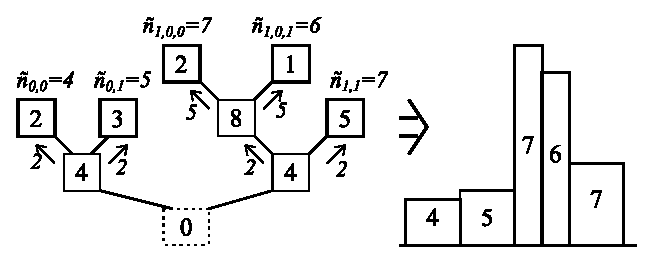
\includegraphics[width=4.147in, height=1.567in]{figures/usmanFig16}
    \caption{Density estimation from the k-split cell tree. We
      assume $\lambda=0$, i.e. we distribute mother observations
      evenly.}
  \end{center}
\end{figure}

% careful with reformatting! $..$ MUST NOT BE BROKEN TO SEVERAL LINES!

Note that while $n_{...,i}$ are integers, $m_{...,i}$ and thus
$\tilde{n}_{...,i}$ are typically real numbers. The histogram estimate
calculated from \textit{k}-split is not exact, because the frequency
counts calculated in the above manner contain a degree of estimation
themselves. This introduces a certain \textit{cell division error};
the $\lambda$ parameter should be selected so that it minimizes that
error. It has been shown that the cell division error can
be reduced to a more-than-acceptable small value.\\
Strictly speaking, the \textit{k}-split algorithm is semi-online,
because its needs some observations to set up the initial histogram
range.  Because of the range extension and cell split
capabilities, the algorithm is not very sensitive to the choice of the
initial range, so very few observations are sufficient for range
estimation (say $N_{pre}=10$). Thus we can regard \textit{k}-split as
an on-line method.

\textit{K}-split can also be used in semi-online mode, when the
algorithm is only used to create an optimal partition from a larger
number of $N_{pre}$ observations. When the partition has been created,
the observation counts are cleared and the $N_{pre}$ observations are
fed into \textit{k}-split once again. This way all mother (non-leaf)
observation counts will be zero and the cell division error is
eliminated. It has been shown that the partition created by
\textit{k}-split can be better than both the equi-distant and the
equal-frequency partition.


{\opp} contains an experimental implementation of the \textit{k}-split
algorithm, the \cclass{cKSplit} class. Research on \textit{k}-split is
still under way.


\subsubsection{The cKSplit class}

The \cclass{cKSplit} class is an implementation of the \textit{k-split} method.
Member functions:

%
% TBD comments
%

\begin{verbatim}
void setCritFunc(KSplitCritFunc _critfunc, double *_critdata);
void setDivFunc(KSplitDivFunc \_divfunc, double *\_divdata);
void rangeExtension( bool enabled );
\end{verbatim}


\begin{verbatim}
int treeDepth();
int treeDepth(sGrid& grid);
\end{verbatim}

\begin{verbatim}
double realCellValue(sGrid& grid, int cell);
void printGrids();
\end{verbatim}

\begin{verbatim}
sGrid& grid(int k);
sGrid& rootGrid();
\end{verbatim}

\begin{verbatim}
struct sGrid
{
  int parent;   // index of parent grid
  int reldepth; // depth = (reldepth - rootgrid's reldepth)
  long total;   // sum of cells & all subgrids (includes `mother')
  int mother;   // observations `inherited' from mother cell
  int cells[K]; // cell values
};
\end{verbatim}



\subsection{Transient detection and result accuracy}

In many simulations, only the steady state performance (i.e.
the performance after the system has reached a stable state)
is of interest. The initial part of the simulation is called
the transient period. After the model has entered steady state,
simulation must proceed until enough statistical data has been
collected to compute result with the required accuracy.


Detection of the end of the transient period and a certain result
accuracy is supported by {\opp}. The user can attach transient
detection\index{transient detection} and result accuracy\index{result
  accuracy} objects to a result object (\cclass{cStatistic}'s
descendants). The transient detection and result accuracy objects will
do the specific algorithms on the data fed into the result object and
tell if the transient period is over or the result accuracy has been
reached.

The base classes for classes implementing specific transient
detection and result accuracy detection algorithms are:
\begin{itemize}
\item{\cclass{cTransientDetection}: base class for transient detection}
\item{\cclass{cAccuracyDetection}: base class for result accuracy detection}
\end{itemize}


\subsubsection{Basic usage}

%
% TBD comments
%

Attaching detection objects to a \cclass{cStatistic} and getting pointers
to the attached objects:

\begin{verbatim}
addTransientDetection(cTransientDetection *object);
addAccuracyDetection(cAccuracyDetection *object);
cTransientDetection *transientDetectionObject();
cAccuracyDetection *accuracyDetectionObject();
\end{verbatim}


Detecting the end of the period:
\begin{itemize}
\item{polling the \fname{detect()} function of the object}
\item{installing a post-detect function}
\end{itemize}


\subsubsection{Transient detection}


Currently one transient detection\index{transient detection} algorithm
is implemented, i.e.  there's one class derived from
\cclass{cTransientDetection}. The \cclass{cTDExpandingWindows} class
uses the sliding window approach with two windows, and checks the
difference of the two averages to see if the transient period is over.

\begin{verbatim}
void setParameters(int reps=3,
                   int minw=4,
                   double wind=1.3,
                   double acc=0.3);
\end{verbatim}

\subsubsection{Accuracy detection}


Currently one accuracy detection\index{accuracy detection} algorithm
is implemented, i.e.  there's one class derived from
\cclass{cAccuracyDetection}. The algorithm implemented in the
\cclass{cADByStddev} class is: divide the standard deviation by the
square of the number of values and check if this is small enough.

\begin{verbatim}
void setParameters(double acc=0.1, int reps=3);
\end{verbatim}




\section{Recording simulation results}

\subsection{Output vectors: cOutVector}
\label{sec:ch-sim-lib:coutvector}

Objects of type \cclass{cOutVector} are responsible for writing time series
data (referred to as \textit{output vectors}) to a file. The \fname{record()}
method is used to output a value (or a value pair) with a timestamp.
The object name will serve as the name of the output vector.

The vector name can be passed in the constructor,

\begin{verbatim}
cOutVector responseTimeVec("response time");
\end{verbatim}

but in the usual arrangement you'd make the \cclass{cOutVector} a member
of the module class and set the name in \fname{initialize()}. You'd
record values from \fname{handleMessage()} or from a function called from
\fname{handleMessage()}.

The following example is a \ttt{Sink} module which records the lifetime
of every message that arrives to it.

\begin{verbatim}
class Sink : public cSimpleModule
{
  protected:
    cOutVector endToEndDelayVec;

    virtual void initialize();
    virtual void handleMessage(cMessage *msg);
};

Define_Module(Sink);

void Sink::initialize()
{
    endToEndDelayVec.setName("End-to-End Delay");
}

void Sink::handleMessage(cMessage *msg)
{
    simtime_t eed = simTime() - msg->creationTime();
    endToEndDelayVec.record(eed);
    delete msg;
}
\end{verbatim}

There is also a \fname{recordWithTimestamp()} method, to make it
possible to record values into output vectors with a timestamp other than
\fname{simTime()}. Increasing timestamp order is still enforced though.

All \cclass{cOutVector} objects write to a single \textit{output vector file}
named \ttt{omnetpp.vec} by default.
You can configure output vectors from \ttt{omnetpp.ini}:
you can disable writing to the file, or limit it to a certain
simulation time interval for recording (section
\ref{sec:ch-run-sim:outvectors}).

The format and processing of output vector files is described in section
\ref{sec:ch-ana-sim:output-vectors}.

If the output vector object is disabled or the simulation time is
outside the specified interval, \fname{record()} doesn't write
anything to the output file. However, if you have a Tkenv inspector
window open for the output vector object\index{output!vector object},
the values will be displayed there, regardless of the state of the
output vector object.



\subsection{Output scalars}

While output vectors are to record time series data and thus they
typically record a large volume of data during a simulation run,
output scalars\index{output!scalars} are supposed to record a single
value per simulation run. You can use output scalars

\begin{itemize}
\item{to record summary data at the end of the simulation run}
\item{to do several runs with different parameter settings/random seed
    and determine the dependence of some measures on the parameter
    settings. For example, multiple runs and output scalars are the
    way to produce \textit{Throughput vs. Offered Load} plots.}
\end{itemize}

Output scalars are recorded with the \fname{recordScalar()} method of
\cclass{cSimpleModule}, and you'll usually want to insert this code
into the \fname{finish()} function. An example:

\begin{verbatim}
void Transmitter::finish()
{
    double avgThroughput = totalBits / simTime();
    recordScalar("Average throughput", avgThroughput);
}
\end{verbatim}

You can record whole statistics objects by calling their \fname{recordScalar()}
methods, declared as part of \cclass{cStatistic}. In the following example
we create a \ttt{Sink} module which calculates the mean, standard
deviation, minimum and maximum values of a variable, and records them at the
end of the simulation.

\begin{verbatim}
class Sink : public cSimpleModule
{
  protected:
    cStdDev eedStats;

    virtual void initialize();
    virtual void handleMessage(cMessage *msg);
    virtual void finish();
};

Define_Module(Sink);

void Sink::initialize()
{
    eedStats.setName("End-to-End Delay");
}

void Sink::handleMessage(cMessage *msg)
{
    simtime_t eed = simTime() - msg->creationTime();
    eedStats.collect(eed);
    delete msg;
}

void Sink::finish()
{
    recordScalar("Simulation duration", simTime());
    eedStats.recordScalar();
}
\end{verbatim}

The above calls write into the \textit{output scalar file} which is named
\ttt{omnetpp.sca} by default. The output scalar file is preserved across
simulation runs (unlike the output vector file which gets deleted
at the beginning of every simulation run).
Data are always appended at the end of the file, and
output from different simulation runs are separated by special lines.
The format and processing of output vector files is described in section
\ref{sec:ch-ana-sim:output-scalars}.


\subsection{Precision}
\label{sec:outputfile-precision}

Output scalar and output vector files are text files, and floating point
values (\ttt{double}s) are recorded into it using \ttt{fprintf()}'s
\ttt{"\%g"} format.
The number of significant digits can be configured using the
\ttt{output-scalar-precision=} and \ttt{output-vector-precision=}
configuration entries (see \ref{sec:ch-run-sim:general-section}).
The default precision is 12 digits. The following has to be considered
when changing the default value:

IEEE-754 doubles are 64-bit numbers. The mantissa is 52 bits, which
is roughly equivalent to 16 decimal places (52*log(2)/log(10)).
However, due to rounding errors, usually only
12..14 digits are correct, and the rest is pretty much random garbage
which should be ignored. However, when you convert the decimal
representation back into an IEEE-754 double (as in Plove and Scalars),
an additional small error will occurs because 0.1, 0.01, etc cannot be
accurately represented in binary. This conversion error is usually
smaller than the one that the \ttt{double}
variable already had before recording into the file, however if
it is important you can eliminate it by setting >16 digits precision
for the file (but again, be aware that the last digits are garbage).
The practical upper limit is 17 digits, setting it higher
doesn't make any difference in \ttt{fprintf()}'s output.

% To see finite machine precision and rounding errors, try this code:
%
% \ begin{verbatim}
% double x = 0.1;
% while (true)  {
%    printf("%.15g\n", x);
%    x = x + 0.1;
% }
% \ end{verbatim}
%
% The following, more advanced version will also print the error of
% converting back from text to double:
%
% \ begin{verbatim}
% double x = 0.1;
% while (true) {
%     char line[120];
%     sprintf(line, "%.15g \t%.14g \t%.13g \t%.12g", x, x, x, x);
%     double x15, x14, x13, x12;
%     sscanf(line, "%lg%lg%lg%lg", &x15, &x14, &x13, &x12);
%     printf("%s \t| %g  %g  %g  %g\n", line, (x15-x), (x14-x), (x13-x), (x12-x));
%     x = x + 0.1;
% }
% \ end{verbatim}
%
% For the complexity of the issue, see "What Every Computer Scientist
% Should Know About Floating-Point Arithmetic" by David Goldberg.


Errors coming from converting to/from decimal representation can be
eliminated by choosing an output vector/output scalar manager class
which stores \ttt{double}s in their native binary form.
The appropriate configuration entries are \ttt{outputvectormanager-class=}
and \ttt{outputvectormanager-class=}; see \ref{sec:ch-run-sim:general-section}.
For example, \cclass{cMySQLOutputScalarManager} and \cclass{cMySQLOutputScalarManager}
provided in \ttt{samples/database} fulfill this requirement.

However, before worrying too much about rounding and conversion errors,
it is worth considering what is the \textit{real} accuracy of your results.
Some things to consider:

\begin{itemize}
  \item{in real life, it is very hard to measure quantities (weight, distance,
     even time) with more than a few digits of precision. What precision
     are your input data? For example, if you approximate inter-arrival
     time as \textit{exponential(0.153)} when the mean is really
     \textit{0.152601...} and the distribution is not even exactly exponential,
     you are already starting out with a bigger error than rounding can cause.}

  \item{the simulation model is itself an approximation of real life. How much
     error do the (known and unknown) simplifications cause in the results?}
\end{itemize}




\section{Watches and snapshots}

\subsection{Basic watches}

It would be nice, but variables of type \ttt{int}, \ttt{long}, \ttt{double}
do not show up by default in Tkenv; neither do STL classes
(\ttt{std::string}, \ttt{std::vector}, etc.) or your own structs and
classes. This is because the simulation kernel, being a library, knows
nothing about types and variables in your source code.

{\opp} provides \fmac{WATCH()} and set of other macros to come to your rescue,
and make variable to be inspectable in Tkenv and to be output into the snapshot
file\index{snapshot file}. \fmac{WATCH()} macros are usually placed into
\fname{initialize()} (to watch instance variables) or to the top of the
\fname{activity()} function (to watch its local variables), the point being
that they should only be executed once.

\begin{verbatim}
long packetsSent;
double idleTime;

WATCH(packetsSent);
WATCH(idleTime);
\end{verbatim}

Of course, members of classes and structs can also be watched:

\begin{verbatim}
WATCH(config.maxRetries);
\end{verbatim}

When you open an inspector for the simple module in Tkenv and click
the Objects/Watches tab in it, you'll see your watched variables
and their values there. Tkenv also lets you change the value of a
watched variable.

The \fmac{WATCH()} macro can be used with any type that has a
stream output operator (\ttt{operator<<}) defined. By default,
this includes all primitive types and \ttt{std::string}, but since
you can write \ttt{operator<<} for your classes/structs and basically
any type, \fmac{WATCH()} can be used with anything. The only limitation
is that since the output should more or less fit on single line, the
amount of information that can be conveniently displayed is limited.

An example stream output operator:

\begin{verbatim}
std::ostream& operator<<(std::ostream& os, const ClientInfo& cli)
{
    os << "addr=" << cli.clientAddr << "  port=" << cli.clientPort; // no endl!
    return os;
}
\end{verbatim}

And the \ttt{WATCH()} line:

\begin{verbatim}
WATCH(currentClientInfo);
\end{verbatim}


\subsection{Read-write watches}

Watches for primitive types and \ttt{std::string} allow for changing
the value from the GUI as well, but for other types you need to explicitly
add support for that. What you need to do is define a stream input
operator (\ttt{operator>>}) and use the \fmac{WATCH\_RW()} macro instead of
\fmac{WATCH()}.

The stream input operator:

\begin{verbatim}
std::ostream& operator>>(std::istream& is, ClientInfo& cli)
{
    // read a line from "is" and parse its contents into "cli"
    return is;
}
\end{verbatim}

And the \ttt{WATCH\_RW()} line:

\begin{verbatim}
WATCH_RW(currentClientInfo);
\end{verbatim}


\subsection{Structured watches}

\ttt{WATCH()} and \ttt{WATCH\_RW()} are basic watches: they allow one
line of (unstructured) text to be displayed. However, if you have a
data structure generated from message definitions (see Chapter \ref{cha:messages}),
then one can do better. The message compiler automatically generates
meta-information describing individual fields of the class or struct,
which makes it possible to display the contents on field level.

The \texttt{WATCH} macros to be used for this purpose are \fmac{WATCH\_OBJ()}
and \fmac{WATCH\_PTR()}. Both expect the object to be subclassed from
\cclass{cObject}; \fmac{WATCH\_OBJ()} expects a reference to such class,
and \fmac{WATCH\_PTR()} expects a pointer variable.

\begin{verbatim}
ExtensionHeader hdr;
ExtensionHeader *hdrPtr;
...
WATCH_OBJ(hdr);
WATCH_PTR(hdrPtr);
\end{verbatim}

CAUTION: With \fmac{WATCH\_PTR()}, the pointer variable must point to a valid
object or be \ttt{NULL} at all times, otherwise the GUI may crash
while trying to display the object. This practically means that
the pointer should be initialized to \ttt{NULL} even if not used, and
should be set to \ttt{NULL} when the object to which it points gets deleted.

\begin{verbatim}
delete watchedPtr;
watchedPtr = NULL;  // set to NULL when object gets deleted
\end{verbatim}


\subsection{STL watches}

The standard C++ container classes (\ttt{vector}, \ttt{map}, \ttt{set}, etc)
also have structured watches, available via the following macros:

\fmac{WATCH\_VECTOR()}, \fmac{WATCH\_PTRVECTOR()},
\fmac{WATCH\_LIST()}, \fmac{WATCH\_PTRLIST()},
\fmac{WATCH\_SET()}, \fmac{WATCH\_PTRSET()},
\fmac{WATCH\_MAP()}, \fmac{WATCH\_PTRMAP()}.

The \ttt{PTR}-less versions expect the data items ("T") to have
stream output operators (\ttt{operator <<}), because that's how
they will display them. The \ttt{PTR} versions assume that
data items are pointers to some type which has \ttt{operator <<}.
\fmac{WATCH\_PTRMAP()} assumes that only the value type (``second'')
is a pointer, the key type (``first'') is not. (If you happen to use
pointers as key, then define \ttt{operator <<} for the pointer type
itself.)

Examples:

\begin{verbatim}
std::vector<int> intvec;
WATCH_VECTOR(intvec);

std::map<std::string,Command*> commandMap;
WATCH_PTRMAP(commandMap);
\end{verbatim}



\subsection{Snapshots}
\label{sec:ch-sim-lib:snapshots}

The \fname{snapshot()} function outputs textual information about all
or selected objects of the simulation (including the objects created
in module functions by the user) into the snapshot file\index{snapshot file}.

\begin{verbatim}
bool snapshot(cOwnedObject *obj = &simulation, const char *label = NULL);
\end{verbatim}


The function can be called from module functions, like this:

\begin{verbatim}
snapshot();     // dump the whole network
snapshot(this); // dump this simple module and all its objects
snapshot(&simulation.msgQueue); // dump future events
\end{verbatim}

This will append snapshot information to the end of the snapshot file.
(The snapshot file name has an extension of \ttt{.sna}, default is
\ttt{omnetpp.sna}\index{omnetpp.sna}. Actual file name can be set in the
config file.)


The snapshot file output is detailed enough to be used for debugging
the simulation: by regularly calling \fname{snapshot()}, one can trace
how the values of variables, objects changed over the simulation.
The arguments: label is a string that will appear in the output
file; obj is the object whose inside is of interest. By default,
the whole simulation (all modules etc) will be written out.

If you run the simulation with Tkenv, you can also create a snapshot
from the menu.


An example of a snapshot file:

\begin{Verbatim}[commandchars=\\\{\}]
[...]

(cSimulation) `simulation' begin
  Modules in the network:
    `token' #1 (TokenRing)
      `comp[0]' #2 (Computer)
        `mac' #3 (TokenRingMAC)
        `gen' #4 (Generator)
        `sink' #5 (Sink)
      `comp[1]' #6 (Computer)
        `mac' #7 (TokenRingMAC)
        `gen' #8 (Generator)
        `sink' #9 (Sink)
      `comp[2]' #10 (Computer)
        `mac' #11 (TokenRingMAC)
        `gen' #12 (Generator)
        `sink' #13 (Sink)
end

(TokenRing) `token' begin
  #1 params     (cArray) (n=6)
  #1 gates      (cArray) (empty)
  comp[0]          (cCompoundModule,#2)
  comp[1]          (cCompoundModule,#6)
  comp[2]          (cCompoundModule,#10)
end

(cArray) `token.parameters' begin
  num_stations (cModulePar) 3 (L)
  num_messages (cModulePar) 10000 (L)
  ia_time      (cModulePar) truncnormal(0.005,0.003) (F)
  THT          (cModulePar) 0.01 (D)
  data_rate    (cModulePar) 4000000 (L)
  cable_delay  (cModulePar) 1e-06 (D)
end

[...]

(cQueue) `token.comp[0].mac.local-objects.send-queue' begin
  0-->1         (cMessage) Tarr=0.0158105774 ( 15ms) Src=#4 Dest=#3
  0-->2         (cMessage) Tarr=0.0163553310 ( 16ms) Src=#4 Dest=#3
  0-->1         (cMessage) Tarr=0.0205628236 ( 20ms) Src=#4 Dest=#3
  0-->2         (cMessage) Tarr=0.0242203591 ( 24ms) Src=#4 Dest=#3
  0-->2         (cMessage) Tarr=0.0300994268 ( 30ms) Src=#4 Dest=#3
  0-->1         (cMessage) Tarr=0.0364005251 ( 36ms) Src=#4 Dest=#3
  0-->1         (cMessage) Tarr=0.0370745702 ( 37ms) Src=#4 Dest=#3
  0-->2         (cMessage) Tarr=0.0387984129 ( 38ms) Src=#4 Dest=#3
  0-->1         (cMessage) Tarr=0.0457462493 ( 45ms) Src=#4 Dest=#3
  0-->2         (cMessage) Tarr=0.0487308918 ( 48ms) Src=#4 Dest=#3
  0-->2         (cMessage) Tarr=0.0514466766 ( 51ms) Src=#4 Dest=#3
end

(cMessage) `token.comp[0].mac.local-objects.send-queue.0-->1' begin
  #4 --> #3
  sent:         0.0158105774 ( 15ms)
  arrived:      0.0158105774 ( 15ms)
  length:       33536
  kind:         0
  priority:     0
  error:        FALSE
  time stamp:   0.0000000 ( 0.00s)
  parameter list:
    dest        (cPar) 1 (L)
    source      (cPar) 0 (L)
    gentime     (cPar) 0.0158106 (D)
end

[...]
\end{Verbatim}

It is possible that the format of the snapshot file will change to XML
in future {\opp} releases.



\subsection{Breakpoints}

\textbf{With activity() only!} In those user interfaces which support
debugging, breakpoints stop execution and the state of the simulation
can be examined.

You can set a breakpoint\index{breakpoint} inserting a
\fname{breakpoint()} call into the source:

\begin{verbatim}
for(;;)
{
    cMessage *msg = receive();
    breakpoint("before-processing");
    breakpoint("before-send");
    send( reply_msg, "out" );
    //..
}
\end{verbatim}


In user interfaces that do not support debugging, \fname{breakpoint()}
calls are simply ignored.





% \subsection{Disabling warnings}
%
% Some container classes and functions suspend the simulation and issue
% warning messages in potentially bogus/dangerous situations, for
% example when an object is not found and \ttt{NULL} pointer/reference is
% about to be returned. Very often this is useful, but sometimes it is
% more trouble. You can turn warnings on/off from the ini file
% (warnings=yes/no)\index{ini file!warnings}.
%
%
% It is a good practice to leave warnings\index{warnings} enabled, and
% temporarily disable warnings in places where {\opp} would normally
% issue warnings but you know the code is correct. This is done in the
% following way:
%
% \ begin{verbatim}
% bool w = simulation.warnings();
% simulation.setWarnings( false );
% ...
% ... // critical code
% ...
% simulation.setWarnings( w );
% \ end{verbatim}





\subsection{Getting coroutine stack usage}

It is important to choose the correct stack size for
modules\index{module!stack size}\index{stack!size}.  If the stack is
too large, it unnecessarily consumes memory; if it is too small, stack
violation occurs.

From the Feb99 release, {\opp} contains a mechanism that detects stack
overflows\index{stack!overflow}. It checks the intactness of a
predefined byte pattern (\texttt{0xdeadbeef}) at the stack boundary,
and reports ``stack violation''\index{stack!violation} if it was
overwritten. The mechanism usually works fine, but occasionally it can
be fooled by large -- and not fully used -- local variables (e.g. char
buffer[256]): if the byte pattern happens to fall in the middle of
such a local variable, it may be preserved intact and {\opp} does not
detect the stack violation.

To be able to make a good guess about stack size, you can use
the \fname{stackUsage()} call which tells you how much stack the module
actually uses. It is most conveniently called from \fname{finish()}:

\begin{verbatim}
void FooModule::finish()
{
  ev << stackUsage() <<  "bytes of stack used\n";
}
\end{verbatim}


The value includes the extra stack added by the user interface library
(see \textit{extraStackforEnvir}\index{extraStackforEnvir} in
envir/omnetapp.h), which is currently 8K for Cmdenv and at least 16K
for Tkenv.
  \footnote{The actual value is platform-dependent.}

\fname{stackUsage()}also works by checking the existence of predefined
byte patterns in the stack area, so it is also subject to the above
effect with local variables.



\section{Deriving new classes}
\label{sec:ch-sim-lib:deriving-new-classes}

\subsection{cOwnedObject or not?}

If you plan to implement a completely new class (as opposed to
subclassing something already present in {\opp}), you have
to ask yourself whether you want the new class to be based
on \cclass{cOwnedObject} or not.
Note that we are \textit{not} saying you should always
subclass from \cclass{cOwnedObject}.
Both solutions have advantages and disadvantages, which you
have to consider individually for each class.

\cclass{cOwnedObject} already carries (or provides a framework for)
significant functionality that is either relevant to
your particular purpose or not. Subclassing \cclass{cOwnedObject}
generally means you have more code to write (as you \textit{have to}
redefine certain virtual functions and adhere to conventions)
and your class will be a bit more heavy-weight.
However, if you need to store your objects in {\opp} objects like \cclass{cQueue},
or you'll want to store {\opp} classes in your object,
then you \textit{must} subclass from \cclass{cOwnedObject}.
  \footnote{For simplicity, in the these sections ``{\opp} object''
  should be understood as ``object of a class subclassed from
  \cclass{cOwnedObject}''}

The most significant features \cclass{cOwnedObject} has is
the name string (which has to be stored somewhere, so it has
its overhead) and ownership management (see section
\ref{sec:ch-sim-lib:ownership-management}) which
also has the advantages but also some costs.

As a general rule, small \ttt{struct}-like classes like \ttt{IPAddress},
\ttt{MACAddress}, \ttt{RoutingTableEntry}, \ttt{TCPConnectionDescriptor}, etc.
are better \textit{not} sublassed from \cclass{cOwnedObject}.
If your class has at least one virtual member function, consider
subclassing from \cclass{cObject}, which does not impose any
extra cost because it doesn't have data members at all, only
virtual functions.


\subsection{cOwnedObject virtual methods}

Most classes in the simulation class library are descendants of
\cclass{cOwnedObject}. If you want to derive a new class from
\cclass{cOwnedObject} or a \cclass{cOwnedObject} descendant, you must redefine
some member functions so that objects of the new type can fully
co-operate with other parts of the simulation system. A more or less
complete list of these functions is presented here. You do not need to
worry about the length of the list: most functions are not
absolutely necessary to implement. For example, you do not need to
redefine \fname{forEachChild()} unless your class is a container class.

The following methods \textbf{must} be implemented:

\begin{itemize}
  \item{\textit{Constructor}. At least two constructors should be provided:
        one that takes the object name string as \ttt{const char *}
        (recommended by convention), and another one with no arguments
        (must be present). The two are usually implemented as a single
        method, with \ttt{NULL} as default name string.}
  \item{\textit{Copy constructor}, which must have the following signature
        for a class \ttt{X}: \ttt{X(const X\&)}. The copy constructor is used
        whenever an object is duplicated. The usual implementation of
        the copy constructor is to initialize the base class with the
        name (\fname{name()}) of the other object it receives, then call the
        assignment operator (see below).}
  \item{\textit{Destructor}.}
  \item{\textit{Duplication function,} \fname{cObject *dup() const}.
        It should create and return an exact duplicate of the object.
        It is usually a one-line function, implemented with the help
        of the \ttt{new} operator and the copy constructor.}
  \item{\textit{Assigment operator}, that is, \ttt{X\& operator=(const X\&)}
        for a class \ttt{X}. It should copy the contents of the other
        object into this one, except the name string. See later what to do
        if the object contains pointers to other objects.}
\end{itemize}

If your class contains other objects subclassed from \cclass{cOwnedObject},
either via pointers or as data member, the following function \textbf{should}
be implemented:

\begin{itemize}
  \item{\textit{Iteration function,} \ttt{void forEachChild(cVisitor * v)}.
        The implementation should call the function passed
        for each object it contains via pointer or as data member;
        see the API Reference on \cclass{cOwnedObject} on how to implement
        \ttt{forEachChild()}. \fname{forEachChild()} makes it possible
        for Tkenv to display the object tree to you, to perform searches on it, etc.
        It is also used by \fname{snapshot()} and some other library functions.}
\end{itemize}

The following methods are \textbf{recommended} to implement:

\begin{itemize}
  \item{\textit{Object info,} \fname{std::string info()}. The \ttt{info()} function
        should return a one-line string describing the object's contents or state.
        \ttt{info()} is displayed at several places in Tkenv.}
  \item{\textit{Detailed object info,} \fname{std::string detailedInfo()}.
        This method may potentially be implemented in addition to \ttt{info()};
        it can return a multi-line description. \ttt{detailedInfo()} is also
        displayed by Tkenv in the object's inspector.}
  \item{\textit{Serialization}, \fname{parsimPack()} and \fname{parsimUnpack()} methods.
        These methods are needed for parallel simulation, if you want
        objects of this type to be transmitted across partitions.}
\end{itemize}


\subsection{Class registration}

You should also use the \fmac{Register\_Class()} macro to register the
new class. It is used by the \fname{createOne()} factory function, which can
create any object given the class name as a string. \fname{createOne()}
is used by the Envir library to implement \ttt{omnetpp.ini} options
such as \ttt{rng-class="..."} or \ttt{scheduler-class="..."}.
(see Chapter \ref{cha:opp-design})

For example, an omnetpp.ini entry such as

\begin{verbatim}
rng-class="cMersenneTwister"
\end{verbatim}

would result in something like the following code to be executed
for creating the RNG objects:

\begin{verbatim}
cRNG *rng = check_and_cast<cRNG*>(createOne("cMersenneTwister"));
\end{verbatim}

But for that to work, we needed to have the following line somewhere in the code:

\begin{verbatim}
Register_Class(cMersenneTwister);
\end{verbatim}

\fname{createOne()} is also needed by the parallel distributed simulation feature
(Chapter \ref{cha:parallel-execution}) to create blank objects to unmarshal into
on the receiving side.


\subsection{Details}

We'll go through the details using an example. We create a new
class \ttt{NewClass}, redefine all above mentioned \cclass{cOwnedObject}
member functions, and explain the conventions, rules and tips
associated with them.
To demonstrate as much as possible, the class will contain
an \ttt{int} data member, dynamically allocated non-\cclass{cOwnedObject} data
(an array of \cclass{double}s),
an {\opp} object as data member (a \ttt{cQueue}), and
a dynamically allocated {\opp} object (a \ttt{cMessage}).

The class declaration is the following. It contains the declarations
of all methods discussed in the previous section.

\begin{verbatim}
//
// file: NewClass.h
//
#include <omnetpp.h>

class NewClass : public cOwnedObject
{
  protected:
    int data;
    double *array;
    cQueue queue;
    cMessage *msg;
    ...
  public:
    NewClass(const char *name=NULL, int d=0);
    NewClass(const NewClass& other);
    virtual ~NewClass();
    virtual cObject *dup() const;
    NewClass& operator=(const NewClass& other);

    virtual void forEachChild(cVisitor *v);
    virtual std::string info();
};
\end{verbatim}

We'll discuss the implementation method by method.
Here's the top of the \ttt{.cc} file:

\begin{verbatim}
//
// file: NewClass.cc
//
#include <stdio.h>
#include <string.h>
#include <iostream.h>
#include "newclass.h"

Register_Class( NewClass );


NewClass::NewClass(const char *name, int d) : cOwnedObject(name)
{
    data = d;
    array = new double[10];
    take(&queue);
    msg = NULL;
}
\end{verbatim}

The constructor (above) calls the base class constructor with
the name of the object, then initializes its own data members.
You need to call \fname{take()} for \cclass{cOwnedObject}-based data members.


\begin{verbatim}
NewClass::NewClass(const NewClass& other) : cOwnedObject(other.name())
{
    array = new double[10];
    msg = NULL;
    take(&queue);
    operator=(other);
}
\end{verbatim}

The copy constructor relies on the assignment operator. Because
by convention the assignment operator does not copy the
name member, it is passed here to the base class constructor.
(Alternatively, we could have written \ttt{setName(other.name())}
into the function body.)

Note that pointer members have to be initialized (to \ttt{NULL} or to an
allocated object/memory) before calling the assignment operator,
to avoid crashes.

You need to call \fname{take()} for \cclass{cOwnedObject}-based data members.

\begin{verbatim}
NewClass::~NewClass()
{
    delete [] array;
    if (msg->owner()==this)
        delete msg;
}
\end{verbatim}

The destructor should delete all data structures the object allocated.
\cclass{cOwnedObject}-based objects should \textit{only} be deleted if they
are owned by the object -- details will be covered in section
\ref{sec:ch-sim-lib:ownership-management}.

\begin{verbatim}
cObject *NewClass::dup() const
{
    return new NewClass(*this);
}
\end{verbatim}

The \ttt{dup()} functions is usually just one line, like the one above.

\begin{verbatim}
NewClass& NewClass::operator=(const NewClass& other)
{
    if (&other==this)
        return *this;
    cOwnedObject::operator=(other);

    data = other.data;

    for (int i=0; i<10; i++)
        array[i] = other.array[i];

    queue = other.queue;
    queue.setName(other.queue.name());

    if (msg && msg->owner()==this)
        delete msg;
    if (other.msg && other.msg->owner()==const_cast<cMessage*>(&other))
        take(msg = (cMessage *)other.msg->dup());
    else
        msg = other.msg;
    return *this;
}
\end{verbatim}

Complexity associated with copying and duplicating the object
is concentrated in the assignment operator, so it is usually
the one that requires the most work from you of all methods
required by \cclass{cOwnedObject}.

If you do not want to implement object copying and duplication,
you should implement the assigment operator to call
\fname{copyNotSupported()} -- it'll throw an exception that
stops the simulation with an error message if this function
is called.

The assignment operator copies contents of the \ttt{other} object
to this one, except the name string. It should always return
\ttt{*this}.

First, we should make sure we're not trying to copy the object
to itself, because it might be disastrous. If so (that is,
\ttt{\&other==this}), we return immediately without doing anything.

The base class part is copied via invoking the assignment operator of
the base class.

New data members are copied in the normal C++ way. If the class
contains pointers, you'll most probably want to make a deep copy of
the data where they point, and not just copy the pointer values.

If the class contains pointers to {\opp} objects, you need
to take ownership into account. If the contained object is \textit{not owned}
then we assume it is a pointer to an ``external'' object, consequently
we only copy the pointer. If it is \textit{owned}, we duplicate
it and become the owner of the new object. Details of ownership
management will be covered in section \ref{sec:ch-sim-lib:ownership-management}.


\begin{verbatim}
void NewClass::forEachChild(cVisitor *v)
{
    v->visit(queue);
    if (msg)
        v->visit(msg);
}
\end{verbatim}

The \fname{forEachChild()} function should call \ttt{v->visit(obj)}
for each \ttt{obj} member of the class. See the API Reference for more
information of \fname{forEachChild()}.

\begin{verbatim}
std::string NewClass::info()
{
    std::stringstream out;
    out << "data=" << data << ", array[0]=" << array[0];
    return out.str();

}
\end{verbatim}

The \fname{info()} method should produce a concise, one-line string
about the object. You should try not to exceed 40-80 characters, since the
string will be shown in tooltips and listboxes.

See the virtual functions of \cclass{cObject} and \cclass{cOwnedObject}
in the class library reference for more information. The sources of the
Sim library (\ttt{include/}, \ttt{src/sim/}) can serve as further examples.



\section{Object ownership management}
\label{sec:ch-sim-lib:ownership-management}

\subsection{The ownership tree}

{\opp} has a built-in ownership management mechanism which
is used for sanity checks, and as part of the infrastructure
supporting Tkenv inspectors.

Container classes like \cclass{cQueue} own the objects inserted
into them. But this is not limited to objects inserted into a container:
\textit{every \cclass{cOwnedObject}-based object has an owner all the time}.
From the user's point of view, ownership is managed transparently.
For example, when you create a new \cclass{cMessage},
it will be owned by the simple module. When you send it, it will
first be handed over to (i.e. change owership to) the FES\index{FES}, and,
upon arrival, to the destination simple module. When you encapsulate
the message in another one, the encapsulating message will become
the owner. When you decapsulate it again, the currently active
simple module becomes the owner.

The \fname{owner()} method, defined in \cclass{cOwnedObject}, returns the
owner of the object:

\begin{verbatim}
cOwnedObject *o = msg->owner();
ev << "Owner of " << msg->name() << " is: " <<
   << "(" << o->className() << ") " << o->fullPath() << endl;
\end{verbatim}

The other direction, enumerating the objects owned can be implemented with
the \fname{forEachChild()} method by it looping through all
contained objects and checking the owner of each object.

\subsubsection{Why do we need this?}

The traditional concept of object ownership is associated with
the ``right to delete'' objects. In addition to that,
keeping track of the owner and the list of objects owned also
serves other purposes in {\opp}:

\begin{itemize}
    \item{enables methods like \ttt{fullPath()} to be implemented.}

    \item{prevents certain types of programming errors, namely,
    those associated with wrong ownership handling.}

    \item{enables Tkenv to display the list of simulation objects
    present within a simple module. This is extremely useful for finding
    memory leaks caused by forgetting to delete messages that are
    no longer needed.}
\end{itemize}

Some examples of programming errors that can be caught
by the ownership facility:

\begin{itemize}
    \item{attempts to send a message while it is still in a queue,
    encapsulated in another message, etc.}

    \item{attempts to send/schedule a message while it is still owned
    by the simulation kernel (i.e. scheduled as a future event)}

    \item{attempts to send the very same message object to multiple
    destinations at the same time (ie. to all connected modules)}
\end{itemize}

For example, the \fname{send()} and \fname{scheduleAt()} functions check
that the message being sent/scheduled \textit{must} is owned by the module.
If it is not, then it signals a programming error: the message is probably
owned by another module (already sent earlier?), or currently scheduled, or
inside a queue, a message or some other object -- in either case, the
module does not have any authority over it. When you get the error message
(\ttt{"not owner of object"}), you need to carefully examine the error
message: which object has the ownership of the message, why's that, and
then probably you'll need to fix the logic somewhere in your program.

The above errors are easy to make in the code, and if not detected
automatically, they could cause random crashes which are usually very
difficult to track down. Of course, some errors of the same kind still
cannot be detected automatically, like calling member functions of a
message object which has been sent to (and so currently kept by) another
module.


\subsection{Managing ownership}

Ownership is managed transparently for the user, but this mechanism
has to be supported by the participating classes themselves.
It will be useful to look inside \cclass{cQueue} and \cclass{cArray},
because they might give you a hint what behavior you need
to implement when you want to use non-{\opp} container classes
to store messages or other \cclass{cOwnedObject}-based objects.


\subsubsection{Insertion}

\cclass{cArray} and \cclass{cQueue} have internal data structures
(array and linked list) to store the objects which are inserted
into them. However, they do \textit{not} necessarily own all of these
objects.  (Whether they own an object or not can be determined
from that object's \fname{owner()} pointer.)

The default behaviour of \cclass{cQueue} and \cclass{cArray} is
to take ownership of the objects inserted.
This behavior can be changed via the \textit{takeOwnership} flag.

Here's what the \textit{insert} operation of \cclass{cQueue} (or \cclass{cArray}) does:
\begin{itemize}
    \item{insert the object into the internal array/list data structure}

    \item{if the \textit{takeOwnership} flag is true, take ownership
    of the object, otherwise just leave it with its original owner}
\end{itemize}

The corresponding source code:

\begin{verbatim}
void cQueue::insert(cOwnedObject *obj)
{
    // insert into queue data structure
    ...

    // take ownership if needed
    if (takeOwnership())
        take(obj);

}
\end{verbatim}


\subsubsection{Removal}

Here's what the \textit{remove} family of operations in \cclass{cQueue}
(or \cclass{cArray}) does:

\begin{itemize}
    \item{remove the object from the internal array/list data structure}

    \item{if the object is actually owned by this \cclass{cQueue}/\cclass{cArray},
    release ownership of the object, otherwise just leave it with
    its current owner}
\end{itemize}

After the object was removed from a \cclass{cQueue}/\cclass{cArray},
you may further use it, or if it is not needed any more, you can delete it.

The \textit{release ownership} phrase requires further explanation.
When you remove an object from a queue or array, the ownership
is expected to be transferred to the simple module's local objects list.
This is acomplished by the \fname{drop()} function, which transfers the
ownership to the object's default owner.
\fname{defaultOwner()} is a virtual method returning \ttt{cOwnedObject*}
defined in \cclass{cOwnedObject}, and its implementation returns
the currently executing simple module's local object list.

As an example, the \fname{remove()} method of \cclass{cQueue} is
implemented like this:
  \footnote{Actual code in \texttt{src/sim} is structured somewhat
  differently, but the meaning is the same.}

\begin{verbatim}
cOwnedObject *cQueue::remove(cOwnedObject *obj)
{
    // remove object from queue data structure
    ...

    // release ownership if needed
    if (obj->owner()==this)
        drop(obj);

    return obj;
}
\end{verbatim}


\subsubsection{Destructor}

The concept of \fname{ownership} is that \textit{the owner has the
exclusive right and duty to delete the objects it owns}.
For example, if you delete a \cclass{cQueue} containing \cclass{cMessage}s,
all messages it contains \textit{and} owns will also be deleted.

The destructor should delete all data structures the object allocated.
From the contained objects, only the owned ones are deleted -- that is,
where \ttt{obj->owner()==this}.


\subsubsection{Object copying}

The ownership mechanism also has to be taken into consideration
when a \cclass{cArray} or \cclass{cQueue} object is duplicated.
The duplicate is supposed to have the same content as the
original, however the question is whether the contained objects
should also be duplicated or only their pointers taken over
to the duplicate \cclass{cArray} or \cclass{cQueue}.

The convention followed by \cclass{cArray}/\cclass{cQueue} is that
only owned objects are copied, and the contained but not owned ones
will have their pointers taken over and their original owners
left unchanged.

In fact, the same question arises in three places:
the assignment operator \fname{operator=()}, the copy constructor
and the \fname{dup()} method.
In {\opp}, the convention is that copying is implemented
in the assignment operator, and the other two just rely on it.
(The copy constructor just constructs an empty object and
invokes assigment, while \fname{dup()}
is implemented as \fname{new cArray(*this)}).

% FIXME finish this!
%
% \subsubsection{Another example: cMessage's encapsulation feature}
%
% This template should be followed in other places too. Like cMessage's
% encapsulation...
%
% \ begin{verbatim}
% void cMessage::encapsulate(cMessage *msg)
% {
%     if (encapmsg)
%        throw new cRuntimeException(this,"encapsulate(): another message already encapsulated");
%
%    if (msg)
%    {
%        if (msg->owner()!=&(simulation.contextSimpleModule()->locals))
%            throw new cRuntimeException(this,"encapsulate(): not owner of message");
%        take( encapmsg = msg );
%        len += encapmsg->len;
%    }
%}
%\ end{verbatim}
%
%
%\subsection{If you use STL containers}
%


%%% Local Variables:
%%% mode: latex
%%% TeX-master: "usman"
%%% End:

\cleardoublepage

\chapter{Building Simulation Programs}
\label{cha:build-sim-progs}

\section{Overview}
\label{sec:build-sim-progs:overview}

As has already been mentioned, an {\opp} model consists of
the following parts:

\begin{itemize}
  \item NED language\index{ned!files} topology description(s). These are files
        with the \ttt{.ned} extension.
  \item Message definitions\index{message definitions}, in files with \ttt{.msg} extension.
  \item Simple module implementations and other C++ code, in \ttt{.cc} and \ttt{.h} files.
\end{itemize}

To build an executable simulation program, you first need to translate the
MSG files\index{msg!files} into C++, using the message compiler
(\ttt{opp\_msgc}). After this step, the process is the same as building any
C/C++ program from source: all C++ sources need to be compiled into object
files (\ttt{.o} or \ttt{.obj}), and all object files need to be linked
with the necessary libraries to get an executable or a shared library.

You will need to link with the following libraries:

\begin{itemize}
  \item The simulation kernel and class library\index{simulation!kernel} (the \textit{oppsim} library)
  \item User interfaces: one or more of Tkenv, Qtenv and Cmdenv (the \textit{opptkenv},
        \textit{oppqtenv} and \textit{oppcmdenv} libraries, their common part \textit{oppenvir},
        and any additional libraries they depend on)
\end{itemize}

The exact files names of libraries depend on the platform and a number of
additional factors.\footnote{On Unix-like platforms, file names are
prefixed with \ttt{lib}. For debug versions, a \ttt{d} is appended to the
name. Static libraries have the \ttt{.a} suffix (except on Windows where
the file extension is \ttt{.lib}). Shared libraries end in \ttt{.so} on
Unix-like platforms (but \ttt{.dylib} on OS X), and \ttt{.dll} on Windows.}

The following figure gives an overview of the process of building
(and running) simulation programs.

%% TODO add reference to figure

\begin{figure}[htbp]
  \begin{center}
    \includegraphics{figures/build-workflow}
    \caption{Building and running simulation}
  \end{center}
\end{figure}

\section{Using opp\_makemake and Makefiles}
\label{sec:build-sim-progs:opp-makemake}

There are several tools available for managing the build of C/C++ programs.
{\opp} uses the traditional way, Makefiles. Writing a Makefile is usually a
tedious task. However, {\opp} provides a tool that can generate the
Makefile for the user, saving manual labour.

\fprog{opp\_makemake} can automatically generate a Makefile for your
simulation program, based on the source files in the current directory or
directory tree.

\subsection{Command-line Options}
\label{sec:build-sim-progs:makemake-options}

\fprog{opp\_makemake} has several options;
\ttt{opp\_makemake -h} displays help.

The most important options are:

\begin{itemize}
    \item{\ttt{-f, -{}-force} : Force overwriting existing Makefile}
    \item{\ttt{-o filename} : Name of simulation executable or library to be built.}
    \item{\ttt{-O directory, -{}-out directory} : Specifies the name of the output directory tree
                          for out-of-directory build}
    \item{\ttt{-{}-deep} : Generates a "deep" Makefile. A deep Makefile will
                          cover the whole source tree under the make directory,
                          not just files in that directory.}
    \item{\ttt{-r, -{}-recurse} : Causes make to recursively descend into all subdirectories;
                          subdirectories are expected to contain Makefiles themselves.}
    \item{\ttt{-X directory, -Xdirectory, -{}-except directory} :
                          With \ttt{-r} and \ttt{-{}-deep} option: ignore the given directory.}
    \item{\ttt{-dsubdir, -d subdir, -{}-subdir subdir} :
                          Causes make to switch to the given directory and invoke
                          a Makefile in that directory.}
    \item{\ttt{-n, -{}-nolink} :  Produce object files but do not create executable or
                          library.}
    \item{\ttt{-s, -{}-make-so} : Build shared library (.so, .dll or .dylib).}
    \item{\ttt{-a, -{}-make-lib} : Create static library (.a or .lib).}
    \item{\ttt{-Idir} :         Additional NED and C++ include directory.}
    \item{\ttt{-Ldir} :         Add a directory to the library path.}
    \item{\ttt{-llibrary} :     Additional library to link against.}
\end{itemize}


\subsection{Basic Use}
\label{sec:build-sim-progs:makemake-basic-use}

Once you have the source files (\ttt{*.ned}, \ttt{*.msg}, \ttt{*.cc},
\ttt{*.h}) in a directory, change the working directory to there and type:

\begin{commandline}
$ opp_makemake
\end{commandline}

This will create a file named \ttt{Makefile}\index{Makefile}. If you
type \fprog{make}, your simulation program should build.


If you already had a \ttt{Makefile} in that directory, \fprog{opp\_makemake}
will refuse to overwrite it. You can force overwriting the old \ttt{Makefile}
with the -f option:

\begin{commandline}
$ opp_makemake -f
\end{commandline}

The name of the output file\index{output!file} will be derived from
the name of the project directory (see later). You can override it
with the \ttt{-o} option:

\begin{commandline}
$ opp_makemake -f -o aloha
\end{commandline}

In addition to the default target that builds the simulation executable,
the \ttt{Makefile} also contains the following targets:

\begin{longtable}{|l|p{8cm}|}
\hline
\tabheadcol
\tbf{Target} & \tbf{Action}\\\hline
all & The default target is to build the simulation executable\\\hline
depend & Adds (or refreshes) dependencies in the \ttt{Makefile}\\\hline
clean &  Deletes all files that were produced by the make process\\\hline
\end{longtable}


\subsection{Debug and Release Builds}
\label{sec:build-sim-progs:debug-and-release-builds}

\fprog{opp\_makemake} generates a Makefile that can create both release and debug builds.
By default it creates debug version, but it is easy to override this behavior.
Just define the \ttt{MODE} variable on the \fprog{make} command line.

\begin{commandline}
$ make MODE=release
\end{commandline}

If you want to create release builds by default you should use the \ttt{-{}-mode} \textit{mode}
option for \fprog{opp\_makemake} when generating your Makefiles.
\begin{commandline}
$ opp_makemake --mode release ...
\end{commandline}

\subsection{Debugging the Makefile}
\label{sec:build-sim-progs:debugging-makefile}

\fprog{opp\_makemake} generates a Makefile that prints only minimal information
during the build process (only the name of the compiled file.) If you want to
see the full compiler commands executed by the Makefile, specify \ttt{V=1} as
a command line parameter for the \fprog{make} command.

\begin{commandline}
$ make V=1
\end{commandline}


\subsection{Using External C/C++ Libraries}
\label{sec:build-sim-progs:using-external-libraries}

If you are using external libraries you should specify the include path for the header files
with the \ttt{-I} \textit{includedir} option. You should specify this option if you are using
anything outside of the source directory tree (except the system and {\opp} headers which are
always included automatically)

To define an external library to be linked with, use \ttt{-Ldir} to specify
the directory of the external library and \ttt{-llibrary} to specify the name of the
external dependency.


\subsection{Building Directory Trees}
\label{sec:build-sim-progs:building-directory-trees}

It is possible to build a whole source directory tree with a single Makefile.
A source tree will generate a single output file (executable or library).
A source directory tree will always have a \ttt{Makefile} in its root,
and source files may be placed anywhere in the tree.

To turn on this option, use the \ttt{opp\_makemake -{}-deep} option.
\ttt{opp\_makemake} will collect all \ttt{.cc} and \ttt{.msg} files from
the whole subdirectory tree, and generate a Makefile that covers all.
If you need to exclude a specific directory, use the \ttt{-X exclude/dir/path}
option. (Multiple \ttt{-X} options are accepted.)

An example:

\begin{commandline}
$ opp_makemake -f --deep -X experimental -X obsolete
\end{commandline}


\subsection{Automatic Include Dirs}
\label{sec:build-sim-progs:automatic-include-dirs}

If your source tree contains several subdirectories (maybe several levels
deep), it can be annoying to have to specify relative paths for your
header files in your \ttt{.cc} files or you should specify the include path
explicitly by the \ttt{-I includepath} option. \ttt{opp\_makemake} has a
command line option, which adds all directories in the current source tree
to the compiler command line. This option is turned on by default.

\begin{note}
You may turn off this mechanism with the \ttt{-{}-no-deep-includes} option.
\end{note}

The only requirement is that your \ttt{\#include} statements must unambigously
specify the name of the header file. (i.e. if you have two \ttt{common.h}
files, one in subdir1 and the other in subdir2 specify \ttt{\#include
"subdir1/common.h"} instead of \ttt{\#include "common.h"}. If you want to
include a directory which is outside of your source directory tree you
always must specify it with the \ttt{-I external/include/dir} option.

\begin{note}
With bigger projects or with projects that are intended to be used by other
3rd party projects, we recommend not to use this feature. You can never be sure
what include file names the dependent project will use and this can lead to
unexpected errors in the build process.
\end{note}


\subsection{Dependency Handling}
\label{sec:build-sim-progs:dependency-handling}

Dependency information is used by the Makefile to minimize the time required to
compile and link your project. If your Makefile contains up-to date dependency info
-- only files changed since you last compiled your project will be re-compiled or linked.


\fprog{opp\_makemake} automatically adds dependencies to the Makefile\index{Makefile!dependencies}.
You can regenerate the dependencies by typing \fprog[make]{make depend} any time.
The warnings during the dependency generation process can be safely ignored.


You may generate and add dependencies to the Makefile manually using the \fprog{opp\_makedep}
tool. Use \fprog{opp\_makedep -{}-help} to display the supported command line options.

\begin{note}
The dependency generator does not handle conditional macros and includes. Conditionally included header
files are always added to the file's dependency list.
\end{note}


\subsection{Out-of-Directory Build}
\label{sec:build-sim-progs:out-of-directory-build}

The build system creates object and executable files in a separate directory, called the
\textit{output directory}. The structure of the output directory will be the same as your
source directory structure except that it will be placed in the \ttt{out/configname} directory.
The \ttt{configname} part will mirror your compiler toolchain and build mode settings.
(i.e. The result of a debug build with gcc will be placed in \ttt{out/gcc-debug})


The location of the generated output file is determined by the -O option.
(The default value is 'out', relative to the project root directory):


\begin{commandline}
$ opp_makemake -O ../tmp/obj
\end{commandline}


\begin{note}
The project directory is the first ancestor of the current directory which
contains a \ttt{.project} file).
\end{note}


\begin{note}
Source files (i.e. those created by the \fprog{opp\_msgc} compiler) will be generated in the
source folder rather than in the output folder.
\end{note}


\subsection{Building Shared and Static Libraries}
\label{sec:build-sim-progs:building-shared-and-static-libraries}

By default the Makefile will create an executable file, but it is also
possible to build shared or static libraries. Shared libraries
are usually a better choice.

Use \ttt{-{}-make-so} to create shared libraries, and \ttt{-{}-make-lib}
to build static libraries. The \ttt{-{}-nolink} option completely avoids
the linking step, which is useful for top-level Makefiles that only invoke
other Makefiles, or if you want to do the linking manually.

\ifcommercial
\begin{note}
The Microsoft Visual C++ compiler handles shared library (DLL) linking (-s)
differently and requires additional steps to compile and link correctly.
You must choose a \ttt{<symbol>} for your project and annotate each class
and dll-public declaration with \ttt{<symbol>\_API}. If you generate your Makefiles
with the \ttt{-p <symbol>} option, \ttt{<symbol>\_EXPORT} macro will be passed to
the compiler causing <symbol>\_API to be defined as \_\_declspec(dllexport) in
your sources. This step allows Visual C++ to correctly generate DLL exports in Windows.
\end{note}
\fi


\subsection{Recursive Builds}
\label{sec:build-sim-progs:recursive-builds}


The \ttt{-{}-recurse} option enables recursive make; when you build the simulation, make
descends into the subdirectories and runs make in them too.
By default, \ttt{-{}-recurse} decends into all subdirectories; the -X directory option
can be used to make it ignore certain subdirectories. This option is especially useful
for top level Makefiles.


The \ttt{-{}-recurse} option automatically discovers subdirectories, but this
is sometimes inconvenient. Your source directory tree may contain
parts which need their own hand written Makefile. This can happen if
you include source files from an other non {\opp} project. With the \ttt{-d dir}
or \ttt{-{}-subdir dir} option, you can explicitly specify which directories to
recurse into, and also, the directories need not be direct children of the
current directory.


The recursive make options (\ttt{-{}-recurse}, \ttt{-d}, \ttt{-{}-subdir})
imply \ttt{-X}, that is, the directories recursed into will be
automatically excluded from deep Makefiles.


You can control the order of traversal by adding dependencies into
the \ttt{makefrag} file (see \ref{sec:makefrag})

\begin{note}
With \ttt{-d}, it is also possible to create infinite recursions.
\fprog{opp\_makemake} cannot detect them, it is your responsibility that
cycles do not occur.
\end{note}


Motivation for recursive builds:
\begin{itemize}
 \item{toplevel Makefile}
 \item{integrating sources that have their own Makefile}
\end{itemize}


\subsection{Customizing the Makefile}
\label{sec:makefrag}

It is possible to add rules or otherwise customize the generated Makefile
by providing a \ttt{makefrag} file. When you run \fprog{opp\_makemake}, it
will automatically insert the content of the \ttt{makefrag} file into the
resulting \ttt{Makefile}. With the \ttt{-i} option, you can also name other
files to be included into the \ttt{Makefile}.

\ttt{makefrag} will be inserted after the definitions but before the first
rule, so it is possible to override existing definitions and add new
ones, and also to override the default target.

\ttt{makefrag} can be useful if some of your source files are generated
from other files (for example, you use generated NED files), or you need
additional targets in your Makefile or just simply want to override the
default target in the Makefile.

\begin{note}
If you change the content of the \ttt{makefrag} file, you must recreate the
Makefile using the \ttt{opp\_makemake} command.
\end{note}

\subsection{Projects with Multiple Source Trees}
\label{sec:build-sim-progs:projects-with-multiple-source-trees}

In the case of a large project, your source files may be spread across
several directories and your project may generate more than one executable
file (i.e. several shared libraries, examples etc.).

Once you have created your Makefiles with \ttt{opp\_makemake} in
every source directory tree, you will need a toplevel Makefile.
The toplevel Makefile usually calls only the Makefiles
recursively in the source directory trees.


\subsection{A Multi-Directory Example}
\label{sec:build-sim-progs:multi-directory-example}

For a complex example of using \fprog{opp\_makemake}, we will show how to create
the Makefiles for a large project. First, take a look at the
project's directory structure and find the directories that should be used as
source trees:

\begin{verbatim}
project/
    doc/
    images/
    simulations/
    contrib/ <-- source tree (build libmfcontrib.so from this dir)
    core/ <-- source tree (build libmfcore.so from this dir)
    test/ <-- source tree (build testSuite executable from this dir)
\end{verbatim}

Additionally, there are dependencies between these output files: \ttt{mfcontrib}
requires \ttt{mfcore} and \ttt{testSuite} requires \ttt{mfcontrib} (and indirectly
\ttt{mfcore}).

First, we create the Makefile for the core directory. The Makefile will build
a shared lib from all .cc files in the \ttt{core} subtree, and will name it \ttt{mfcore}:

\begin{commandline}
$ cd core && opp_makemake -f --deep --make-so -o mfcore -O out
\end{commandline}

The \ttt{contrib} directory depends on \ttt{mfcore} so we use the \ttt{-L} and \ttt{-l} options
to specify the library we should link with. Note that we must also add
the include directories manually from the \ttt{core} source tree, because autodiscovery works only
in the same source tree:

\begin{commandline}
$ cd contrib && opp_makemake -f --deep --make-so -o mfcontrib -O out \
  -I../core/basicModules -I../core/utils -L../out/$(CONFIGNAME)/core -lmfcore
\end{commandline}

The \ttt{testSuite} will be created as an executable file which depends on both
\ttt{mfcontrib} and \ttt{mfcore}.

\begin{commandline}
$ cd test && opp_makemake -f --deep -o testSuite -O out
    -I../core/utils -I../core/basicModules -I../contrib/utils \
    -I../contrib/applLayer -L../out/$(CONFIGNAME)/contrib -lmfcontrib
\end{commandline}

Now let us specify the dependencies between the above directories.
Add the lines below to the \ttt{makefrag} file in the project directory root.

\begin{filelisting}
contrib_dir: core_dir
test_dir: contrib_dir
\end{filelisting}

Now the last step is to create a top-level Makefile in the root of the project that
calls the previously created Makefiles in the correct order. We will use the
\ttt{-{}-nolink} option, exclude every subdirectory from the build (\ttt{-X.}), and explicitly call
the above Makefiles using \ttt{-d dirname}. \ttt{opp\_makemake} will automatically include
the above created \ttt{makefrag} file.

\begin{commandline}
$ opp_makemake -f --nolink -O out -d test -d core -d contrib -X.
\end{commandline}


\ifcommercial
\section{Using Windows and Microsoft Visual C++}
\label{sec:build-sim-progs:using-microsoft-visual-c}

There are only slight differences to the way Microsoft Visual C++
is handled. The main differences are:
\begin{itemize}
  \item{You should use \ttt{opp\_nmakemake} instead of \ttt{opp\_makemake}}
  \item{The generated Makefile will be called \ttt{Makefile.vc} by default.}
  \item{Use \ttt{makefrag.vc} instead of \ttt{makefrag}.}
  \item{\ttt{nmake} is used instead of \ttt{make}.}
  \item{The build process is started by \ttt{nmake -f Makefile.vc} instead of \ttt{make}.}
\end{itemize}

Required compiler settings: turn on exception handling and RTTI, and
set stack size to as low as 64K.
\fi

\section{Project Features}
\label{sec:build-sim-progs:project-features}

Long compile times are often an inconvenience when working with large
{\opp}-based model frameworks. {\opp} has a facility named \textit{project
features} that lets you reduce build times by excluding or disabling parts
of a large model library. For example, you can disable modules that you do
not use for the current simulation study. The word \textit{feature} refers
to a piece of the project codebase that can be turned off as a whole.

Additional benefits of project features include enforcing cleaner
separation of unrelated parts in the model framework, being able to exclude
code written for other platforms, and a less cluttered model palette in the
NED editor.

\begin{note}
  Modularization could also be achieved via breaking up the model framework
  into several smaller projects, but that would cause other kinds of
  inconveniences for model developers and users alike.
\end{note}

Project features can be enabled/disabled from both the IDE and the command line.
It is possible to query the list of enabled project features, and use this
information in creating a Makefile for the project.

\subsection{The opp\_featuretool Program}
\label{sec:build-sim-progs:opp-featuretool}

Project features can be queried and manipulated using the \fprog{opp\_featuretool}
program. The first argument to the program must be a command; the most frequently
used ones are \ttt{list}, \ttt{enable} and \ttt{disable}. The operation of commands
can be refined with further options. One can obtain the full list of comands and
options using the \ttt{-h} option.

Here are some examples of using the program.

Listing all features in the project:
\begin{commandline}
$ opp_featuretool list
\end{commandline}

Listing all enabled features in the project:
\begin{commandline}
$ opp_featuretool list -e
\end{commandline}

Enabling all features:
\begin{commandline}
$ opp_featuretool enable all
\end{commandline}

Disabling a specific feature:
\begin{commandline}
$ opp_featuretool disable MyFeature
\end{commandline}

To print all the command line options that should be used with \ttt{opp\_makemake}
to create a Makefile that builds the project with the currently enabled features:

\begin{commandline}
$ opp_featuretool options
\end{commandline}

Using it directly with the \ttt{opp\_makemake} command:
\begin{commandline}
$ opp_makemake --deep $(opp_featuretool options)
\end{commandline}

The above command allows you to build the same executable from both the IDE and
the command line.

Creating a header file that can be included in all C++ files:
\begin{commandline}
$ opp_featuretool defines >project_defines.h
\end{commandline}

\subsection{What is a Project Feature}
\label{sec:build-sim-progs:project-feature}

Features can be defined per project. As already mentioned, a feature is a piece of the
project codebase that can be turned off as a whole, that is, excluded from the C++ sources
(and thus from the build) and also from NED. Feature definitions are typically written
and distributed by the author of the project; end users are only presented with the
option of enabling/disabling those features. A feature definition contains:

\begin{itemize}
  \item{Feature name; for example "UDP" or "Mobility examples".}
  \item{Feature description; This is a few sentences of text describing what the feature
    is or does; for example "Implementation of the UDP protocol".}
  \item{Labels; This is a list of labels or keywords that facilitate grouping or finding features.}
  \item{Initially enabled. This is a boolean flag that determines the initial enablement
    of the feature.}
\item{Required features; Some features may be built on top of others; for example, a HMIPv6
    protocol implementation relies on MIPv6, which in turn relies on IPv6. Thus, HMIPv6 can
    only be enabled if MIPv6 and IPv6 are enabled as well.}
\item{NED packages; This is a list of NED package names that identify the code that implements
    the feature. When you disable the feature, NED types defined in those packages and their
    subpackages will be excluded; also, C++ code in the folders that correspond to the packages
    (i.e. in the same folders as excluded NED files) will also be excluded.}
\item{Extra C++ source folders; If the feature contains C++ code that lives outside NED source
    folders (nontypical), those folders are listed here.}
\item{Compile options, for example \ttt{-DWITH\_IPv6}. When the feature is enabled, the compiler
    options listed here are added to the compiler command line of all C++ files in the project.
    A typical use of this field is defining symbols (\ttt{WITH\_xxx}) that allows you to write conditional code
    that only compiles when a given feature is enabled. Currently only the \ttt{-D} option
    (\textit{define symbol}) is supported here.}
\item{Linker options. When the feature is enabled, the linker options listed here are added
    to the linker command line. A typical use of this field is linking with additional
    libraries that the feature's code requires, for example libavcodec.
    Currently only the \ttt{-l} option (\textit{link with library}) is supported here.}
\end{itemize}

\subsection{The .oppfeatures File}
\label{sec:build-sim-progs:oppfeatures-file}

Project features are defined in the \ffilename{.oppfeatures} file in your project's
root directory. This is an XML file, and it has to be written by hand
(there is no specialized editor for it).

The root element is \ttt{<features>}, and it may have several \ttt{<feature>}
child elements, each defining a project feature. The fields of a feature
are represented with XML attributes; attribute names are \ttt{id, name,
description, initiallyEnabled, requires, labels, nedPackages,
extraSourceFolders, compileFlags} and \ttt{linkerFlags}. Items within attributes
that represent lists (\ttt{requires}, \ttt{labels}, etc.) are separated by spaces.

Here is an example feature from the INET Framework:
\begin{filelisting}
<feature
  id="TCP_common"
  name="TCP Common"
  description = "The common part of TCP implementations"
  initiallyEnabled = "true"
  requires = "IPv4"
  labels = "Transport"
  nedPackages = "inet.transport.tcp_common
                 inet.applications.tcpapp
                 inet.util.headerserializers.tcp"
  extraSourceFolders = ""
  compileFlags = "-DWITH_TCP_COMMON"
  linkerFlags = ""
  />
\end{filelisting}

Project feature enablements are stored in the \ffilename{.featurestate} file.


\subsection{How to Introduce a Project Feature}
\label{sec:build-sim-progs:introducing-project-features}

If you plan to introduce a project feature in your project, here's what you'll need
to do:

\begin{itemize}
    \item{Isolate the code that implements the feature into a separate source directory
      (or several directories). This is because only whole folders can be
      declared as part of a feature, individual source files cannot.}

      \item{Check the remainder of the project. If you find source lines that reference
        code from the new feature, use conditional compilation (\ttt{\#ifdef WITH\_YOURFEATURE})
        to make sure that code compiles (and either works sensibly or throws an error)
        when the new feature is disabled. (Your feature should define the \ttt{WITH\_YOURFEATURE}
        symbol, i.e. \ttt{-DWITH\_YOURFEATURE} will need to be added to the feature compile flags.)}

    \item{Add the feature description into the \ttt{.oppfeatures} file of your project.}

    \item{Test. A rudimentary test is to verify that your project compiles at all, both
      with the new feature enabled and disabled. For such build tests, the
      'Export build tester Makefile' function (at the bottom of the 'Project Features'
      property page) can be quite useful: it creates a Makefile that builds the
      project in typical feature combinations. (It does not test 2\textsuperscript{N} combinations because
      that's usually prohibitive, only about 2*N+2.)}
\end{itemize}

%%% Local Variables:
%%% mode: latex
%%% TeX-master: "usman"
%%% End:

\cleardoublepage

\chapter{Configuring Simulations}
\label{cha:config-sim}

\section{Configuring simulations}

Configuration and input data for the simulation are in
a configuration file usually called \ffilename{omnetpp.ini}.

The following sections explain \ffilename{omnetpp.ini}.

\section{The configuration file: omnetpp.ini}

\subsection{An example}

For a start, let us see a simple \ffilename{omnetpp.ini} file which
can be used to run the Fifo example simulation.

\begin{inifile}
[General]
network = FifoNet
sim-time-limit = 100h
cpu-time-limit = 300s
#debug-on-errors = true
#record-eventlog = true

[Config Fifo1]
description = "low job arrival rate"
**.gen.sendIaTime = exponential(0.2s)
**.gen.msgLength = 100b
**.fifo.bitsPerSec = 1000bps

[Config Fifo2]
description = "high job arrival rate"
**.gen.sendIaTime = exponential(0.01s)
**.gen.msgLength = 10b
**.fifo.bitsPerSec = 1000bps
\end{inifile}

The file is grouped into \textit{sections} named \ttt{[General]}, \ttt{[Config Fifo1]}
and \ttt{[Config Fifo2]}, each one containing several \textit{entries}.

Lines that start with ``\#'' are comments.


\subsection{File syntax}

The ini file is a text file consisting of entries grouped into different sections.
The order of the sections doesn't matter.

Lines that start with "\#" are comments, and will be ignored during processing.

Long lines can be broken up using the backslash notation: if the last character
of a line is "\textbackslash", it will be merged with the next line.

There is no limit on the file size or the maximum line length.

Example:

\begin{inifile}
[General]
# this is a comment
**.foo = "this is a single value \
for the foo parameter"
\end{inifile}

\subsection{File inclusion}

{\opp} supports including an ini file in another\index{ini file!file inclusion},
via the \ttt{include} keyword. This feature allows you to partition large ini
files into logical units, fixed and varying part etc.

An example:

\begin{inifile}
# omnetpp.ini
...
include parameters.ini
include per-run-pars.ini
...
\end{inifile}

You can also include files from other directories. If the included ini file
further includes others, their path names will be understood as relative
to the location of the file which contains the reference,
rather than relative to the current working directory of the simulation.

This rule also applies to other file names occurring in ini files
(such as the \ttt{load-libs=}, \ttt{output-vector-file=}, \ttt{output-scalar-file=}
etc. options, and \ttt{xmldoc()} module parameter values.)


\section{Sections}
\label{sec:ch-config-sim:general-section}


\subsection{The [General] section}

The most commonly used options of the \texttt{[General]} section are the
following.

\begin{itemize}
  \item{The \fpar{network} option selects the model to be set up and run.}
  \item{The length of the simulation can be set with the
    \fpar{sim-time-limit} and the \fpar{cpu-time-limit} options (the
    usual time units such as ms, s, m, h, etc. can be used).}
\end{itemize}

Note that the NED files loaded by the simulation may contain several
networks, and any of them may be specified in the \ttt{network=}
option.


\subsection{Named configurations}

Named configurations are sections of the form \ttt{[Config <configname>]}, where
\textit{<configname>} is by convention a camel-case string that starts with a capital letter:
\ttt{Config1}, \ttt{WirelessPing}, \ttt{OverloadedFifo}, etc. For example,
\ffilename{omnetpp.ini} for an Aloha simulation might have the following skeleton:

\begin{inifile}
[General]
...
[Config PureAloha]
...
[Config SlottedAloha1]
...
[Config SlottedAloha2]
...
\end{inifile}

Some configuration keys (such as user interface selection) are only
accepted in the \ttt{[General]} section, but most of them can go into Config
sections as well.

When you run a simulation, you need to select one of the configurations
to be activated. In Cmdenv, this is done with the \ttt{-c} command-line option:

\begin{commandline}
$ aloha -c PureAloha
\end{commandline}

The simulation will then use the contents of the \ttt{[Config PureAloha]}
section to set up the simulation. (Tkenv, of course, lets you select
the configuration from a dialog.)


\subsection{Section inheritance}

Actually, when you activate the PureAloha configuration, the contents of
the \ttt{[General]} section will also be taken into account: if some
configuration key or parameter value is not found in \ttt{[Config PureAloha]},
then the search will continue in the \ttt{[General]} section. In
other words, lookups in \ttt{[Config PureAloha]} will fall back to \ttt{[General]}.
The \ttt{[General]} section itself is optional; when it is absent, it is
treated like an empty \ttt{[General]} section.

All named configurations fall back to \ttt{[General]} by default. However, for
each configuration it is possible to specify a fall-back section
explicitly, using the \ttt{extends=} key. Consider the following ini file
skeleton:

\begin{inifile}
[General]
...
[Config SlottedAlohaBase]
...
[Config SlottedAloha1]
extends = SlottedAlohaBase
...
[Config SlottedAloha2]
extends = SlottedAlohaBase
...
[Config SlottedAloha2a]
extends = SlottedAloha2
...
[Config SlottedAloha2b]
extends = SlottedAloha2
...
\end{inifile}


If you activate the \ttt{SlottedAloha2b} configuration, lookups will consider
sections in the following order (this is also called the
\textit{section fallback chain}): \ttt{SlottedAloha2b},
\ttt{SlottedAloha2}, \ttt{SlottedAlohaBase}, \ttt{General}.

The effect is the same as if the contents of the sections
SlottedAloha2b, SlottedAloha2, SlottedAlohaBase and General were copied
together into one section, one after another, \ttt{[Config SlottedAloha2b]}
being at the top, and \ttt{[General]} at the bottom. Lookups always start at
the top, and stop at the first matching entry.

The concept is similar to inheritance in object-oriented languages,
and benefits are similar too: you can factor out the common parts of
several configurations into a "base"
configuration, and the other way round, you can reuse existing
configurations (as opposed to copying them) by using them as a base. In
practice you will often have "abstract"
configurations too (in the C++/Java sense), which assign only a subset
of parameters and leave the others open, to be assigned in derived
configurations.

If you are experimenting a lot with different parameter settings of a
simulation model, these techniques will make it a lot easier to manage
ini files.

\section{Assigning module parameters}
\label{sec:ch-config-sim:parameter-settings}

Simulations get input via module parameters, which can be assigned a
value in NED files or in \ffilename{omnetpp.ini} -- in this order. Since parameters
assigned in NED files cannot be overridden in omnetpp.ini, one can
think about them as being ``hardcoded''. In contrast, it is easier
and more flexible to maintain module parameter settings in omnetpp.ini.

In omnetpp.ini, module parameters are referred to by their full paths
or hierarchical names. This name consists of the dot-separated list of
the module names (from the top-level module down to the module containing
the parameter), plus the parameter name
(see section \ref{sec:sim-lib:fullname-and-fullpath}).

An example \ffilename{omnetpp.ini} which sets the \ttt{numHosts} parameter of
the toplevel module and the \ttt{transactionsPerSecond} parameter of the
\ttt{server} module:

\begin{inifile}
[General]
net.numHosts = 15
net.server.transactionsPerSecond = 100
\end{inifile}


\subsection{Using wildcard patterns}
\label{sec:ch-config-sim:wildcards}

Models can have a large number of parameters to be configured, and it would
be tedious to set them one-by-one in \ffilename{omnetpp.ini}. {\opp} supports
\textit{wildcards patterns} which allow for setting several model parameters
at once.

The pattern syntax is a variation on the usual \textit{glob}-style
patterns. The most apparent differences to the \textit{glob} rules are the
distinction between \ttt{*} and \ttt{**}, and that character ranges should
be written with curly braces instead of square brackets (that is,
\textit{any-letter} is expressed as \ttt{\{a-zA-Z\}} and not as
\ttt{[a-zA-Z]}, because square brackets are reserved for the notation of
module vector indices).

Pattern syntax:

\begin{itemize}
  \item \ttt{?} : matches any character except dot (.)
  \item \ttt{*} : matches zero or more characters except dot (.)
  \item \ttt{**} : matches zero or more character (any character)
  \item \ttt{\{a-f\}} : \textit{set}: matches a character in the range a-f
  \item \ttt{\{{\textasciicircum}a-f\}}: \textit{negated set}: matches a character
    NOT in the range a-f
  \item \ttt{\{38..150\}} : \textit{numeric range}: any number (i.e. sequence of digits)
    in the range 38..150  (e.g. \ttt{99})
  \item \ttt{[38..150]} : \textit{index range}: any number in square brackets in the
    range 38..150 (e.g. \ttt{[99]})
  \item backslash ({\textbackslash}) : takes away the special meaning of the
    subsequent character
\end{itemize}

\subsubsection{Precedence}

If you use wildcards, the order of entries is important: if a parameter
name matches several wildcards-patterns, the \textit{first} matching occurrence
is used. This means that you need to list specific settings first, and
more general ones later. Catch-all settings should come last.

An example ini file:

\begin{inifile}
[General]
*.host[0].waitTime = 5ms   # specifics come first
*.host[3].waitTime = 6ms
*.host[*].waitTime = 10ms  # catch-all comes last
\end{inifile}


\subsubsection{Asterisk vs double asterisk}

The \ttt{*} wildcard is for matching a single module or parameter name in the
path name, while \ttt{**} can be used to match several components in the path.
For example, \ttt{**.queue*.bufSize} matches the \ttt{bufSize} parameter of any module
whose name begins with \ttt{queue} in the model, while \ttt{*.queue*.bufSize}
or \ttt{net.queue*.bufSize} selects only queues immediately on network level.
Also note that \ttt{**.queue**.bufSize} would match \ttt{net.queue1.foo.bar.bufSize}
as well!

\subsubsection{Sets, negated sets}

Sets and negated sets can contain several character ranges and also
enumeration of characters. For example, \ttt{\{\_a-zA-Z0-9\}} matches any letter
or digit, plus the underscore; \ttt{\{xyzc-f\}} matches any of the characters
x, y, z, c, d, e, f.
To include '-' in the set, put it at a position where it cannot be
interpreted as character range, for example: \ttt{\{a-z-\}} or \ttt{\{-a-z\}}.
If you want to include '\}' in the set, it must be the first
character: \ttt{\{\}a-z\}}, or as a negated set: \ttt{\{{\textasciicircum}\}a-z\}}.
A backslash is always taken as a literal backslash (and not as an escape character)
within set definitions.


\subsubsection{Numeric ranges and index ranges}

Only nonnegative integers can be matched.  The start or the end of the range
(or both) can be omitted: \ttt{\{10..\}}, \ttt{\{..99\}} or \ttt{\{..\}}
are valid numeric ranges (the last one matches any number).
The specification must use exactly two dots.
Caveat: \ttt{*\{17..19\}} will match \ttt{a17}, \ttt{117} and \ttt{963217} as well,
because the \ttt{*} can also match digits!

An example for numeric ranges:

\begin{inifile}
[General]
*.*.queue[3..5].bufSize = 10
*.*.queue[12..].bufSize = 18
*.*.queue[*].bufSize = 6  # this will only affect queues 0,1,2 and 6..11
\end{inifile}


\subsection{Using the default values}

It is also possible to utilize the default values specified in the NED files.
The \textit{<parameter-fullpath>}\ttt{=default} setting assigns
the default value to a parameter if it has one.

The \textit{<parameter-fullpath>}\ttt{=ask} setting will try to get the parameter
value interactively from the user.

If a parameter was not set but has a default value, that value will be
assigned. This is like having a \ttt{**=default} line at the
bottom of the \ttt{[General]} section.

If a parameter was not set and has no default value, that will either
cause an error or will be interactively prompted for, depending
on the particular user interface.

\begin{note}
In Cmdenv you must explicitly enable the interactive mode with the
\ttt{-{}-cmdenv-interactive=true} option otherwise you will get an error
when running the simulation.
\end{note}

More precisely, parameter resolution takes place as follows:

\begin{enumerate}
\item If the parameter is assigned in NED, it cannot be overridden in the
    configuration. The value is applied and the process finishes.
\item If the first match is a value line (matches
    \textit{<parameter-fullpath>}\ttt{=}\textit{<value>}), the value is
    applied and the process finishes.
\item If the first match is a \textit{<parameter-fullpath>}\ttt{=default} line,
    the default value is applied and the process finishes.
\item If the first match is a \textit{<parameter-fullpath>}\ttt{=ask} line,
    the parameter will be asked from the user interactively (UI dependent).
\item If there was no match and the parameter has a default value, it is applied
    and the process finishes.
\item Otherwise the parameter is declared unassigned, and handled accordingly
    by the user interface. It may be reported as an error, or may be
    asked from the user interactively.
\end{enumerate}


\section{Parameter studies}

\subsection{Basic use}


It is quite common in simulation studies that the simulation model is
run several times with different parameter settings, and the results
are analyzed in relation to the input parameters. {\opp} 3.x had no
direct support for batch runs, and users had to resort to writing shell
(or Python, Ruby, etc.) scripts that iterated over the required
parameter space, and generated a (partial) ini file and run the
simulation program in each iteration.

{\opp} 4.0 largely automates this process, and eliminates the need for
writing batch execution scripts. It is the ini file where the user can
specify iterations over various parameter settings.
Here's an example:

\begin{inifile}
[Config AlohaStudy]
*.numHosts = ${1, 2, 5, 10..50 step 10}
**.host[*].generationInterval = exponential(${0.2, 0.4, 0.6}s)
\end{inifile}


This parameter study expands to 8*3 = 24 simulation runs, where the number of
hosts iterates over the numbers 1, 2, 5, 10, 20, 30, 40, 50, and for
each host count three simulation runs will be done, with the generation
interval being exponential(0.2), exponential(0.4), and
exponential(0.6).

How does it get run? First of all, Cmdenv with the '-x' option will tell you how many
simulation runs a given section expands to. (You'll of course use Cmdenv for batch runs,
not Tkenv.)

\begin{commandline}
$ aloha -u Cmdenv -x AlohaStudy

`\opp` Discrete Event Simulation
...
Config: AlohaStudy
Number of runs: 24
\end{commandline}


If you add the '-g' option, the program will also print out the
values of the iteration variables for each run. (Use '-G' for even more info)
Note that the parameter study actually maps to nested
loops, with the last "\$\{..\}" becoming
the innermost loop. The iteration variables are just named \ttt{\$0} and \ttt{\$1}
-- we'll see that it is possible to give
meaningful names to them. Please ignore the
\ttt{\$repetition=0} part in the printout
for now.


\begin{commandline}
$ aloha -u Cmdenv -x AlohaStudy -g
`\opp` Discrete Event Simulation
...
Config: AlohaStudy
Number of runs: 24
Run 0: $0=1, $1=0.2, $repetition=0
Run 1: $0=1, $1=0.4, $repetition=0
Run 2: $0=1, $1=0.6, $repetition=0
Run 3: $0=2, $1=0.2, $repetition=0
Run 4: $0=2, $1=0.4, $repetition=0
Run 5: $0=2, $1=0.6, $repetition=0
Run 6: $0=5, $1=0.2, $repetition=0
Run 7: $0=5, $1=0.4, $repetition=0
...
Run 19: $0=40, $1=0.4, $repetition=0
Run 20: $0=40, $1=0.6, $repetition=0
Run 21: $0=50, $1=0.2, $repetition=0
Run 22: $0=50, $1=0.4, $repetition=0
Run 23: $0=50, $1=0.6, $repetition=0
\end{commandline}


Any of these runs can be executed by passing the '-r
<runnumber>' option to Cmdenv.
So, the task is now to run the simulation program 24 times, with
'-r' running from 0 through 23:

\begin{commandline}
$ aloha -u Cmdenv -c AlohaStudy -r 0
$ aloha -u Cmdenv -c AlohaStudy -r 1
$ aloha -u Cmdenv -c AlohaStudy -r 2
...
$ aloha -u Cmdenv -c AlohaStudy -r 23
\end{commandline}


This batch can be executed either from the {\opp} IDE (where you are
prompted to pick an executable and an ini file, choose the configuration
from a list, and just click Run), or using a little command-line
batch execution tool (\fprog{opp\_runall}) supplied with {\opp}.

Actually, it is also possible to get Cmdenv execute all runs in one go,
by simply omitting the '-r' option.


\begin{commandline}
$ aloha -u Cmdenv -c AlohaStudy

`\opp` Discrete Event Simulation
Preparing for running configuration AlohaStudy, run #0...
...
Preparing for running configuration AlohaStudy, run #1...
...
...
Preparing for running configuration AlohaStudy, run #23...
\end{commandline}


However, this approach is not recommended, because it is more
susceptible to C++ programming errors in the model. (For example, if
any of the runs crashes, the whole batch is terminated -- which may
not be what the user wants).

Let us get back to the ini file. We had:

\begin{inifile}
[Config AlohaStudy]
*.numHosts = ${1, 2, 5, 10..50 step 10}
**.host[*].generationInterval = exponential( ${0.2, 0.4, 0.6}s )
\end{inifile}


The \ttt{\$\{...\}} syntax specifies an iteration. It is sort of a macro: at
each run, the whole \ttt{\$\{...\}} string gets textually replaced with the
current iteration value. The values to iterate over do not need to be
numbers (unless you want to use the \textit{"a..b"} or
\textit{"a..b step c"} syntax), and the
substitution takes place even inside string constants. So, the
following examples are all valid (note that textual substitution is
used):

\begin{Verbatim}[commandchars=\\\{\}]
*.param = 1 + \$\{1e-6, 1/3, sin(0.5)\}
    ==> *.param = 1 + 1e-6
        *.param = 1 + 1/3
        *.param = 1 + sin(0.5)
*.greeting = "We will simulate \$\{1,2,5\} host(s)."
    ==> *.greeting = "We will simulate 1 host(s)."
        *.greeting = "We will simulate 2 host(s)."
        *.greeting = "We will simulate 5 host(s)."
\end{Verbatim}

To write a literal \ttt{\$\{..\}} inside a string constant, quote
the left brace with a backslash: \ttt{\${\textbackslash}\{..\}}.


\subsection{Named iteration variables}

You can assign names to iteration variables, which has the advantage
that you'll see meaningful names instead of \ttt{\$0} and
\ttt{\$1} in the Cmdenv output, and also lets you refer to the variables at
more than one place in the ini file. The syntax is
\ttt{\$\{<varname>=<iteration>\}}, and variables can be referred to simply as
\ttt{\$\{<varname>\}}:

\begin{inifile}
[Config Aloha]
*.numHosts = ${N=1, 2, 5, 10..50 step 10}
**.host[*].generationInterval = exponential( ${mean=0.2, 0.4, 0.6}s )
**.greeting = "There are ${N} hosts"
\end{inifile}

The scope of the variable name is the section that defines it, plus
sections based on that section (via \ttt{extends=}).

There are also a number of predefined variables: \ttt{\$\{configname\}} and
\ttt{\$\{runnumber\}} with the obvious meanings; \ttt{\$\{network\}} is the name of
the network that is simulated; \ttt{\$\{processid\}} and \ttt{\$\{datetime\}}
expand to the OS process id of the simulation and the time it was
started; and there are some more: \ttt{\$\{runid\},} \ttt{\$\{iterationvars\}} and
\ttt{\$\{repetition\}.}

\ttt{\$\{runid\}} holds the Run ID. When a simulation is run, it gets assigned
a Run ID, which uniquely identifies that instance of running the
simulation: if you run the same thing again, it will get a different
Run ID. Run ID is a concatenation of several variables like
\ttt{\$\{configname\},} \ttt{\$\{runnumber\},} \ttt{\$\{datetime\}} and \ttt{\$\{processid\}.}
This yields an identifier that is unique
"enough" for all practical purposes, yet it
is meaningful for humans. The Run ID is recorded into result files
written during the simulation, and can be used to match vectors and
scalars written by the same simulation run.

In cases when not all combinations of the iteration variables make sense
or need to be simulated, it is possible to specify an additional
constraint expression. This expression is interpreted as a conditional
(an "if" statement) within the innermost
loop, and it must evaluate to \ttt{true} for
the variable combination to generate a run. The expression should be
given with the \ttt{constraint=} configuration key. An example:

\begin{inifile}
*.numNodes = ${n=10..100 step 10}
**.numNeighbors = ${m=2..10 step 2}
constraint = $m <= sqrt($n)
\end{inifile}

The expression syntax supports most C language operators (including
boolean, conditional and binary shift operations) and most
\textit{<math.h>} functions; data types are boolean,
double and string. The expression must evaluate to a boolean.

\begin{note}
    It is not supported to refer to other iteration variables
    in the definition of an iteration variable (i.e. you cannot write
    things like \ttt{\$\{j=\$i..10\}}), although it might get implemented in
    future {\opp} releases.
\end{note}

\subsection{Repeating runs with different seeds}

It is directly supported to perform several runs with the same
parameters but different random number seeds. There are two
configuration keys related to this: \ttt{repeat=} and \ttt{seed-set=}. The first
one simple specifies how many times a run needs to be repeated. For
example,

\begin{inifile}
repeat = 10
\end{inifile}

causes every combination of iteration variables to be repeated 10 times,
and the \ttt{\$\{repetition\}} predefined variable holds the loop counter.
Indeed, \ttt{repeat=10} is equivalent to adding \ttt{\$\{repetition=0..9\}}
to the ini file. The \ttt{\$\{repetition\}} loop always becomes the innermost loop.

The \ttt{seed-set=} configuration key affects seed selection. Every
simulation uses one or more random number generators (as configured by
the \ttt{num-rngs=} key), for which the simulation kernel can automatically
generate seeds. The first simulation run may use one set of seeds (seed
set 0), the second run may use a second set (seed set 1), and so on.
Each set contains as many seeds as there are RNGs configured. All
automatic seeds generate random number sequences that are far apart in
the RNG's cycle, so they will never overlap during
simulations.

\begin{note}
Mersenne Twister, the default RNG of {\opp} has a cycle length of
$2^{19937}$, which is more than enough for any conceivable purpose.
\end{note}

The \ttt{seed-set=} key tells the simulation kernel which seed set to use.
It can be set to a concrete number (such as \ttt{seed-set=0}), but it
usually does not make sense as it would cause every simulation to run
with exactly the same seeds. It is more practical to set it to either
\ttt{\$\{runnumber\}} or to \ttt{\$\{repetition\}}. The default setting is
\ttt{\$\{runnumber\}}:

\begin{inifile}
seed-set = ${runnumber}   # this is the default
\end{inifile}

This makes every simulation run to execute with a unique seed set. The
second option is:

\begin{inifile}
seed-set = ${repetition}
\end{inifile}

where all \ttt{\$repetition=0} runs will use the same seeds (seed set 0), all
\ttt{\$repetition=1} runs use another seed set, \ttt{\$repetition=2} a third seed
set, etc.

To perform runs with manually selected seed sets, you can just define an
iteration for the \ttt{seed-set=} key:

\begin{inifile}
seed-set = ${5,6,8..11}
\end{inifile}

In this case, the \ttt{repeat=} key should be left out, as \ttt{seed-set=}
already defines an iteration and there's no need for an extra loop.

It is of course also possible to manually specify individual seeds for
simulations. This is rarely necessary, but we can use it here to
demonstrate another feature, parallel iterators:

\begin{inifile}
repeat = 4
seed-1-mt = ${53542, 45732, 47853, 33434 ! repetition}
seed-2-mt = ${75335, 35463, 24674, 56673 ! repetition}
seed-3-mt = ${34542, 67563, 96433, 23567 ! repetition}
\end{inifile}

The meaning of the above is this: in the first repetition, the first
column of seeds is chosen, for the second repetition, the second
column, etc. The "!" syntax chooses the
\textit{kth} value from the iteration, where \textit{k} is the position
(iteration count) of the iteration variable after the
"!". Thus, the above example is equivalent
to the following:

\begin{inifile}
# no repeat= line!
seed-1-mt = ${seed1 = 53542, 45732, 47853, 33434}
seed-2-mt = ${        75335, 35463, 24674, 56673 ! seed1}
seed-3-mt = ${        34542, 67563, 96433, 23567 ! seed1}
\end{inifile}

That is, the iterators of \ttt{seed-2-mt} and \ttt{seed-3-mt} are advanced
in lockstep with the \ttt{seed1} iteration.



\subsection{Experiment-Measurement-Replication}

We have introduced three concepts that are useful for organizing
simulation results generated by batch executions or several batches of
executions.

During a simulation study, a person prepares several
\textit{experiments}. The purpose of an experiment is to find out the
answer to questions like \textit{"how does the number of
nodes affect response times in the network?"} For an
experiment, several \textit{measurements} are performed on the
simulation model, and each measurement runs the simulation model with a
different parameter settings. To eliminate the bias introduced by the
particular random number stream used for the simulation, several
\textit{replications} of every measurement are run with different
random number seeds, and the results are averaged.

{\opp} result analysis tools can take advantage of the \textit{experiment},
\textit{measurement} and \textit{replication} labels recorded into result
files, and display simulation runs and recorded results accordingly on
the user interface.

These labels can be explicitly specified in the ini file using the
\ttt{experiment=}, \ttt{measurement=} and \ttt{replication=} config keys.
If they are missing, the default is the following:

\begin{inifile}
experiment = "${configname}"
measurement = "${iterationvars}"
replication = "#${repetition},seed-set=<seedset>"
\end{inifile}

That is, the default experiment label is the configuration name; the
measurement label is concatenated from the iteration variables; and the
replication label contains the repeat loop variable and seed-set.
Thus, for our first example the \textit{experiment-measurement-replication}
tree would look like this:

\begin{Verbatim}[commandchars=\\\{\}]
"PureAloha"\textrm{\textit{--experiment}}
  \$N=1,\$mean=0.2\textrm{\textit{ -- measurement}}
    \#0, seed-set=0\textrm{\textit{ -- replication}}
    \#1, seed-set=1
    \#2, seed-set=2
    \#3, seed-set=3
    \#4, seed-set=4
  \$N=1,\$mean=0.4
    \#0, seed-set=5
    \#1, seed-set=6
    ...
    \#4, seed-set=9
  \$N=1,\$mean=0.6
    \#0, seed-set=10
    \#1, seed-set=11
    ...
    \#4, seed-set=14
  \$N=2,\$mean=0.2
    ...
  \$N=2,\$mean=0.4
    ...
    ...
\end{Verbatim}

The \textit{experiment-measurement-replication} labels should be enough to
reproduce the same simulation results, given of course that the ini
files and the model (NED files and C++ code) haven't changed.

Every instance of running the simulation gets a unique run ID. We can
illustrate this by listing the corresponding run IDs under each
repetition in the tree. For example:

\begin{Verbatim}[commandchars=\\\{\}]
"PureAloha"
  \$N=1,\$mean=0.2
    \#0, seed-set=0
      \textit{PureAloha-0-20070704-11:38:21-3241}
      \textit{PureAloha-0-20070704-11:53:47-3884}
      \textit{PureAloha-0-20070704-16:50:44-4612}
    \#1, seed-set=1
      \textit{PureAloha-1-20070704-16:50:55-4613}
    \#2, seed-set=2
      \textit{PureAloha-2-20070704-11:55:23-3892}
      \textit{PureAloha-2-20070704-16:51:17-4615}
      ...
\end{Verbatim}

The tree shows that ("PureAloha", "\$N=1,\$mean=0.2", "\#0, seed-set=0")
was run three times. The results produced
by these three executions should be identical, unless, for example,
some parameter was modified in the ini file, or a bug got fixed in the
C++ code.

We believe that the default way of generating
\textit{experiment-measurement-replication} labels is useful and
sufficient for the majority of simulation studies. However, you can
customize it if needed. For example, here is a way to join two
configurations into one experiment:

\begin{inifile}
[Config PureAloha_Part1]
experiment = "PureAloha"
...
[Config PureAloha_Part2]
experiment = "PureAloha"
...
\end{inifile}

Measurement and replication labels can be customized in a similar way,
making use of named iteration variables, \ttt{\$\{repetition\}},
\ttt{\$\{runnumber\}} and other predefined variables. One possible benefit is
to customize the generated measurement and replication labels. For
example:

\begin{inifile}
[Config PureAloha_Part1]
measurement = "${N} hosts, exponential(${mean}) packet generation interval"
\end{inifile}

One should be careful with the above technique though, because if some
iteration variables are left out of the measurement labels, runs with
all values of those variables will be grouped together to the same
replications.


\section{Configuring the random number generators}
\label{sec:ch-config-sim:rng-config}

The random number architecture of {\opp} was already outlined
in section \ref{cha:sim-lib:generating-random-numbers}. Here
we'll cover the configuration of RNGs in \ffilename{omnetpp.ini}.

\subsection{Number of RNGs}

The \ttt{num-rngs=} configuration option sets the number of
random number generator instances (i.e. random number streams)
available for the simulation model (see \ref{cha:sim-lib:generating-random-numbers}).
Referencing an RNG number greater or equal to this number
(from a simple module or NED file) will cause a runtime error.


\subsection{RNG choice}

The \ttt{rng-class=} configuration option sets the random number
generator class to be used. It defaults to \ttt{"cMersenneTwister"},
the Mersenne Twister RNG. Other available classes are \ttt{"cLCG32"}
(the "legacy" RNG of {\opp} 2.3 and earlier versions, with a cycle length
of $2^{31}-2$), and \ttt{"cAkaroaRNG"} (Akaroa's random number generator,
see section \ref{sec:ch-run-sim:akaroa}).

\subsection{RNG mapping}

The RNG numbers used in simple modules may be arbitrarily mapped to the
actual random number streams (actual RNG instances) from \ffilename{omnetpp.ini}.
The mapping allows for great flexibility in RNG usage and random number
streams configuration -- even for simulation models which were not
written with RNG awareness.

RNG mapping may be specified in \ffilename{omnetpp.ini}. The syntax of
configuration entries is the following.

\begin{inifile}
[General]
<modulepath>.rng-N = M  # where N,M are numeric, M < num-rngs
\end{inifile}

This maps module-local RNG N to physical RNG M. The following
example maps all  \ttt{gen} module's default (N=0) RNG to physical RNG 1,
and all  \ttt{noisychannel} module's default (N=0) RNG to physical RNG 2.

\begin{inifile}
[General]
num-rngs = 3
**.gen[*].rng-0 = 1
**.noisychannel[*].rng-0 = 2
\end{inifile}

This mapping allows variance reduction techniques to be applied to
{\opp} models, without any model change or recompilation.


\subsection{Automatic seed selection}

Automatic seed selection gets used for an RNG if you don't explicitly
specify seeds in omnetpp.ini. Automatic and manual seed selection can
co-exist: for a particular simulation, some RNGs can be configured
manually, and some automatically.

The automatic seed selection mechanism uses two inputs: the \textit{run number}
 and the \textit{RNG number}. For the same run number and RNG number,
{\opp} always selects the same seed value for any simulation model.
If the run number or the RNG number is different, {\opp} does its best
to choose different seeds which are also sufficiently apart in the RNG's sequence
so that the generated sequences don't overlap.

The run number can be specified either in in omnetpp.ini (e.g. via the
\ttt{cmdenv-runs-to-execute=} entry) or on the command line:

\begin{commandline}
./mysim -r 1
./mysim -r 2
./mysim -r 3
\end{commandline}

For the \ttt{cMersenneTwister} random number generator, selecting seeds
so that the generated sequences don't overlap is easy,
due to the extremely long sequence of the RNG.
The RNG is initialized from the 32-bit seed value $seed = runNumber*numRngs + rngNumber$.
(This implies that simulation runs participating in the study should have
the same number of RNGs set).
    \footnote{While (to our knowledge) no one has proven that the seeds 0,1,2,...
    are well apart in the sequence, this is probably true, due to the extremely
    long sequence of MT. The author would however be interested in papers
    published about seed selection for MT.}

For the \ttt{cLCG32} random number generator, the situation is more difficult,
because the range of this RNG is rather short ($2^{31}-1$, about 2 billion).
For this RNG, {\opp} uses a table of 256 pre-generated seeds, equally spaced
in the RNG's sequence. Index into the table is calculated with the
$runNumber*numRngs + rngNumber$ formula. Care should be taken that
one doesn't exceed 256 with the index, or it will wrap and the
same seeds will be used again. It is best not to use the \ttt{cLCG32}
at all -- \ttt{cMersenneTwister} is superior in every respect.


\subsection{Manual seed configuration}

In some cases you may want manually configure seed values.
Reasons for doing that may be that you want to use variance reduction
techniques, or you may want to use the same seeds for several simulation
runs.

To manually set seeds for the Mersenne Twister RNG, use the \ttt{seed-}\textit{k}\ttt{-mt}
option, where \textit{k} is the RNG index. An example:

\begin{inifile}
[General]
num-rngs = 3
seed-0-mt = 12
seed-1-mt = 9
seed-2-mt = 7
\end{inifile}

\label{sec:ch-config-sim:seedtool}

For the now obsolete cLCG32 RNG, the name of the corresponding option is
\ttt{seed-}\textit{k}\ttt{-lcg32}, and {\opp} provides a standalone program
called \fprog{opp\_lcg32\_seedtool} to generate good seed values that
are sufficiently apart in the RNG's sequence.

%%% Local Variables:
%%% mode: latex
%%% TeX-master: "usman"
%%% End:


\cleardoublepage

\chapter{Running Simulations}
\label{cha:run-sim}

\section{Introduction}
\label{cha:run-sim:intro}

This chapter describes how to run simulations. It covers basic usage, user
interfaces, running simulation campaigns, and many other topics.

\section{Simulation Executables vs Libraries}
\label{sec:run-sim:running}

As we have seen in the \textit{Build} chapter, simulations may be compiled to an
executable or to a shared library. When the build output is an executable,
it can be run directly. For example, the Fifo example simulation can be
run with the following command:

\begin{commandline}
$ ./fifo
\end{commandline}

Simulations compiled to a shared library can be run using the \fprog{opp\_run}
program. For example, if we compiled the Fifo simulation to a
shared library on Linux, the build output would be a \ttt{libfifo.so} file that
could be run with the following command:

\begin{commandline}
$ opp_run -l fifo
\end{commandline}

The \fopt{-l} option tells \fprog{opp\_run} to load the given shared library.
The \fopt{-l} option will be covered in detail in section
\ref{sec:run-sim:loading-extra-libraries}.

\begin{note}
Normal simulation executables like the above \ttt{fifo} are also capable of
loading additional shared libraries in the same way. What's more, \fprog{opp\_run} is
actually nothing else but a specially-named simulation executable with no model
code in it.
\end{note}


\section{Command-Line Options}
\label{sec:run-sim:command-line-options}

The above commands illustrate just the simplest case. Usually you will
need to add extra command-line options, for example to specify what ini file(s)
to use, which configuration to run, which user interface to activate, where
to load NED files from, and so on. The rest of this chapter will cover
these options.

To get a complete list of command line options accepted by simulations,
run the \fprog{opp\_run} program (or any other simulation executable) with
\fopt{-h}:

\begin{commandline}
$ opp_run -h
\end{commandline}

Or:
\begin{commandline}
$ ./fifo -h
\end{commandline}


\section{Configuration Options on the Command Line}
\label{sec:run-sim:config-options-on-cmdline}

Configuration options can also be specified on the command line, not only in
ini files. To do so, prefix the option name with a double dash, and append the
value with an equal sign. Be sure not to have spaces around the equal sign. If
the value contains spaces or shell metacharacters, you'll need to protect the
value (or the whole option) with quotes or apostrophes.

Example:

\begin{commandline}
$ ./fifo --debug-on-errors=true
\end{commandline}

In case an option is specified both on the command line and in an ini file,
the command line takes precedence.

To get the list of all possible configuration options, use the \fopt{-h config}
option. (The additional \fopt{-s} option below just makes the output less
verbose.)

\begin{commandline}
$ opp_run -s -h config
Supported configuration options:
  **.bin-recording=<bool>, default:true; per-object setting
  check-signals=<bool>, default:true; per-run setting
  cmdenv-autoflush=<bool>, default:false; per-run setting
  cmdenv-config-name=<string>; global setting
  ...
\end{commandline}

To see the option descriptions as well, use \fopt{-h configdetails}.

\begin{commandline}
$ opp_run -h configdetails
\end{commandline}


\section{Specifying Ini Files}
\label{sec:run-sim:specifying-ini-files}

The default ini file is \ffilename{omnetpp.ini}, and is
loaded if no other ini file is given on the command line.

Ini files can be specified both as plain arguments and with the \fopt{-f}
option, so the following two commands are equivalent:

\begin{commandline}
$ ./fifo experiment.ini common.ini
$ ./fifo -f experiment.ini -f common.ini
\end{commandline}

Multiple ini files can be given, and their contents will be merged. This
allows for partitioning the configuration into separate files, for example
to simulation options, module parameters and result recording options.


\section{Specifying the NED Path}
\label{sec:run-sim:specifying-ned-path}

NED files are loaded from directories listed on the NED path. More precisely,
they are loaded from the listed directories and their whole subdirectory trees.
Directories are separated with a semicolon (\ttt{;}).

\begin{note}
Semicolon is used as separator on both Unix and Windows.
\end{note}

The NED path can be specified in several ways:
\begin{itemize}
  \item using the \ttt{NEDPATH} environment variable
  \item using the \fopt{-n} command-line option
  \item in ini files, with the \fconfig{ned-path} configuration option
\end{itemize}

NED path resolution rules are as follows:

\begin{enumerate}
  \item {\opp} checks for NED path specified on the command line with the \fopt{-n} option
  \item If not found on the command line, it checks for the \ttt{NEDPATH} environment variable
  \item The \fconfig{ned-path} option value from the ini file is appended to the result of the above steps
  \item If the result is still empty, it falls back to "." (the current directory)
\end{enumerate}


\section{Selecting a User Interface}
\label{sec:run-sim:selecting-user-interface}

{\opp} simulations can be run under different user interfaces a.k.a. runtime
environments. Currently the following user interfaces are supported:

\begin{itemize}
  \item Qtenv: Qt-based graphical user interface, available since {\opp} 5.0
  \item Cmdenv: command-line user interface for batch execution
\end{itemize}

You would typically test and debug your simulation under Qtenv,
then run actual simulation experiments from the command line or shell
script, using Cmdenv. Qtenv is also better suited for
educational and demonstration purposes.

User interfaces are provided in the form of libraries that can be linked with
statically, dynamically, or can be loaded at runtime.\footnote{Via the \fopt{-l}
option, see section \ref{sec:run-sim:loading-extra-libraries}} When several user
interface libraries are available in a simulation program, the user can select
via command-line or ini file options which one to use. In the absence of such an
option, the one with the highest priority will be started. Currently priorities
are set such that Qtenv has the highest priority, then Cmdenv.
By default, simulations are linked with all available user interfaces,
but this can be controlled via \fprog{opp\_makemake} options or in the {\opp}
global build configuration as well. The user interfaces available in a
simulation program can be listed by running it the \fopt{-h userinterfaces}
option.

You can explicitly select a user interface on the command line with the \fopt{-u}
option (specify \ttt{Qtenv} or \ttt{Cmdenv} as its argument), or by
adding the \fconfig{user-interface} option to the configuration. If both
the config option and the command line option are present, the command line option
takes precedence.

Since the graphical interfaces are the default (have higher priority), the most
common use of the \fopt{-u} option is to select Cmdenv, e.g. for batch execution.
The following example performs all runs of the Aloha example simulation using
Cmdenv:

\begin{commandline}
$ ./aloha -c PureAlohaExperiment -u Cmdenv
\end{commandline}


\section{Selecting Configurations and Runs}
\label{sec:run-sim:selecting-configuration-and-runs}

All user interfaces support the \fopt{-c <configname>} and \fopt{-r <runfilter>}
options for selecting which simulation(s) to run.

The \fopt{-c} option expects the name of an ini file configuration
as an argument. The \fopt{-r} option may be needed when the configuration
expands to multiple simulation runs. That is the case when the
configuration defines a \textit{parameter study} (see section
\ref{sec:config-sim:parameter-studies}), or when it contains
a \fconfig{repeat} configuration option that prescribes
multiple repetitions with different RNG seeds (see section
\ref{sec:config-sim:repeating-runs-with-different-seeds}).
The \fopt{-r} option can then be used to select a subset of all runs (or one
specific run, for that matter). A missing \fopt{-r} option selects all runs in
the given configuration.

It depends on the particular user interface how it interprets the
\fopt{-c} and \fopt{-r} options. Cmdenv performs all selected simulation runs
(optionally stopping after the first one that finishes with an error).
GUI interfaces like Qtenv may use this information to fill the
run selection dialog (or to set up the simulation automatically if there is
only one matching run.)


\subsection{Run Filter Syntax}
\label{sec:run-sim:selecting-configuration-and-runs:syntax}

The run filter accepts two syntaxes: a comma-separated list of run numbers or
run number ranges (for example \ttt{1,2,5-10}), or an arithmetic expression.
The arithmetic expression is similar to constraint expressions in the
configuration (see section \ref{sec:config-sim:constraint-expression}).
It may refer to iteration variables and to the repeat counter with the dollar
syntax: \ttt{\$numHosts}, \ttt{\$repetition}. An example: \ttt{\$numHosts>10
\&\& \$mean==2}.

Note that due to the presence of the dollar sign (and spaces), the expression
should be protected against shell expansion, e.g. using apostrophes:

\begin{commandline}
$ ./aloha -c PureAlohaExperiment -r '$numHosts>10 && $mean<2'
\end{commandline}

Or, with double quotes:

\begin{commandline}
$ ./aloha -c PureAlohaExperiment -r "\$numHosts>10 && \$mean<2"
\end{commandline}


\subsection{The Query Option}
\label{sec:run-sim:selecting-configuration-and-runs:queryoption}

The \fopt{-q} (query) option complements \fopt{-c} and \fopt{-r}, and
allows one to list the runs matched by the run filter.
\fopt{-q} expects an argument that defines the format and verbosity of the
output. Several formats are available: \ttt{numruns}, \ttt{runnumbers},
\ttt{runs}, \ttt{rundetails}, \ttt{runconfig}. Use \ttt{opp\_run -h} to get a
complete list.

\fopt{-q runs} prints one line of information with the iteration variables
about each run that the run filter matches. An example:

\begin{commandline}
$ ./aloha -s -c PureAlohaExperiment -r '$numHosts>10 && $mean<2' -q runs
Run 14: $numHosts=15, $mean=1, $repetition=0
Run 15: $numHosts=15, $mean=1, $repetition=1
Run 28: $numHosts=20, $mean=1, $repetition=0
Run 29: $numHosts=20, $mean=1, $repetition=1
\end{commandline}

The \fopt{-s} option just makes the output less verbose.

If you need more information, use \fopt{-q rundetails} or \fopt{-q runconfig}.
\ttt{rundetails} is like \ttt{numruns}, but it also prints the values of the
iteration variables and a summary of the configuration (the expanded
values of configuration entries that contain iteration variables)
for each matching run:

\begin{commandline}
$ ./aloha -s -c PureAlohaExperiment -r '$numHosts>10 && $mean<2' -q rundetails
Run 14: $numHosts=15, $mean=1, $repetition=0
    Aloha.numHosts = 15
    Aloha.host[*].iaTime = exponential(1s)

Run 15: $numHosts=15, $mean=1, $repetition=1
    Aloha.numHosts = 15
    Aloha.host[*].iaTime = exponential(1s)
...
\end{commandline}

The \ttt{numruns} and \ttt{runnumbers} formats are mainly intended for use in
scripts. They just print the number of matching runs and the plain run number
list, respectively.

\begin{commandline}
$ ./aloha -s -c PureAlohaExperiment -r '$numHosts>10 && $mean<2' -q numruns
4
$ ./aloha -s -c PureAlohaExperiment -r '$numHosts>10 && $mean<2' -q runnumbers
 14 15 28 29
\end{commandline}

The \fopt{-q} option encapsulates some unrelated functionality, as well:
\fopt{-q sectioninheritance} ignores \fopt{-r}, and prints the inheritance chain
of the  inifile sections (the inheritance graph after linearization) for the
configuration denoted by \fopt{-c}.


\section{Loading Extra Libraries}
\label{sec:run-sim:loading-extra-libraries}

{\opp} allows you to load shared libraries at runtime. These shared libraries
may contain model code (e.g. simple module implementation classes),
dynamically registered classes that extend the simulator's functionality (for
example NED functions, result filters/recorders, figures types, schedulers,
output vector/scalar writers, Qtenv inspectors, or even custom user interfaces),
or other code.

\begin{hint}
Building shared libraries and loading them dynamically has several
advantages over static linking or building executables. Advantages include
modularity, reduced build times (versus statically linking a huge executable),
and better reuse (being able to use the same library in several projects without
change).
\end{hint}

Libraries can be specified with the \fopt{-l <libraryname>} command line option
(there can be several \fopt{-l}'s on the command line), or with the \fconfig{load-libs}
configuration option. The values from the command line and the config file will
be merged.

The prefix and suffix from the library name can be omitted (the extensions
\ttt{.dll}, \ttt{.so}, \ttt{.dylib}, and also the common \ttt{lib} prefix
on Unix systems). This means that you can specify the library name in a
platform independent way: if you specify \fopt{-l foo}, then {\opp} will
look for \ttt{foo.dll}, \ttt{libfoo.dll}, \ttt{libfoo.so} or \ttt{libfoo.dylib},
depending on the platform.

{\opp} will use the \ffunc{dlopen()} or \ffunc{LoadLibrary()} system call to
load the library. To ensure that the system call finds the file, either
specify the library name with a full path (pre- and postfixes of the library
file name still can be omitted), or adjust the shared library path environment
variable of your OS: \ttt{PATH} on Windows, \ttt{LD\_LIBRARY\_PATH} on Unix,
and \ttt{DYLD\_LIBRARY\_PATH} on Mac OS X.

\begin{note}
  Runtime loading is not needed if your executable or shared lib was
  already linked against the library in question. In that case,
  the platform's dynamic loader will automatically load the library.
\end{note}


\section{Stopping Condition}
\label{sec:run-sim:stopping-condition}

The most common way of specifying when to finish the simulation is to set a
time limit. There are several time limits that can be set with the following
configuration options:

\begin{itemize}
  \item \fconfig{sim-time-limit} : Limits how long the simulation should run (in simulation time)
  \item \fconfig{cpu-time-limit} : Limits how much CPU time the simulation can use
  \item \fconfig{real-time-limit} : Limits how long the simulation can run (in real time)
\end{itemize}

\begin{note}
\fconfig{cpu-time-limit} and \fconfig{real-time-limit} may look
similar, but in practice, you'll almost always need \fconfig{cpu-time-limit} of
the two. Its alternative, \fconfig{real-time-limit} simply measures elapsed
time (wall-clock interval), so it does not imply how many cycles the CPU has
spent on running your simulation. On a heavily overloaded system where the CPU
is shared among a number of computationally intensive jobs,
\fconfig{real-time-limit} may stop your simulation much too early.
\end{note}

An example:

\begin{commandline}
$ ./fifo --sim-time-limit=500s
\end{commandline}

If several time limits are set together, the simulation will stop when the first
one is hit.


If needed, the simulation may also be stopped programmatically, for example when
results of a (steady-state) simulation have reached the desired accuracy.
This can be done by calling the \ffunc{endSimulation()} method.


\section{Controlling the Output}
\label{sec:run-sim:output-control}

The following options can be used to enable/disable the creation of various
output files during simulation.

\begin{itemize}
  \item \fconfig{record-eventlog} : Turns on the recording of the simulator
        events into an event log file. The resulting \ttt{.elog} file can be
        analyzed later in the IDE with the Sequence Chart tool.

  \item \fconfig{scalar-recording} : This option is originally a
        per-object setting, intended for selectively turning on or off the
        recording of certain scalar results. However, when it is specified
        globally to turn off all scalars, no output scalar file
        (\ttt{.sca}) will be created either.

  \item \fconfig{vector-recording} : Similar to \fconfig{scalar-recording},
        this option can be used to turn off creating an output vector file
        (\ttt{.vec}).

  \item \fconfig{cmdenv-redirect-output} : This is a Cmdenv-specific option,
        only mentioned here for completeness. It tells Cmdenv to save its
        standard output to files, one file per run. This option is mainly
        helpful when running simulation batches.

\end{itemize}

These configuration options, like any other, can be specified both in ini
files and on the command line. An example:

\begin{commandline}
$ ./fifo --record-eventlog=true --scalar-recording=false --vector-recording=false
\end{commandline}


\section{Debugging}
\label{sec:run-sim:debugging-support}

Debugging is a task that comes up often during model development. The following
configuration options are related to C++ debugging:

\begin{itemize}
  \item \fconfig{debug-on-errors} : If the runtime detects any error, it will
        trigger a debugger trap (programmatic breakpoint) so you will be able
        to check the location and the context of the problem in your debugger.
        This option does not start a debugger, the simulation must already
        have been launched under a debugger.

  \item \fconfig{debugger-attach-on-error} : Controls just-in-time debugging.
        When this option is enabled and an error occurs during simulation, the
        simulation program will launch an external debugger, and have it
        attached to the simulation process. Related configuration options are
        \fconfig{debugger-attach-on-startup}, \fconfig{debugger-attach-command}
        and \fconfig{debugger-attach-wait-time}.

        \begin{hint}
        Just-in-time debugging is useful when trying to debug a rarely occurring
        crash in a large simulation batch, or in cases where the simulation is
        started from a script or another program that cannot be easily modified
        to start the simulation in a debugger.
        \end{hint}

\end{itemize}

An example that launches the simulation under the \fprog{gdb} debugger:

\begin{commandline}
$ gdb --args ./aloha --debug-on-errors=true
\end{commandline}


\section{Debugging Leaked Messages}
\label{sec:run-sim:leaked-messages}

The most common cause of memory leaks in {\opp} simulations is forgetting to
delete messages. When this happens, the simulation process will continually grow
in size as the simulation progresses, and when left to run long enough, it will
eventually cause an out-of-memory condition.

Luckily, this problem is easy to indentify, as all user interfaces display the
number of message objects currently in the system. Take a look at the following
example Cmdenv output:

\begin{commandline}
...
** Event #1908736   t=58914.051870113485   Elapsed: 2.000s (0m 02s)
     Speed:     ev/sec=954368   simsec/sec=29457   ev/simsec=32.3987
     Messages:  created: 561611   `\tbf{present:\ 21}`   in FES: 34
** Event #3433472   t=106067.401570204991   Elapsed: 4.000s (0m 04s)
     Speed:     ev/sec=762368   simsec/sec=23576.7   ev/simsec=32.3357
     Messages:  created: 1010142   `\tbf{present:\ 354}`   in FES: 27
** Event #5338880   t=165025.763387178965   Elapsed: 6.000s (0m 06s)
     Speed:     ev/sec=952704   simsec/sec=29479.2   ev/simsec=32.3179
     Messages:  created: 1570675   `\tbf{present:\ 596}`   in FES: 21
** Event #6850304   t=211763.433233042017   Elapsed: 8.000s (0m 08s)
     Speed:     ev/sec=755712   simsec/sec=23368.8   ev/simsec=32.3385
     Messages:  created: 2015318   `\tbf{present:\ 732}`   in FES: 38
** Event #8753920   t=270587.781554343184   Elapsed: 10.000s (0m 10s)
     Speed:     ev/sec=951808   simsec/sec=29412.2   ev/simsec=32.361
     Messages:  created: 2575634   `\tbf{present:\ 937}`   in FES: 32
** Event #10270208   t=317495.244698246477   Elapsed: 12.000s (0m 12s)
     Speed:     ev/sec=758144   simsec/sec=23453.7   ev/simsec=32.3251
     Messages:  created: 3021646   `\tbf{present:\ 1213}`   in FES: 20
...
\end{commandline}

The interesting parts are in bold font. The steadily increasing numbers are an
indication that the simulation model, i.e. one or more modules in it, are
missing some \ttt{delete msg} calls. It is best to use Qtenv to narrow
down the issue to specific modules and/or message types.

Qtenv is also able to display the number of messages currently
in the simulation. The numbers are displayed on the status bar. If you find that
the number of messages is steadily increasing, you need to find where the
message objects are located. This can be done with the help of the
\textit{Find/Inspect Objects} dialog.

If the number of messages is stable, it is still possible that the simulation
is leaking other \cclass{cObject}-based objects; they can also be found
using the \textit{Find/Inspect Objects} dialog.

If the simulation is leaking non-{\opp} objects (i.e. not something derived
from \cclass{cObject}) or other memory blocks, Cmdenv and Qtenv cannot
help in tracking down the issue.


\section{Debugging Other Memory Problems}
\label{sec:run-sim:memory-leaks-and-crashes}

Technically, memory leaks are only a subset of problems associated with memory
allocations, i.e. the usage of \ttt{new} and \ttt{delete} in C++.

\begin{itemize}
   \item \textit{memory leaks,} that is, forgetting to delete objects
     or memory blocks no longer used, usually just prevents the user from
     being able to run the simulation program long enough;
   \item \textit{dereferencing dangling pointers}, i.e. accessing
    an already deleted object or memory block (or trying to delete one
    for a second time) usually results in a crash;
   \item \textit{heap corruption}, caused by e.g. writing past the end of
   an allocated array, usually also results in a crash.
\end{itemize}


There are specialized tools that can help in tracking down memory allocation
problems (memory leak, double-deletion, referencing deleted blocks, etc). Some
of these tools are listed below.

\begin{itemize}
  \item \textit{Valgrind}, our primary recommendation, is a CPU emulator and
        memory debugger tool for Linux.
  \item Other memory debugger libraries/tools include \textit{MemProf},
        \textit{MPatrol}, \textit{dmalloc} and \textit{ElectricFence}.
        Most of these tools support tracking down memory leaks as well as
        detecting double deletion, writing past the end of an allocated block,
        etc.
  \item There are several commercial offerings as well, e.g. \textit{Purify}
        and \textit{Insure++}.
\end{itemize}


\section{Profiling}
\label{sec:run-sim:profiling}

When a simulation runs correctly but is too slow, you might want to
\textit{profile} it. Profiling basically means collecting runtime
information about how much time is spent at various parts of the
program, in order to find places where optimizing the code would have
the most impact.

However, there are a few other options you can try before resorting to profiling
and optimizing. First, verify that it  is the simulation itself that is slow.
Make sure features like eventlog recording is not accidentally turned on. Run
the simulation under Cmdenv to eliminate any possible overhead from Qtenv.
If you must run the simulation under Qtenv, you can still gain speed by
disabling animation features, closing all inspectors, hiding UI elements like
the timeline, and so on.

Also, compile your code in release mode (with \ttt{make MODE=release}, see
\ref{sec:build-sim-progs:debug-and-release-builds}) instead of debug. That
can make a huge difference, especially with heavily templated code.

\begin{hint}
If you decide to optimize the program, we recommend that you don't skip the
profiling step. Even for experienced programmers, a profiling session is often
full of surprises, and CPU time is spent at other places than one would
expect.
\end{hint}

Some profiling software:

\begin{itemize}
  \item \tbf{Debuggers}. A very simple but frequently useful way of profiling is
        stopping the program in a debugger from time to time, and looking at the
        stack trace before resuming (manual statistical profiling). If
        the program always stops at the same place in the code, that might be
        the bottleneck.
  \item \tbf{Valgrind/KCachegrind}. KCachegrind is a graphical visualizer
        for traces generated by \textit{valgrind} and its \textit{callgrind}
        tool in Linux. These tools are free and open source software,
        packaged with most Linux distributions.
  \item There are also commercial C/C++ profilers like RotateRight's Zoom.
        Profilers are also part of larger packages like PurifyPlus or
        Parasoft Insure++.
\end{itemize}


\section{Checkpointing}
\label{sec:run-sim:checkpointing}

Debugging long-running simulations can be challenging, as it often requires
running the simulation for extended periods before reaching the point of failure
and commencing debugging.

Checkpointing can significantly ease the debugging process by enabling the
creation of snapshots of the program's state, allowing for the resumption of
execution from these checkpoints, even multiple times. Unfortunately, {\opp}
itself does not natively include checkpointing functionality; however, this
capability is available through external tools. It should be noted that
restoring GUI windows is typically not supported by these tools.

Currently, the dominant and actively maintained checkpointing software on Linux
is CRIU (Checkpoint/Restore In Userspace). CRIU offers a user-space
checkpointing library, which has gained widespread adoption due to its
reliability and continued development.\footnote{Other checkpointing packages
include BLCR (Berkeley Lab Checkpoint/Restart) and DMTCP (Distributed
MultiThreaded Checkpointing), but these tools have become obsolete and have not
received updates for several years.}

Furthermore, it is worth mentioning that Docker and its underlying technologies
also incorporate a checkpoint and restore mechanism, providing additional
options for checkpointing long-running applications.

An example session with CRIU:

\begin{commandline}
$ ./aloha -u Cmdenv -c PureAloha2 --cmdenv-redirect-output=true &
$ pid=$!  # remember process ID
...
...
$ mkdir checkpoint1
$ sudo criu --shell-job dump -t $pid -D ./checkpoint1
...
...
$ sudo criu --shell-job restore -D ./checkpoint1
\end{commandline}


\section{Using Cmdenv}
\label{sec:run-sim:cmdenv}

Cmdenv\index{Cmdenv} is a lightweight, command line user interface that
compiles and runs on all platforms. Cmdenv is designed primarily for batch
execution.

Cmdenv simply executes some or all simulation runs that are described
in the configuration file. The runs to be executed can be
passed via command-line arguments or configuration options.

Cmdenv runs simulations in the same process. This means that e.g. if one
simulation run writes a global variable, subsequent runs will also
see the change. This is one reason why global variables in models are
strongly discouraged.

\subsection{Sample Output}
\label{sec:run-sim:cmdenv:sample-output}

When you run the Fifo example under Cmdenv, you should see
something like this:

\begin{commandline}
$ ./fifo -u Cmdenv -c Fifo1

OMNeT++ Discrete Event Simulation  (C) 1992-2017 Andras Varga, OpenSim Ltd.
Version: 5.0, edition: Academic Public License -- NOT FOR COMMERCIAL USE
See the license for distribution terms and warranty disclaimer
Setting up Cmdenv...
Loading NED files from .: 5

Preparing for running configuration Fifo1, run #0...
Scenario: $repetition=0
Assigned runID=Fifo1-0-20090104-12:23:25-5792
Setting up network 'FifoNet'...
Initializing...
Initializing module FifoNet, stage 0
Initializing module FifoNet.gen, stage 0
Initializing module FifoNet.fifo, stage 0
Initializing module FifoNet.sink, stage 0

Running simulation...
** Event #1   t=0   Elapsed: 0.000s (0m 00s)  0% completed
     Speed:     ev/sec=0   simsec/sec=0   ev/simsec=0
     Messages:  created: 2   present: 2   in FES: 1
** Event #232448   t=11719.051014922336   Elapsed: 2.003s (0m 02s)  3% completed
     Speed:     ev/sec=116050   simsec/sec=5850.75   ev/simsec=19.8351
     Messages:  created: 58114   present: 3   in FES: 2
...
** Event #7206882   t=360000.52066583684   Elapsed: 78.282s (1m 18s)  100% completed
     Speed:     ev/sec=118860   simsec/sec=5911.9   ev/simsec=20.1053
     Messages:  created: 1801723   present: 3   in FES: 2

<!> Simulation time limit reached -- simulation stopped.

Calling finish() at end of Run #0...
End.
\end{commandline}

As Cmdenv runs the simulation, it periodically prints the sequence number
of the current event, the simulation time, the elapsed (real) time,
and the performance of the simulation (how many events are processed per
second; the first two values are 0 because there wasn't enough data
for it to calculate yet). At the end of the simulation, the \ffunc{finish()}
methods of the simple modules are run, and the outputs from them are displayed.


\subsection{Selecting Runs, Batch Operation}
\label{sec:run-sim:cmdenv-config-options}

The most important command-line options for Cmdenv are \fopt{-c} and
\fopt{-r} for selecting which simulations to perform. (They were described
in section \ref{sec:run-sim:selecting-configuration-and-runs}.) They also have
their equivalent configuration options that can be written in files as well:
\fconfig{cmdenv-config-name} and \fconfig{cmdenv-runs-to-execute}.

Another configuration option, \fconfig{cmdenv-stop-batch-on-error} controls
Cmdenv's behavior when performing multiple runs: it determines
whether Cmdenv should stop after the first run that finishes with an
error. By default, it does.

When performing multiple runs, Cmdenv prints run statistics at the end. Example
output:

\begin{filelisting}
$ ./aloha -c PureAlohaExperiment -u Cmdenv
...
Run statistics: total 42, successful 30, errors 1, skipped 11
\end{filelisting}


\subsection{Express Mode}
\label{sec:run-sim:cmdenv:express-mode}

Cmdenv can execute simulations in two modes:

\begin{itemize}
    \item \tbf{Normal} (non-express) mode is for debugging; detailed information
        will be written to the standard output (event banners, module log,
        etc).
    \item \tbf{Express} mode can be used for long simulation runs; only
        periodical status updates are displayed about the progress of the
        simulation.
\end{itemize}

The default mode is Express. To turn off Express mode, specify \ttt{false} for
the \fconfig{cmdenv-express-mode} configuration option:

\begin{commandline}
$ ./fifo -u Cmdenv -c Fifo1 --cmdenv-express-mode=false
\end{commandline}

There are several other options that also affect Express-mode and Normal
mode behavior:

\begin{itemize}
  \item Express: \fconfig{cmdenv-performance-display}, \fconfig{cmdenv-status-frequency}
  \item Normal: \fconfig{cmdenv-event-banners}, \fconfig{cmdenv-event-banner-details},
        \fconfig{cmdenv-log-level}, \fconfig{cmdenv-log-prefix}, etc.
\end{itemize}

See Appendix \ref{cha:config-options} for more information about these options.

\subsubsection{Interpreting Express-Mode Output}
\label{sec:run-sim:cmdenv:express-mode:output}

When the simulation is running in Express mode with detailed
performance display enabled (\ttt{cmdenv-performance-display=true}), Cmdenv
periodically outputs a three-line status report about the progress of the simulation.
The output looks like this:

\begin{commandline}
...
** Event #250000   t=123.74354 ( 2m  3s)    Elapsed: 0m 12s
     Speed:     ev/sec=19731.6   simsec/sec=9.80713   ev/simsec=2011.97
     Messages:  created: 55532   present: 6553   in FES: 8
** Event #300000   t=148.55496 ( 2m 28s)    Elapsed: 0m 15s
     Speed:     ev/sec=19584.8   simsec/sec=9.64698   ev/simsec=2030.15
     Messages:  created: 66605   present: 7815   in FES: 7
...
\end{commandline}

The first line of the status display (beginning with \ttt{**})
contains:

\begin{itemize}
   \item how many events have been processed so far
   \item the current simulation time (t), and
   \item the elapsed time (wall clock time) since the beginning of the simulation run.
\end{itemize}

The second line displays simulation performance metrics:

\begin{itemize}
   \item \ttt{ev/sec} indicates \textit{performance}: how many events are
     processed in one real-time second.  On one hand it depends on your hardware
     (faster CPUs process more events per second), and on the other hand
     it depends on the complexity (amount of calculations) associated
     with processing one event. For example, protocol simulations tend to require
     more processing per event than e.g. queueing networks, thus the latter
     produce higher ev/sec values. In any case, this value is largely
     independent of the size of your model, i.e. the number of modules in it.
   \item \ttt{simsec/sec} shows \textit{relative speed} of the simulation, that
     is, how fast the simulation is progressing compared to real time, how many
     simulated seconds can be done in one real second. This value virtually depends
     on everything: on the hardware, on the size of the simulation model,
     on the complexity of events, and the average simulation time between events as well.
   \item \ttt{ev/simsec} is the \textit{event density}: how many events are
     there per simulated second. Event density only depends on the simulation model,
     regardless of the hardware used to simulate it: in a high-speed
     optical network simulation you will have very high values ($10^9$),
     while in a call center simulation this value is probably well
     under 1. It also depends on the size of your model: if you double the
     number of modules in your model, you can expect the event density to
     double, too.
\end{itemize}

The third line displays the number of messages, and it is important
because it may indicate the ``health'' of your simulation.

\begin{itemize}
   \item{\ttt{Created}: total number of message objects created since the
     beginning of the simulation run. This does not mean that this many message
     object actually exist, because some (many) of them may have been deleted
     since then. It also does not mean that \textit{you} created all those
     messages -- the simulation kernel also creates messages for its own use
     (e.g. to implement \ttt{wait()} in an \ttt{activity()} simple module).}
   \item{\ttt{Present}: the number of message objects currently present
     in the simulation model, that is, the number of messages created (see above)
     minus the number of messages already deleted. This number includes
     the messages in the FES\index{FES}.}
   \item{\ttt{In FES}: the number of messages currently scheduled in the
     Future Event Set.}
\end{itemize}


The second value, the number of messages present, is more useful than
perhaps one would initially think. It can be an indicator of the ``health'' of the simulation;
if it is growing steadily, then either you have a memory leak and losing
messages (which indicates a programming error), or the network you simulate is
overloaded and queues are steadily filling up (which might indicate wrong input
parameters).

Of course, if the number of messages does not increase, it does not mean
that you do \textit{not} have a memory leak (other memory leaks are also
possible). Nevertheless the value is still useful, because by far the
most common way of leaking memory in a simulation is by not deleting messages.

\subsection{Other Options}
\label{sec:run-sim:cmdenv:other-options}

Cmdenv has more configuration options than mentioned in this section; see
the options beginning with \ttt{cmdenv-} in Appendix \ref{cha:config-options}
for the complete list.


\section{The Qtenv Graphical User Interface}
\label{sec:run-sim:qtenv}

Qtenv\index{Qtenv} is a runtime simulation GUI. Qtenv supports
interactive simulation execution, animation, tracing and debugging.
Qtenv is recommended in the development stage of a simulation and for
presentation purposes, since it allows one to get a detailed picture of the
state  of simulation at any point of execution and to follow what happens
inside the network. Note that 3D visualization support and smooth animation
support are only available in Qtenv.

\begin{note}
This section only covers the command-line and configuration options
of Qtenv; the user interface is described in the Qtenv chapter of the
{\opp} User Guide.
\end{note}

\subsection{Command-Line and Configuration Options}
\label{sec:run-sim:qtenv-options}

Simulations run under Qtenv accept all general command line
and configuration options, including \fopt{-c} and \fopt{-r}.
The configuration options specific to Qtenv include:

\begin{itemize}
  \item \fconfig{qtenv-default-config}:
    Specifies which config Qtenv should set up automatically on
    startup. The default is to ask the user. This option is equivalent to the
    \fopt{-c} command-line option.

  \item \fconfig{qtenv-default-run}: Specifies which run (of the default
    config, see qtenv-default-config) Qtenv should set up automatically on startup.
    The default is to ask the user. This option is equivalent to the \fopt{-r}
    command-line option.

  \item \fconfig{qtenv-extra-stack}:
    Specifies the extra amount of stack that is reserved for each activity()
    simple module when the simulation is run under Qtenv.
\end{itemize}

Qtenv is also affected by the following option:

\begin{itemize}
  \item \fconfig{image-path}: Specifies the path for loading module icons.
\end{itemize}

See Appendix \ref{cha:config-options} for the list of possible configuration options.


\section{Running Simulation Campaigns}
\label{sec:run-sim:simulation-campaigns}

Once your model works reliably, you will usually want to run several
simulations, either to explore the parameter space via a \textit{parameter
study} (see section \ref{sec:config-sim:parameter-studies}), or to do
multiple repetitions with different RNG seeds to increase the statistical
accuracy of the results (see section
\ref{sec:config-sim:repeating-runs-with-different-seeds}).

In this section, we will explore several ways to run batches of
simulations efficently.

\subsection{The Naive Approach}
\label{sec:run-sim:campaigns-naive-approach}

Assume that you want to run the parameter study in the Aloha example
simulation for the $numHosts>15$ cases.

The first idea is that Cmdenv is capable of running simulation batches.
The following command will do the job:

\begin{commandline}
$ ./aloha -u Cmdenv -c PureAlohaExperiment -r '$numHosts>15'
...
Run statistics: total 14, successful 14
End.
\end{commandline}

It works fine. However, this approach has some drawbacks which becomes
apparent when running hundreds or thousands of simulation runs.

\begin{enumerate}
  \item It uses only one CPU. In the age of multi-core CPUs, this is not
        very efficient.
  \item More prone to C++ programming errors in the model. A failure in a single
        run may abort execution (segfault) or corrupt the process
        state, possibly invalidating the results of subsequent runs.
\end{enumerate}

To address the second drawback, we can execute each simulation run in its own
Cmdenv instance.

\begin{commandline}
$ ./aloha -c PureAlohaExperiment -r '$numHosts>15' -s -q runnumbers
28 29 30 31 32 33 34 35 36 37 38 39 40 41
$ ./aloha -u Cmdenv -c PureAlohaExperiment -r 28
$ ./aloha -u Cmdenv -c PureAlohaExperiment -r 29
$ ./aloha -u Cmdenv -c PureAlohaExperiment -r 30
...
$ ./aloha -u Cmdenv -c PureAlohaExperiment -r 41
\end{commandline}

It's a lot of commands to issue manually, but luckily it can be automated with a
shell script like this:

\begin{filelisting}
#! /bin/sh
RUNS=$(./aloha -c PureAlohaExperiment -r '$numHosts>15' -s -q runnumbers)
for i in $RUNS; do
    ./aloha -u Cmdenv -c PureAlohaExperiment -r $i
done
\end{filelisting}

Save the above into a text file called e.g. \ttt{runAloha}. Then give it
executable permission, and run it:

\begin{commandline}
$ chmod +x runAloha
$ ./runAloha
\end{commandline}

It will execute the simulations one-by-one, each in its own Cmdenv instance.

This approach involves a process start overhead for each simulation.
Normally, this overhead is small compared to the time spent simulating. However,
it may become more of a problem when running a large number of very short
simulations (<<1s in CPU time). This effect may be mitigated by letting Cmdenv
do several (e.g. 10) simulations in one go.

And then, the script still uses only one CPU. It would be better to keep
all CPUs busy. For example, if you have 8 CPUs, there should be eight processes
running all the time -- when one terminates, another would be launched in its place.
You might notice that this behavior is similar to what GNU Make's
\fopt{-j<numJobs>} option does. The \fprog{opp\_runall} utility, to be covered
in the next section, exploits GNU Make to schedule the running of simulations on
multiple CPUs.


\subsection{Using opp\_runall}
\label{sec:run-sim:batches-using-opp-runall}

{\opp} has a utility program called \fprog{opp\_runall}, which allows you to
execute simulations using multiple CPUs and multiple processes.

\fprog{opp\_runall} groups simulation runs into batches. Every batch
corresponds to a Cmdenv process, that is, runs of a batch execute sequentially
inside the same Cmdenv process. Batches (i.e. Cmdenv instances) are scheduled
for running so that they keep all CPUs busy. The batch size as well as the
number of CPUs to use have sensible defaults but can be overridden.

\subsubsection{Command Line}
\label{sec:run-sim:opp-runall:comandline}

\fprog{opp\_runall} expects the normal simulation command in its argument list.
The first positional (non-option) argument and all following arguments are
treated as the simulation command (simulation program and its arguments).

Thus, to modify a normal Cmdenv simulation command to make use of multiple
CPUs, simply prefix it with \ttt{opp\_runall}:

\begin{commandline}
$ opp_runall ./aloha -u Cmdenv -c PureAlohaExperiment -r '$numHosts>15'
\end{commandline}

Options intended for \fprog{opp\_runall} should come before the the simulation
command. These options include \fopt{-b<N>} for specifying the batch size, and
\fopt{-j<N>} to specify the number of CPUs to use.

\begin{commandline}
$ opp_runall -j8 -b4 ./aloha -u Cmdenv -c PureAlohaExperiment -r '$numHosts>15'
\end{commandline}


\subsubsection{How It Works}
\label{sec:run-sim:opp-runall:operation}

First, \fprog{opp\_runall} invokes the simulation command with extra command
arguments (\ttt{-s -q runnumbers}) to figure out the list of runs it needs to
perform, and groups the run numbers into batches. Then it exploits GNU make and
its \fopt{-j<N>} option to do the heavy lifting. Namely, it generates a
temporary makefile that allows \fprog{make} to run batches in parallel, and
invokes \fprog{make} with the appropriate \ttt{-j} option. It is also possible
to export the makefile for inspection and/or running it manually.

To illustrate the above, here is the content of such a makefile:

\begin{filelisting}
#
# This makefile was generated with the following command:
# opp_runall -j2 -b4 -e tmp ./aloha -u Cmdenv -c PureAlohaExperiment -r $numHosts>15
#

SIMULATIONCMD = ./aloha -u Cmdenv -c PureAlohaExperiment -s \
                --cmdenv-redirect-output=true
TARGETS =  batch0 batch1 batch2 batch3

.PHONY: $(TARGETS)

all: $(TARGETS)
    @echo All runs completed.

batch0:
    $(SIMULATIONCMD) -r 28,29,30,31

batch1:
    $(SIMULATIONCMD) -r 32,33,34,35

batch2:
    $(SIMULATIONCMD) -r 36,37,38,39

batch3:
    $(SIMULATIONCMD) -r 40,41
\end{filelisting}


\subsection{Exploiting Clusters}
\label{sec:run-sim:opp-runall:exploiting-clusters}

With large scale simulations, using one's own desktop computer might not be
enough. The solution could be to run the simulation on remote machines,
that is, to employ a computing cluster.

In simple setups, cross-mounting the file system that contains {\opp} and the
model, and using \ttt{ssh} to run the simulations might already provide a good
solution.

In other cases, submitting simulation jobs and harvesting the results might be
done via batch-queuing, cluster computing or grid computing middleware. The
following list contains some pointers to such software:

\begin{itemize}

  \item \tbf{HTCondor}, previously called \tbf{Condor}, is an open source
      software package that enables High Throughput Computing (HTC)
      on large collections of distributively owned computing resources.
      HTCondor can manage a dedicated cluster of workstations, and it can also
      harness non-dedicated, preexisting resources under distributed ownership.
      A user can submit jobs to HTCondor. HTCondor finds an available machine
      on the network and begins running the job on that machine. HTCondor also
      supports checkpointing and migrating jobs.

\item \tbf{Open Grid Scheduler/Grid Engine} is a commercially supported
      open-source batch-queuing system for distributed resource management.
      OGS/GE is based on Sun Grid Engine (SGE), and maintained by the same group
      of external (i.e. non-Sun) developers who started contributing code since
      2001. There is also a commercial SGE successor, \tbf{Univa Grid Engine},
      formerly called Oracle Grid Engine.

\item \tbf{Slurm Workload Manager}, or Slurm, is a free and open-source job
      scheduler for Linux and Unix-like kernels, used by many of the world's
      supercomputers and computer clusters.

\item \tbf{Apple's Xgrid} has unfortunately been removed from Mac OS X with the
     release of Mountain Lion (2012). Xgrid was distributed computing for
     the masses -- easy, plug and play, not complicated. You could network your
     Mac computers together, and use that power on one computer to do something
     that took a lot of computing power. Currently, Pooch is advertised
     as software providing the easiest way to assemble and operate a
     high-performance parallel computer from Macs.

\end{itemize}



\section{Akaroa Support: Multiple Replications in Parallel}
\label{sec:run-sim:akaroa}
\index{Akaroa}
\index{Multiple Replications in Parallel}

\subsection{Introduction}
\label{sec:run-sim:akaroa-introduction}

Typical simulations are Monte-Carlo simulations: they use
(pseudo-)random numbers to drive the simulation model.
For the simulation to produce statistically reliable results,
one has to carefully consider the following:

\begin{itemize}
  \item{When the initial transient is over, when can we start
    collecting data? We usually don't want to include the
    initial transient when the simulation is still ``warming up.''}
  \item{When can we stop the simulation? We want to wait long enough
    so that the statistics we are collecting can ``stabilize'',
    or reach the required sample size to be statistically trustable.}
\end{itemize}

Neither question is trivial to answer. One might just suggest
to wait ``very long'' or ``long enough''. However, this is neither
simple (how do you know what is ``long enough''?) nor practical
(even with today's high speed processors simulations of modest complexity
can take hours, and one may not afford multiplying runtimes by,
say, 10, ``just to be safe.'') If you need further convincing,
please read \cite{Pawlikowsky02} and be horrified.

A possible solution is to look at the statistics while the simulation
is running, and decide at runtime when enough data have been
collected for the results to have reached the required accuracy.
One possible criterion is given by the confidence level,
more precisely, by its width relative to the mean.
But ex ante it is unknown how many observations have to be collected
to achieve this level -- it must be determined at runtime.


\subsection{What Is Akaroa}
\label{sec:run-sim:what-is-akaroa}

Akaroa \cite{Akaroa99} addresses the above problem.
According to its authors, Akaroa (Akaroa2) is a ``fully automated
simulation tool designed for running distributed stochastic simulations
in MRIP scenario'' in a cluster computing environment.

MRIP stands for \textit{Multiple Replications in Parallel}.
In MRIP, the computers of the cluster run independent replications
of the whole simulation process (i.e. with the same parameters but
different seed for the RNGs (random number generators)),
generating statistically equivalent streams of simulation output data.
These data streams are fed to a global data analyser responsible for
analysis of the final results and for stopping the simulation
when the results reach a satisfactory accuracy.

The independent simulation processes run independently of one another
and continuously send their observations to the central analyser
and control process. This process \textit{combines} the independent data streams,
and calculates from these observations an overall estimate of the mean value
of each parameter.
Akaroa2 decides by a given confidence level and precision
whether it has enough observations or not. When it judges that is
has enough observations it halts the simulation.

If \textit{n} processors are used, the needed simulation execution time
is usually \textit{n} times smaller compared to a one-processor
simulation (the required number of observations are produced sooner).
Thus, the simulation would be sped up approximately in proportion
to the number of processors used and sometimes even more.

Akaroa was designed at the University of Canterbury in Christchurch, New Zealand
and can be used free of charge for teaching and non-profit research activities.


\subsection{Using Akaroa with {\opp}}
\label{sec:run-sim:using-akaroa}

\subsubsection{Starting Akaroa}
\label{sec:run-sim:starting-up-akaroa}

Before the simulation can be run in parallel under Akaroa, you have to
start up the system:

\begin{itemize}
  \item{Start \ttt{akmaster} running in the background on some host.}
  \item{On each host where you want to run a simulation engine,
     start \ttt{akslave} in the background.}
\end{itemize}

Each \ttt{akslave} establishes a connection with the \ttt{akmaster}.

Then you use \ttt{akrun} to start a simulation. \ttt{akrun} waits
for the simulation to complete, and writes a report of the results
to the standard output. The basic usage of the \ttt{akrun} command is:

\begin{commandline}
$ akrun -n num_hosts command [argument..]
\end{commandline}

where \textit{command} is the name of the simulation you want to start.
Parameters for Akaroa are read from the file named \ttt{Akaroa} in
the working directory. Collected data from the processes are
sent to the \ttt{akmaster} process, and when the required precision
has been reached, \ttt{akmaster} tells the simulation processes to
terminate. The results are written to the standard output.

The above description is not detailed enough to help you
set up and successfully use Akaroa -- for that you need to read the
Akaroa manual.

\subsubsection{Configuring {\opp} for Akaroa}
\label{sec:run-sim:configuring-akaroa}

First of all, you have to compile {\opp} with Akaroa support enabled.

The {\opp} simulation must be configured in \ffilename{omnetpp.ini}
so that it passes the observations to Akaroa. The simulation model itself does
not need to be changed -- it continues to write
the observations into output vectors (\cclass{cOutVector} objects,
see chapter \ref{cha:sim-lib}). You can place some of
the output vectors under Akaroa control.

You need to add the following to \ffilename{omnetpp.ini}:

\begin{inifile}
[General]
rng-class = "cAkaroaRNG"
outputvectormanager-class = "cAkOutputVectorManager"
\end{inifile}

These lines cause the simulation to obtain random numbers from Akaroa,
and allows data written to selected output vectors to be passed to Akaroa's
global data analyser.
    \footnote{For more details on the plugin mechanism these settings make use of,
    see \ref{cha:plugin-exts}.}

Akaroa's RNG is a Combined Multiple Recursive pseudorandom
number generator (CMRG) with a period of approximately $2^{191}$
random numbers, and provides a unique stream of random numbers
for every simulation engine.

\begin{note}
It is vital that you obtain random numbers from Akaroa; otherwise,
all simulation processes will run with the same RNG seeds, and
produce exactly the same results.
\end{note}

Then you need to specify which output vectors you want to
be under Akaroa control (by default, none of them are).
You can use the \ttt{*}, \ttt{**} wildcards (see
section \ref{sec:config-sim:wildcards}) to
place certain vectors under Akaroa control.

\begin{inifile}
<modulename>.<vectorname1>.with-akaroa = true
<modulename>.<vectorname2>.with-akaroa = true
\end{inifile}


\subsubsection{Using Shared File Systems}
\label{sec:run-sim:akaroa-using-shared-filesystems}

It is usually practical to have the same physical disk mounted (e.g. via NFS or
Samba) on all computers in the cluster. However, because all {\opp} simulation
processes run with the same settings, they would overwrite each other's
output files. Your can prevent this from happening using the
\fconfig{fname-append-host} ini file entry:

\begin{inifile}
[General]
fname-append-host = true
\end{inifile}

When turned on, it appends the host name to the names of the output
files (output vector, output scalar, snapshot files).



%%% Local Variables:
%%% mode: latex
%%% TeX-master: "usman"
%%% End:

\cleardoublepage

\chapter{Network Graphics And Animation}
\label{cha:graphics}

\section{Display strings}
\label{sec:ch-graphics:display-strings}

\subsection{Display string syntax}

Display strings\index{display strings} specify the arrangement and
appearance of modules in graphical user interfaces (currently only
Tkenv): they control how the objects (compound modules, their
submodules and connections) are displayed. Display strings occur in
NED description's \fpar[ned!keywords!display]{@display}
property.

The display string format is a semicolon-separated list of tags.
Each tag consists of a key (usually one letter), an equal sign
and a comma-separated list of parameters, like:

Example:
\begin{verbatim}
  "p=100,100;b=60,10,rect;o=blue,black,2"
\end{verbatim}

Parameters may be omitted also at the end and also inside the
parameter list, like:

Example:
\begin{verbatim}
  "p=100,100;b=,,rect,blue"
\end{verbatim}

Module/submodule parameters can be included with the \ttt{\$name} notation:

Example:
\begin{verbatim}
  "p=$xpos,$ypos;b=60,10,rect,$fillcolor,black,2"
\end{verbatim}

Display string tags can be inherited from the base NED type if you have a derived
NED type. Submodules are also inheriting their display tags from their type. If
you have several submodules with the same type and want to assign the same icon
to each one you no longer have to specify the icon in each submodule (this was the
case with {\opp} 3.x). Just specify the icon in the type of the submodule and each
submodule with that type will inherit it. You may still override any display tag
value in the submodule's display string. If you don't want to inherit a value
from your base type, but also don't want to specify one (i.e. want to have the
default value) use the dash (-) character at that position in the tag. This will
prevent the inheritance.

Objects that may have display strings are:
\begin{itemize}
  \item \textit{compound modules, networks} -- display string can specify background color,
        border color, border thickness, background image, scaling etc.
  \item \textit{submodules} -- display string may contain position, arrangement
        (for module vectors), icon, icon color, auxiliary icon, status text,
        communication range (as circle or filled circle), etc.
  \item \textit{connections} -- display string can specify positioning, arrow color,
        arrow thickness
  \item \textit{channles, connections} -- display string can specify color,
        linestyle, line width, text and tooltip
  \item \textit{messages} -- display string can specify icon, icon color, etc.
\end{itemize}

The following NED sample shows where to place display strings in the code:

Example:
\begin{verbatim}
simple Queue
{
    parameters:
        @display("i=block/queue");  // icon for any submodules using this type
    gates:
        input in[];
        output out;
}

network SimpleQueue
{
    parameters:
        @display("i=block/network2;bgi=bgimage"); // module display string
    submodules:
        sink: Sink {
            @display("p=273,101");  // submodule params
        }
        queue: Queue {
            @display("p=165.0,79.0"); // icon is inherited from the Queue type
        }
        source: Source {
            @display("p=50.0,79.0;i=-"); // icon won't be inherited from Source
        }
    connections:
        // display string for a connection
        source.out --> { @display("ls=red,3"); } --> queue.in++;
        queue.out --> sink.in++;
}

\end{verbatim}


\subsection{Simple module display strings}

The simple module display string supports the following tags:
\begin{itemize}
  \item{\ttt{b} -- shapes, colors}
  \item{\ttt{i} -- icon}
  \item{\ttt{is} -- icon size}
\end{itemize}
These tags are used mainly to describe the default appearence of
a submodule of this type. To see detailed descripton of 
these tags check Appendix \ref{cha:display-string-tags} about 
display string tags.

\subsection{Compound module and network display strings}

In addition to the tags supported by a simple module there are tags
describing how a compound module looks like if opened in Tkenv. These
tags mainly deal with the module background.

\begin{itemize}
  \item{\ttt{b} -- shapes, colors}
  \item{\ttt{i} -- icon}
  \item{\ttt{is} -- icon size}
  \item{\ttt{bgi} -- background image}
  \item{\ttt{bgtt} -- tooltip above the background}
  \item{\ttt{bgg} -- background grid}
  \item{\ttt{bgl} -- control child layouting}
  \item{\ttt{bgb} -- background size, color, border}
  \item{\ttt{bgs} -- scaling of background coordinates}
  \item{\ttt{bgp} -- background coordinate offset}
\end{itemize}

Example:
\begin{verbatim}
network SimpleQueue
{
    parameters:
        @display("i=block/network2;bgi=bgimage"); // module display string
\end{verbatim}

To see detailed descripton of these tags check 
Appendix \ref{cha:display-string-tags} about display string tags.

\subsection{Submodule display strings}

Submodules inherit their appearance from their type. There are
additional tags that are supported additionally to the ones supported
for simple modules. These tags let you add instance specific changes
like range indicator, satus icons, position etc.
The submodule display string supports the following tags:
\begin{itemize}
  \item{\ttt{b} -- shapes, colors}
  \item{\ttt{i} -- icon}
  \item{\ttt{is} -- icon size}
  \item{\ttt{i2} -- alternate (status) icon}
  \item{\ttt{p} -- positioning and layouting}
  \item{\ttt{r} -- range indicator}
  \item{\ttt{q} -- queue information text}
  \item{\ttt{t} -- text}
  \item{\ttt{tt} -- tooltip}
\end{itemize}

Example:
\begin{verbatim}
submodules:
    source: Source {
        @display("p=50,79;i=-;r=90"); // icon won't be inherited from Source
    }
\end{verbatim}

To see detailed descripton of these tags check
Appendix \ref{cha:display-string-tags} about display string tags.

\subsection{Channel and connection display strings}

Channels and connections may also have display strings. Display property
defined for a channel is inherited by a connection similary how a submodule
inherits the display property from its type.

Channels and connections support the following tags:
\begin{itemize}
  \item{\ttt{ls} -- line shape, and colors}
  \item{\ttt{t} -- text}
  \item{\ttt{tt} -- tooltip}
\end{itemize}

Example:
\begin{verbatim}
source.out --> { @display("ls=red,3"); } --> queue.in++;
\end{verbatim}

To see detailed descripton of these tags check
Appendix \ref{cha:display-string-tags} about display string tags.

\subsection{Message display strings}

Message objects do not store a display string by default, but you can redefine
the \cclass{cMessage}'s \fname{getDisplayString()} method and make it return
one.

Example:
\begin{verbatim}
const char *CustomPacket::getDisplayString() const
{
    return "i=msg/packet;is=vs";
}
\end{verbatim}

Or better: If you add the field \fname{displayString} to your message 
definition (.msg file) the message compiler will automatically generate 
the \fname{set/getDisplayString} methods for you:

\begin{verbatim}
message Job
{
    string displayString = "i=msg/package_s,kind";
...
\end{verbatim}

This display string affects how messages are shown during animation.
By default, they are displayed as a small filled circle, in one of
8 basic colors (the color is determined as \textit{message kind modulo 8}),
and with the message class and/or name displayed under it
The latter is configurable in the Tkenv Options dialog, and message kind
dependent coloring can also be turned off there.

The following tags can be used in message display strings:
\begin{itemize}
  \item{\ttt{b} -- shapes, colors}
  \item{\ttt{i} -- icon}
  \item{\ttt{is} -- icon size}
\end{itemize}

\begin{note}
   You may use the word \ttt{kind} as a special color. This virtual color depends on 
   the \ttt{messageKind} field in the message.
\end{note}

Examples:
\begin{verbatim}
   "i=msd/box,red;is=s"
\end{verbatim}

\begin{verbatim}
   "b=15,15,rect,white,kind,5"
\end{verbatim}

%FIXME more examples, WITH EXPLANATIONS


\section{Colors}
\label{sec:ch-graphics:colors}

\subsection{Color names}

Any valid Tk color specification is accepted: English color names
(blue, lightgray, wheat) or \textit{\#rgb}, \textit{\#rrggbb} format
(where \textit{r},\textit{g},\textit{b} are hex digits).

It is also possible to specify colors in HSB (hue-saturation-brightness) as
\textit{@hhssbb} (with \textit{h}, \textit{s}, \textit{b} being hex digits).
HSB makes it easier to scale colors e.g. from white to bright red.

You can produce a transparent background by specifying a hyphen (\textit{"-"})
as background color.


\subsection{Icon colorization}

The \ttt{"i="} display string tag allows for colorization of icons.
It accepts a target color and a percentage as the degree of colorization.
Percentage has no effect if the target color is missing.
Brightness of icon is also affected -- to keep the original brightness,
specify a color with about 50\% brightness (e.g. \#808080 mid-grey,
\#008000 mid-green).

Examples:

\begin{itemize}
  \item \ttt{"i=device/server,gold"} creates a gold server icon
  \item \ttt{"i=misc/globe,\#808080,100"} makes the icon grayscale
  \item \ttt{"i=block/queue,white,100"} yields a "burnt-in" black-and-white icon
\end{itemize}

Colorization works with both submodule and message icons.


\section{The icons}
\label{sec:ch-graphics:icon-library}

\subsection{The image path}

In the current {\opp} version, module icons are PNG or GIF files. The icons shipped
with {\opp} are in the \ttt{images/} subdirectory. Both the graphical NED editor
and Tkenv need the exact location of this directory to load the icons.

Icons are loaded from all directories in the \textit{image path},
a semicolon-separated list of directories.
The default image path is compiled into Tkenv with the value
\ttt{"\textit{omnetpp-dir}/images;./images;./bitmaps"} -- which will work fine
as long as you don't move the directory, and you'll also be able to
load more icons from the \ttt{images/} subdirectory of the current
directory. As people usually run simulation models from the model's
directory, this practically means that custom icons placed in the
\ttt{images/} subdirectory of the model's directory are automatically
loaded.

The compiled-in image path can be overridden with the \ttt{OMNETPP\_IMAGE\_PATH}
environment variable. The way of setting environment variables is system
specific: in Unix, if you're using the bash shell, adding a line

\begin{verbatim}
export OMNETPP_IMAGE_PATH="/home/you/images;./images"
\end{verbatim}

to \ttt{~/.bashrc} or \ttt{~/.bash\_profile} will do; on Windows, environment variables
can be set via the \textit{My Computer --> Properties} dialog.

You can also add to the image path from \ttt{omnetpp.ini}, with
the \ttt{image-path} setting:

\begin{verbatim}
[General]
tkenv-image-path = "/home/you/model-framework/images;/home/you/extra-images"
\end{verbatim}

The value should be quoted, otherwise the first semicolon separator will be
interpreted as comment sign, which will result in the rest of the
directories being ignored.


\subsection{Categorized icons}

Since {\opp} 3.0, icons are organized into several categories, represented
by folders. These categories include:

\begin{itemize}
  \item block/ - icons for subcomponents (queues, protocols, etc).
  \item device/ - network devices: servers, hosts, routers, etc.
  \item abstract/ - symbolic icons for various devices
  \item misc/ - node, subnet, cloud, building, town, city, etc.
  \item msg/ - icons that can be used for messages
\end{itemize}

Old (pre-3.0) icons are in the \ttt{old/} folder.

Tkenv and the IDE now load icons from subdirectories of all directories
of the image path, and these icons can be referenced from display strings
by naming the subdirectory (subdirectories) as well:
\ttt{"subdir/icon"}, \ttt{"subdir/subdir2/icon"}, etc.

For compatibility, if the display string contains a icon without
a category (i.e. subdirectory) name, {\opp} tries it as "old/icon" as well.

%FIXME If you create new or custom icons...

\subsection{Icon size}

Icons come in various sizes: normal, large, small, very small. Sizes are
encoded into the icon name's suffix: \ttt{\_vl}, \ttt{\_l}, \ttt{\_s}, \ttt{\_vs}.
In display strings, one can either use the suffix (\ttt{"i=device/router\_l"}),
or the \ttt{"is}" (\textit{icon size}) display string tag ("i=device/router;is=l"),
but not both at the same time (we recommend using the \ttt{is} tag whenever possible).


\section{Layouting}
\label{sec:ch-graphics:layouting}

{\opp} implements an automatic layouting feature, using
a variation of the SpringEmbedder algorithm. Modules which have
not been assigned explicit positions via the \ttt{"p="} tag will be
automatically placed by the algorithm.

SpringEmbedder is a graph layouting algorithm based on a physical model.
Graph nodes (modules) repent each other like electric charges
of the same sign, and connections are sort of springs which try
to contract and pull the nodes they're attached to. There is also friction
built in, in order to prevent oscillation of the nodes. The layouting algorithm
simulates this physical system until it reaches equilibrium
(or times out). The physical rules above have been slightly tweaked
to get better results.

The algorithm doesn't move any module which has fixed coordinates.
Predefined row, matrix, ring or other arrangements (defined
via the 3rd and further args of the \ttt{"p="} tag) will be preserved --
you can think about them as if those modules were attached
to a wooden framework so that they can only move as one unit.

Caveats:

\begin{itemize}
  \item If the full graph is too big after layouting, it is scaled
    back so that it fits on the screen, \textit{unless it contains
    any fixed-position module}. (For obvious reasons: if there's a module
    with manually specified position, we don't want to move that one).
    To prevent rescaling, you can specify a sufficiently large bounding
    box in the background display string, e.g. \ttt{"b=2000,3000"}.
  \item Size is ignored by the present layouter, so longish modules
    (such as an Ethernet segment) may produce funny results.
  \item The algorithm is prone to produce erratic results, especially
    when the number of submodules is small, or when using predefined
    (matrix, row, ring, etc) layouts. The "Re-layout" toobar button
    can then be very useful. Larger networks usually produce
    satisfactory results.
  \item The algorithm is starting from random positions. 
     To get the best results you may experiment with
    different seeds by specifying them using the \ttt{bgl=\textit{seed}}
    display string tag. 
\end{itemize}

\section{Enhancing animation}

\subsection{Changing display strings at runtime}

Often it is useful to manipulate the display string at runtime.
Changing colors, icon, or text may convey status change, and
changing a module's position is useful when simulating mobile
networks.

Display strings are stored in \cclass{cDisplayString} objects inside
channels, modules and gates. \cclass{cDisplayString} also lets you manipulate the string.

To get a pointer to the \cclass{cDisplayString} object, you can call
the components's \fname{getDisplayString()} method:

\begin{verbatim}
// Setting a module's position, icon and status icon:
cDisplayString *dispStr = getDisplayString();
dispStr->parse("p=40,20;i=device/cellphone;i2=status/disconnect");
\end{verbatim}

\begin{note}
The connection display string is stored in the output gate of the connection.
\end{note}

\begin{verbatim}
//Settig an outgoing connection's color to red:
cDisplayString *gateDispStr = gate("out")->getDisplayString();
dispStr->parse("ls=red");
\end{verbatim}

\begin{note}
In {\opp} 3.x to manipulate the appearence of a compound module you had to use
the \fname{backgroundDisplayString()} method. This is no longer supported in 
{\opp} 4.0. Use the \fname{getDisplayString()} method instead along with the background
specific tags (i.e. \ttt{bg*} tags).
\end{note}

\begin{verbatim}
// Setting module background and grid with background display string tags:
cDisplayString *parentDispStr = getParentModule()->getDisplayString();
parentDispStr->parse("bgi=maps/europe;bgg=100,2");
\end{verbatim}

\begin{note}
Modules are inheriting the display string from their type (for submodules) or
from their ancestors if you have a derived simple or compound module. If you
do not want to inherit a tag argument you should specify a single dash (-) 
as the argument's value. Tkenv will use the default value for this argument.
\end{note}

As far as \cclass{cDisplayString} is concerned, a display string
(e.g. \ttt{"p=100,125;i=cloud"}) is a string that consist of several
\textit{tags} separated by semicolons, and each tag has a \textit{name}
and after an equal sign, zero or more \textit{arguments} separated by commas.

The class facilitates tasks such as finding out what tags a display string
has, adding new tags, adding arguments to existing tags,
removing tags or replacing arguments. The internal storage method allows
very fast operation; it will generally be faster than direct string manipulation.
The class doesn't try to interpret the display string in any way, nor does
it know the meaning of the different tags; it merely parses the string
as data elements separated by semicolons, equal signs and commas.

An example:

\begin{verbatim}
dispStr->parse("a=1,2;p=alpha,,3");
dispStr->insertTag("x");
dispStr->setTagArg("x",0,"joe");
dispStr->setTagArg("x",2,"jim");
dispStr->setTagArg("p",0,"beta");
ev << dispStr->str();  // result: "x=joe,,jim;a=1,2;p=beta,,3"
\end{verbatim}

\subsection{Bubbles}

Modules can let the user know about important events (such as a node
going down or coming up) by displaying a bubble with a short message
("Going down", "Coming up", etc.) This is done by the \fname{bubble()} method
of \cclass{cComponent}. The method takes the string to be displayed
as a \ttt{const char *} pointer.

An example:
\begin{verbatim}
bubble("Going down!");
\end{verbatim}

If the module contains a lot of code that modifies the display string or
displays bubbles, it is recommended to make these calls conditional
on \ttt{ev.isGUI()}. The \ttt{ev.isGUI()} call returns \textit{false}
when the simulation is run under Cmdenv, so one can make the code skip
potentially expensive display string manipulation.

Better:
\begin{verbatim}
if (ev.isGUI())
    bubble("Going down!");
\end{verbatim}

%%% Local Variables:
%%% mode: latex
%%% TeX-master: "usman"
%%% End:

\cleardoublepage

\chapter{Analyzing Simulation Results}
\label{cha:analyzing-simulation-results}



\section{Plotting output vectors with Plove}

\subsection{Plove features}

Typically, you'll get output vector files as a result of a simulation.
Data written to \cclass{cOutVector} objects from
simple modules go to output vector
files\index{output!vector file}. Normally, you use Plove to look
into output vector files and plot vectors in it.

Plove\index{Plove} is a handy tool for plotting {\opp} output vectors.
It uses Gnuplot\index{Gnuplot} to do the actual work. You can specify
the drawing style (lines, dots etc) for each vector as well as set the
most frequent drawing options like axis bounds, scaling, titles and
labels etc. You can save the gnuplot graphs to files (postscript,
latex, pbm etc) with a click. Plove can also generate standalone shell
scripts that plot output vectors in much the same way Plove does
itself. These scripts can be used for batch processing or to debug
filters (see later). Plove does not take away any of gnuplot's
flexibility -- you can embed your own gnuplot commands to customize
the output.


Filtering the results\index{filtering results} before plotting is
possible. Filters can do averaging, truncation of extreme values,
smoothing, they can do density estimation\index{density estimation} by
calculating histograms\index{histogram} etc. Some filters are built
in, and you can easily create new filters or modify the existing ones.
Filters can be incorporated in one of three ways: as \fprog{awk} expressions,
as \fprog{awk} programs and as external filter programs. Filters can be
parameterized. Multiple filters for the same vector is not currently
supported; also, you cannot currently feed several vectors into a
single filter.

Plove does not create temporary files, so you don't need to worry
about disk space: if the output vector is there, Plove can plot
it for you. Moreover, it can also work with gzipped vector files
without extracting them -- just make sure you have zcat.


Plove never modifies the output vector files themselves.

On startup, Plove automatically reads the \texttt{.ploverc} file in
your home directory. The file contains general gnuplot settings, the
filter configuration etc.  (that is, the stuff from the Options menu).


{\underline {Portability:}} Plove works fine on Unix and (with some
limitations) on Win95/NT.





\subsection{Usage}

First, you load an output vector file (\texttt{.vec}) into the left
pane.  You can also load gzipped vector files (\texttt{.vec.gz})
without having to decompress them. You can copy vectors from the left
pane to the right pane by clicking the right arrow icon in the middle.
The large PLOT button will plot the \textit{selected} vectors in the
right pane. Selection works as in Windows: dragging and shift+left
click selects a range, and ctrl+left click selects/deselects
individual items. To adjust drawing style, change vector title or add
filter, push the Options... button. This works for several selected
vectors too. Plove accepts nc/mc-like keystrokes: F3, F4, F5, F6, F8,
grey '+' and grey '*'.


The left pane works as a general storage for vectors you're working
with. You can load several vector files, delete vectors you don't
want to deal with, rename them etc. All this will not affect
the vector files on disk. In the right pane, you can duplicate
vectors if you want to filter the vector and also keep the original.
If you set the right options for a vector but temporarily do
not want it to hang around in the right pane, you can put it
back into the left pane for storage.





\subsection{Writing filters}

Filters get an output vector on their standard input (as plain
text, with the timestamp being the second and the value being
the third field on each line), do some processing to it and write
the result to the standard output.


Filters can be incorporated in one of three ways: as \fprog{awk}
expressions, as \fprog{awk} programs or as external programs. An 'awk
expression' filter means assembling and launching a command like this:

\begin{Verbatim}[commandchars=\\\{\}]
cat foobar.vec | awk '\{$3 = \textit{<expression>}; print\}' | ...
\end{Verbatim}
%%$

An \fprog{awk} program filter means running the following command:

\begin{Verbatim}[commandchars=\\\{\}]
cat foobar.vec | awk '\{\textit{<program>}\}' | ...
\end{Verbatim}

The third type of filters is used like this:

\begin{Verbatim}[commandchars=\\\{\}]
cat foobar.vec | \textit{<program> <parameters>} | ...
\end{Verbatim}

Before the filter pipeline is launched, the following substitutions
are performed on the \fprog{awk} scripts:

\begin{itemize}
  \item \tbf{t} gets substituted to \$2, which is the simulation time
  (the second column in the output vector file)
  \item \tbf{x} gets substituted to \$3, the actual value (the third column)
\end{itemize}

The parameters of the form \ttt{\$(paramname)} are also replaced with
their actual value.

For example, if you want to add 1 to all values, you can use the \fprog{awk}
expression filter \ttt{x+1}. It will turn into the following awk script:

\begin{verbatim}
awk '{$3 = $3+1}; print'
\end{verbatim}


When you want to shift the vector by a used-defined DT time,
you can create the following \fprog{awk} program filter:

\begin{verbatim}
{t += $(DT); print}
\end{verbatim}

To plot the mean on \textit{(0,t)}, you'd write

\begin{verbatim}
{sum+=x; x=sum/++n; print}
\end{verbatim}

Do not forget the print statement, or your filter will not output
anything and the gnuplot graph will be empty.

Filters are automatically saved into and loaded from the \ttt{$\tilde{~}$/.ploverc}
file.

%%
%% TBD add example scripts
%%




\section{Format of output vector files}

An output vector file\index{output!vector file} contains several
series of data produced during simulation. The file is textual, it
looks like this:

\begin{Verbatim}[commandchars=\\\{\}]
\textbf{mysim.vec:}
vector 1   "subnet[4].term[12]"  "response time"  1
1  12.895  2355.66666666
1  14.126  4577.66664666
vector 2   "subnet[4].srvr"  "queuelen+queuingtime"  2
2  16.960  2.00000000000.63663666
1  23.086  2355.66666666
2  24.026  8.00000000000.44766536
\end{Verbatim}


There are label lines (beginning with vector) and data lines.

A vector line introduces a new vector. Its columns are: vector ID,
module of creation, name of \cclass{cOutVector} object, multiplicity
of data (single numbers or pairs will be written).

Lines beginning with numbers are data lines. The columns: vector
ID, current simulation time, and one or two double values.





\section{Working without Plove}

\subsection{Extracting vectors from the file}

You can use the Unix \fprog{grep} tool to extract a particular vector
from the file. As the first step, you must find out the ID of the
vector. You can find the appropriate vector line with a text editor or
you can use \fprog{grep} for this purpose:

\begin{verbatim}
% grep "queuelen+queuingtime" vector.vec
\end{verbatim}

Or, you can get the list of all vectors in the file by typing:

\begin{verbatim}
% grep ^vector vector.vec
\end{verbatim}

This will output the appropriate vector line:

\begin{verbatim}
vector 6  "subnet[4].srvr"  "queuelen+queuingtime"  2
\end{verbatim}

Pick the vector ID, which is 6 in this case, and grep the file
for the vector's data lines:

\begin{verbatim}
grep ^6 vector.vec > vector6.vec
\end{verbatim}


Now, \texttt{vector6.vec} contains the appropriate vector. The only
potential problem is that the vector ID is there at the beginning of
each line and this may be hard to explain to some programs that you
use for post-processing and/or visualization. This problem is
eliminated by the {\opp} \fprog{splitvec} utility (written in
\fprog{awk}), to be discussed in the next section.




\subsection{Using splitvec}

The \fprog{splitvec} script (part of {\opp}) breaks the vector file
into several files which contain one vector each:

\begin{verbatim}
% splitvec mysim.vec
\end{verbatim}


creates several files: mysim1.vec, mysim2.vec etc.

\begin{Verbatim}[commandchars=\\\{\}]
\textbf{mysim1.vec:}
# vector 1  "subnet[4].term[12]"  "response time"  1
12.895  2355.66666666
14.126  4577.66664666
23.086  2355.66666666

\textbf{mysim2.vec:}
# vector 2  "subnet[4].srvr"  "queuelen+queuingtime"  2
16.960  2.00000000000.63663666
24.026  8.00000000000.44766536
\end{Verbatim}


As you can see, the vector ID is gone.

The files can be further processed with math packages, or read
by analysis or spreadsheet programs which provide numerous ways
to display data as diagrams, do calculations on them etc. One
could use for example Gnuplot, Matlab, Excel, etc.





\subsection{Visualization under Unix}

Two programs are in common use: Gnuplot and Xmgr. Both are free
and both have their good and bad sides; we'll briefly discuss
them. There are innumerable tutorials and documentation about
them on the Web; some of them you will find among the References.


Both programs can eat files produced by \fprog{splitvec}. Both
programs can produce output in various forms: on screen, in Postscript
format, printer files, Latex output etc. For DTP purposes, Postscript
seems to be the most appropriate. On Windows, the easiest way is to
copy the picture to the clipboard from the Gnuplot window's system
menu.


Gnuplot has an interactive command interface. To get the vectors in
\texttt{mysim1.vec} and \texttt{mysim4.vec} plotted in the same graph,
you can type:

\begin{verbatim}
plot "mysim1.vec" with lines, "mysim4.vec" with lines
\end{verbatim}

To adjust the $y$ range, you would type:

\begin{verbatim}
set yrange [0:1.2]
replot
\end{verbatim}


There are several commands to adjust ranges, plotting style, labels,
scaling etc. Gnuplot\index{Gnuplot} can also plot 3D graphs. Gnuplot
is also available for Windows and other platforms. Gnuplot also
has a simple graphical interactive user interface called PlotMTV.
However, we recommend that you use {\opp}'s Plove tool, described in
an earlier section.


Xmgr\index{Xmgr} is an X/Motif based program, with a menu-driven
graphical interface. You load the appropriate file by selecting in a
dialog box. The icon bar and menu commands can be used to customize
the graph. Some say that Xmgr can produce nicer output that Gnuplot
and it is easier to use. Xmgr cannot do 3D and only runs on Unixes
with X and Motif installed. Xmgr also has a batch interface so you can
use it from scripts too.



%%% Local Variables:
%%% mode: latex
%%% TeX-master: "usman"
%%% End:

\cleardoublepage

\chapter{Eventlog}
\label{cha:eventlog}

\section{Introduction}
\label{sec:eventlog:introduction}

The eventlog feature and related tools have been added to {\opp} with the aim of
helping the user understand complex simulation models and correctly implement the
desired component behaviors. Using these tools, one can examine details of recorded
history of a simulation, focusing on the behavior instead of the statistical results.

The eventlog file is created automatically during a simulation run upon explicit request
configurable in the ini file. The resulting file can be viewed in the {\opp} IDE using
the Sequence Chart and the Eventlog Table or can be processed by the command line Eventlog
Tool. These tools support filtering the collected data to allow you to focus on events
relevant to what you are looking for. They allow examining causality relationships and
provide filtering based on simulation times, event numbers, modules and messages.

The simulation kernel records into the eventlog among others: user level messages,
creation and deletion of modules, gates and connections, scheduling of self messages,
sending of messages to other modules either through gates or directly, and processing of
messages (that is events). Optionally, detailed message data can also be automatically
recorded based on a message filter. The result is an eventlog file which contains detailed
information of the simulation run and later can be used for various purposes.

\begin{note}
    The eventlog file may become quite large for long-running simulations
    (often hundreds of megabytes, but occasionally several gigabytes), especially
    when message detail recording is turned on.
\end{note}

\section{Configuration}
\label{sec:eventlog:configuration}

To record an eventlog file during the simulation, insert the following line into
the ini file:

\begin{inifile}
record-eventlog = true
\end{inifile}

\begin{note}
    Eventlog recording is turned off by default, because creating the eventlog file
    might significantly decrease the overall simulation performance.
\end{note}

\subsection{File Name}
\label{sec:eventlog:file-name}

The simulation kernel will write the eventlog file during the simulation into the file
specified by the following ini file configuration entry (showing the default file name
pattern here):

\begin{inifile}
eventlog-file = ${resultdir}/${configname}-${runnumber}.elog
\end{inifile}

\subsection{Recording Intervals}
\label{sec:eventlog:recording-intervals}

The size of an eventlog file is approximately proportional to the number of
events it contains. To reduce the file size and speed up the simulation, it
might be useful to record only certain events. The
\ttt{eventlog-recording-intervals} configuration option instructs the
kernel to record events only in the specified intervals. The syntax is
similar to that of \ttt{vector-recording-intervals}.

An example:

\begin{inifile}
eventlog-recording-intervals = ..10.2, 22.2..100, 233.3..
\end{inifile}

\subsection{Recording Modules}
\label{sec:eventlog:recording-modules}

Another factor that affects the size of an eventlog file is the number of
modules for which the simulation kernel records events during the
simulation. The \ttt{module-eventlog-recording} per-module configuration
option instructs the kernel to record only the events that occurred in the
matching modules. The default is to record events from all modules. This
configuration option only applies to simple modules.

The following example records events from any of the routers whose index is
between 10 and 20, and turns off recording for all other modules.

\begin{inifile}
**.router[10..20].**.module-eventlog-recording = true
**.module-eventlog-recording = false
\end{inifile}

\subsection{Recording Message Data}
\label{sec:eventlog:recording-messages}

Since recording message data dramatically increases the size of the
eventlog file and also slows down the simulation, it is turned off by
default, even if writing the eventlog is enabled. To turn on message data
recording, supply a value for the \ttt{eventlog-message-detail-pattern}
option in the ini file.

%TODO explain the syntax a little bit... it is not trivial

%TODO: how to record all details?  =* ? test!

An example configuration for an IEEE 80211 model that records the \ttt{encapsulationMsg} field
and all other fields whose name ends in \ttt{Address}, from messages whose class name ends in
\ttt{Frame} looks like this:

\begin{inifile}
eventlog-message-detail-pattern = *Frame:encapsulatedMsg,*Address
\end{inifile}

An example configuration for a TCP/IP model that records the port and address
fields in all network packets looks like the following:

\begin{inifile}
eventlog-message-detail-pattern =
 PPPFrame:encapsulatedPacket|IPDatagram:encapsulatedPacket,*Address|TCPSegment:*Port
\end{inifile}

% TODO : Assuming you have a message type named \ttt{WirelessFrame}, the following
% option records -- what?
%
% \begin{inifile}
% eventlog-message-detail-pattern = WirelessFrame:declaredOn(WirelessFrame) or bitLength
%\end{inifile}


\section{Eventlog Tool}
\label{sec:eventlog:eventlog-tool}

The Eventlog Tool is a command line tool to process eventlog files. Invoking it without
parameters will display usage information. The following are the most useful commands for users.

\subsection{Filter}
\label{sec:eventlog:filter}

The eventlog tool provides off line filtering that is usually applied to the eventlog file
after the simulation has been finished and before actually opening it in the {\opp} IDE
or processing it by any other means. Use the filter command and its various options to
specify what should be present in the result file.

\subsection{Echo}
\label{sec:eventlog:echo}

Since the eventlog file format is text based and users are encouraged to implement their
own filters, a way is needed to check whether an eventlog file is
correct. The echo command provides a way to check this and help users creating custom
filters. Anything not echoed back by the eventlog tool will not be taken into
consideration by the other tools found in the {\opp} IDE.

\begin{note}
    Custom filter tools should filter out whole events only, otherwise the
    consequences are undefined.
\end{note}

%%% Local Variables:
%%% mode: latex
%%% TeX-master: "usman"
%%% End:

\cleardoublepage

\chapter{Documenting NED and Messages}
\label{cha:neddoc}

\section{Overview}
\label{sec:neddoc:overview}

{\opp} provides a tool which can generate HTML documentation from NED files
and message definitions. Like Javadoc and Doxygen, the NED documentation tool
makes use of source code comments. The generated HTML documentation
lists all modules, channels, messages, etc., and presents their details including
description, gates, parameters, assignable submodule parameters, and
syntax-highlighted source code. The documentation also includes clickable
network diagrams (exported from the graphical editor) and usage diagrams as
well as inheritance diagrams.

The documentation tool integrates with Doxygen, meaning that it can
hyperlink simple modules and message classes to their C++ implementation
classes in the Doxygen documentation. If you also generate the C++
documentation with some Doxygen features turned on (such as
\textit{inline-sources} and \textit{referenced-by-relation}, combined with
\textit{extract-all}, \textit{extract-private} and
\textit{extract-static}), the result is an easily browsable and very
informative presentation of the source code. Of course, one still has to
write documentation comments in the code.

In the 4.0 version, the documentation tool is part of the Eclipse-based
simulation IDE.


\section{Documentation Comments}
\label{sec:neddoc:documentation-comments}

Documentation is embedded in normal comments. All \texttt{//} comments
that are in the ``right place'' (from the documentation tool's
point of view) will be included in the generated documentation.
  \footnote{In contrast, Javadoc and Doxygen use special comments (those
     beginning with \texttt{/**}, \texttt{///}, \texttt{//<} or a similar
     marker) to distinguish documentation from ``normal'' comments in the
     source code. In {\opp} there is no need for that: NED and the message
     syntax is so compact that practically all comments one would want to write
     in them can serve documentation purposes.}

Example:

\begin{ned}
//
// An ad-hoc traffic generator to test the Ethernet models.
//
simple Gen
{
    parameters:
        string destAddress;  // destination MAC address
        int protocolId;      // value for SSAP/DSAP in Ethernet frame
        double waitMean @unit(s); // mean for exponential interarrival times
    gates:
        output out;  // to Ethernet LLC
}
\end{ned}

You can also place comments above parameters and gates. This is useful
if they need long explanations. Example:

\begin{ned}
//
// Deletes packets and optionally keeps statistics.
//
simple Sink
{
    parameters:
        // You can turn statistics generation on and off. This is
        // a very long comment because it has to be described what
        // statistics are collected (or not).
        bool collectStatistics = default(true);
    gates:
        input in;
}
\end{ned}

\subsection{Private Comments}
\label{sec:neddoc:private-comments}

If you want a comment line \textit{not} to appear in the documentation,
begin it with \texttt{//\#}. Those lines will be ignored by the
documentation tool, and can be used to make ``private'' comments
like \texttt{FIXME} or \texttt{TODO}, or to comment out unused code.

\begin{ned}
//
// An ad-hoc traffic generator to test the Ethernet models.
//# TODO above description needs to be refined
//
simple Gen
{
    parameters:
        string destAddress;  // destination MAC address
        int protocolId;      // value for SSAP/DSAP in Ethernet frame
        //# double burstiness;  -- not yet supported
        double waitMean @unit(s); // mean for exponential interarrival times
    gates:
        output out;  // to Ethernet LLC
}
\end{ned}


\subsection{More on Comment Placement}
\label{sec:neddoc:comment-placement}

Comments should be written where the tool will find them.
This is a) immediately above the documented item, or b) after the
documented item, on the same line.

In the former case, make sure there is no blank line left
between the comment and the documented item. Blank lines
detach the comment from the documented item.

Example:
\begin{ned}
// This is wrong! Because of the blank line, this comment is not
// associated with the following simple module!

simple Gen
{
    ...
}
\end{ned}

Do not try to comment groups of parameters together. The result
will be awkward.

\section{Referring to Other NED and Message Types}
\label{sec:neddoc:referring-to-other-ned-and-message-types}

You can reference other NED and message types by name in comments. There
are two styles in which references can be written: automatic linking and
tilde linking. The same style must be following throughout the whole
project, and the correct one must be selected in the documentation
generator tool when it is run.

\subsection{Automatic Linking}
\label{sec:neddoc:automatic-linking}

In the automatic linking style, words that match existing NED of message
types are hyperlinked automatically. It is usually enough to write the
simple name of the type (e.g. \ttt{TCP}), you don't need to spell out the
fully qualified type (\ttt{inet.transport.tcp.TCP}), although you can.

Automatic hyperlinking is sometimes overly agressive. For example, when you
write \ttt{IP address} in a comment and an \ttt{IP} module exists
in the project, it will create a hyperlink to the module, which is probably
not what you want. You can prevent hyperlinking of a word by inserting a
backslash in front it: \ttt{{\textbackslash}IP address}. The backslash will
not appear in the HTML output. The \ttt{<nohtml>} tag will also prevent
hyperlinking words in the enclosed text: \ttt{<nohtml>IP address</nohtml>}.
On the other hand, if you deliberately want to print a backslash immediately
in front of a word (e.g. output \textit{``use {\textbackslash}t to print a Tab''}),
use either two backslashes (\ttt{use {\textbackslash}{\textbackslash}t...}) or the
\ttt{<nohtml>} tag (\ttt{<nohtml>use {\textbackslash}t...</nohtml>}).
Backslashes in other contexts (i.e. when not in front of a word) do not have
a special meaning, and are preserved in the output.

The detailed rules:

\begin{enumerate}
  \item Words matching a type name are automatically hyperlinked
  \item A backslash immediately followed by an identifier (i.e. letter or underscore)
        prevents hyperlinking, and the backslash is removed from the output
  \item A double backslash followed by an identifier produces a single backslash,
        plus the potentially hyperlinked identifier
  \item Backslashes in any other contexts are not interpreted, and preserved in the output
  \item Tildes are not interpreted, and are preserved in the output
  \item Inside \ttt{<nohtml>}, no backslash processing or hyperlinking takes place
\end{enumerate}

\subsection{Tilde Linking}
\label{sec:neddoc:tilde-linking}

In the tilde style, only words that are explicitly marked with a tilde are
subject to hyperlinking: \ttt{{\textasciitilde}TCP},
\ttt{{\textasciitilde}inet.transport.tcp.TCP}.

To produce a literal tilde followed by an identifier in the output (for example,
to output \textit{``the {\textasciitilde}TCP() destructor''}), you need to
double the tilde character: \ttt{the {\textasciitilde}{\textasciitilde}TCP() destructor}.

The detailed rules:

\begin{enumerate}
  \item Words matching a type name are \textit{not} hyperlinked automatically
  \item A tilde immediately followed by an identifier (i.e. letter or underscore)
        will be hyperlinked, and the tilde is removed from the output. It is
        considered an error if there is no type with that name.
  \item A double tilde followed by an identifier produces a single tilde plus the identifier
  \item Tildes in any other contexts are not interpreted, and preserved in the output
  \item Backslashes are not interpreted, and are preserved in the output
  \item Inside \ttt{<nohtml>}, no tilde processing or hyperlinking takes place
\end{enumerate}

\section{Text Layout and Formatting}
\label{sec:neddoc:text-layout-and-formatting}

\subsection{Paragraphs and Lists}
\label{sec:neddoc:paragraphs-and-lists}

If you write longer descriptions, you will need text formatting capabilities.
Text formatting works like in Javadoc or Doxygen -- you can break up the
text into paragraphs and create bulleted/numbered lists without
special commands, and use HTML for more fancy formatting.

Paragraphs are separated by empty lines, like in LaTeX or Doxygen.
Lines beginning with `\ttt{-}' will be turned into bulleted lists,
and lines beginning with `\ttt{-\#}' into numbered lists.

Example:

\begin{ned}
//
// Ethernet MAC layer. MAC performs transmission and reception of frames.
//
// Processing of frames received from higher layers:
// - sends out frame to the network
// - no encapsulation of frames -- this is done by higher layers.
// - can send PAUSE message if requested by higher layers (PAUSE protocol,
//   used in switches). PAUSE is not implemented yet.
//
// Supported frame types:
// -# IEEE 802.3
// -# Ethernet-II
//
\end{ned}


\subsection{Special Tags}
\label{sec:neddoc:special-tags}

The documentation tool understands the following tags and will render them accordingly:
\ttt{@author}, \ttt{@date}, \ttt{@todo}, \ttt{@bug}, \ttt{@see}, \ttt{@since},
\ttt{@warning}, \ttt{@version}. Example usage:

\begin{ned}
//
// @author Jack Foo
// @date 2005-02-11
//
\end{ned}


\subsection{Text Formatting Using HTML}
\label{sec:neddoc:text-formatting-using-html}

Common HTML tags are understood as formatting commands.
The most useful tags are: \ttt{<i>..</i>} (italic),
\ttt{<b>..</b>} (bold), \ttt{<tt>..</tt>} (typewriter font),
\ttt{<sub>..</sub>} (subscript), \ttt{<sup>..</sup>} (superscript),
\ttt{<br>} (line break), \ttt{<h3>} (heading),
\ttt{<pre>..</pre>} (preformatted text) and \ttt{<a href=..>..</a>} (link),
as well as a few other tags used for table creation (see below).
For example, \texttt{<i>Hello</i>} will be rendered as ``\textit{Hello}''
(using an italic font).

The complete list of HTML tags interpreted by the documentation tool are:
\texttt{<a>}, \texttt{<b>}, \texttt{<body>}, \texttt{<br>}, \texttt{<center>},
\texttt{<caption>}, \texttt{<code>}, \texttt{<dd>}, \texttt{<dfn>}, \texttt{<dl>},
\texttt{<dt>}, \texttt{<em>}, \texttt{<form>}, \texttt{<font>}, \texttt{<hr>},
\texttt{<h1>}, \texttt{<h2>}, \texttt{<h3>}, \texttt{<i>}, \texttt{<input>}, \texttt{<img>},
\texttt{<li>}, \texttt{<meta>}, \texttt{<multicol>}, \texttt{<ol>}, \texttt{<p>}, \texttt{<small>},
\texttt{<span>}, \texttt{<strong>},
\texttt{<sub>}, \texttt{<sup>}, \texttt{<table>}, \texttt{<td>}, \texttt{<th>}, \texttt{<tr>},
\texttt{<tt>}, \texttt{<kbd>}, \texttt{<ul>}, \texttt{<var>}.

Any tags not in the above list will not be interpreted as formatting commands
but will be printed verbatim -- for example, \texttt{<what>bar</what>}
will be rendered literally as ``<what>bar</what>'' (unlike HTML where
unknown tags are simply ignored, i.e. HTML would display ``bar'').

If you insert links to external pages (web sites), its useful to add
the \ttt{target="\_blank"} attribute to ensure pages come up in a new
browser window and not just in the current frame which looks awkward.
(Alternatively, you can use the \ttt{target="\_top"} attribute
which replaces all frames in the current browser).

Examples:

\begin{ned}
//
// For more info on Ethernet and other LAN standards, see the
// <a href="http://www.ieee802.org/" target="_blank">IEEE 802
// Committee's site</a>.
//
\end{ned}

You can also use the \ttt{<a href=..>} tag to create links within the page:

\begin{ned}
//
// See the <a href="#resources">resources</a> in this page.
// ...
// <a name="resources"><b>Resources</b></a>
// ...
//
\end{ned}

You can use the \texttt{<pre>..</pre>} HTML tag to insert source code examples
into the documentation. Line breaks and indentation will be preserved,
but HTML tags continue to be interpreted (or you can turn them off
with \texttt{<nohtml>}, see later).

Example:

\begin{ned}
// <pre>
// // my preferred way of indentation in C/C++ is this:
// <b>for</b> (<b>int</b> i = 0; i < 10; i++) {
//     printf(<i>"%d\n"</i>, i);
// }
// </pre>
\end{ned}

will be rendered as

\begin{Verbatim}[commandchars=\\\{\}]
// my preferred way of indentation in C/C++ is this:
\textbf{for} (\textbf{int} i = 0; i < 10; i++) \{
    printf(\textit{"%d{\textbackslash}n"}, i);
\}
\end{Verbatim}

HTML is also the way to create tables. The example below

\begin{ned}
//
// <table border="1">
//   <tr>  <th>#</th> <th>number</th> </tr>
//   <tr>  <td>1</td> <td>one</td>    </tr>
//   <tr>  <td>2</td> <td>two</td>    </tr>
//   <tr>  <td>3</td> <td>three</td>  </tr>
// </table>
//
\end{ned}

will be rendered approximately as:

\begin{longtable}{|l|l|}
\hline
\tabheadcol
\tbf{\#} & \tbf{number} \\\hline
1 & one \\\hline
2 & two \\\hline
3 & three \\\hline
\end{longtable}


\subsection{Escaping HTML Tags}
\label{sec:neddoc:escaping-html-tags}

Sometimes you may need to turn off interpreting HTML tags (\ttt{<i>}, \ttt{<b>}, etc.)
as formatting instructions, and rather you want them to appear as literal
\ttt{<i>}, \ttt{<b>} text in the documentation. You can achieve this via
surrounding the text with the \ttt{<nohtml>}...\ttt{</nohtml>} tag.
For example,

\begin{ned}
// Use the <nohtml><i></nohtml> tag (like <tt><nohtml><i>this</i></nohtml><tt>)
// to write in <i>italic</i>.
\end{ned}

will be rendered as ``Use the <i> tag (like \texttt{<i>this</i>}) to write
in \textit{italic}.''

\ttt{<nohtml>}...\ttt{</nohtml>} will also prevent \fprog{opp\_neddoc}
from hyperlinking words that are accidentally the same as an existing
module or message name. Prefixing the word with a backslash will achieve
the same. That is, either of the following will do:

\begin{ned}
// In <nohtml>IP</nohtml> networks, routing is...
\end{ned}

\begin{ned}
// In \IP networks, routing is...
\end{ned}

Both will prevent hyperlinking the word \textit{IP} if you happen to have
an \ttt{IP} module in the NED files.



\section{Customizing and Adding Pages}
\label{sec:neddoc:customizing-and-adding-pages}

\subsection{Adding a Custom Title Page}
\label{sec:neddoc:adding-custom-title-page}

The title page is the one that appears in the main frame after
opening the documentation in the browser. By default it contains
a boilerplate text with the generic title \textit{``{\opp} Model Documentation''}.
You probably want to customize that, and at least change the title
to the name of the documented simulation model.

You can supply your own version of the title page adding a \ttt{@titlepage}
directive to a file-level comment (a comment that appears at the top of
a NED file, but is separated from the first \ttt{import}, \ttt{channel},
\ttt{module}, etc. definition by at least one blank line).
In theory you can place your title page definition into
any NED or MSG file, but it is probably a good idea to create
a separate \ttt{package.ned} file for it.

The lines you write after the \ttt{@titlepage} line up to the next
\ttt{@page} line (see later) or the end of the comment will be used
as the title page.
You probably want to begin with a title because the documentation
tool doesn't add one (it lets you have full control over the
page contents). You can use the \ttt{<h1>..</h1>} HTML tag
to define a title.

Example:

\begin{ned}
//
// @titlepage
// <h1>Ethernet Model Documentation</h1>
//
// This documents the Ethernet model created by David Wu and refined by Andras
// Varga at CTIE, Monash University, Melbourne, Australia.
//
\end{ned}


\subsection{Adding Extra Pages}
\label{sec:neddoc:adding-extra-pages}

You can add new pages to the documentation in a similar way as customizing
the title page. The directive to be used is \ttt{@page}, and it can
appear in any file-level comment (see above).

The syntax of the \ttt{@page} directive is the following:

\begin{ned}
// @page filename.html, Title of the Page
\end{ned}

Choose a file name that doesn't collide with the files generated
by the documentation tool (such as \ttt{index.html}). If the file name
does not end in \ttt{.html} already, it will be appended.
The page title you supply will appear on the top of the page as well as
in the page index.

The lines after the \ttt{@page} line up to the next \ttt{@page} line
or the end of the comment will be used as the page body.
You don't need to add a title because the documentation tool
automatically adds one.

Example:
\begin{ned}
//
// @page structure.html, Directory Structure
//
// The model core model files and the examples have been placed
// into different directories. The <tt>examples/</tt> directory...
//
//
// @page examples.html, Examples
// ...
//
\end{ned}

You can create links to the generated pages using standard HTML,
using the \ttt{<a href="...">...</a>} tag. All HTML files are
placed in a single directory, so you don't have to worry about
specifying directories.

Example:
\begin{ned}
//
// @titlepage
// ...
// The structure of the model is described <a href="structure.html">here</a>.
//
\end{ned}


\subsection{Incorporating Externally Created Pages}
\label{sec:neddoc:externally-created-pages}

You may want to create pages outside the documentation tool
(e.g. using a HTML editor) and include them in the documentation.
This is possible, all you have to do is declare such pages with
the \ttt{@externalpage} directive in any of the NED files, and
they will be added to the page index. The pages can then be linked to
from other pages using the HTML \ttt{<a href="...">...</a>} tag.

The \ttt{@externalpage} directive is similar in syntax to \ttt{@page}:

\begin{ned}
// @externalpage filename.html, Title of the Page
\end{ned}

The documentation tool does not check if the page exists
or not. It is your responsibility to copy it manually into
the directory of the generated documentation, and to make
sure the hyperlink works.

\section{File Inclusion}
\label{sec:neddoc:file-inclusion}

You can include content into the documentation comment with the
\ttt{@include} directive. It expects the path of the file to be incuded
relative to the file that includes it.

The line of the \ttt{@include} directive will be replaced by the
content of the file. The lines of the included file do not need
to start with \texttt{//}, but otherwise they are processed in the same way
as the NED comments. They can include other files, but circular
includes are not allowed.

\begin{ned}
// ...
// @include ../copyright.txt
// ...
\end{ned}


\cleardoublepage

\chapter{Parallel Execution}
\label{cha:parallel-execution}

\section{{\opp} support for parallel execution}

\subsection{Introduction to Parallel Discrete Event Simulation}

{\opp} supports parallel execution\index{parallel execution} of large
simulations. The following paragraphs provide a very brief (and thus
not very accurate) picture of the problems and methods of parallel
discrete event simulation (PDES\index{PDES}). Interested readers --
and those who are thinking about doing PDES with {\opp} -- are
strongly encouraged to look into the literature.


For parallel execution, the model is to be partitioned to several
segments that will be simulated independently on different hosts or
processors. Each segment will have its own local Future Event Set,
thus they will maintain local simulation times. The main issue with
parallel simulations is keeping segments synchronized in order to
avoid violating causality of events. Without synchronization, a
message sent by one segment could arrive in another segment when the
simulation time in the receiving segment has already passed the
timestamp (arrival time) of the message. This would break
causality\index{event!causality} of events in the receiving segment.

There are mainly three different methods used for synchronizing
segments:
\begin{enumerate}
  \item{\textbf{Conservative synchronization}\index{conservative
      synchronization} exploits knowledge about when segments send
    messages to other segments, and uses 'null' messages to propagate
    this info to other segments. This may speed up simulation, since
    e.g. if a segment knows it won't receive any messages from other
    segments until $t+\Delta t$ simulation time, it may advance until
    $t+\Delta t$ without the need for external synchronization.
    Conservative syncronization requires modifications to existing
    models, i.e., inserting code which sends out the 'null' messages.
    Conservative simulation tends to converge to sequential simulation
    (slowed down by communication between segments) if there's not
    enough parallelism in the model, or parallelism is not exploited
    by sending enough 'null' messages.}

  \item{\textbf{Optimistic synchronization}\index{optimistic
      synchronization} allows incausalities to occur, but detects and
    repairs them. Repairing involves rollbacks to a previous state,
    sending out anti-messages to cancel messages sent out during the
    period that is being rolled back, etc.  Optimistic synchronization
    is extremely difficult to implement, because it requires periodic
    state saving and the ability to restore previous states. In any
    case, implementing optimistic synchronization in {\opp} would
    require -- in addition to a more complicated simulation kernel --
    writing significantly more complex simple\index{module!simple}
    module code from the user.  Optimistic synchronization may be slow
    in cases of excessive rollbacks.}

  \item{\textbf{Statistical synchronization}\index{statistical
      synchronization} is a compromise where segments do not exchange
    individual messages but distributions of the traffic flow
    characteristics. While conservative and optimistic synchronization
    are exact methods (they produce exactly the same results as the
    corresponding sequential simulation would), this is certainly not
    true for statistical synchronization where the results may contain
    error introduced by the statistical nature of the synchronization.
    Statistical synchronization does not require changes to existing
    models, only the insertion of extra modules, called
    \textit{''statistical interfaces''}, therefore it is significantly
    easier to implement than either conservative or optimistic. In
    addition to easier implementation, there is a potential for much
    larger speedup than with conservative or optimistic, because the
    method is much less sensitive to communication delay between
    processors running the segments. Therefore, for parallel
    simulation on a cluster of workstations, statistical
    synchronisation may be the only feasible method.}
\end{enumerate}





\subsection{{\opp} support for parallel simulation}

The simulation kernel makes it possible to send messages from one
segment to another. A message can contain arbitrarily complex data
structures; these are transferred transparently, even between hosts of
different architectures. The simulation kernel provides a simple
synchronization mechanism (\textit{syncpoints}, available through the
\fname{syncpoint()} call) that can ensure that causality is kept when
sending messages between segments. Syncpoints correspond to
\textit{null messages} found in the literature.

Message sending and syncpoints enable one to implement conservative
PDES and also Statistical Synchronization. The simulation class
library contains objects that explicitly support the implementation
of models using Statistical Synchronization.


High level debugging is supported by saving the textual output
from remote segments to a log file and/or relaying them to a
single console.

{\opp} supports flexible partitioning of the
model\index{model!partitioning}. In the NED language, by using
\textit{machine parameters} you can specify \textit{logical
  hosts}\index{logical hosts} for different modules at any level of
the module hierarchy of the network. You map logical hosts to physical
ones in the ini file; if you map several logical hosts into the same
physical machine, they will be merged into a single {\opp} process.


One may choose between using the MPI\index{MPI} (Message Passing
Interface) and the PVM3\index{PVM} (Parallel Virtual Machine Version
3) libraries for communication between hosts. Both libraries are
portable and widely used in university and research environments. MPI
is newer though and considered to be the successor of PVM. You can
find MPI and PVM readings in the Reference.





\subsection{Syncpoints}

\textbf{Overview}


When running a simulation in parallel, different segments of
the model execute as independent UNIX processes, typically on
separate hosts. Since the hosts can be of different speed and
the simulated model segments can be of different complexity,
at a given moment the model times of different segments will
differ: some segments are ahead of the others and some lag behind.
Suppose that a message is sent from segment A to segment B which
is ahead of A in model time. If B processed the message, causality
would break. This should never happen.


The solution built in {\opp} is the following. Segment A must know in
advance when it will send the next message to segment B and announce
it with the \fname{syncpoint()} call. The simulation kernel sends the
syncpoint to segment B. When segment B's model time reaches the
specified time, segment B's simulation kernel blocks execution until
the promised message arrives from A. Then the simulation continues,
typically but not necessarily with the message that has just been
received from A.

In the reverse case when A is ahead of B, A's message arrived at B
before it has reached the syncpoint. In this case, there is no problem
and the syncpoint is just an unnecessary precaution. B just inserts
the message in its future event set, clears the syncpoint and
continues execution.


\textbf{The syncpoint API}


The \fname{syncpoint()} call takes two arguments. The first is the
model time when (or more precisely: when of after when) the simple
module will send a message to another simple module in a different
segment. The second argument is a gate given with its number or its
name. The gate implicitly specifies the destination segment to
synchronize with.

\begin{verbatim}
syncpoint(t, "outgate");
\end{verbatim}


\textbf{Details of the syncpoint implementation}


If the destination module is in the same segment, the call is ignored.
(This makes it possible to run models designed to execute in parallel
as a single process, without any modification.) Each segment keeps a
list of syncpoints sent to it (time + gate), ordered by time.
Simulation executes normally until it comes to an event that has a
time \textit{definitely past} the first syncpoint in the list. That
event is not processed, but the segment goes into a blocked state.
While the segment is blocked, it listens for messages arriving from
other segments. (In the actual implementation, passive wait is used so
a blocked segment doesn't use much CPU time.) Each message that
arrives deletes the first syncpoint in the list that matches its gate.
The segment goes out of the blocked state when -- because of deletions
-- the first syncpoint in the list is no longer past the event in
question. Then the simulation goes on normally, either with the newly
arrived message (or the earliest of them) or the original event. A
message that arrives outside of the blocked state also causes deletion
of the first matching syncpoint in the list; this case corresponds to
the reverse case when the sender segment is ahead of the receiving
segment in model time.


\textbf{Deadlock}


It is possible to cause deadlock\index{parallel simulation!deadlock}
with carelessly placed syncpoints.  Suppose that segment A declares a
syncpoint at 10s with segment B, but it will actually send a message
only at 10.5s. If segment B does the same to segment A, a nice
deadlock is created. {\opp} makes no effort to detect or prevent such
deadlocks; it is entirely the simulation programmer's task to take
care that deadlocks do not occur.




\section{Configuring a simulation for parallel execution}

\subsection{Configuring {\opp}}

\subsubsection{Choosing between MPI and PVM}


You must let {\opp} know if you want to use MPI\index{MPI} or
PVM\index{PVM}. This can be configured in the \texttt{[General]}
section of the ini file, via te
\fpar[parallel-system]{parallel-system=} entry. Its value can be
''PVM'' or ''MPI''; it defaults to ''MPI''.

\begin{Verbatim}[commandchars=\\\{\}]
; file: omnetpp.ini
;...
\textbf{[General]}
parallel-system = MPI
\end{Verbatim}


\subsubsection{Mapping logical machines to physical ones}
\label{sec:ch-parallel-exec:machine-mapping}

The \fpar[ned!keywords!on]{on:} phrases in the NED descriptions
specify the logical machine(s) on which the module is run. The machine
parameters are mapped to physical machines in the \texttt{[Machines]}
section of the configuration file:

\begin{Verbatim}[commandchars=\\\{\}]
; file: omnetpp.ini
;...
\tbf{[Machines]}
node1 = whale.hit.bme.hu
node4 = whale.hit.bme.hu
node2 = puppis.hit.bme.hu
node3 = dolphin.hit.bme.hu
;...
\end{Verbatim}


\subsubsection{Configuration of the slaves}

Slave processes can be configured in the \texttt{[Slaves]} section of
the configuration file:

\begin{Verbatim}[commandchars=\\\{\}]
; file: omnetpp.ini
\textbf{[Slaves]}
write-slavelog=
slavelog-file=
module-messages=
errmsgs-to-console=
infomsgs-to-console=
modmsgs-to-console=
\end{Verbatim}

Screen input/output of the slaves is re-routed to the console.
However, any file I/O is done in the local file system of each host.



\subsection{Setting up PVM}

\subsubsection{The PVM virtual machine}


The \ttt{pvmhosts} file is used by PVM to describe what computers will
participate in the virtual machine, where the executables (in our
case, the {\opp} programs) are located on each computer, what working
directories should be set etc.


It is advisable to have a common, shared directory mounted on all
participating hosts; this eliminates the tedious work of having to
copy files to all hosts again and again.


If using {\opp}, it is a good idea to write separate \texttt{pvmhosts}
files for each simulation program. Since simulation programs are
typically in separate directories, the \texttt{pvmhosts} file in each
directory can name that directory as executables directory and working
directory for each host. This way, there is no need to create soft
links or explicitly name directories in the {\opp} ini files.


Each line in the \texttt{pvmhosts} file describes one host. An example
line (this all should be a \textit{single line}!):

\begin{verbatim}
whale ip=whale.hit.bme.hu lo=andras
   dx=/home/andras/pvm/pvm
   ep=/home/andras/omnetpp/projects/fddi
   wd=/home/andras/omnetpp/projects/fddi
\end{verbatim}

To start PVM with this configuration:

\begin{verbatim}
cd ~/omnetpp/projects/fddi
pvm pvmhosts
\end{verbatim}

\subsubsection{Configuration and running}

The user must have PVM installed on the hosts he is going to
run segments on.


To set up a simulation for distributed execution, the user must:
\begin{enumerate}
\item{set the \fvar{PVM\_ROOT} environment variable}
\item{link the simulation executable with \ttt{sim\_pvm} instead of
  \ttt{sim\_std} (You can do it by setting \fvar{PVM\_SUPPORT} to
  \ttt{yes} in a \fprog{opp\_makemake}-generated makefile.)}
\item{set \ttt{distributed=true} in the \ttt{[General]} section of the
  configuration file.}
\item{specify the logical-hosts-to-physical-machines mapping in the
  \ttt{[Machines]} section}
\item{copy the simulation executable and the configuration file to
  each host if they have physically different disks}
\item{start \ttt{pvm} with an appropriate \ttt{pvmhosts} file}
\item{start the simulation executable on the host which is supposed to
  be the console. That process will start up the program on the other
  hosts too and do the simulation.}
\end{enumerate}

The first machine is called ''console'' or ``master'', the
others are called ``slaves''.


\subsubsection{If there are problems...}


PVM programs in general are more difficult to get running than
ordinary programs. Wrong settings in the PVM configuration files
can cause various problems, for example. Also, parallel programs
are a lot harder to test and debug.


What can you do if your distributed {\opp} simulation won't
work?
\begin{itemize}
  \item{First of all, check the \ttt{pvmhosts} file to see if PVM
    looks for the executables in the right directories on all hosts
    and the working directories are right (typically, the same
    directory as the executable's).}
  \item{In the ini file, enable writing the \ttt{slave.log} files for
    the slave processes and check what is written into them.}
  \item{You can try enabling the \fdef{SINGLE\_HOST} define in the
    \ttt{sim/pvm/pvmmod.cc} source file. This will make {\opp} run all
    segments of the distributed simulation on the local host, making
    things a lot easier to manage. }
  \item{Also, try the defining \fdef{PVM\_DEBUG} at the same place: it
    enables a lot of \fname{ev.printf()}s in the code interfacing with
    PVM, so it is easier to spot where the problems are.}
  \item{PVM itself also has an environment variable which, if set,
    causes the PVM library to print out debugging information.
    However, this is very low-level information, it will rarely be
    useful.}
\end{itemize}




\subsection{Setting up MPI}

TBD





\section{Statistical synchronization}
\begin{sloppypar}
\subsection{The description of the Statistical Synchronization Method (SSM)}
\end{sloppypar}

Similarly to other parallel discrete event simulation methods, the
model to be simulated - which is more or less a precise representation
of a real system - is divided into segments, where the segments
usually describe the behaviour of functional units of the real system.
The communication of the segments can be represented by sending and
receiving various messages. The simulators of the segments are
executed by separate processors.


The communication of these segments is simulated with appropriate
interfaces. The messages generated in a given segment and to be
processed in a different segment are not transmitted there, but the
output interfaces collect the statistical data of them.  If the input
interfaces generate messages for the segments according to the
statistical characteristics of the messages collected by the proper
output interfaces, the segments with their input- and output
interfaces can be simulated separately, giving statistically correct
results. The events in one segment have not the same effect in other
segments as in the original model, so the results collected during the
SSM\index{SSM} are not exact. The precision depends on the
segmentation, on the accuracy of statistics collection and
regeneration, and on the frequency of the statistics exchange among
the processors.


\textbf{Segmentation}


The segments of the simulator\index{simulation!parallel segments} are
executed by separate processors, they have their own, independent
virtual times. Because the interactions among segments are performed
by the statistical parameters of these interactions, the segmentation
should be done so, that the overwhelming majority of the interactions
should happen within the segments and not among them. This speeds up
the so-called inter-segment transients\index{inter-segment transients}
and improves the accuracy as well.


\textbf{Timing of statistics exchange}


Asynchronous statistics exchange\index{statistic!asynchronous
  exchange} means, that whenever a statistical result collection in an
output interface is ready, it is applied - after mapping and
correction - in the proper input interface.  This is clearly more
efficient, than the so-called synchronous statistics
exchange\index{statistic!synchronous exchange}, which means, that we
delay the application of collected values until all the output
interfaces get ready with the result collection. Frequent statistics
exchange makes the inter-segment transient faster, but the lower
sample numbers makes the estimation - and the whole simulation - less
precise.


To learn more about SSM, see [PON92] and [PON93].





\subsection{Using SSM in {\opp}}

{\opp} directly supports the implementation of statistical
interface\index{statistical interface} with the following classes:

\cclass{cLongHistogram}, \cclass{cDoubleHistogram}, \cclass{cPSquare}, \cclass{cPar}.


%%% Local Variables:
%%% mode: latex
%%% TeX-master: "usman"
%%% End:

\cleardoublepage

\chapter{Plug-in Extensions}
\label{cha:plugin-exts}

\section{Overview}

{\opp} is an open system, and several details of its operation
can be customized via plug-ins. To create a plug-in, you generally
need to write a C++ class that implements a certain interface
(i.e. subclasses from a C++ abstract class), and register it in {\opp}.
The plug-in class can be activated for a particular simulation
with a corresponding configuration option.

The following plug-in interfaces are supported:

\begin{itemize}
   \item{\cclass{cRNG}. Interface for random number generators.}
   \item{\cclass{cScheduler}. The scheduler class. This plug-in interface
     allows for implementing real-time, hardware-in-the-loop, distributed
     and distributed parallel simulation.}
   \item{\cclass{cConfiguration}. Configuration provider plug-in.
     This plug-in interface lets you replace \ttt{omnetpp.ini}
     with some other implementation, for example a database.}
   \item{\cclass{cOutputScalarManager}. It handles recording the scalar output data.
     The default output scalar manager is \cclass{cFileOutputScalarManager},
     defined in the Envir library.}
   \item{\cclass{cOutputVectorManager}. It handles recording the output
     from \cclass{cOutVector} objects. The default output vector manager is
     \cclass{cIndexedFileOutputVectorManager}, defined in the Envir library.}
   \item{\cclass{cSnapshotManager}. It provides an output stream to which
     snapshots are written (see section \ref{sec:ch-sim-lib:snapshots}).
     The default snapshot manager is \cclass{cFileSnapshotManager},
     defined in the Envir library.}
\end{itemize}

The classes (\cclass{cRNG}, \cclass{cScheduler}, etc.) are documented in
the API Reference.

To actually implement and select a plug-in for use:

\begin{enumerate}
   \item Subclass the given interface class (e.g. for a custom RNG, \cclass{cRNG})
     to create your own version.
   \item Register the class by putting the \fmac{Register\_Class(MyRNGClass)}
     line into the C++ source.
   \item Compile and link your interface class into the {\opp} simulation
     executable. IMPORTANT: make sure the executable actually contains
     the code of your class! Over-optimizing linkers (esp. on Unix)
     tend to leave out code to which there seem to be no external reference.
   \item Add an entry to \ttt{omnetpp.ini} to tell Envir use your class
     instead of the default one. For RNGs, this setting is \ttt{rng-class}
     in the \ttt{[General]} section.
\end{enumerate}


\section{Plug-in descriptions}


\subsection{Defining a new random number generator}
\label{sec:plugin-exts:rng}

% TODO

The new class can be activated with the \fpar{rng-class}
configuration option.


\subsection{Defining a new scheduler}
\label{sec:plugin-exts:scheduler}

The scheduler plug-in interface allows for implementing real-time,
hardware-in-the-loop, distributed and distributed parallel simulation.
%FIXME cScheduler usage

The new class can be activated with the \fpar{scheduler-class}
configuration option.


\subsection{Defining a new configuration provider}
\label{sec:plugin-exts:configuration}

The configuration provider provider plug-in lets you replace \ttt{omnetpp.ini}
with some other implementation, for example a database.

The new class can be activated with the \fpar{configuration-class}
configuration option.

%FIXME boot-time config! etc

For the configuration plug-in, the startup sequence is the following
(see \ttt{cEnvir::setup()} in the source code):

\begin{enumerate}
  \item First, \ttt{omnetpp.ini} (or the ini file(s) specified via the "-f"
     command-line option) are read.
  \item Shared libraries in \ttt{[General]/load-libs} are loaded.
     (Also the ones specified with the "-l" command-line option.)
  \item \ttt{[General]/configuration-class} is examined, and if it is present,
     a configuration object of the given class is instantiated.
     The configuration object may read further entries from the
     ini file (e.g. database connect parameters, or XML file name).
  \item The original \ttt{omnetpp.ini} \cclass{cInifile} configuration
     object is deleted. No other settings are taken from it.
  \item \ttt{[General]/load-libs} from the new configuration object is
     processed.
  \item Then everything goes on as normally, using the new configuration
     object.
\end{enumerate}


\subsection{Defining a new output scalar manager}
\label{sec:plugin-exts:outputscalarmanager}

cOutputScalarManager handles recording the scalar output data.
The default output scalar manager is \cclass{cFileOutputScalarManager},
defined in the Envir library.

The new class can be activated with the \fpar{outputscalarmanager-class}
configuration option.


\subsection{Defining a new output vector manager}
\label{sec:plugin-exts:outputvectormanager}

cOutputVectorManager handles recording the output from \cclass{cOutVector} objects.
The default output vector manager is \cclass{cIndexedFileOutputVectorManager},
defined in the Envir library.

The new class can be activated with the \fpar{outputvectormanager-class}
configuration option.


\subsection{Defining a new snapshot manager}
\label{sec:plugin-exts:snapshotmanager}

cSnapshotManager provides an output stream to which snapshots are written
(see section \ref{sec:ch-sim-lib:snapshots}). The default snapshot manager
is \cclass{cFileSnapshotManager}, defined in the Envir library.

The new class can be activated with the \fpar{snapshotmanager-class}
configuration option.


\section{How plug-in classes can access the configuration}
\label{sec:plugin-exts:accessing-config}

The configuration is available to plug-in classes via the \fname{getConfig()}
method of \cclass{cEnvir}, which returns a pointer to the configuration
object (\cclass{cConfiguration}). This enables plug-in classes to have
their own config entries.

An example which reads the \ttt{parsim-debug} boolean entry from the
\ttt{[General]} section, with \ttt{true} as default:

\begin{verbatim}
bool debug = ev.getConfig()->getAsBool("General", "parsim-debug", true);
\end{verbatim}


\section{Implementing a new user interface}
\label{sec:plugin-exts:userinterface}

The base class for simulation application is \cclass{TOmnetApp}.
Specific user interfaces such as \cclass{TCmdenv},
\cclass{TOmnetTkApp} are derived from \cclass{TOmnetApp}.

\cclass{TOmnetApp}'s member functions are almost all virtual.
\begin{itemize}
  \item{Some of them implement the \cclass{cEnvir} functions
    (described in the previous section)}
  \item{Others implement the common part of all user interfaces (for
    example: reading options from the configuration files; making the
    options effective within the simulation kernel)}
  \item{The \fname{run()} function is pure virtual (it is different
    for each user interface).}
\end{itemize}

\cclass{TOmnetApp}'s data members:
\begin{itemize}
  \item{a pointer to the object holding configuration file contents
    (type \cclass{cInifile});}
  \item{the options and switches that can be set from the
    configuration file (these members begin with \ttt{opt\_})}
\end{itemize}

Simulation applications:
\begin{itemize}
  \item{add new configuration options}
  \item{provide a \fname{run()} function}
  \sloppy
  \item{implement functions left empty in \cclass{TOmnetApp} (like \fname{objectDeleted()}).}
\end{itemize}

%%% Local Variables:
%%% mode: latex
%%% TeX-master: "usman"
%%% End:


\cleardoublepage

\chapter{Embedding the Simulation Kernel}
\label{cha:embedding}

\section{Architecture}

{\opp} has a modular architecture. The following diagram shows the
high-level architecture of {\opp} simulations:

\begin{figure}[htbp]
  \begin{center}
    \includegraphics[width=4.757in, height=2.412in]{figures/architecture}
    \caption{Architecture of {\opp} simulation programs}
  \end{center}
\end{figure}

The rectangles in the picture represent components:

\begin{itemize}
  \item{\textbf{Sim} is the simulation kernel and class
    library\index{simulation!kernel}. Sim exists as a library you link
    your simulation program with.}
  \item{\textbf{Envir} is another library which contains all code
    that is common to all user interfaces. \fname{main()} is also in Envir.
    Envir provides services like ini file handling for specific user interface
    implementations. Envir presents itself towards Sim and the executing model
    via the \ttt{ev} facade object, hiding all other user interface internals.
    Some aspects of Envir can be customized\index{customization} via plugin
    interfaces. Embedding {\opp} into applications\index{embedding} can
    be achieved by implementing a new user interface in addition to Cmdenv
    and Tkenv, or by replacing Envir with another implementation of \ttt{ev}
    (see sections \ref{sec:plugin-exts:userinterface} and
    \ref{sec:ch-embedding:embedding}.)}
  \item{\textbf{Cmdenv and Tkenv} are specific user interface
    implementations. A simulation is linked with Cmdenv, Tkenv, or both.}
  \item{The \textbf{Model Component Library} consists of simple module definitions and
    their C++ implementations, compound module types, channels, networks,
    message types and in general everything that belongs to models and
    has been linked into the simulation program. A simulation program is
    able to run any model that has all necessary components linked in.}
  \item{The \textbf{Executing Model} is the model that has been set up
    for simulation. It contains objects (modules, channels, etc.) that
    are all instances of components in the model component library.}
\end{itemize}

The arrows in the figure show how components interact with
each other:

\begin{itemize}
  \item{\textbf{Executing Model $\Leftrightarrow$ Sim}. The simulation kernel
    manages the future events and invokes modules in the executing model
    as events occur. The modules of the executing model are stored
    in the main object of Sim, \fvar{simulation} (of class \cclass{cSimulation}).
    In turn, the executing model calls functions in the
    simulation kernel and uses classes in the Sim library.}
  \item{\textbf{Sim $\Leftrightarrow$ Model Component Library}. The simulation kernel
    instantiates simple modules and other components when the simulation model
    is set up at the beginning of the simulation run. It also refers
    to the component library when dynamic module creation is used.
    The machinery for registering and looking up components in the model
    component library is implemented as part of Sim.}
  \item{\textbf{Executing Model $\Leftrightarrow$ Envir}. The \ttt{ev} object,
    logically part of Envir, is the facade of the user interface towards the
    executing model. The model uses \ttt{ev} to write debug logs (\ttt{ev<<},
    \ttt{ev.printf()}).}
  \item{\textbf{Sim $\Leftrightarrow$ Envir}. Envir is in full command of what
    happens in the simulation program. Envir contains the \ttt{main()} function
    where execution begins. Envir determines which models should be set up
    for simulation, and instructs Sim to do so. Envir contains the main
    simulation loop (\textit{determine-next-event}, \textit{execute-event}
    sequence) and invokes the simulation kernel for the necessary
    functionality (event scheduling and event execution are implemented in Sim).
    Envir catches and handles errors and exceptions that occur
    in the simulation kernel or in the library classes during execution.
    Envir presents a single facade object (\ttt{ev}) that represents
    the environment (user interface) toward Sim -- no Envir
    internals are visible to Sim or the executing model.
    During simulation model setup, Envir supplies parameter values for
    Sim when Sim asks for them. Sim writes output vectors via Envir,
    so one can redefine the output vector storing mechanism by changing Envir.
    Sim and its classes use Envir to print debug information.}
  \item{\textbf{Envir $\Leftrightarrow$ Tkenv/Cmdenv}. Tkenv and Cmdenv
    are concrete user interface implementations. When a simulation program
    is started, the \ttt{main()} function (which is part of Envir) determines
    the appropriate user interface class, creates an instance and runs it
    by invoking its \ttt{run()} method. Sim's or the model's calls on the
    \ttt{ev} object are delegated to the user interface.}
\end{itemize}


\section{Embedding the {\opp} simulation kernel}
\label{sec:ch-embedding:embedding}

This section discusses the issues of embedding the simulation kernel
or a simulation model into a larger application. We assume that you
don't just want to change one or two aspects of the simulator
(like event scheduling or result recording) or create a new user interface
a'la Cmdenv or Tkenv -- if so, see chapter \ref{cha:plugin-exts}.

For the following discussion, we assume that you write the embedding
program from scratch, i.e. starting from a \fname{main()} function.

\subsection{The main() function}

Here's an minimalistic program that initializes the simulation library,
and runs two simulations. In later sections we'll go through details
of the code and discuss how to elaborate it.

\begin{verbatim}
#include <omnetpp.h>

int main(int argc, char *argv[])
{
    // the following line MUST be at the top of main()
    cStaticFlag dummy;

    // initializations
    ExecuteOnStartup::executeAll();
    SimTime::setScaleExp(-12);

    // set up an environment for the simulation
    cEnvir *oldEv = evPtr;
    evPtr = new CustomSimulationEnv(argc, argv, new EmptyConfig());

    // load NED files
    simulation.loadNedSourceFolder("./mysim-core");
    simulation.loadNedSourceFolder("./mysim-ext");
    simulation.doneLoadingNedFiles();

    // set up and run a simulation model
    simulate("FooNetwork", 1000);
    simulate("BarNetwork", 2000);

    // exit
    delete evPtr;
    evPtr = oldEv;
    return 0;
}
\end{verbatim}

The first few lines of the code initialize the simulation library. The
purpose of \cclass{cStaticFlag} is to set a global variable to \ttt{true}
for the duration of the \ttt{main()} function, to help the simulation
library handle exceptions correctly in extreme cases.
\ttt{ExecuteOnStartup::executeAll()} does various startup tasks such as
building registration tables out of the \fmac{Define\_Module()},
\fmac{Register\_Class()} and similar entries throughout the code.
\ttt{SimTime::setScaleExp(-12)} sets simulation time resolution to
picoseconds; other values can be used as well, but it is mandatory to
choose one.

The lines dealing with \ttt{evPtr} set up an environment for the
simulation. \ttt{evPtr} is a global variable behind the \ttt{ev} object;
basically, \ttt{ev} is defined as \ttt{(*evPtr)}. The environment object
contains callback functions invoked by the simulation kernel (and sometimes
model code) to log debug output, access the configuration, record simulation
results and so on. The \ttt{CustomSimulationEnv} class has to be provided by
you; this is discussed in detail in a later section.
Note that \ttt{evPtr} gets restored to its original value at the end
of \ttt{main()}. This is necessary because the \ttt{simulation} object
or other objects may call \ttt{ev} methods in their destructors,
when your \ttt{CustomSimulationEnv} object no longer exists.

The code then loads the NED files from the \ttt{mysim-core} and
\ttt{mysim-ext} subdirectories of the working directory (as if the NED path
was \ttt{./mysim-core;./mysim-ext}), and goes on to run two simulations.


\subsection{The simulate() function}

A minimalistic version of the \ttt{simulate()} function:

\begin{verbatim}
void simulate(const char *networkName, simtime_t limit)
{
    // set up the network
    cModuleType *networkType = cModuleType::find(networkName);
    if (networkType == NULL) {
        printf("No such network: %s\n", networkName);
        return;
    }
    simulation.setupNetwork(networkType); //XXX may throw exception

    // prepare for running it
    simulation.startRun();

    // run the simulation
    bool ok = true;
    try {
        while (simulation.getSimTime() < limit) {
            cSimpleModule *mod = simulation.selectNextModule();
            if (!mod)
                break;  //XXX
            simulation.doOneEvent(mod);
        }
    }
    catch (cTerminationException& e) {
        printf("Finished: %s", e.what());
    }
    catch (std::exception& e) {
        ok = false;
        printf("ERROR: %s", e.what());
    }

    if (ok)
        simulation.callFinish();  //FIXME what if there's an exception during finish()?

    // finish the simulation and clean up the network
    simulation.endRun();
    simulation.deleteNetwork();
}
\end{verbatim}

The function accepts a network type name (which must be fully qualified,
i.e. with package name), and a simulation time limit.

In the first few lines we look up the network name among the modules that
have been loaded from NED files, and print an error message if not found.
Then we set it up as a network. This creates the system module and recursively
all modules and their interconnections; module parameters are also
read from the configuration (where needed) and assigned. If there is
an error (module type not found, etc.), an exception will be thrown.
The exception type is \cclass{std::exception}, usually its
\cclass{cRuntimeError} subclass.

If network setup was successful, we call \ttt{simulation.startRun()}, one
side effect of which is that the \fname{initialize()} methods of modules
and channels get invoked. This step also results in an exception if
something goes wrong in an \fname{initialize()}.

The following lines actually run the simulation, by calling
\ttt{simulation.selectNextModule()} and \ttt{simulation.doOneEvent()} in an
event loop, until the simulation time limit is reached or some exception
occurs. If the exception is a \cclass{cTerminationException} (or subclassed
from it), it signals the normal termination of the simulation; otherwise it
is an error.

If the simulation has completed successfully (\ttt{ok==true}), the code
goes on to call the \fname{finish()} methods of modules and channels.
Then, regardless of whether there was an error, \fname{simulation.endRun()}
has to be called, and the network is torn down with
\fname{simulation.deleteNetwork()}.


\subsection{Providing an environment object}

The environment object needs to be subclassed from the \cclass{cEnvir} class,
but since it has quite a number of pure virtual methods, it is easier
to start by subclassing \cclass{cNullEnvir}. \cclass{cNullEnvir} defines all
pure virtual methods, with either an empty body, or with a body that throws
an \ttt{"unsupported method called"} exception. You can redefine methods
to be more sophisticated later on, as you are progressing with the development.

One method that you surely want to redefine is \fname{readParameter()}; that's
how module parameters get their values. For debugging purposes, you may also
redefine \fname{sputn()} where module log messages are written.
\cclass{cNullEnvir} only provides one random number generator, so your
simulation model uses more than one, you also need to redefine the
\fname{getNumRNGs()} and \fname{getRNG(k)} methods. To print or store
simulation records, redefine \fname{recordScalar()}, \fname{recordStatistic()}
and/or the output vector related methods. Other \cclass{cEnvir} methods
are invoked from the simulation kernel to inform the environment about
messages being sent, events scheduled and cancelled, modules created and so on.

The following example shows a minimalistic environment class that's enough
to get started:

\begin{verbatim}
class CustomSimulationEnv : public cNullEnvir
{
  public:
    // constructor
    CustomSimulationEnv(int ac, char **av, cConfiguration *c) :
        cNullEnvir(ac, av, c) {}

    // model parameters: accept defaults
    virtual void readParameter(cPar *par) {
        if (par->containsValue())
            par->acceptDefault();
        else
            throw cRuntimeError("no value for %s", par->getFullPath().c_str());
    }

    // see module output
    virtual void sputn(const char *s, int n) {
        (void) ::fwrite(s,1,n,stdout);
    }
};
\end{verbatim}


\subsection{Providing a configuration object}

The configuration object needs to subclass from \cclass{cConfiguration}.

\begin{verbatim}
class EmptyConfig : public cConfiguration
{
  protected:
    class NullKeyValue : public KeyValue {
      public:
        virtual const char *getKey() const {return NULL;}
        virtual const char *getValue() const {return NULL;}
        virtual const char *getBaseDirectory() const {return NULL;}
    };
    NullKeyValue nullKeyValue;

  protected:
    virtual const char *substituteVariables(const char *value) {return value;}

  public:
    virtual const char *getConfigValue(const char *key) const {return NULL;}
    virtual const KeyValue& getConfigEntry(const char *key) const {return nullKeyValue;}
    virtual const char *getPerObjectConfigValue(const char *objectFullPath, const char *keySuffix) const {return NULL;}
    virtual const KeyValue& getPerObjectConfigEntry(const char *objectFullPath, const char *keySuffix) const {return nullKeyValue;}
};
\end{verbatim}


\subsection{Loading NED files, and its alternatives}

TODO

you can load dirtrees, single files, and also strings containing NED code



\subsection{The simulation loop}

may build in cpu time limit, progress monitor, interactivity etc

single thread!!  if you want to access the simulation from a separate thread,
you must use locking

simptr gets implemented: then several simulations (sim+envir pairs) may coexist,
but they cannot be run concurrently (due to evptr, simptr and static buffers
used here and there)

animation is to be done via environment object callbacks


\subsection{Assigning module parameters}

catch the \fname{readParameter()} method in \cclass{cEnvir}


\subsection{Extracting statistics from the model}

Two alternative ways:

1. direct C++ calls into the model

\begin{verbatim}
   cModule *mod = simulation.moduleByPath("net.server.app");
   App *appMod = dynamic_cast<App *>(mod);
   int packetsSent = appMod->getTotalPacketsSent();
\end{verbatim}

2. or: catch the \fname{recordScalar()} method in \cclass{cEnvir}.
   e.g. store everything (in an std::map or something) and later select

\begin{verbatim}
  if (dynamic_cast<>
\end{verbatim}


\subsection{Installing a custom scheduler}

The default event scheduler is \cclass{cSequentialScheduler}. To replace
it with a different scheduler (e.g. \cclass{cRealTimeScheduler} or your
own scheduler class), add a \fname{setScheduler()} call into \ttt{main()}:

\begin{verbatim}
cScheduler *scheduler = new CustomScheduler();
simulation.setScheduler(scheduler);
\end{verbatim}

It is usually not a good idea to change schedulers in the middle of
a simulation, so \fname{setScheduler()} may only be called when
no network is set up.


% --------------------
%
% What you'll absolutely need for a simulation to run is the Sim library. You
% probably do not want to keep the appearance of the simulation program, so
% you do not want Cmdenv and Tkenv. You may or may not want to keep Envir.
% You can keep Envir if its philosophy and the infrastructure it provides
% (\ttt{omnetpp.ini}, certain command-line options etc.) fit into your
% design. Then your application, the embedding program will take the place of
% Cmdenv and Tkenv.
%
% If Envir does not fit your needs (for example, you want the model
% parameters to come from a database not from \ttt{omnetpp.ini}), then you
% have to replace it. Your Envir replacement (the embedding application,
% practically) must implement the \cclass{cEnvir} member functions from
% \ttt{envir/cenvir.h}, but you have full control over the simulation.
%
% Normally, code that sets up a network or builds the internals of a
% compound module comes from compiled NED source.  You may not like the
% restriction that your simulation program can only simulate networks
% whose setup code is linked in. No problem; your program can contain
% pieces of code similar to what is currently generated by nedtool and then
% it can build any network whose components (primarily the simple modules)
% are linked in. Moreover, it is possible to write an integrated environment
% where you can put together a network using a graphical editor and right
% after that you can run it, without intervening NED compilation and
% linkage.
%
%
%
% \section{Sim: the simulation kernel and class library}
%
% There is little to say about Sim here, since chapters
% \ref{cha:simple-modules} and \ref{cha:the-simulation-library},
% and part of chapter \ref{cha:messages} are all about
% this topic. Classes covered in those chapters are documented
% in more detail in the API Reference generated by Doxygen.
% What we can do here is elaborating on some internals
% that have not been covered in the general chapters.
%
% The source code for the simulation kernel\index{simulation!kernel}
% and class library reside in the \ttt{src/sim/} subdirectory.
%
%
% \subsection{The global simulation object}
%
% The global \ttt{simulation} object is an instance of \cclass{cSimulation}.
% It stores the model, and encapsulates much of the functionality
% of setting up and running a simulation model.
%
% \ttt{simulation} has two basic roles:
%
% \begin{itemize}
%   \item{it stores modules of the executing model}
%   \item{it holds the future event set (FES\index{FES}) object}
% \end{itemize}
%
% \subsection{The coroutine package}
%
% The coroutine package is in fact made up of two coroutine
% packages\index{coroutine}:
%
% \begin{itemize}
%   \item A portable coroutine package creates all coroutine stacks
%      inside the main stack. It is based on Kofoed's solution\cite{Kofoed95}.
%      It allocates stack by deep-deep recursions and then plays with
%      \fname{setjmp()} and \fname{longjmp()} to switch from one to another.
%
%   \item On Windows, the Fiber functions (\fname{CreateFiber()},
%      \fname{SwitchToFiber()}, etc) are used, which are part of
%      the standard Win32 API.
% \end{itemize}
%
% The coroutines are represented by the \cclass{cCoroutine}
% class. \cclass{cSimpleModule} has \cclass{cCoroutine} as one a
% base class.
%
% \section{The Model Component Library}
%
% All model components (simple module definitions and their C++
% implementations, compound module types, channels, networks,
% message types, etc.) that you compile and link into a simulation
% program are registered in the Model Component Library.
% Any model that has all its necessary components in the
% component library of the simulation program can be run by that
% simulation program.
%
% If your simulation program is linked with Cmdenv or Tkenv,
% you can have the contents of its component library printed,
% using the -h switch.
%
% \begin{verbatim}
% $ ./fddi -h
%
% {\opp} Discrete Event Simulation  (C) 1992-2004 Andras Varga
% ...
% Available networks:
%   FDDI1
%   NRing
%   TUBw
%   TUBs
%
% Available modules:
%   FDDI_MAC
%   FDDI_MAC4Ring
%   ...
%
% Available channels:
%   ...
% End run of {\opp}
% \end{verbatim}
%
% Information on components are kept on registration lists.
% There are macros for registering components (that is, for adding
% them to the registeration lists):
% \ttt{\fmac{Define\_Module()}}, \ttt{\fmac{Define\_Module\_Like()}},
% \ttt{\fmac{Define\_Network()}}, \ttt{\fmac{Define\_Function()}},
% \fmac{Register\_Class()}, and a few others. For components defined
% in NED files, the macro calls are generated by the NED compiler;
% in other cases you have to write them in your C++ source.
%
% Let us see the module registrations as an example. The
%
% \begin{verbatim}
% Define_Module(FIFO);
% \end{verbatim}
%
% macro expands to the following code:
%
% \begin{verbatim}
% static cModule *FIFO__create(const char *name, cModule *parentmod)
% {
%     return new FIFO(name, parentmod);
% }
%
% EXECUTE_ON_STARTUP( FIFO__mod,
%     modtypes.getInstance()->add(
%        new cModuleType("FIFO","FIFO",(ModuleCreateFunc)FIFO__create)
%     );
% )
% \end{verbatim}
%
% When the simulation program starts up, a new \cclass{cModuleType}
% object will be added to the \ttt{modtypes} object, which holds the list
% of available module types. The \cclass{cModuleType} object will act as a factory:
% when its create() method is called it will produce a new module object
% of class \ttt{FIFO} via the above static function \ttt{FIFO\_\_create}.
%
% The \ttt{cModuleType} object also stores the name of the corresponding
% NED module declaration. This makes it possible to add the gates and parameters
% declared in NED to the module when it is created.
%
% The machinery for managing the registration lists are part
% of the Sim library. Registration lists are implemented
% as global objects.
%
% The registration lists are:
%
% \begin{longtable}{|p{2cm}|p{4,3cm}|p{7.3cm}|}
% \hline
% %% ROW 1
% \tabheadcol
% \textbf{List variable}
% &
% \textbf{Macro/}\linebreak
% \textbf{Objects on list}
% &
% \textbf{Function} \\\hline
% %% ROW 2
% \ttt{networks}
% &
% \ttt{\fmac{Define\_Network()}} \linebreak
% \linebreak
% \ttt{\cclass{cNetworkType}}
% &
% {\raggedright List of available networks\index{network!list of}.
% Every \cclass{cNetworkType} object is a factory for a specific
% network type. That is, a \cclass{cNetworkType} object has methods
% for setting up a specific network.
% \fmac{Define\_Network()} macros occur in the code generated by the NED
% compiler.}\\\hline
% % ROW 3
% \ttt{modtypes}
% &
% \ttt{\fmac{Define\_Module()},} \linebreak
% \ttt{\fmac{Define\_Module\_Like()},}  \linebreak
% \linebreak
% \ttt{\cclass{cModuleType}}
% &
% {\raggedright List of available module types.
% Every \cclass{cModuleType} object is a factory for a specific module
% type. Usually, \fmac{Define\_Module()} macros for compound modules occur in
% the code generated by the NED compiler; for simple modules,
% the \fmac{Define\_Module()} lines are added by the user.}\\\hline
% %% ROW 4
% \ttt{channeltypes}
% &
% \fmac{Define\_Channel()} \linebreak
% \linebreak
% \cclass{cChannelType}
% &
% {\raggedright List of channel types.
% Every \cclass{cChannelType} object acts as a factory for a channel type,
% a class derived from \cclass{cChannel}.} \\\hline
% %% ROW 5
% \ttt{classes}
% &
% \fmac{Register\_Class()} \linebreak
% \linebreak
% \ttt{cClassRegister}
% &
% {\raggedright List of available classes of which one can create
% an instance.
% Every \cclass{cClassRegister} object is a factory for objects
% of a specific class. The list is used by the \fname{createOne()} function:
% it can create an object of any class, given the class name as a string.
% (E.g. the statement \ttt{ptr = createOne("cArray")} creates a \ttt{cArray} object.)
% To enable a class to work with \ttt{createOne()}, one has to register it using the
% \ttt{Register\_Class(classname)} macro}\\\hline
% %% ROW 6
% \ttt{functions}
% &
% \ttt{\fmac{Define\_Function()}} \linebreak
% \linebreak
% \ttt{\cclass{cFunctionType}}
% &
% {\raggedright List of functions taking \ttt{double}s and returning a \ttt{double}
% (see type \ttt{MathFuncNoArg}...\ttt{MathFunc3Args}).
% A \cclass{cFunctionType} object holds a pointer to the function and knows
% how many arguments it takes.}\\\hline
% \end{longtable}
%
%
% \section{Envir, Tkenv and Cmdenv}
%
% The source code for the user interface of {\opp} resides in the
% \texttt{src/envir/} directory (common part) and in the \texttt{src/cmdenv/},
% \texttt{src/tkenv/} directories.
%
% The classes in the user interface are \textit{not} derived from \cclass{cOwnedObject},
% they are completely separated from the simulation kernel.
%
%
% \subsection{The main() function}
%
% The \fname{main()} function of {\opp} simply sets up the user
% interface and runs it. Actual simulation is done in
% \fname{cEnvir::run()} (see later).
%
%
% \subsection{The cEnvir interface}
%
% The \cclass{cEnvir} class has only one instance, a global object
% called \fvar{ev}:
%
% \begin{verbatim}
% cEnvir ev;
% \end{verbatim}
%
% \cclass{cEnvir} basically a facade, its member functions
% contain little code. \cclass{cEnvir} maintains a pointer to a
% dynamically allocated simulation application object (derived from
% \cclass{TOmnetApp}, see later) which does all actual work.
%
%
% \cclass{cEnvir} member functions perform the following groups of tasks:
% \begin{itemize}
%   \item I/O for module activities; the actual implementation is different
%     for each user interface (e.g. stdin/stdout for Cmdenv, windowing
%     in Tkenv)
%   \item cEnvir provides methods for the simulation kernel to
%     access configuration information (for example, module parameter settings)
%   \item cEnvir also provides methods that are called by simulation kernel to
%     notify the user interface of certain events (an object was deleted;
%     a module was created or deleted; a message was sent or delivered, etc.)
% \end{itemize}

%%% Local Variables:
%%% mode: latex
%%% TeX-master: "usman"
%%% End:

\cleardoublepage

%% Indexing continues here

\begin{appendix}

\chapter{NED Reference}
\label{cha:ned-ref}

\section{Syntax}

\subsection{NED file extension}

NED files have the \texttt{.ned} file name suffix. This is mandatory, and
cannot be overridden.

\subsection{NED file encoding}

NED files are read as 8-bit-clean ASCII. This permits NED files saved
in UTF-8, or any character set compatible with ASCII (8859-1, etc).

\begin{note}
    There is no official way to determine the encoding of a NED file. It is up
    to the user to configure the correct encoding in text editors and other
    tools that are used to edit or process NED files.
\end{note}

Keywords and other syntactic elements in NED are ASCII, and identifiers must be
ASCII as well. Comments and string literals may contain characters above
127. String literals (e.g. in parameter values) will be passed to the C++ code
as \ttt{const char *} without any conversion.

Line ending may be either CR or CRLF, regardless of platform.


\subsection{Reserved words}

Authors have to take care that no reserved words are used as identifiers.
The reserved words of the NED language are:

\ttt{allowunconnected bool channel channelinterface connections const
default double extends false for gates if import index inout input int like
module moduleinterface network output package parameters property simple
sizeof string submodules this true types volatile xml xmldoc}


\subsection{Identifiers}

Identifiers must be composed of letters of the English alphabet (a-z, A-Z),
numbers (0-9) and underscore ``\_''. Identifiers may only begin with a
letter or underscore.

The recommended way to compose identifiers from multiple words is to
capitalize the beginning of each word (\textit{camel case}).

\subsection{Case sensitivity}

Keywords and identifiers in the NED language are case sensitive. For example,
\ttt{TCP} and \ttt{Tcp} are two different names.

\subsection{Literals}

\subsubsection{String literals}

String literals use double quotes. The following C-style backslash
escapes are recognized: \ttt{{\textbackslash}b}, \ttt{{\textbackslash}f}, \ttt{{\textbackslash}n}, \ttt{{\textbackslash}r},
\ttt{{\textbackslash}t}, \ttt{{\textbackslash}{\textbackslash}}, \ttt{{\textbackslash}"}, and \ttt{{\textbackslash}xhh} where \textit{h} is a
hexadecimal digit.

\subsubsection{Numeric constants}

Numeric constants are accepted in their usual decimal or
scientific notations.

\subsubsection{Quantity constants}

A quantity constant has the form \textit{(<numeric-constant> <unit>)+}, for
example \ttt{12.5mW} or \ttt{3h 15min 37.2s}. When multiple units are present,
they have to be convertible into each other (i.e. refer to the same physical
quantity).

Section \ref{ch-ned-ref:sec:units} lists the units recognized by \opp.
Other units can be used as well, the only downside being that \opp will not be
able to perform conversions on them.

\subsection{Comments}

Comments can be placed anywhere in the NED file, with the usual C++
syntax: comments begin with a double slash `//', and last until
the end of the line.

\subsection{Grammar}

The grammar of the NED language can be found in Appendix
\ref{cha:ned-language-grammar}.

\section{Built-in definitions}
\label{ch-ned-ref:sec:built-in-defs}

The NED language has the following built-in definitions, all in the \ttt{ned}
package: channels \ttt{IdealChannel} and \ttt{DatarateChannel}, and module
interfaces \ttt{IBidirectionalChannel} and \ttt{IUnidirectionalChannel}; the
latter two are reserved for future use.

%%
%% Note: the following code is from src/nedxml/nedparser.cc,
%%       NEDParser::getBuiltInDeclarations()
%%
\begin{verbatim}
package ned;

@namespace("");

channel IdealChannel {
    @class(cIdealChannel);
}

channel DelayChannel {
    @class(cDelayChannel);
    bool disabled = false;
    double delay = 0s @unit(s);
}

channel DatarateChannel {
    @class(cDatarateChannel);
    bool disabled = false;
    double delay = 0s @unit(s);
    double datarate = 0bps @unit(bps);
    double ber = 0;
    double per = 0;
}

moduleinterface IBidirectionalChannel {
    gates:
        inout a;
        inout b;
}

moduleinterface IUnidirectionalChannel {
    gates:
        input i;
        output o;
}
\end{verbatim}



\section{Packages}

NED supports hierarchical namespaces called \textit{packages}. The solution
is roughly modelled after Java's packages, with minor changes.
\subsection{Package declaration}

The package of the declarations in a NED file is determined by the package
declaration in the file (\ttt{package} keyword). A NED file may contain at
most one package declaration. If there is no package declaration, the file's
contents is in the \textit{default package}.

\subsection{Directory structure, package.ned}

Like in Java, the directory of a NED file must match the package
declaration. However, it is possible to omit directories at the top which do
not contain any NED files (like the typical \ttt{/org/\textit{<projectname>}}
directories in Java).

The top of a directory tree containing NED files is named a \textit{NED source
folder}. The \ttt{package.ned} file direcly in a NED source folder plays a
special role.

If there is no toplevel \ttt{package.ned} or it contains no package declaration,
the declared package of a NED file in the folder \ttt{\textit{<srcfolder>}/x/y/z}
\textit{must} be \ttt{x.y.z}.
If there is a toplevel \ttt{package.ned} and it declares to be in package
\ttt{a.b}, then any NED file in the folder \ttt{\textit{<srcfolder>}/x/y/z}
\textit{must} have the declared package \ttt{a.b.x.y.z}.

\begin{note}
    \ttt{package.ned} files are allowed in other folders as well, but they
    are not treated specially, i.e. they cannot be used to define the package
    they are in.
\end{note}

\section{Name uniqueness}

All component type names must be unique.
%%FIXME clarify

Identifier names within a component must be unique. That is, submodule
or inner type cannot be named the same, or the same as a gate or
parameter of the parent module.



\section{Type name resolution}

Names from other NED files can be referred to either by fully qualified
name ("inet.protocols.network.ip.RoutingTable"), or by short name
("RoutingTable") if the name is visible.

Visible names are:
\begin{itemize}
  \item anything from the same package;
  \item imported names.
\end{itemize}

\subsection{Imports}

Imports have a similar syntax to Java, but they are more flexible with wildcards.
All of the following are legal:
\begin{verbatim}
import inet.protocols.network.ip.RoutingTable;
import inet.protocols.network.ip.*;
import inet.protocols.network.ip.Ro*Ta*;
import inet.protocols.*.ip.*;
import inet.**.RoutingTable;
\end{verbatim}

One asterisk "*" stands for "any character sequence not containing
period"; two asterisks mean "any character sequence which may
contain period". No other wildcards are recognized.

An import not containing wildcard MUST match an existing NED type.
However, it is legal for an import that does contain wildcards
not to match any NED type (although that might generate a warning.)

Inner types may not be referred to outside their enclosing types.

\subsection{Base types and submodules}

Fully qualified names and simple names are accepted. Simple names
are looked up among the inner types of the enclosing type (compound
module), then using imports, then in the same package.


\subsection{Parametric module types ("like" submodules)}

Lookup of the actual module type for "like" submodules differs for normal
lookups. This lookup ignores the imports in the file altogether.
Instead, it collects all modules that support the given interface
and match the given type name string (i.e. end in the same simple name,
or have the same fully qualified name). The result must be exactly
one module type.

The algorithm for parametric channel types works in the same way.


\subsection{Network name in the ini file}

Simple (unqualified) names are tried with the same package as the
ini file is in (provided it's in a NED directory).


\section{Inheritance}

\begin{itemize}
  \item A simple module may only extend a simple module.
  \item A compound module may only extend a compound module.
  \item A channel may only extend a channel.
  \item A module interface may only extend a module interface (or several module
        interfaces).
  \item A channel interface may only extend a channel interface (or several
        channel interfaces).
\end{itemize}

A \ttt{network} is a shorthand for a compound module with the \ttt{@isNetwork}
property set, so the same rules apply to it as to compound modules.

Inheritance may:
\begin{itemize}
  \item add new properties, parameters, gates, inner types, submodules,
        connections
  \item modify inherited properties, and properties of inherited parameters and
        gates
  \item it may NOT modify inherited submodules, connections and inner types
\end{itemize}

XXX
- parameter once assigned in base class or type MUST be allowed to be
  set to a different value in subclass/place of usage!!!

XXX
- rules of inheritance:
    o for inner types:
       - can I define an inner type with the same name in subclasses? NO
    o for properties:
       - contents will be merged (rules like for display strings: values on
         same key and same position will overwrite old ones)
    o for parameters:
       - type cannot be redefined
       - value may be redefined in subclasses or place of usage
    o for gates:
       - type cannot be redefined
       - vector size may be redefined in subclasses or place of usage
    o for gate/parameter properties:
       - extra properties can be added
       - existing properties can be overridden/extended like for standalone properties (?)
    o for submodules:
       - new submodules may be added, but inherited ones cannot be modified
    o for connections:
       - new connections may be added, but inherited ones cannot be modified

See other rules for specifics.

\section{Simple modules}

XXX

\section{Channels}

XXX

\section[C++ class for simple modules/channels]{Determining the implementation
C++ class for simple modules and channels}

The procedure for determiming the C++ implementation class for simple modules
and for channels are identical. It goes as follows (we are going to say
\textit{component} instead of \textit{``simple module or channel''}):

If the component extends another component and has no
\ttt{@class} property, the C++ implementation class is inherited from the base
type.

If the component contains has a \ttt{@class} property, the C++ class
name will be composed of the \textit{current namespace} (see
\ref{cha:ned-ref:current-namespace}) and the value of the \ttt{@class}
property. The \ttt{@class} property should contain a single value.

\begin{note}
    The \ttt{@class} property may itself contain a namespace declaration (ie.
    may contain ``\ttt{::}'').
\end{note}

If the component contains no \ttt{@class} property and has no base
class, the C++ class name will be composed of the \textit{current namespace} and the
unqualified name of the component.

\begin{note}
    NED subclassing does not imply subclassing the C++ implementation. If you
    want to subclass a simple module or channel in NED as well as in C++, you
    explicitly need to specify the \ttt{@class} property, otherwise the
    derived simple module or channel will continue to use the C++ class from its
    super type.
\end{note}

\subsection{Current namespace}
\label{cha:ned-ref:current-namespace}

The \textit{current namespace} is the value of the first \ttt{@namespace}
property found while searching the following order:
\begin{enumerate}
  \item the current NED file
  \item the \ttt{package.ned} file in the current package
  \item the \ttt{package.ned} file of the parent package or the first ancestor
        package searching upwards
\end{enumerate}

The \ttt{@namespace} property should contain a single value.

\begin{note}
    This was considered and discarded: \ttt{module X extends ASimple}
    instead of \ttt{simple X extends ASimple}. It was proposed because
    otherwise, if base type's implementation gets changed from simple to compound, all
    subclasses will have to be changed. Idea discarded because the confusion
    this would create is worse than the problem itself.
\end{note}


\section{Interfaces}

An interface (module interface or channel interface) may NOT contain
parameter assignment or parameter default value assignment. An interface
may NOT contain inner types. (Rationale: what use would they be?).

A module or channel type that implements ("like") an interface is
required to have at least the parameters and, for modules, the gates
defined in the interface, with the same types.

Regarding properties, parameter properties and gate properties defined
in the interface: the module or channel is required to have those properties,
with at least the same values. It may have additional properties,
and properties may add more keys and values (see property inheritance.)


\section{Compound modules}

Extra params CANNOT be added in submodules and connection channelspecs --
they can only be added in new types.

\subsection{Submodules}

\subsection{Connections}

When a connection uses an unnamed channel type (\ttt{-->
\{\ldots\} -->} syntax), the actual NED type to be used will depend on the
parameters set in the connection.

When no parameters are set, \ttt{ned.IdealChannel} is chosen. 

When only \ttt{ned.DelayChannel} parameters are used (\ttt{delay} 
and \ttt{disabled}), \ttt{ned.DelayChannel} is chosen. 

When only \ttt{ned.DatarateChannel} parameters are used
(\ttt{datarate}, \ttt{delay}, \ttt{ber}, \ttt{per}, \ttt{disabled}),
the chosen channel type will be \ttt{ned.DatarateChannel}.

Unnamed channels connections cannot use any other parameters.  

\section{Networks}

\subsection{The network keyword}

A network declared with the \ttt{network} keyword is equivalent to a compound
module (\ttt{module} keyword) with the \ttt{@isNetwork(true)} property.

\subsection{The @isNetwork property}

The \ttt{@isNetwork} property is only accepted on simple modules and
compound modules. The value may be empty, true or false:

\begin{verbatim}
@isNetwork;
@isNetwork();
@isNetwork(true);
@isNetwork(false);
\end{verbatim}

The empty value corresponds to \ttt{@isNetwork(true)}.

The \ttt{@isNetwork} property does NOT get inherited, that is, a subclass
of a module with \ttt{@isNetwork} set does NOT automatically become a network.
The \ttt{@isNetwork} property needs to be explicitly added to the subclass
to make it a network.

\begin{rationale}
	Subclassing may introduce changes to a module that make it unfit to be used
	as a network.
\end{rationale}



\section{Properties}

\subsection{Property inheritance}

Generally, properties may be modified via inheritance. Inheritance may:

\begin{itemize}
    \item add new keys
    \item add/overwrite values for existing keys
    \item remove a value from an existing key (by using the special value '-')
\end{itemize}



\section{Parameters}

\subsection{Parameter inheritance}

Default values for parameters may be overridden in subclasses.

Parameter (non-default) assignments may also be overridden in subclasses.

\begin{rationale}
    The latter is needed for ease of use of channels and their \ttt{delay},
    \ttt{error}, \ttt{datarate} parameters.
\end{rationale}

\subsection{The @unit property}

A parameter may have a \ttt{@unit} property to associate it with a physical
unit. The \ttt{@unit} property should contain one string value for the default
key. Examples:

\begin{verbatim}
@unit("s")
@unit(s)
@unit("second")
@unit(second)
\end{verbatim}

When present, values assigned to the parameter must be in the
same or in a compatible (that is, convertible) unit.
Examples:

\begin{verbatim}
  double a @unit(s) = 5s;  // OK
  double a @unit(s) = 5;   // error: should be 5s
  double a @unit(s) = 5kg; // error: incompatible unit
\end{verbatim}

@unit behavior for non-numeric parameters (string, XML) is unspecified
(may be ignored or may be an error).

The @unit property of a parameter may NOT be modified via inheritance.

Example:
\begin{verbatim}
simple A {
    double p @unit(s);
}
simple B extends A {
    p @unit(mW);  // illegal: cannot override @unit
}
\end{verbatim}



\section{Gates}

\subsection{Rules for gate vector sizes}

Gate vector sizes may NOT be overridden in subclasses.



\section{Expressions}
\label{ch-ned-ref:sec:expressions}

FIXME TODO:
- @unit and expression evaluation wrt units
- rules for resolving an identifier in an expression

In the NED language there are a number of places where
expressions\index{ned!expressions} are expected.

Expressions have a C-style syntax. They are built with the usual math
operators\index{math operators}; they can use parameters taken by
value or by reference; call C functions; contain random and input
values etc.

When an expression is used for a parameter value, it is evaluated
each time the parameter value is accessed (unless the parameter is
declared \ttt{const}, see \ref{sec:ch-ned-lang:const}). This means
that a simple module querying a non-const parameter during simulation
may get different values every time (e.g. if the value involves a
random variable, or it contains other parameters taken by reference).
Other expressions (including \ttt{const} parameter values)
are evaluated only once.

XML-type parameters can be used to conveniently access external
XML files or parts of them. XML-type parameters can be assigned
with the \ttt{xmldoc()} operator, also described in this section.


\subsection{Referencing parameters}

Expressions can use the parameters of the enclosing compound module
(the one being defined) and of submodules defined earlier in NED file.
The syntax for the latter is \ttt{submod.param} or \ttt{submod[index].param}.

There are two keywords that you can use with a parameter name:
\ttt{ancestor} and \ttt{ref}.  The first one (\ttt{ancestor} \textit{param})
means that if compound module doesn't have such a parameter,
further modules up in the module hierarchy will be searched for the parameter.
\ttt{ancestor} is considered bad practice because it violates the encapsulation
principle and can only be checked at runtime. It is provided for the
rare case when it is really needed.

\ttt{ref} \textit{param} takes the parameter by reference, meaning that
runtime changes to the parameter will propagate to all modules which
take that parameter by reference. Like \ttt{ancestor}, \ttt{ref}
should also be used very sparingly. One possible use is tuning a model
at runtime, in search for an optimum: one defines a parameter
at the highest level of the model, and lets other modules take it by reference --
then if you change the parameter value at runtime
(manually or from a simple module), it will affect the whole model.
In another setup, reference parameters may be used to propagate
status values to neighbouring modules.



\subsection{Operators}
\index{ned!expressions!operators}

The operators supported in NED are similar to C/C++ operators,
with the following differences:

\begin{itemize}
  \item{{\textasciicircum} is used for power-of (and not bitwise XOR as in C)}
  \item{\#\# is used for logical XOR (same as != between logical values), and
        \# is used for bitwise XOR}
  \item{the precedence of bitwise operators (\&, |, \#) have been raised
        to bind stronger than relational operations. This precedence is usually
        more convenient than the C/C++ one.}
\end{itemize}

All values are represented as \ttt{double}s. For the bitwise operators,
\ttt{double}s are converted to \ttt{unsigned long}
  \footnote{In case you are worried about \ttt{long} values being not accurately
  represented in \ttt{double}s, this is not the case. IEEE-754 \ttt{double}s
  have 52 bit mantissas, and integer numbers in that range are represented
  without rounding errors.}
using the C/C++ builtin conversion (type cast), the operation is performed,
then the result is converted back to \ttt{double}.
Similarly, for the logical operators \&\&, || and \#\#,
the operands are converted to \ttt{bool} using the C/C++ builtin
conversion (type cast), the operation is performed, then the result
is converted back to \ttt{double}. For modulus (\%), the operands are
converted to \ttt{long}.

Here's the complete list of operators, in order of decreasing precendence:

\begin{longtable}{|l|l|}
\hline
\tabheadcol
\tbf{Operator}                   & \tbf{Meaning} \\\hline
%%
\ttt{-}, \ttt{!}, \ensuremath{\sim} & unary minus, negation, bitwise complement \\\hline
%%
\ttt{{\textasciicircum}}         & power-of \\\hline
%%
\ttt{*}, \ttt{/}, \ttt{\%}       & multiply, divide, modulus \\\hline
%%
\ttt{+}, \ttt{-}                 & add, subtract \\\hline
%%
\ttt{<<}, \ttt{>>}               & bitwise shift \\\hline
%%
\ttt{\&}, \ttt{|}, \ttt{\#}      & bitwise and, or, xor \\\hline
%%
\ttt{==}                         & equal \\
\ttt{!=}                         & not equal \\
\ttt{>}, \ttt{>=}                & greater, greater or equal \\
\ttt{<}, \ttt{<=}                & less, less or equal \\\hline
%%
\ttt{\&\&}, \ttt{||}, \ttt{\#\#} & logical operators and, or, xor \\\hline
%%
\ttt{?:}                         & the C/C++ ``inline if'' \\\hline
\end{longtable}
\subsection{The \fname{sizeof()} and \fname{index} operators}

A useful operator is \fname{sizeof()}\index{ned!sizeof()}, which gives the
size of a vector gate\index{gate!vector}. The \fname{index}
operator\index{ned!index operator} gives the index of the current
submodule in its module vector.

FIXME TBD:
- sizeof() resolution:
    IN SUBMODULE SCOPE:
        sizeof(foo): must refer to a parent module gate vector, or
                     sibling submodule vector (there cannot be ambiguity
                     here, because of the name uniqueness rule above)
                     NOTE: IT CANNOT REFER TO LOCAL GATE VECTOR !!!
        sizeof(this.foo): refers to local gate vector
        sizeof(foo.bar): refers to gatevector of sibling submodule
    IN CONNECTION SCOPE:
        same as above, only sizeof(this.foo) does not make sense
    IN [PARENT] MODULE SCOPE:
        sizeof(foo), sizeof(this.foo): refers to that module's gatevector
        sizeof(foo.bar): makes no sense (thus illegal)

- "index" operator: it always returns the same (sub)module's index in whose "parameters"
   block it is defined. It is NOT POSSIBLE to obtain the parent module's index.


\subsection{The \fname{xmldoc()} operator}

The \ttt{xmldoc()} operator can be used to assign XML-type parameters,
that is, point them to XML files or to specific elements inside XML files.

\ttt{xmldoc()} has two flavours: one accepts a file name, the second accepts
a file name plus an XPath-like expression which selects an element
inside the XML file. Examples:

\begin{Verbatim}[commandchars=\\\{\}]
xmlparam = \tbf{xmldoc}("someconfig.xml");
xmlparam = \tbf{xmldoc}("someconfig.xml", "/config/profile[@id='2']");
\end{Verbatim}

{\opp} supports a subset of the XPath 1.0 specification; details are
documented below.

From the C++ code you'd access the XML element like this:

\begin{verbatim}
cXMLElement *rootelement = par("xmlparam").xmlValue();
\end{verbatim}

The \cclass{cXMLElement} class provides a DOM-like access to the XML document.
You can then navigate the document tree, extract the information you need,
and store it in variables or your internal data structure.
\cclass{cXMLElement} is documented in Chapter \ref{cha:the-simulation-library}.

You can also read XML parameters from omnetpp.ini:

\begin{verbatim}
[Parameters]
**.interface[*].config = xmldoc("conf.xml")
\end{verbatim}

or

\begin{verbatim}
[Parameters]
**.interface[*].config = xmldoc("all-in-one.xml", "/config/interfaces/interface[2]")
\end{verbatim}


\subsection{XML documents and the XPath subset supported}

\ttt{xmldoc()} with two arguments accepts a path expression
to select an element within the document. The expression syntax is
similar to XPath.

If the expression matches several elements, the first element
(in preorder depth-first traversal) will be selected. (This is
unlike XPath, which selects all matching nodes.)

The expression syntax is the following:
\begin{itemize}
  \item An expression consists of \textit{path components} (or "steps")
        separated by "\ttt{/}" or "\ttt{//}".
  \item A path component can be an element tag name, "\ttt{*}", "\ttt{.}"
        or "\ttt{..}".
  \item "\ttt{/}" means child element (just as in \ttt{/usr/bin/gcc});
        "\ttt{//}" means an element any levels under the current element.
  \item "\ttt{.}", "\ttt{..}" and "\ttt{*}" mean the current element,
        the parent element, and an element with any tag name, respectively.
  \item Element tag names and "\ttt{*}" can have an optional predicate
        in the form "\ttt{[position]}" or "\ttt{[@attribute='value']}".
        Positions start from zero.
  \item Predicate of the form "\ttt{[@attribute=\textit{\$param}]}" are also
        accepted, where \ttt{\textit{\$param}} can be one of:
        \ttt{\$MODULE\_\-FULLPATH},
        \ttt{\$MODULE\_\-FULLNAME},
        \ttt{\$MODULE\_\-NAME},
        \ttt{\$MODULE\_\-INDEX},
        \ttt{\$MODULE\_\-ID},
        \ttt{\$PARENT\-MODULE\_\-FULLPATH},
        \ttt{\$PARENT\-MODULE\_\-FULLNAME},
        \ttt{\$PARENT\-MODULE\_\-NAME},
        \ttt{\$PARENT\-MODULE\_\-INDEX},
        \ttt{\$PARENT\-MODULE\_\-ID},
        \ttt{\$GRANDPARENT\-MODULE\_\-FULLPATH},
        \ttt{\$GRANDPARENT\-MODULE\_\-FULLNAME},
        \ttt{\$GRANDPARENT\-MODULE\_\-NAME},
        \ttt{\$GRANDPARENT\-MODULE\_\-INDEX},
        \ttt{\$GRANDPARENT\-MODULE\_\-ID}.
\end{itemize}

\subsection{Functions}
\index{ned!functions}

The functions available in NED are listed in Appendix
\ref{cha:ned-functions}.

\subsection{Physical units}
\label{ch-ned-ref:sec:units}

The following physical units will be recorgnized in constants. Other units can
be used as well, the only downside being that \opp will not be able to
perform conversions on them.

\begin{longtable}{|c|c|r|}
  \hline
  \tabheadcol
  \tbf{Unit} & \tbf{Name} & \tbf{Value} \\\hline
  s & second & \\\hline
  d & day & 86400s \\\hline
  h & hour & 3600s \\\hline
  min & minute & 60s \\\hline
  ms & millisecond & 1e-3s \\\hline
  us & microsecond & 1e-6s \\\hline
  ns & nanosecond & 1e-9s \\\hline
  ps & picosecond & 1e-12s \\\hline
  bps & bit/sec & \\\hline
  Kbps & kilobit/sec & 1e3bps \\\hline
  Mbps & megabit/sec & 1e6bps \\\hline
  Gbps & gigabit/sec & 1e9bps \\\hline
  Tbps & terabit/sec & 1e12bps \\\hline
  B & byte & \\\hline
  KB & kilobyte & 1024B \\\hline
  MB & megabyte & 1.04858e6B \\\hline
  GB & gigabyte & 1.07374e9B \\\hline
  TB & terabyte & 1.09951e12B \\\hline
  b & bit & \\\hline
  m & meter & \\\hline
  km & kilometer & 1e3m \\\hline
  cm & centimeter & 1e-2m \\\hline
  mm & millimeter & 1e-3m \\\hline
  W & watt & \\\hline
  mW & milliwatt & 1e-3W \\\hline
  Hz & herz & \\\hline
  kHz & kiloherz & 1e3Hz \\\hline
  MHz & megaherz & 1e6Hz \\\hline
  GHz & gigaherz & 1e9Hz \\\hline
  g & gram & 1e-3kg \\\hline
  kg & kilogram & \\\hline
  J & joule & \\\hline
  kJ & kilojoule & 1e3J \\\hline
  MJ & megajoule & 1e6J \\\hline
  V & volt & \\\hline
  kV & kilovolt & 1e3V \\\hline
  mV & millivolt & 1e-3V \\\hline
  A & amper & \\\hline
  mA & milliamper & 1e-3A \\\hline
  uA & microamper & 1e-6A \\\hline
\end{longtable}



%%% Local Variables:
%%% mode: latex
%%% TeX-master: "usman"
%%% End:




\cleardoublepage

\appendixchapter{NED Language Grammar}
\label{cha:ned-language-grammar}

This appendix contains the grammar for the NED language\index{ned!language}.

In the NED language, space, horizontal tab and new line characters count
as delimiters, so one or more of them is required between two elements of the
description which would otherwise be unseparable.

'//' (two slashes) may be used to write comments that last to the end of the line.

The language is fully case sensitive.

Notation:
\begin{itemize}
  \item{rule syntax is that of \textit{bison}/\textit{yacc}}
  \item{uppercase words are terminals, lowercase words are nonterminals}
  \item{\ttt{NAME}, \ttt{STRINGCONSTANT}, \ttt{INTCONSTANT},
        \ttt{REALCONSTANT} represent identifier names and string,
        integer and real number literals (defined as in the C language)}
  \item{other terminals represent keywords in all lowercase}
\end{itemize}


%
% Note: the following has been extracted directly from ned2.y,
% using tools/stripgrammar.
%
% REMEMBER to remove the startsymbol + EXPRESSION_SELECTOR stuff from the beginning!
%
% TBD explain notation
%
% TBD careful readers will note that the rules of the grammar are
% at places not as straightforward as they could be (like leftgate/rightgate)
% -- that's because this grammar has been automatically generated from the
% source code (bison input file), which contains some artifacts.
%

\begin{Verbatim}[commandchars=\\\{\}]
nedfile
        : definitions
        |
        ;

definitions
        : definitions definition
        | definition
        ;

definition
        : packagedeclaration
        | import
        | propertydecl
        | fileproperty
        | channeldefinition
        | channelinterfacedefinition
        | simplemoduledefinition
        | compoundmoduledefinition
        | networkdefinition
        | moduleinterfacedefinition
        | ';'
        ;

packagedeclaration
        : PACKAGE dottedname ';'
        ;

dottedname
        : dottedname '.' NAME
        | NAME
        ;

import
        : IMPORT importspec ';'
        ;

importspec
        : importspec '.' importname
        | importname
        ;

importname
        : importname NAME
        | importname '*'
        | importname '**'
        | NAME
        | '*'
        | '**'
        ;

propertydecl
        : propertydecl\_header opt\_inline\_properties ';'
        | propertydecl\_header '(' opt\_propertydecl\_keys ')' opt\_inline\_properties ';'
        ;

propertydecl\_header
        : PROPERTY '@' NAME
        | PROPERTY '@' NAME '[' ']'
        ;

opt\_propertydecl\_keys
        : propertydecl\_keys
        |
        ;

propertydecl\_keys
        : propertydecl\_keys ';' propertydecl\_key
        | propertydecl\_key
        ;

propertydecl\_key
        : NAME
        ;

fileproperty
        : property\_namevalue ';'
        ;

channeldefinition
        : channelheader '\{'
            opt\_paramblock
          '\}'
        ;

channelheader
        : CHANNEL NAME
           opt\_inheritance
        ;

opt\_inheritance
        :
        | EXTENDS extendsname
        | LIKE likenames
        | EXTENDS extendsname LIKE likenames
        ;

extendsname
        : dottedname
        ;

likenames
        : likenames ',' likename
        | likename
        ;

likename
        : dottedname
        ;

channelinterfacedefinition
        : channelinterfaceheader '\{'
            opt\_paramblock
          '\}'
        ;

channelinterfaceheader
        : CHANNELINTERFACE NAME
           opt\_interfaceinheritance
        ;

opt\_interfaceinheritance
        : EXTENDS extendsnames
        |
        ;

extendsnames
        : extendsnames ',' extendsname
        | extendsname
        ;

simplemoduledefinition
        : simplemoduleheader '\{'
            opt\_paramblock
            opt\_gateblock
          '\}'
        ;

simplemoduleheader
        : SIMPLE NAME
          opt\_inheritance
        ;

compoundmoduledefinition
        : compoundmoduleheader '\{'
            opt\_paramblock
            opt\_gateblock
            opt\_typeblock
            opt\_submodblock
            opt\_connblock
          '\}'
        ;

compoundmoduleheader
        : MODULE NAME
          opt\_inheritance
        ;

networkdefinition
        : networkheader '\{'
            opt\_paramblock
            opt\_gateblock
            opt\_typeblock
            opt\_submodblock
            opt\_connblock
          '\}'
        ;

networkheader
        : NETWORK NAME
          opt\_inheritance
        ;

moduleinterfacedefinition
        : moduleinterfaceheader '\{'
            opt\_paramblock
            opt\_gateblock
          '\}'
        ;

moduleinterfaceheader
        : MODULEINTERFACE NAME
           opt\_interfaceinheritance
        ;

opt\_paramblock
        : opt\_params
        | PARAMETERS ':'
          opt\_params
        ;

opt\_params
        : params
        |
        ;

params
        : params paramsitem
        | paramsitem
        ;

paramsitem
        : param
        | property
        ;

param
        : param\_typenamevalue
        | pattern\_value
        ;

param\_typenamevalue
        : param\_typename opt\_inline\_properties ';'
        | param\_typename opt\_inline\_properties '=' paramvalue opt\_inline\_properties ';'
        ;

param\_typename
        : opt\_volatile paramtype NAME
        | NAME
        ;

pattern\_value
        : '/' pattern '/' '=' paramvalue
        ;

paramtype
        : DOUBLE
        | INT
        | STRING
        | BOOL
        | XML
        ;

opt\_volatile
        : VOLATILE
        |
        ;

paramvalue
        : expression
        | DEFAULT '(' expression ')'
        | DEFAULT
        | ASK
        ;

opt\_inline\_properties
        : inline\_properties
        |
        ;

inline\_properties
        : inline\_properties property\_namevalue
        | property\_namevalue
        ;

pattern
        : pattern pattern\_elem
        | pattern\_elem
        ;

pattern\_elem
        : '.'
        | '*'
        | '?'
        | '**'
        | NAME
        | INTCONSTANT
        | '..'
        | '[' pattern ']'
        | '\{' pattern '\}'
        | IMPORT | PACKAGE | PROPERTY
        | MODULE | SIMPLE | NETWORK | CHANNEL | MODULEINTERFACE | CHANNELINTERFACE
        | EXTENDS | LIKE
        | DOUBLE | INT | STRING | BOOL | XML | VOLATILE
        | INPUT | OUTPUT | INOUT | IF | FOR
        | TYPES | PARAMETERS | GATES | SUBMODULES | CONNECTIONS | ALLOWUNCONNECTED
        | TRUE | FALSE | THIS | DEFAULT | CONST | SIZEOF | INDEX | XMLDOC
        ;

property
        : property\_namevalue ';'
        ;

property\_namevalue
        : property\_name
        | property\_name '(' opt\_property\_keys ')'
        ;

property\_name
        : '@' NAME
        | '@' NAME '[' NAME ']'
        ;

opt\_property\_keys
        : property\_keys
        ;

property\_keys
        : property\_keys ';' property\_key
        | property\_key
        ;

property\_key
        : NAME '=' property\_values
        | property\_values
        ;

property\_values
        : property\_values ',' property\_value
        | property\_value
        ;

property\_value
        : property\_value\_tokens
        | STRINGCONSTANT
        |
        ;

property\_value\_tokens
        : property\_value\_tokens property\_value\_token
        | property\_value\_token
        ;

property\_value\_token
        : NAME | INTCONSTANT | REALCONSTANT | TRUE | FALSE
        | '$' | '@' | ':' | '=' | '[' | ']' | '\{' | '\}' | '.' | '?'
        | '^' | '+' | '-' | '*' | '/' | '%' | '<' | '>' | '==' | '!=' | '<=' | '>='
        | '**' | '..' | '++' | '||' | '&&' | '##' | '!'
        ;

opt\_gateblock
        : gateblock
        |
        ;

gateblock
        : GATES ':'
          opt\_gates
        ;

opt\_gates
        : gates
        |
        ;

gates
        : gates gate
        | gate
        ;

gate
        : gate\_typenamesize
          opt\_inline\_properties ';'
        ;

gate\_typenamesize
        : gatetype NAME
        | gatetype NAME '[' ']'
        | gatetype NAME vector
        | NAME
        | NAME '[' ']'
        | NAME vector
        ;

gatetype
        : INPUT
        | OUTPUT
        | INOUT
        ;

opt\_typeblock
        : typeblock
        |
        ;

typeblock
        : TYPES ':'
           opt\_localtypes
        ;

opt\_localtypes
        : localtypes
        |
        ;

localtypes
        : localtypes localtype
        | localtype
        ;

localtype
        : propertydecl
        | channeldefinition
        | channelinterfacedefinition
        | simplemoduledefinition
        | compoundmoduledefinition
        | networkdefinition
        | moduleinterfacedefinition
        | ';'
        ;

opt\_submodblock
        : submodblock
        |
        ;

submodblock
        : SUBMODULES ':'
          opt\_submodules
        ;

opt\_submodules
        : submodules
        |
        ;

submodules
        : submodules submodule
        | submodule
        ;

submodule
        : submoduleheader ';'
        | submoduleheader '\{'
          opt\_paramblock
          opt\_gateblock
          '\}' opt\_semicolon
        ;

submoduleheader
        : submodulename ':' dottedname
        | submodulename ':' likeparam LIKE dottedname
        ;

submodulename
        : NAME
        |  NAME vector
        ;

likeparam
        : '<' '>'
        | '<' expression '>'
        ;

opt\_connblock
        : connblock
        |
        ;

connblock
        : CONNECTIONS ALLOWUNCONNECTED ':'
          opt\_connections
        | CONNECTIONS ':'
          opt\_connections
        ;

opt\_connections
        : connections
        |
        ;

connections
        : connections connectionsitem
        | connectionsitem
        ;

connectionsitem
        : connectiongroup
        | connection opt\_loops\_and\_conditions ';'
        ;

connectiongroup
        : opt\_loops\_and\_conditions '\{'
          connections '\}' opt\_semicolon
        ;

opt\_loops\_and\_conditions
        : loops\_and\_conditions
        |
        ;

loops\_and\_conditions
        : loops\_and\_conditions ',' loop\_or\_condition
        | loop\_or\_condition
        ;

loop\_or\_condition
        : loop
        | condition
        ;

loop
        : FOR NAME '=' expression '..' expression
        ;

connection
        : leftgatespec '-->' rightgatespec
        | leftgatespec '-->' channelspec '-->' rightgatespec
        | leftgatespec '<--' rightgatespec
        | leftgatespec '<--' channelspec '<--' rightgatespec
        | leftgatespec '<-->' rightgatespec
        | leftgatespec '<-->' channelspec '<-->' rightgatespec
        ;

leftgatespec
        : leftmod '.' leftgate
        | parentleftgate
        ;

leftmod
        : NAME vector
        | NAME
        ;

leftgate
        : NAME opt\_subgate
        | NAME opt\_subgate vector
        | NAME opt\_subgate '++'
        ;

parentleftgate
        : NAME opt\_subgate
        | NAME opt\_subgate vector
        | NAME opt\_subgate '++'
        ;

rightgatespec
        : rightmod '.' rightgate
        | parentrightgate
        ;

rightmod
        : NAME
        | NAME vector
        ;

rightgate
        : NAME opt\_subgate
        | NAME opt\_subgate vector
        | NAME opt\_subgate '++'
        ;

parentrightgate
        : NAME opt\_subgate
        | NAME opt\_subgate vector
        | NAME opt\_subgate '++'
        ;

opt\_subgate
        : '$' NAME
        |
        ;

channelspec
        : channelspec\_header
        | channelspec\_header '\{'
            opt\_paramblock
          '\}'
        ;

channelspec\_header
        :
        | dottedname
        | likeparam LIKE dottedname
        ;

condition
        : IF expression
        ;

vector
        : '[' expression ']'
        ;

expression
        :
          expr
        | xmldocvalue
        ;

xmldocvalue
        : XMLDOC '(' stringliteral ',' stringliteral ')'
        | XMLDOC '(' stringliteral ')'
        ;

expr
        : simple\_expr
        | '(' expr ')'
        | CONST '(' expr ')'
        | expr '+' expr
        | expr '-' expr
        | expr '*' expr
        | expr '/' expr
        | expr '%' expr
        | expr '^' expr
        | '-' expr
        | expr '==' expr
        | expr '!=' expr
        | expr '>' expr
        | expr '>=' expr
        | expr '<' expr
        | expr '<=' expr
        | expr '&&' expr
        | expr '||' expr
        | expr '##' expr
        | '!' expr
        | expr '&' expr
        | expr '|' expr
        | expr '#' expr
        | '~' expr
        | expr '<<' expr
        | expr '>>' expr
        | expr '?' expr ':' expr
        | INT '(' expr ')'
        | DOUBLE '(' expr ')'
        | STRING '(' expr ')'
        | NAME '(' ')'
        | NAME '(' expr ')'
        | NAME '(' expr ',' expr ')'
        | NAME '(' expr ',' expr ',' expr ')'
        | NAME '(' expr ',' expr ',' expr ',' expr ')'
        | NAME '(' expr ',' expr ',' expr ',' expr ',' expr ')'
        | NAME '(' expr ',' expr ',' expr ',' expr ',' expr ',' expr ')'
        | NAME '(' expr ',' expr ',' expr ',' expr ',' expr ',' expr ',' expr ')'
        | NAME '(' expr ',' expr ',' expr ',' expr ',' expr ',' expr ',' expr ',' expr ')'
        | NAME '(' expr ',' expr ',' expr ',' expr ',' expr ',' expr ',' expr ',' expr ',' expr ')'
        | NAME '(' expr ',' expr ',' expr ',' expr ',' expr ',' expr ',' expr ',' expr ',' expr ',' expr ')'
        ;

simple\_expr
        : identifier
        | special\_expr
        | literal
        ;

identifier
        : NAME
        | THIS '.' NAME
        | NAME '.' NAME
        | NAME '[' expr ']' '.' NAME
        ;

special\_expr
        : INDEX
        | INDEX '(' ')'
        | SIZEOF '(' identifier ')'
        ;

literal
        : stringliteral
        | boolliteral
        | numliteral
        ;

stringliteral
        : STRINGCONSTANT
        ;

boolliteral
        : TRUE
        | FALSE
        ;

numliteral
        : INTCONSTANT
        | REALCONSTANT
        | quantity
        ;

quantity
        : quantity INTCONSTANT NAME
        | quantity REALCONSTANT NAME
        | INTCONSTANT NAME
        | REALCONSTANT NAME
        ;

opt\_semicolon
        : ';'
        |
        ;

\end{Verbatim}


%%% Local Variables:
%%% mode: latex
%%% TeX-master: "usman"
%%% End:

\cleardoublepage

\chapter{NED Functions}
\label{cha:ned-functions}

This appendix lists the functions that can be used in NED
expressions and ini files:

%
% generated with a simulation executable's "-h nedfunctions" option
%

\begin{verbatim}
<!ELEMENT files ((ned-file|msg-file)*)>

<!--
  **  NED-2.
  -->

<!ELEMENT ned-file (comment*, (package|import|property-decl|property|channel|
                    channel-interface|simple-module|compound-module|module-interface)*)>
<!ATTLIST ned-file
     filename           CDATA     #REQUIRED
     version            CDATA     "2">

<!-- comments and whitespace; comments include '//' marks. Note that although
     nearly all elements may contain comment elements, there are places
     (e.g. within expressions) where they are ignored by the implementation.
     Default value is a space or a newline, depending on the context.
 -->
<!ELEMENT comment EMPTY>
<!ATTLIST comment
     locid              NMTOKEN   #REQUIRED
     content            CDATA     #IMPLIED>

<!ELEMENT package (comment*)>
<!ATTLIST package
     name               CDATA     #REQUIRED>

<!ELEMENT import (comment*)>
<!ATTLIST import
     import-spec        CDATA     #REQUIRED>

<!ELEMENT property-decl (comment*, property-key*, property*)>
<!ATTLIST property-decl
     name               NMTOKEN   #REQUIRED
     is-array           (true|false) "false">

<!ELEMENT extends (comment*)>
<!ATTLIST extends
     name               CDATA     #REQUIRED>

<!ELEMENT interface-name (comment*)>
<!ATTLIST interface-name
     name               CDATA     #REQUIRED>

<!ELEMENT simple-module (comment*, extends?, interface-name*, parameters?, gates?)>
<!ATTLIST simple-module
     name               NMTOKEN   #REQUIRED>

<!ELEMENT module-interface (comment*, extends*, parameters?, gates?)>
<!ATTLIST module-interface
     name               NMTOKEN   #REQUIRED>

<!ELEMENT compound-module (comment*, extends?, interface-name*,
                           parameters?, gates?, types?, submodules?, connections?)>
<!ATTLIST compound-module
     name               NMTOKEN   #REQUIRED>

<!ELEMENT channel-interface (comment*, extends*, parameters?)>
<!ATTLIST channel-interface
     name                NMTOKEN   #REQUIRED>

<!ELEMENT channel (comment*, extends?, interface-name*, parameters?)>
<!ATTLIST channel
     name                NMTOKEN   #REQUIRED>

<!ELEMENT parameters (comment*, (property|param|pattern)*)>
<!ATTLIST parameters
    is-implicit         (true|false)  "false">

<!ELEMENT param (comment*, expression?, property*)>
<!ATTLIST param
     type               (double|int|string|bool|xml) #IMPLIED
     is-volatile        (true|false)  "false"
     name               NMTOKEN   #REQUIRED
     value              CDATA     #IMPLIED
     is-default         (true|false)  "false">

<!ELEMENT pattern (comment*, expression?, property*)>
<!ATTLIST pattern
     pattern            CDATA     #REQUIRED
     value              CDATA     #IMPLIED
     is-default         (true|false)  "false">

<!ELEMENT property (comment*, property-key*)>
<!ATTLIST property
     is-implicit        (true|false) "false"
     name               NMTOKEN   #REQUIRED
     index              NMTOKEN   #IMPLIED>

<!ELEMENT property-key (comment*, literal*)>
<!ATTLIST property-key
     name               CDATA     #IMPLIED>

<!ELEMENT gates (comment*, gate*)>

<!ELEMENT gate (comment*, expression?, property*)>
<!ATTLIST gate
     name               NMTOKEN   #REQUIRED
     type               (input|output|inout) #IMPLIED
     is-vector          (true|false) "false"
     vector-size        CDATA     #IMPLIED>

<!ELEMENT types (comment*, (channel|channel-interface|simple-module|
                               compound-module|module-interface)*)>

<!ELEMENT submodules (comment*, submodule*)>

<!ELEMENT submodule (comment*, expression*, parameters?, gates?)>
<!ATTLIST submodule
     name               NMTOKEN   #REQUIRED
     type               CDATA     #IMPLIED
     like-type          CDATA     #IMPLIED
     like-param         CDATA     #IMPLIED
     vector-size        CDATA     #IMPLIED>

<!ELEMENT connections (comment*, (connection|connection-group)*)>
<!ATTLIST connections
     allow-unconnected (true|false) "false">

<!ELEMENT connection (comment*, expression*, channel-spec?, (loop|condition)*)>
<!ATTLIST connection
     src-module          NMTOKEN   #IMPLIED
     src-module-index    CDATA     #IMPLIED
     src-gate            NMTOKEN   #REQUIRED
     src-gate-plusplus  (true|false) "false"
     src-gate-index      CDATA     #IMPLIED
     src-gate-subg       (i|o)     #IMPLIED
     dest-module         NMTOKEN   #IMPLIED
     dest-module-index   CDATA     #IMPLIED
     dest-gate           NMTOKEN   #REQUIRED
     dest-gate-plusplus (true|false) "false"
     dest-gate-index     CDATA     #IMPLIED
     dest-gate-subg      (i|o)     #IMPLIED
     arrow-direction    (l2r|r2l|bidir) #REQUIRED>

<!ELEMENT channel-spec (comment*, expression*, parameters?)>
<!ATTLIST channel-spec
     type               CDATA     #IMPLIED
     like-type          CDATA     #IMPLIED
     like-param         CDATA     #IMPLIED>

<!ELEMENT connection-group (comment*, (loop|condition)*, connection*)>

<!ELEMENT loop (comment*, expression*)>
<!ATTLIST loop
     param-name          NMTOKEN   #REQUIRED
     from-value          CDATA     #IMPLIED
     to-value            CDATA     #IMPLIED>

<!ELEMENT condition (comment*, expression?)>
<!ATTLIST condition
     condition           CDATA     #IMPLIED>

<!--
  **  Expressions
  -->

<!ELEMENT expression (comment*, (operator|function|ident|literal))>
<!ATTLIST expression
     target              CDATA     #IMPLIED>

<!ELEMENT operator (comment*, (operator|function|ident|literal)+)>
<!ATTLIST operator
     name                CDATA     #REQUIRED>

<!-- functions, "index", "const" and "sizeof" -->
<!ELEMENT function (comment*, (operator|function|ident|literal)*)>
<!ATTLIST function
     name                NMTOKEN   #REQUIRED>

<!-- Ident is either a parameter reference or an identifier for 'sizeof' operator
     format is 'name' or 'module.name' or 'module[n].name'. If there's a child,
     that's the module index n.
-->
<!ELEMENT ident (comment*, (operator|function|ident|literal)?)>
<!ATTLIST ident
     module              CDATA     #IMPLIED
     name                NMTOKEN   #REQUIRED>


<!ELEMENT literal (comment*)>
<!-- Note: value is in fact REQUIRED, but empty attr value should
     also be accepted because that represents the "" string literal;
     "spec" is for properties, to store the null value and "-",
     the antivalue. Unit can only be present with "double".
 -->
<!ATTLIST literal
     type  (double|int|string|bool|spec)  #REQUIRED
     unit                CDATA     #IMPLIED
     text                CDATA     #IMPLIED
     value               CDATA     #IMPLIED>

<!--**********************************************************************-->

<!--
**
** Message Definitions (MSG)
**
-->

<!ELEMENT msg-file (comment*, (namespace|property-decl|property|cplusplus|struct-decl|class-decl|message-decl|enum-decl|
                     enum|message|class|struct)*)>

<!ATTLIST msg-file
     filename            CDATA     #IMPLIED
     version             CDATA     "2">

<!ELEMENT namespace (comment*)>
<!ATTLIST namespace
     name                CDATA     #REQUIRED>  <!-- note: not NMTOKEN because it may contain "::" -->

<!ELEMENT cplusplus (comment*)>
<!ATTLIST cplusplus
     body                CDATA     #REQUIRED>

<!-- C++ type announcements -->

<!ELEMENT struct-decl (comment*)>
<!ATTLIST struct-decl
     name                NMTOKEN   #REQUIRED>

<!ELEMENT class-decl (comment*)>
<!ATTLIST class-decl
     name                NMTOKEN   #REQUIRED
     is-cobject      (true|false)  "false">

<!ELEMENT message-decl (comment*)>
<!ATTLIST message-decl
     name                NMTOKEN   #REQUIRED>

<!ELEMENT enum-decl (comment*)>
<!ATTLIST enum-decl
     name                NMTOKEN   #REQUIRED>

<!-- Enums -->

<!ELEMENT enum (comment*, enum-fields?)>
<!ATTLIST enum
     name                NMTOKEN   #REQUIRED
     extends-name        NMTOKEN   #IMPLIED
     source-code         CDATA     #IMPLIED>

<!ELEMENT enum-fields (comment*, enum-field*)>

<!ELEMENT enum-field (comment*)>
<!ATTLIST enum-field
     name                NMTOKEN   #REQUIRED
     value               CDATA     #IMPLIED>

<!-- Message, class, struct -->

<!ELEMENT message (comment*, (property|field)*)>
<!ATTLIST message
     name                NMTOKEN   #REQUIRED
     extends-name        NMTOKEN   #IMPLIED
     source-code         CDATA     #IMPLIED>

<!ELEMENT class (comment*, (property|field)*)>
<!ATTLIST class
     name                NMTOKEN   #REQUIRED
     extends-name        NMTOKEN   #IMPLIED
     source-code         CDATA     #IMPLIED>

<!ELEMENT struct (comment*, (property|field)*)>
<!ATTLIST struct
     name                NMTOKEN   #REQUIRED
     extends-name        NMTOKEN   #IMPLIED
     source-code         CDATA     #IMPLIED>

<!ELEMENT field (comment*)>
<!ATTLIST field
     name                NMTOKEN   #REQUIRED
     data-type           CDATA     #IMPLIED
     is-abstract     (true|false)  "false"
     is-readonly     (true|false)  "false"
     is-vector       (true|false)  "false"
     vector-size         CDATA     #IMPLIED
     enum-name           NMTOKEN   #IMPLIED
     default-value       CDATA     #IMPLIED>

<!--
  **  'unknown' is used internally to represent elements not in this NED DTD
  -->
<!ELEMENT unknown        ANY>
<!ATTLIST unknown
     element             CDATA     #REQUIRED>


\end{verbatim}

%%% Local Variables:
%%% mode: latex
%%% TeX-master: "usman"
%%% End:


\cleardoublepage

\appendixchapter{NED Functions}
\label{cha:ned-functions}

The functions that can be used in NED expressions and ini files are the
following. The question mark (as in ``\ttt{rng?}'') marks optional arguments.

%
% generated with "opp_run -h nedfunctions" option and tools/processnedfuncs.pl
%

\section{Category "conversion":}
\label{sec:ned-functions:category-conversion}

\begin{description}
\item[double]: \ttt{double double(any x)} \\
    Converts x to double, and returns the result. A boolean argument becomes 0 or 1; a string is interpreted as number; an XML argument causes an error.
\item[int]: \ttt{int int(any x)} \\
    Converts x to an integer (C++ long), and returns the result. A boolean argument becomes 0 or 1; a double is converted using floor(); a string is interpreted as number; an XML argument causes an error.
\item[string]: \ttt{string string(any x)} \\
    Converts x to string, and returns the result.

\end{description}

\section{Category "math":}
\label{sec:ned-functions:category-math}

\begin{description}
\item[acos]: \ttt{double acos(double)} \\
    Trigonometric function; see standard C function of the same name
\item[asin]: \ttt{double asin(double)} \\
    Trigonometric function; see standard C function of the same name
\item[atan]: \ttt{double atan(double)} \\
    Trigonometric function; see standard C function of the same name
\item[atan2]: \ttt{double atan2(double, double)} \\
    Trigonometric function; see standard C function of the same name
\item[ceil]: \ttt{double ceil(double)} \\
    Rounds down; see standard C function of the same name
\item[cos]: \ttt{double cos(double)} \\
    Trigonometric function; see standard C function of the same name
\item[exp]: \ttt{double exp(double)} \\
    Exponential; see standard C function of the same name
\item[fabs]: \ttt{quantity fabs(quantity x)} \\
    Returns the absolute value of the quantity.
\item[floor]: \ttt{double floor(double)} \\
    Rounds up; see standard C function of the same name
\item[fmod]: \ttt{quantity fmod(quantity x, quantity y)} \\
    Returns the floating-point remainder of x/y; unit conversion takes place if needed.
\item[hypot]: \ttt{double hypot(double, double)} \\
    Length of the hypotenuse; see standard C function of the same name
\item[log]: \ttt{double log(double)} \\
    Natural logarithm; see standard C function of the same name
\item[log10]: \ttt{double log10(double)} \\
    Base-10 logarithm; see standard C function of the same name
\item[max]: \ttt{quantity max(quantity a, quantity b)} \\
    Returns the greater one of the two quantities; unit conversion takes place if needed.
\item[min]: \ttt{quantity min(quantity a, quantity b)} \\
    Returns the smaller one of the two quantities; unit conversion takes place if needed.
\item[pow]: \ttt{double pow(double, double)} \\
    Power; see standard C function of the same name
\item[sin]: \ttt{double sin(double)} \\
    Trigonometric function; see standard C function of the same name
\item[sqrt]: \ttt{double sqrt(double)} \\
    Square root; see standard C function of the same name
\item[tan]: \ttt{double tan(double)} \\
    Trigonometric function; see standard C function of the same name

\end{description}

\section{Category "misc":}
\label{sec:ned-functions:category-misc}

\begin{description}
\item[firstAvailable]: \ttt{string firstAvailable(...)} \\
    Accepts any number of strings, interprets them as NED type names (qualified or unqualified), and returns the first one that exists and its C++ implementation class is also available. Throws an error if none of the types are available.
\item[select]: \ttt{any select(int index, ...)} \\
    Returns the <index>th item from the rest of the argument list; numbering starts from 0.
\item[simTime]: \ttt{quantity simTime()} \\
    Returns the current simulation time.
\end{description}

\section{Category "ned":}
\label{sec:ned-functions:category-ned}

\begin{description}
\item[ancestorIndex]: \ttt{int ancestorIndex(int numLevels)} \\
    Returns the index of the ancestor module numLevels levels above the module or channel in context.
\item[fullName]: \ttt{string fullName()} \\
    Returns the full name of the module or channel in context.
\item[fullPath]: \ttt{string fullPath()} \\
    Returns the full path of the module or channel in context.
\item[parentIndex]: \ttt{int parentIndex()} \\
    Returns the index of the parent module, which has to be part of module vector.

\end{description}

\section{Category "random/continuous":}
\label{sec:ned-functions:category-random-continuous}

\begin{description}
\item[beta]: \ttt{double beta(double alpha1, double alpha2, int rng?)} \\
    Returns a random number from the Beta distribution
\item[cauchy]: \ttt{quantity cauchy(quantity a, quantity b, int rng?)} \\
    Returns a random number from the Cauchy distribution
\item[chi\_square]: \ttt{double chi\_square(int k, int rng?)} \\
    Returns a random number from the Chi-square distribution
\item[erlang\_k]: \ttt{quantity erlang\_k(int k, quantity mean, int rng?)} \\
    Returns a random number from the Erlang distribution
\item[exponential]: \ttt{quantity exponential(quantity mean, int rng?)} \\
    Returns a random number from the Exponential distribution
\item[gamma\_d]: \ttt{quantity gamma\_d(double alpha, quantity theta, int rng?)} \\
    Returns a random number from the Gamma distribution
\item[lognormal]: \ttt{double lognormal(double m, double w, int rng?)} \\
    Returns a random number from the Lognormal distribution
\item[normal]: \ttt{quantity normal(quantity mean, quantity stddev, int rng?)} \\
    Returns a random number from the Normal distribution
\item[pareto\_shifted]: \ttt{quantity pareto\_shifted(double a, quantity b, quantity c, int rng?)} \\
    Returns a random number from the Pareto-shifted distribution
\item[student\_t]: \ttt{double student\_t(int i, int rng?)} \\
    Returns a random number from the Student-t distribution
\item[triang]: \ttt{quantity triang(quantity a, quantity b, quantity c, int rng?)} \\
    Returns a random number from the Triangular distribution
\item[truncnormal]: \ttt{quantity truncnormal(quantity mean, quantity stddev, int rng?)} \\
    Returns a random number from the truncated Normal distribution
\item[uniform]: \ttt{quantity uniform(quantity a, quantity b, int rng?)} \\
    Returns a random number from the Uniform distribution
\item[weibull]: \ttt{quantity weibull(quantity a, quantity b, int rng?)} \\
    Returns a random number from the Weibull distribution

\end{description}

\section{Category "random/discrete":}
\label{sec:ned-functions:category-random-discrete}

\begin{description}
\item[bernoulli]: \ttt{int bernoulli(double p, int rng?)} \\
    Returns a random number from the Bernoulli distribution
\item[binomial]: \ttt{int binomial(int n, double p, int rng?)} \\
    Returns a random number from the Binomial distribution
\item[geometric]: \ttt{int geometric(double p, int rng?)} \\
    Returns a random number from the Geometric distribution
\item[intuniform]: \ttt{int intuniform(int a, int b, int rng?)} \\
    Returns a random number from the Intuniform distribution
\item[negbinomial]: \ttt{int negbinomial(int n, double p, int rng?)} \\
    Returns a random number from the Negbinomial distribution
\item[poisson]: \ttt{int poisson(double lambda, int rng?)} \\
    Returns a random number from the Poisson distribution

\end{description}

\section{Category "strings":}
\label{sec:ned-functions:category-strings}

\begin{description}
\item[choose]: \ttt{string choose(int index, string list)} \\
    Interprets list as a space-separated list, and returns the item at the given index. Negative and out-of-bounds indices cause an error.
\item[contains]: \ttt{bool contains(string s, string substr)} \\
    Returns true if string s contains substr as substring
\item[endsWith]: \ttt{bool endsWith(string s, string substr)} \\
    Returns true if s ends with the substring substr.
\item[expand]: \ttt{string expand(string s)} \\
    Expands \${} variables (\${configname}, \${runnumber}, etc.) in the given string, and returns the result.
\item[indexOf]: \ttt{int indexOf(string s, string substr)} \\
    Returns the position of the first occurrence of substring substr in s, or -1 if s does not contain substr.
\item[length]: \ttt{int length(string s)} \\
    Returns the length of the string
\item[replace]: \ttt{string replace(string s, string substr, string repl, int startPos?)} \\
    Replaces all occurrences of substr in s with the string repl. If startPos is given, search begins from position startPos in s.
\item[replaceFirst]: \ttt{string replaceFirst(string s, string substr, string repl, int startPos?)} \\
    Replaces the first occurrence of substr in s with the string repl. If startPos is given, search begins from position startPos in s.
\item[startsWith]: \ttt{bool startsWith(string s, string substr)} \\
    Returns true if s begins with the substring substr.
\item[substring]: \ttt{string substring(string s, int pos, int len?)} \\
    Return the substring of s starting at the given position, either to the end of the string or maximum len characters
\item[substringAfter]: \ttt{string substringAfter(string s, string substr)} \\
    Returns the substring of s after the first occurrence of substr, or the empty string if s does not contain substr.
\item[substringAfterLast]: \ttt{string substringAfterLast(string s, string substr)} \\
    Returns the substring of s after the last occurrence of substr, or the empty string if s does not contain substr.
\item[substringBefore]: \ttt{string substringBefore(string s, string substr)} \\
    Returns the substring of s before the first occurrence of substr, or the empty string if s does not contain substr.
\item[substringBeforeLast]: \ttt{string substringBeforeLast(string s, string substr)} \\
    Returns the substring of s before the last occurrence of substr, or the empty string if s does not contain substr.
\item[tail]: \ttt{string tail(string s, int len)} \\
    Returns the last len character of s, or the full s if it is shorter than len characters.
\item[toLower]: \ttt{string toLower(string s)} \\
    Converts s to all lowercase, and returns the result.
\item[toUpper]: \ttt{string toUpper(string s)} \\
    Converts s to all uppercase, and returns the result.
\item[trim]: \ttt{string trim(string s)} \\
    Discards whitespace from the start and end of s, and returns the result.

\end{description}

\section{Category "units":}
\label{sec:ned-functions:category-units}

\begin{description}
\item[convertUnit]: \ttt{quantity convertUnit(quantity x, string unit)} \\
    Converts x to the given unit.
\item[dropUnit]: \ttt{double dropUnit(quantity x)} \\
    Removes the unit of measurement from quantity x.
\item[replaceUnit]: \ttt{quantity replaceUnit(quantity x, string unit)} \\
    Replaces the unit of x with the given unit.
\item[unitOf]: \ttt{string unitOf(quantity x)} \\
    Returns the unit of the given quantity.

\end{description}

\section{Category "xml":}
\label{sec:ned-functions:category-xml}

\begin{description}
\item[xml]: \ttt{xml xml(string xmlstring, string xpath?)} \\
    Parses the given XML string into a cXMLElement tree, and returns the root element. When called with two arguments, it returns the first element from the tree that matches the expression given in simplified XPath syntax.
\item[xmldoc]: \ttt{xml xmldoc(string filename, string xpath?)} \\
    Parses the given XML file into a cXMLElement tree, and returns the root element. When called with two arguments, it returns the first element from the tree that matches the expression given in simplified XPath syntax.
\end{description}

%%% Local Variables:
%%% mode: latex
%%% TeX-master: "usman"
%%% End:

\cleardoublepage

\chapter{Message Definitions Grammar}
\label{cha:msg-language-grammar}

This appendix contains the grammar for the message definitions
language.

In the language, space, horizontal tab and new line characters count
as delimiters, so one or more of them is required between two elements of the
description which would otherwise be unseparable.

'//' (two slashes) may be used to write comments that last to the end of the line.

The language is fully case sensitive.

Notation:
\begin{itemize}
  \item{rule syntax is that of \textit{bison}/\textit{yacc}}
  \item{uppercase words are terminals, lowercase words are nonterminals}
  \item{\ttt{NAME}, \ttt{CHARCONSTANT}, \ttt{STRINGCONSTANT}, \ttt{INTCONSTANT},
        \ttt{REALCONSTANT} represent identifier names and string, character,
        integer and real number literals (defined as in the C language)}
  \item{other terminals represent keywords in all lowercase}
\end{itemize}

Nonterminals ending in \ttt{\_old} are present so that message files
from the previous versions of {\opp} (3.x) can be parsed.

%
% Note: the following has been extracted directly from msg2.y,
% using tools/stripgrammar.
%
% TBD explain notation
%

\begin{Verbatim}[commandchars=\\\{\}]


msgfile
        : definitions
        ;

definitions
        : definitions definition
        |
        ;

definition
        : namespace\_decl
        | cplusplus
        | struct\_decl
        | class\_decl
        | message\_decl
        | enum\_decl
        | enum
        | message
        | class
        | struct
        ;

namespace\_decl
        : NAMESPACE namespacename ';'

namespacename
        : namespacename ':' ':' NAME
        | NAME
        ;

cplusplus
        : CPLUSPLUS '\{\{' ... '\}\}' opt\_semicolon
        ;

struct\_decl
        : STRUCT NAME ';'
        ;

class\_decl
        : CLASS NAME ';'
        | CLASS NONCOBJECT NAME ';'
        ;

message\_decl
        : MESSAGE NAME ';'
        ;

enum\_decl
        : ENUM NAME ';'
        ;

enum
        : ENUM NAME '\{'
          opt\_enumfields '\}' opt\_semicolon
        | ENUM NAME EXTENDS NAME '\{'
          opt\_enumfields '\}' opt\_semicolon
        ;

opt\_enumfields
        : enumfields
        |
        ;

enumfields
        : enumfields enumfield
        | enumfield
        ;

enumfield
        : NAME ';'
        | NAME '=' enumvalue ';'
        ;

message
        : message\_header body
        ;

class
        : class\_header body
        ;

struct
        : struct\_header body
        ;

message\_header
        : MESSAGE NAME '\{'
        | MESSAGE NAME EXTENDS NAME '\{'
        ;

class\_header
        : CLASS NAME '\{'
        | CLASS NAME EXTENDS NAME '\{'
        ;

struct\_header
        : STRUCT NAME '\{'
        | STRUCT NAME EXTENDS NAME '\{'
        ;

body
        : opt\_fields\_and\_properties
          opt\_propertiesblock\_old
          opt\_fieldsblock\_old
          '\}' opt\_semicolon
        ;

opt\_fields\_and\_properties
        : fields\_and\_properties
        |
        ;

fields\_and\_properties
        : fields\_and\_properties field
        | fields\_and\_properties property
        | field
        | property
        ;

field
        : fieldmodifiers fielddatatype NAME
           opt\_fieldvector opt\_fieldenum opt\_fieldvalue ';'
        | fieldmodifiers NAME
           opt\_fieldvector opt\_fieldenum opt\_fieldvalue ';'
        ;

fieldmodifiers
        : ABSTRACT
        | READONLY
        | ABSTRACT READONLY
        | READONLY ABSTRACT
        |
        ;

fielddatatype
        : NAME
        | NAME '*'
        | CHAR
        | SHORT
        | INT
        | LONG
        | UNSIGNED CHAR
        | UNSIGNED SHORT
        | UNSIGNED INT
        | UNSIGNED LONG
        | DOUBLE
        | STRING
        | BOOL
        ;

opt\_fieldvector
        : '[' INTCONSTANT ']'
        | '[' NAME ']'
        | '[' ']'
        |
        ;

opt\_fieldenum
        : ENUM '(' NAME ')'
        |
        ;

opt\_fieldvalue
        : '=' fieldvalue
        |
        ;

fieldvalue
        : fieldvalue fieldvalueitem
        | fieldvalueitem
        ;

fieldvalueitem
        : STRINGCONSTANT
        | CHARCONSTANT
        | INTCONSTANT
        | REALCONSTANT
        | TRUE
        | FALSE
        | NAME
        | '?' | ':' | '&&' | '||' | '##' | '==' | '!=' | '>' | '>=' | '<' | '<='
        | '&' | '|' | '#' | '<<' | '>>'
        | '+' | '-' | '*' | '/' | '%' | '^' | '&' | UMIN | '!' | '~'
        | '.' | ',' | '(' | ')' | '[' | ']'
        ;

enumvalue
        : INTCONSTANT
        | '-' INTCONSTANT
        | NAME
        ;

quantity
        : quantity INTCONSTANT NAME
        | quantity REALCONSTANT NAME
        | INTCONSTANT NAME
        | REALCONSTANT NAME
        ;

property
        : property\_namevalue ';'
        ;

property\_namevalue
        : property\_name
        | property\_name '(' opt\_property\_keys ')'
        ;

property\_name
        : '@' NAME
        | '@' NAME '[' NAME ']'
        ;

opt\_property\_keys
        : property\_keys
        ;

property\_keys
        : property\_keys ';' property\_key
        | property\_key
        ;

property\_key
        : NAME '=' property\_values
        | property\_values
        ;

property\_values
        : property\_values ',' property\_value
        | property\_value
        ;

property\_value
        : NAME
        | '$' NAME
        | STRINGCONSTANT
        | TRUE
        | FALSE
        | INTCONSTANT
        | REALCONSTANT
        | quantity
        | '-'
        |
        ;

opt\_fieldsblock\_old
        : FIELDS ':'
          opt\_fields\_old
        |
        ;

opt\_fields\_old
        : fields\_old
        |
        ;

fields\_old
        : fields\_old field
        | field
        ;

opt\_propertiesblock\_old
        : PROPERTIES ':'
          opt\_properties\_old
        |
        ;

opt\_properties\_old
        : properties\_old
        |
        ;

properties\_old
        : properties\_old property\_old
        | property\_old
        ;

property\_old
        : NAME '=' property\_value ';'
        ;

opt\_semicolon : ';' | ;

\end{Verbatim}


%%% Local Variables:
%%% mode: latex
%%% TeX-master: "usman"
%%% End:

\cleardoublepage

\chapter{Display String Tags}
\label{cha:display-string-tags}

This appendix lists all display string tags.
\begin{longtable}{|p{6cm}|p{8cm}|}
\hline
\tbf{p}[0] - x
&
X position of the center of the icon/shape; defaults to automatic graph layouting
\\ 
 \hline
\tbf{p}[1] - y
&
Y position of the center of the icon/shape; defaults to automatic graph layouting
\\ 
 \hline
\tbf{p}[2] - arrangement
&
Arrangement of submodule vectors. Values: row (r), column (c), matrix (m), ring (ri), exact (x)
\\ 
 \hline
\tbf{p}[3] - arr. par1
&
Depends on arrangement: matrix => ncols, ring => rx, exact => dx, row => dx, column => dy
\\ 
 \hline
\tbf{p}[4] - arr. par2
&
Depends on arrangement: matrix => dx, ring => ry, exact => dy
\\ 
 \hline
\tbf{p}[5] - arr. par3
&
Depends on arrangement: matrix => dy
\\ 
 \hline
\tbf{b}[0] - width
&
Width of object. Default: 40
\\ 
 \hline
\tbf{b}[1] - height
&
Height of object. Default: 24
\\ 
 \hline
\tbf{b}[2] - shape
&
Shape of object. Values: rectangle (rect), oval (oval). Default: rect
\\ 
 \hline
\tbf{b}[3] - fill color
&
Fill color of the object (colorname or \#RRGGBB or @HHSSBB). Default: #8080ff
\\ 
 \hline
\tbf{b}[4] - border color
&
Border color of the object (colorname or \#RRGGBB or @HHSSBB). Default: black
\\ 
 \hline
\tbf{b}[5] - border width
&
Border width of the object. Default: 2
\\ 
 \hline
\tbf{i}[0] - icon
&
An icon representing the object
\\ 
 \hline
\tbf{i}[1] - icon color
&
A color to colorize the icon (colorname or \#RRGGBB or @HHSSBB)
\\ 
 \hline
\tbf{i}[2] - icon colorization %
&
Amount of colorization in percent. Default: 30
\\ 
 \hline
\tbf{is}[0] - icon size
&
The size of the image. Values: very small (vs), small (s), normal (n), large (l), very large (vl)
\\ 
 \hline
\tbf{i2}[0] - overlay icon
&
An icon added to the upper right corner of the original image
\\ 
 \hline
\tbf{i2}[1] - overlay icon color
&
A color to colorize the overlay icon (colorname or \#RRGGBB or @HHSSBB)
\\ 
 \hline
\tbf{i2}[2] - overlay icon colorization %
&
Amount of colorization in percent. Default: 30
\\ 
 \hline
\tbf{r}[0] - range
&
Radius of the range indicator
\\ 
 \hline
\tbf{r}[1] - range fill color
&
Fill color of the range indicator (colorname or \#RRGGBB or @HHSSBB)
\\ 
 \hline
\tbf{r}[2] - range border color
&
Border color of the range indicator (colorname or \#RRGGBB or @HHSSBB). Default: black
\\ 
 \hline
\tbf{r}[3] - range border width
&
Border width of the range indicator. Default: 1
\\ 
 \hline
\tbf{q}[0] - queue object
&
Displays the length of the named queue object
\\ 
 \hline
\tbf{t}[0] - text
&
Additional text to display
\\ 
 \hline
\tbf{t}[1] - text position
&
Position of the text. Values: left (l), right (r), top (t). Default: t
\\ 
 \hline
\tbf{t}[2] - text color
&
Color of the displayed text (colorname or \#RRGGBB or @HHSSBB). Default: blue
\\ 
 \hline
\tbf{tt}[0] - tooltip
&
Tooltip to be displayed over the object
\\ 
 \hline
\tbf{bgp}[0] - bg x
&
Module background horizontal offset
\\ 
 \hline
\tbf{bgp}[1] - bg y
&
Module background vertical offset
\\ 
 \hline
\tbf{bgb}[0] - bg width
&
Width of the module background rectangle
\\ 
 \hline
\tbf{bgb}[1] - bg height
&
Height of the module background rectangle
\\ 
 \hline
\tbf{bgb}[2] - bg fill color
&
Background fill color (colorname or \#RRGGBB or @HHSSBB). Default: grey82
\\ 
 \hline
\tbf{bgb}[3] - bg border color
&
Border color of the module background rectangle (colorname or \#RRGGBB or @HHSSBB). Default: black
\\ 
 \hline
\tbf{bgb}[4] - bg border width
&
Border width of the module background rectangle. Default: 2
\\ 
 \hline
\tbf{bgtt}[0] - bg tooltip
&
Tooltip to be displayed over the module's background
\\ 
 \hline
\tbf{bgi}[0] - bg image
&
An image to be displayed as a module background
\\ 
 \hline
\tbf{bgi}[1] - bg image mode
&
How to arrange the module's background image. Values: fix (f), tile (t), stretch (s), center (c). Default: fixed
\\ 
 \hline
\tbf{bgg}[0] - grid tick distance
&
Distance between two major ticks measured in units
\\ 
 \hline
\tbf{bgg}[1] - grid minor ticks
&
Minor ticks per major ticks. Default: 1
\\ 
 \hline
\tbf{bgg}[2] - grid color
&
Color of the grid lines (colorname or \#RRGGBB or @HHSSBB). Default: grey
\\ 
 \hline
\tbf{bgl}[0] - layout seed
&
Seed value for layout algorithm
\\ 
 \hline
\tbf{bgl}[1] - layout algorithm
&
Algorithm for child layouting
\\ 
 \hline
\tbf{bgs}[0] - pixels per unit
&
Number of pixels per distance unit
\\ 
 \hline
\tbf{bgs}[1] - unit name
&
Name of distance unit
\\ 
 \hline
\tbf{ls}[0] - line color
&
Connection color (colorname or \#RRGGBB or @HHSSBB). Default: black
\\ 
 \hline
\tbf{ls}[1] - line width
&
Connection line width. Default: 1
\\ 
 \hline
\tbf{ls}[2] - line style
&
Connection line style. Values: solid (s), dotted (d), dashed (da). Default: solid
\\ 
 \hline
\end{longtable}
%%% Local Variables:
%%% mode: latex
%%% TeX-master: "usman"
%%% End:

\cleardoublepage

\chapter{Configuration Options}
\label{cha:config-options}

This appendix lists all configuration options that are available in ini files.

...

%%% Local Variables:
%%% mode: latex
%%% TeX-master: "usman"
%%% End:

\cleardoublepage

\chapter{Result File Formats}
\label{cha:result-file-formats}

The file format described here applies to \textit{both output vector and
output scalar files}. Their formats are consistent, only the types of
entries occurring into them are different. This unified format also
means that they can be read with a common routine.

Result files are \textit{line oriented}. A line consists of one or more
tokens, separated by whitespace. Tokens either don't
contain whitespace, or or whitespace is escaped using a backslash, or
are quoted using double quotes. Escaping within quotes using
backslashes is also permitted.

The first token of a line usually identifies the type of the entry. A
notable exception is an output vector data line, which begins with a
numeric identifier of the given output vector.

A line starting with \# as the first non{}-whitespace character denotes
a comment, and is to be ignored during processing.

Result files are written from simulation runs. A simulation run
generates physically contiguous sets of lines into one or more result
files. (That is, lines from different runs do not arbitrarily mix in
the files.)


A run is identified by a unique textual\textit{ runId}, which appears in
all result files written during that run. The runId may appear on the
user interface, so it should be somewhat meaningful to the user.
Nothing should be assumed about the particular format of runId, but it
will be some string concatenated from the simulated network's name, the
time/date, the hostname, and other pieces of data to make it unique.


A simulation run will typically write into two result files (.vec and
.sca). However, when using parallel distributed simulation, the user
will end up with several .vec and .sca files, because different
partitions (a separate process each) will write into different files.
However, all these files will contain the same runId, so it is possible
to relate data that belong together.

\bigskip

Entry types:

{\bfseries
``Run''}

Marks the beginning of a new run in the file. Entries after this line
belong to this run.


\bigskip

Format:

\textbf{run} \textit{runId}


\bigskip

The following forms are obsolete, but should be understood nevertheless:

\textbf{run} \textit{runNumber}

\textbf{run} \textit{runNumber} \textit{networkName}

\textbf{run} \textit{runNumber} \textit{networkName} \textit{dateTime}


\bigskip

These forms can be distinguished from the first one during processing,
because runId is not numeric while runNumber is. During processing, the
program can construct an artificial runId from the file name, run
number, and the line number at which this line appears in the file.
(The runNumber comes from omnetpp.ini, and it is not guaranteed to be
unique).

In the new format, runNumber, networkName and dateTime will appear on
separate lines as \textit{run} \textit{attributes}.


\bigskip

Old output vector files don't contain a ``run'' line. During processing,
if any line type is encountered before a ``run'' line, then an implicit
\ ``run'' has to be created and subsequenet entries be assumed to be
part of that.


\bigskip

Performance note: if not the whole file is kept in memory during
analysis, then the runs in the file (i.e. offsets of the ``run'' lines)
may be indexed for more efficient random access.


\bigskip

Example:

{\ttfamily
run
{\textquotedbl}largeNet{}-20050710{}-14:34:11{}-localhost{}-12374{\textquotedbl}}


\bigskip

{\bfseries
``Run Attributes''}

Contains an attribute for the current run. These attributes include the
network name, the time/date of execution, the
experiment/measurement/replication labels, the random number seeds,
configuration options that took effect such as the scheduler class,
etc.


\bigskip

Format:

\textbf{attr} \textit{name} \textit{value}


\bigskip

\textbf{TODO} define the list of recognized attribute names


\bigskip

Example

{\ttfamily
attr run 1}

{\ttfamily
attr network {\textquotedbl}largeNet{\textquotedbl} }

{\ttfamily
attr date {\textquotedbl}2005{}-07{}-10 14:34:11{\textquotedbl}}

{\ttfamily
attr host {\textquotedbl}localhost{\textquotedbl} }

{\ttfamily
attr inifile {\textquotedbl}xxx.ini{\textquotedbl}}

{\ttfamily
attr experiment {\textquotedbl}blabla{\textquotedbl} }

{\ttfamily
attr measurement {\textquotedbl}rtete{\textquotedbl} }

{\ttfamily
attr replication {\textquotedbl}12th{\textquotedbl}}

{\ttfamily
attr numseeds 2 }

{\ttfamily
attr seed{}-0{}-mt 573367}

{\ttfamily
attr seed{}-1{}-mt 124643}


\bigskip

{\bfseries
``Param''}

Contains a module parameter value for the given run. This is needed so
that module parameters may be included in the analysis (e.g. to
identify the load for a ``thruput vs load'' plot).


\bigskip

It is not feasible to simply store all parameters of all modules in the
result file (it's just too much). We assume that NED files are
invariant and don't store parameters defined in them. However, we store
parameter assignments that come from omnetpp.ini, in their original
wildcard form (i.e. not expanded) to conserve space. Parameter values
entered interactively by the user are also stored.


\bigskip

When the original NED files are present, it should thus be possible to
reconstruct all parameters for the given simulation.



Format:

\textbf{param} \textit{parameterNamePattern} \textit{value}


\bigskip

Example:

{\ttfamily
param **.gen.sendIaTime \ \ exponential(0.01)}

{\ttfamily
param **.gen.msgLength \ \ \ 10}

{\ttfamily
param **.fifo.bitsPerSec \ 1000}


\bigskip

{\bfseries
``Scalar''}

Contains an output scalar value. This is the same as in older output
scalar files.

\

Format:

\textbf{scalar} \textit{moduleName} \textit{scalarName} \textit{value}


\bigskip

\textbf{TODO} room to include the unit (seconds, bits, megabit/second,
etc), and possible extra data (for tagging, commenting, etc?)


\bigskip

Examples:

{\ttfamily
scalar {\textquotedbl}net.switchA.relay{\textquotedbl}
{\textquotedbl}processed frames{\textquotedbl} 100}


\bigskip

{\bfseries
``Vector''}

Defines an output vector. This is the same as in older output vector
files.

Format:

\textbf{vector} \textit{vectorId} \ \textit{moduleName}
\ \textit{vectorName}

\textbf{vector} \textit{vectorId} \ \textit{moduleName}
\ \textit{vectorName} \ 1

\textbf{vector }\textit{vectorId} \textit{moduleName vectorName columns}


\textit{ }Where columns is a string encoding the meaning and ordering
the columns of data lines. Characters of the string mean:

  \textbf{E} event number
  \textbf{T} simulation time
  \textbf{V} vector value

The default value of columns is 'TV'
for compatibility with old vector files.


\bigskip

{\bfseries
``Vector Attributes''}

Vector attributes may follow the definition of vectors. These attibutes
include vector unit, enum definitions, interpolation mode, etc.


\bigskip

Format:

\textbf{attr} name value

\


\bigskip

{\bfseries
``Vector Data''}

Adds a value to an output vector. This is the same as in older output
vector files.

Format:

{\itshape vectorId column1 column2 ...}

Simulation times and event numbers \textit{within an output vector} are
required to be in increasing order.

Performance note: Data lines belonging to the same output vector may be
written out in clusters (of sizes roughly multiple of the disk's
physical block size). Then, since an output vector file is typically
not kept in memory during analysis, indexing the start offsets of these
clusters allows one to read the file and seek in it more efficiently.
This does not require any change or extension to the file format.

\bigskip

{\bfseries ``Histogram''}

Contains histogram data.

Format:

\textbf{histogram} \textit{moduleName} \ \textit{histogramName}

\textbf{bin} {--}INF \textit{value0}

\textbf{bin} \textit{binLowerBound1} \textit{value1}

\textbf{bin} \textit{binLowerBound2} \textit{value2}

{\bfseries {\dots}}

Histogram name and module is defined on the \textbf{histogram} line,
which is followed by several \textbf{bin} lines to contain data. Any
non{}-\textbf{bin} line marks the end of the histogram data.

The \textit{binLowerBound }column of \textbf{bin} lines represent the
lower bound of the given histogram cell. \textbf{Bin} lines are in
increasing \textit{binLowerBound} order.

The \textit{value} column of \textbf{bin} lines represent observation
count in the given cell: \textit{value k} is the number of observations
greater or equal than \textit{binLowerBound k}, but smaller than
\textit{binLowerBound k+1}. \textit{Value} is not necessarily an
integer, because the cKSplit and cPSquare algorithms produce
non{}-integer estimates. The first \textbf{bin} line is the underflow
cell, and the last \textbf{bin} line is the overflow cell.



%%% Local Variables:
%%% mode: latex
%%% TeX-master: "usman"
%%% End:

\cleardoublepage

\appendixchapter{Eventlog File Format}
\label{cha:eventlog-file-format}

This appendix documents the format of the eventlog file. Eventlog
files are written by the simulation (when enabled). Everything
that happens during the simulation gets recorded into the file,
  \footnote{With certain granularity of course, and subject to
  filters that were active during simulation}
so the file can later be used to reproduce the history of the
simulation on a sequence chart, or in some other form.

The file is line-oriented text file. Blank lines and lines beginning
with "\#" (comments) will get ignored. Other lines begin with an
\textit{entry identifier} like \ttt{E} for \textit{Event} or
\ttt{BS} for \textit{BeginSend}, followed by \textit{attribute-identifier}
and \textit{value} pairs. One exception is debug output
(recorded from \ttt{ev<<...} statements), which are represented
by lines that begin with a hypen, and continue with the actual text.

\begin{verbatim}
<file> ::= <line>*
<line> ::= <empty-line> | <user-log-message> | <event-log-entry>
<empty-line> ::= CR LF
<user-log-message> ::= - SPACE <text> CR LF
<event-log-entry> ::= <event-log-entry-type> SPACE <parameters> CR LF
<event-log-entry-type> ::= SB | SE | BU | MB | ME | MC | MD | MR | GC | GD |
                           CC | CD | CS | MS | CE | BS | ES | SD | SH | DM | E
<parameters> ::= (<parameter>)*
<parameter> ::= <name> SPACE <value>
<name> ::= <text>
<value> ::= <boolean> | <integer> | <text> | <quoted-text>
\end{verbatim}

Here is a fragment of an existing eventlog file as an example:

\begin{verbatim}
E # 14 t 1.018454036455 m 8 ce 9 msg 6
BS id 6 tid 6 c cMessage n send/endTx pe 14
ES t 4.840247053855
MS id 8 d t=TRANSMIT,,#808000;i=device/pc_s
MS id 8 d t=,,#808000;i=device/pc_s

E # 15 t 1.025727827674 m 2 ce 13 msg 25
- another frame arrived while receiving -- collision!
CE id 0 pe 12
BS id 0 tid 0 c cMessage n end-reception pe 15
ES t 1.12489449434
BU id 2 txt "Collision! (3 frames)"
DM id 25 pe 15
\end{verbatim}

A correct eventlog also fulfills the following requirements:
\begin{itemize}
   \item simulation events are in increasing event number and simulation time order
   \item FIXME anything more?
\end{itemize}

The various entry types and their supported attributes are as follows:

\begin{verbatim}
SB SimulationBeginEntry // recorded at the first event
{
   v int version       // {\opp} version, e.g. 0x401 (=1025) is release 4.1
   rid string runId    // identifies the simulation run
}

SE SimulationEndEntry // optional last line of an event log file
{
}

BU BubbleEntry // display a bubble message
{
   id int moduleId // id of the module which printed the bubble message
   txt string text // displayed message text
}

MB ModuleMethodBeginEntry // beginning of a call to another module
{
   sm int fromModuleId // id of the caller module
   tm int toModuleId   // id of the module being called
   m string method     // C++ method name
}

ME ModuleMethodEndEntry // end of a call to another module
{
}

MC ModuleCreatedEntry // creating a module
{
   id int moduleId              // id of the new module
   c string moduleClassName     // C++ class name of the module
   t string nedTypeName         // fully qualified NED type name
   pid int parentModuleId  -1   // id of the parent module
   n string fullName            // full dotted hierarchic module name
   cm bool compoundModule false // simple or compound module
}

MD ModuleDeletedEntry // deleting a module
{
   id int moduleId // id of the module being deleted
}

MR ModuleReparentedEntry // reparenting a module
{
   id int moduleId         // id of the module being reparented
   p int newParentModuleId // id of the new parent module
}

GC GateCreatedEntry     // gate created
{
   m int moduleId       // module in which the gate was create
   g int gateId         // id of the new gate
   n string name        // gate name
   i int index -1       // gate index if vector, -1 otherwise
   o bool isOutput      // input or output gate
}

GD GateDeletedEntry     // gate deleted
{
   m int moduleId       // module in which the gate was created
   g int gateId         // id of the deleted gate
}

CC ConnectionCreatedEntry // creating a connection
{
   sm int sourceModuleId  // id of the source module identifying the connection
   sg int sourceGateId    // id of the gate at the source module identifying the connection
   dm int destModuleId    // id of the destination module
   dg int destGateId      // id of the gate at the destination module
}

CD ConnectionDeletedEntry // deleting a connection
{
   sm int sourceModuleId // id of the source module identifying the connection
   sg int sourceGateId   // id of the gate at the source module identifying the connection
}

CS ConnectionDisplayStringChangedEntry // a connection display string change
{
   sm int sourceModuleId  // id of the source module identifying the connection
   sg int sourceGateId    // id of the gate at the source module identifying the connection
   d string displayString // the new display string
}

MS ModuleDisplayStringChangedEntry // a module display string change
{
   id int moduleId        // id of the module
   d string displayString // the new display string
}

E EventEntry // an event that is processing of a message
{
   # long eventNumber          // unique event number
   t simtime_t simulationTime  // simulation time when the event occurred
   m int moduleId              // id of the processing module
   ce long causeEventNumber -1 // event number from which the message being processed was sent or -1 if the message was sent from initialize
   msg long messageId          // life time unique id of the message being processed
}

CE CancelEventEntry // canceling an event caused by self message
{
   id long messageId              // id of the message being removed from the FES
   pe long previousEventNumber -1 // event number from which the message being cancelled was sent or -1 if the message was sent from initialize
}

BS BeginSendEntry // beginning to send a message
{
   id long messageId                       // life time unique id of the message being sent
   //XXX what about writing dup, encapsulate/decapsulate as separate lines?
   tid long messageTreeId                  // id of the message inherited by dup
   eid long messageEncapsulationId   -1    // id of the message inherited by encapsulation
   etid long messageEncapsulationTreeId -1 // id of the message inherited by both dup and encapsulation
   c string messageClassName               // C++ class name of the message
   n string messageFullName                // message name
   pe long previousEventNumber -1          // event number from which the message being sent was processed or -1 if the message has not yet been processed before
   k short messageKind     0               // message kind
   p short messagePriority 0               // message priority
   l int64 messageLength   0               // message length in bits
   er bool hasBitError   false             // true indicates the message has bit errors
   d string detail       NULL              // detailed information of message content when recording message data is turned on
   //XXX and many other fields, including message contents
}

ES EndSendEntry // prediction of the arrival of a message
{
   t simtime_t arrivalTime // when the message will arrive to its destination module
}

SD SendDirectEntry // sending a message directly to a destination gate
{
   sm int senderModuleId            // id of the source module from which the message is being sent
   dm int destModuleId              // id of the destination module to which the message is being sent
   dg int destGateId                // id of the gate at the destination module to which the message is being sent
   pd simtime_t propagationDelay  0 // propagation delay that is while the message is propagated through the connection
   td simtime_t transmissionDelay 0 // transmission delay that is while the whole message is sent from the source gate
}

SH SendHopEntry // sending a message through a connection identified by its source module and gate id
{
   sm int senderModuleId            // id of the source module from which the message is being sent
   sg int senderGateId              // id of the gate at the source module from which the message is being sent
   pd simtime_t propagationDelay  0 // propagation delay that is while the message is propagated through the connection
   td simtime_t transmissionDelay 0 // transmission delay that is while the whole message is sent from the source gate
}

DM DeleteMessageEntry // deleting a message
{
   id int messageId               // id of the message being deleted
   pe long previousEventNumber -1 // event number from which the message being deleted was sent or -1 if the message was sent from initialize
}
\end{verbatim}

%%% Local Variables:
%%% mode: latex
%%% TeX-master: "usman"
%%% End:

\cleardoublepage

\end{appendix}

\nocite{*}
\bibliographystyle{alpha}
%% \bibliographystyle{ieeetr}
\bibliography{usman-bibl}

%% no need for the following since 'tocbibind' package
%% \phantomsection
%% \addcontentsline{toc}{chapter}{\indexname}
\printindex

\end{document}

%%% Local Variables:
%%% mode: latex
%%% TeX-master: t
%%% End:
